\documentclass[a4paper]{book}
\usepackage{a4wide}
\usepackage{makeidx}
\usepackage{graphicx}
\usepackage{multicol}
\usepackage{float}
\usepackage{listings}
\usepackage{color}
\usepackage{textcomp}
\usepackage{alltt}
\usepackage{times}
\usepackage{ifpdf}
\ifpdf
\usepackage[pdftex,
            pagebackref=true,
            colorlinks=true,
            linkcolor=blue,
            unicode
           ]{hyperref}
\else
\usepackage[ps2pdf,
            pagebackref=true,
            colorlinks=true,
            linkcolor=blue,
            unicode
           ]{hyperref}
\usepackage{pspicture}
\fi
\usepackage[utf8]{inputenc}
\usepackage{doxygen}
\lstset{language=C++,inputencoding=utf8,basicstyle=\footnotesize,breaklines=true,breakatwhitespace=true,tabsize=8,numbers=left }
\makeindex
\setcounter{tocdepth}{3}
\renewcommand{\footrulewidth}{0.4pt}
\begin{document}
\hypersetup{pageanchor=false}
\begin{titlepage}
\vspace*{7cm}
\begin{center}
{\Large Procedural Game Plot Generation Prototype }\\
\vspace*{1cm}
{\large Generated by Doxygen 1.6.1}\\
\vspace*{0.5cm}
{\small Wed Feb 17 11:58:03 2010}\\
\end{center}
\end{titlepage}
\clearemptydoublepage
\pagenumbering{roman}
\tableofcontents
\clearemptydoublepage
\pagenumbering{arabic}
\hypersetup{pageanchor=true}
\chapter{Namespace Index}
\section{Namespace List}
Here is a list of all documented namespaces with brief descriptions:\begin{DoxyCompactList}
\item\contentsline{section}{\hyperlink{namespacedlib}{dlib} }{\pageref{namespacedlib}}{}
\item\contentsline{section}{\hyperlink{namespacedlib_1_1sort__helpers}{dlib::sort\_\-helpers} }{\pageref{namespacedlib_1_1sort__helpers}}{}
\end{DoxyCompactList}

\chapter{Class Index}
\section{Class Hierarchy}
This inheritance list is sorted roughly, but not completely, alphabetically:\begin{DoxyCompactList}
\item \contentsline{section}{Application}{\pageref{classApplication}}{}
\item \contentsline{section}{Decision}{\pageref{classDecision}}{}
\item \contentsline{section}{Decisions}{\pageref{classDecisions}}{}
\item \contentsline{section}{DiscreteRange}{\pageref{classDiscreteRange}}{}
\item \contentsline{section}{GameObject}{\pageref{classGameObject}}{}
\begin{DoxyCompactList}
\item \contentsline{section}{MoveableGameObject}{\pageref{classMoveableGameObject}}{}
\item \contentsline{section}{PlayerCharacter}{\pageref{classPlayerCharacter}}{}
\end{DoxyCompactList}
\item \contentsline{section}{IsometricConversions}{\pageref{classIsometricConversions}}{}
\item \contentsline{section}{Option}{\pageref{classOption}}{}
\item \contentsline{section}{Options}{\pageref{classOptions}}{}
\item \contentsline{section}{Overlay}{\pageref{classOverlay}}{}
\begin{DoxyCompactList}
\item \contentsline{section}{IsometricGrid}{\pageref{classIsometricGrid}}{}
\end{DoxyCompactList}
\item \contentsline{section}{Plot}{\pageref{classPlot}}{}
\item \contentsline{section}{Program}{\pageref{classProgram}}{}
\item \contentsline{section}{RandomGenerator}{\pageref{classRandomGenerator}}{}
\item \contentsline{section}{Result}{\pageref{classResult}}{}
\item \contentsline{section}{World}{\pageref{classWorld}}{}
\end{DoxyCompactList}

\chapter{Class Index}
\section{Class List}
Here are the classes, structs, unions and interfaces with brief descriptions:\begin{DoxyCompactList}
\item\contentsline{section}{\hyperlink{classApplication}{Application} }{\pageref{classApplication}}{}
\item\contentsline{section}{\hyperlink{classDecision}{Decision} }{\pageref{classDecision}}{}
\item\contentsline{section}{\hyperlink{classDecisions}{Decisions} }{\pageref{classDecisions}}{}
\item\contentsline{section}{\hyperlink{classDiscreteRange}{DiscreteRange} }{\pageref{classDiscreteRange}}{}
\item\contentsline{section}{\hyperlink{classGameObject}{GameObject} }{\pageref{classGameObject}}{}
\item\contentsline{section}{\hyperlink{classIsometricConversions}{IsometricConversions} }{\pageref{classIsometricConversions}}{}
\item\contentsline{section}{\hyperlink{classIsometricGrid}{IsometricGrid} }{\pageref{classIsometricGrid}}{}
\item\contentsline{section}{\hyperlink{classMoveableGameObject}{MoveableGameObject} }{\pageref{classMoveableGameObject}}{}
\item\contentsline{section}{\hyperlink{classOption}{Option} }{\pageref{classOption}}{}
\item\contentsline{section}{\hyperlink{classOptions}{Options} }{\pageref{classOptions}}{}
\item\contentsline{section}{\hyperlink{classOverlay}{Overlay} }{\pageref{classOverlay}}{}
\item\contentsline{section}{\hyperlink{classPlayerCharacter}{PlayerCharacter} }{\pageref{classPlayerCharacter}}{}
\item\contentsline{section}{\hyperlink{classPlot}{Plot} }{\pageref{classPlot}}{}
\item\contentsline{section}{\hyperlink{classProgram}{Program} }{\pageref{classProgram}}{}
\item\contentsline{section}{\hyperlink{classRandomGenerator}{RandomGenerator} }{\pageref{classRandomGenerator}}{}
\item\contentsline{section}{\hyperlink{classResult}{Result} }{\pageref{classResult}}{}
\item\contentsline{section}{\hyperlink{classWorld}{World} }{\pageref{classWorld}}{}
\end{DoxyCompactList}

\chapter{File Index}
\section{File List}
Here is a list of all documented files with brief descriptions:\begin{DoxyCompactList}
\item\contentsline{section}{source/{\bfseries Application.h} }{\pageref{Application_8h}}{}
\item\contentsline{section}{source/\hyperlink{ApplicationModule_8cpp}{ApplicationModule.cpp} }{\pageref{ApplicationModule_8cpp}}{}
\item\contentsline{section}{source/\hyperlink{ApplicationModule_8h}{ApplicationModule.h} }{\pageref{ApplicationModule_8h}}{}
\item\contentsline{section}{source/\hyperlink{ApplicationModuleExitCode_8h}{ApplicationModuleExitCode.h} }{\pageref{ApplicationModuleExitCode_8h}}{}
\item\contentsline{section}{source/bbn/{\bfseries BBN\_\-Decision.h} }{\pageref{BBN__Decision_8h}}{}
\item\contentsline{section}{source/bbn/\hyperlink{BBN__Exception_8cpp}{BBN\_\-Exception.cpp} }{\pageref{BBN__Exception_8cpp}}{}
\item\contentsline{section}{source/bbn/\hyperlink{BBN__Exception_8h}{BBN\_\-Exception.h} }{\pageref{BBN__Exception_8h}}{}
\item\contentsline{section}{source/bbn/{\bfseries BBN\_\-Given.h} }{\pageref{BBN__Given_8h}}{}
\item\contentsline{section}{source/bbn/{\bfseries BBN\_\-Info.h} }{\pageref{BBN__Info_8h}}{}
\item\contentsline{section}{source/bbn/{\bfseries BBN\_\-Option.h} }{\pageref{BBN__Option_8h}}{}
\item\contentsline{section}{source/bbn/{\bfseries BBN\_\-Plot.h} }{\pageref{BBN__Plot_8h}}{}
\item\contentsline{section}{source/bbn/{\bfseries BBN\_\-Prob.h} }{\pageref{BBN__Prob_8h}}{}
\item\contentsline{section}{source/bbn/{\bfseries BBN\_\-Random.h} }{\pageref{BBN__Random_8h}}{}
\item\contentsline{section}{source/game/\hyperlink{AccessibleArea_8cpp}{AccessibleArea.cpp} }{\pageref{AccessibleArea_8cpp}}{}
\item\contentsline{section}{source/game/\hyperlink{AccessibleArea_8h}{AccessibleArea.h} }{\pageref{AccessibleArea_8h}}{}
\item\contentsline{section}{source/game/\hyperlink{GameObject_8cpp}{GameObject.cpp} }{\pageref{GameObject_8cpp}}{}
\item\contentsline{section}{source/game/\hyperlink{GameObject_8h}{GameObject.h} }{\pageref{GameObject_8h}}{}
\item\contentsline{section}{source/game/\hyperlink{IsometricGrid_8cpp}{IsometricGrid.cpp} }{\pageref{IsometricGrid_8cpp}}{}
\item\contentsline{section}{source/game/\hyperlink{IsometricGrid_8h}{IsometricGrid.h} }{\pageref{IsometricGrid_8h}}{}
\item\contentsline{section}{source/game/\hyperlink{MoveableGameObject_8cpp}{MoveableGameObject.cpp} }{\pageref{MoveableGameObject_8cpp}}{}
\item\contentsline{section}{source/game/\hyperlink{MoveableGameObject_8h}{MoveableGameObject.h} }{\pageref{MoveableGameObject_8h}}{}
\item\contentsline{section}{source/game/\hyperlink{Overlay_8cpp}{Overlay.cpp} }{\pageref{Overlay_8cpp}}{}
\item\contentsline{section}{source/game/\hyperlink{Overlay_8h}{Overlay.h} }{\pageref{Overlay_8h}}{}
\item\contentsline{section}{source/game/\hyperlink{Room_8cpp}{Room.cpp} }{\pageref{Room_8cpp}}{}
\item\contentsline{section}{source/game/\hyperlink{Room_8h}{Room.h} }{\pageref{Room_8h}}{}
\item\contentsline{section}{source/game/\hyperlink{Scene_8cpp}{Scene.cpp} }{\pageref{Scene_8cpp}}{}
\item\contentsline{section}{source/game/\hyperlink{Scene_8h}{Scene.h} }{\pageref{Scene_8h}}{}
\item\contentsline{section}{source/game/\hyperlink{Viewport_8cpp}{Viewport.cpp} }{\pageref{Viewport_8cpp}}{}
\item\contentsline{section}{source/game/\hyperlink{Viewport_8h}{Viewport.h} }{\pageref{Viewport_8h}}{}
\item\contentsline{section}{source/game/\hyperlink{World_8cpp}{World.cpp} }{\pageref{World_8cpp}}{}
\item\contentsline{section}{source/game/\hyperlink{World_8h}{World.h} }{\pageref{World_8h}}{}
\item\contentsline{section}{source/game/game\_\-objects/{\bfseries HotelGroundFloor.h} }{\pageref{HotelGroundFloor_8h}}{}
\item\contentsline{section}{source/game/game\_\-objects/\hyperlink{PlayerCharacter_8cpp}{PlayerCharacter.cpp} }{\pageref{PlayerCharacter_8cpp}}{}
\item\contentsline{section}{source/game/game\_\-objects/\hyperlink{PlayerCharacter_8h}{PlayerCharacter.h} }{\pageref{PlayerCharacter_8h}}{}
\item\contentsline{section}{source/game/game\_\-objects/\hyperlink{Prop_8cpp}{Prop.cpp} }{\pageref{Prop_8cpp}}{}
\item\contentsline{section}{source/game/game\_\-objects/\hyperlink{Prop_8h}{Prop.h} }{\pageref{Prop_8h}}{}
\item\contentsline{section}{source/main\_\-menu/\hyperlink{MainMenu_8cpp}{MainMenu.cpp} }{\pageref{MainMenu_8cpp}}{}
\item\contentsline{section}{source/main\_\-menu/\hyperlink{MainMenu_8h}{MainMenu.h} }{\pageref{MainMenu_8h}}{}
\item\contentsline{section}{source/misc/\hyperlink{logging_8h}{logging.h} }{\pageref{logging_8h}}{}
\item\contentsline{section}{source/monster\_\-generator\_\-demo/{\bfseries Monster.h} }{\pageref{Monster_8h}}{}
\item\contentsline{section}{source/monster\_\-generator\_\-demo/{\bfseries MonsterGeneratorDemo.h} }{\pageref{MonsterGeneratorDemo_8h}}{}
\end{DoxyCompactList}

\chapter{Namespace Documentation}
\hypertarget{namespacedlib}{
\section{dlib Namespace Reference}
\label{namespacedlib}\index{dlib@{dlib}}
}
\subsection*{Namespaces}
\begin{DoxyCompactItemize}
\item 
namespace \hyperlink{namespacedlib_1_1sort__helpers}{sort\_\-helpers}
\end{DoxyCompactItemize}
\subsection*{Classes}
\begin{DoxyCompactItemize}
\item 
class \hyperlink{classdlib_1_1is__pointer__type}{is\_\-pointer\_\-type}
\item 
class \hyperlink{classdlib_1_1is__pointer__type_3_01T_01_5_01_4}{is\_\-pointer\_\-type$<$ T $\ast$ $>$}
\item 
struct \hyperlink{structdlib_1_1is__const__type}{is\_\-const\_\-type}
\item 
struct \hyperlink{structdlib_1_1is__const__type_3_01const_01T_01_4}{is\_\-const\_\-type$<$ const T $>$}
\item 
class \hyperlink{classdlib_1_1is__same__type}{is\_\-same\_\-type}
\item 
class \hyperlink{classdlib_1_1is__same__type_3_01T_00_01T_01_4}{is\_\-same\_\-type$<$ T, T $>$}
\item 
struct \hyperlink{structdlib_1_1is__convertible}{is\_\-convertible}
\item 
struct \hyperlink{structdlib_1_1is__unsigned__type}{is\_\-unsigned\_\-type}
\item 
struct \hyperlink{structdlib_1_1is__signed__type}{is\_\-signed\_\-type}
\item 
class \hyperlink{classdlib_1_1copy__functor}{copy\_\-functor}
\item 
struct \hyperlink{structdlib_1_1static__switch_3_010_00_010_00_010_00_010_00_010_00_010_00_010_00_010_00_010_00_01297db704ac0ccd7cdf569f49ff1837f4}{static\_\-switch$<$ 0, 0, 0, 0, 0, 0, 0, 0, 0, 0, 0, 0, 0, 0, 0 $>$}
\item 
struct \hyperlink{structdlib_1_1static__switch_3_011_00_010_00_010_00_010_00_010_00_010_00_010_00_010_00_010_00_01e6d4ee9dd0db82c25ad3e5e162ffcf57}{static\_\-switch$<$ 1, 0, 0, 0, 0, 0, 0, 0, 0, 0, 0, 0, 0, 0, 0 $>$}
\item 
struct \hyperlink{structdlib_1_1static__switch_3_010_00_011_00_010_00_010_00_010_00_010_00_010_00_010_00_010_00_013c4ac657bc48737c62a5b545ecf666e2}{static\_\-switch$<$ 0, 1, 0, 0, 0, 0, 0, 0, 0, 0, 0, 0, 0, 0, 0 $>$}
\item 
struct \hyperlink{structdlib_1_1static__switch_3_010_00_010_00_011_00_010_00_010_00_010_00_010_00_010_00_010_00_01f20039fe97478cfcdfb8a6fb10d88c23}{static\_\-switch$<$ 0, 0, 1, 0, 0, 0, 0, 0, 0, 0, 0, 0, 0, 0, 0 $>$}
\item 
struct \hyperlink{structdlib_1_1static__switch_3_010_00_010_00_010_00_011_00_010_00_010_00_010_00_010_00_010_00_017e7e1ea6f90a3743d68a10bc9ac43767}{static\_\-switch$<$ 0, 0, 0, 1, 0, 0, 0, 0, 0, 0, 0, 0, 0, 0, 0 $>$}
\item 
struct \hyperlink{structdlib_1_1static__switch_3_010_00_010_00_010_00_010_00_011_00_010_00_010_00_010_00_010_00_01ff4b50cffbfc7efeb2ebcd8ac49664ca}{static\_\-switch$<$ 0, 0, 0, 0, 1, 0, 0, 0, 0, 0, 0, 0, 0, 0, 0 $>$}
\item 
struct \hyperlink{structdlib_1_1static__switch_3_010_00_010_00_010_00_010_00_010_00_011_00_010_00_010_00_010_00_01065a8f5a38c76e0fbec03f2ecf64307a}{static\_\-switch$<$ 0, 0, 0, 0, 0, 1, 0, 0, 0, 0, 0, 0, 0, 0, 0 $>$}
\item 
struct \hyperlink{structdlib_1_1static__switch_3_010_00_010_00_010_00_010_00_010_00_010_00_011_00_010_00_010_00_01f96a27221d42a17b5e8ff3b09c0ae4ae}{static\_\-switch$<$ 0, 0, 0, 0, 0, 0, 1, 0, 0, 0, 0, 0, 0, 0, 0 $>$}
\item 
struct \hyperlink{structdlib_1_1static__switch_3_010_00_010_00_010_00_010_00_010_00_010_00_010_00_011_00_010_00_0105236f4c56e9666de491dbb566b29360}{static\_\-switch$<$ 0, 0, 0, 0, 0, 0, 0, 1, 0, 0, 0, 0, 0, 0, 0 $>$}
\item 
struct \hyperlink{structdlib_1_1static__switch_3_010_00_010_00_010_00_010_00_010_00_010_00_010_00_010_00_011_00_010dd8c605dbfd043e236f91723a992215}{static\_\-switch$<$ 0, 0, 0, 0, 0, 0, 0, 0, 1, 0, 0, 0, 0, 0, 0 $>$}
\item 
struct \hyperlink{structdlib_1_1static__switch_3_010_00_010_00_010_00_010_00_010_00_010_00_010_00_010_00_010_00_011e8c10a795cabaf3f5d590d7d2ed509c}{static\_\-switch$<$ 0, 0, 0, 0, 0, 0, 0, 0, 0, 1, 0, 0, 0, 0, 0 $>$}
\item 
struct \hyperlink{structdlib_1_1static__switch_3_010_00_010_00_010_00_010_00_010_00_010_00_010_00_010_00_010_00_0145cbcc58af0c0409c47cc48fc11394ec}{static\_\-switch$<$ 0, 0, 0, 0, 0, 0, 0, 0, 0, 0, 1, 0, 0, 0, 0 $>$}
\item 
struct \hyperlink{structdlib_1_1static__switch_3_010_00_010_00_010_00_010_00_010_00_010_00_010_00_010_00_010_00_0147e6a475a446e40bfc581407a8174f9f}{static\_\-switch$<$ 0, 0, 0, 0, 0, 0, 0, 0, 0, 0, 0, 1, 0, 0, 0 $>$}
\item 
struct \hyperlink{structdlib_1_1static__switch_3_010_00_010_00_010_00_010_00_010_00_010_00_010_00_010_00_010_00_01de46d05550779d2bbe7720ab7bfdb3cc}{static\_\-switch$<$ 0, 0, 0, 0, 0, 0, 0, 0, 0, 0, 0, 0, 1, 0, 0 $>$}
\item 
struct \hyperlink{structdlib_1_1static__switch_3_010_00_010_00_010_00_010_00_010_00_010_00_010_00_010_00_010_00_016cef4822784544663fb033f63ec96728}{static\_\-switch$<$ 0, 0, 0, 0, 0, 0, 0, 0, 0, 0, 0, 0, 0, 1, 0 $>$}
\item 
struct \hyperlink{structdlib_1_1static__switch_3_010_00_010_00_010_00_010_00_010_00_010_00_010_00_010_00_010_00_0146ef5bf350d722d5ffb766430493f3da}{static\_\-switch$<$ 0, 0, 0, 0, 0, 0, 0, 0, 0, 0, 0, 0, 0, 0, 1 $>$}
\item 
struct \hyperlink{structdlib_1_1is__built__in__scalar__type}{is\_\-built\_\-in\_\-scalar\_\-type}
\item 
struct \hyperlink{structdlib_1_1is__built__in__scalar__type_3_01float_01_4}{is\_\-built\_\-in\_\-scalar\_\-type$<$ float $>$}
\item 
struct \hyperlink{structdlib_1_1is__built__in__scalar__type_3_01double_01_4}{is\_\-built\_\-in\_\-scalar\_\-type$<$ double $>$}
\item 
struct \hyperlink{structdlib_1_1is__built__in__scalar__type_3_01long_01double_01_4}{is\_\-built\_\-in\_\-scalar\_\-type$<$ long double $>$}
\item 
struct \hyperlink{structdlib_1_1is__built__in__scalar__type_3_01short_01_4}{is\_\-built\_\-in\_\-scalar\_\-type$<$ short $>$}
\item 
struct \hyperlink{structdlib_1_1is__built__in__scalar__type_3_01int_01_4}{is\_\-built\_\-in\_\-scalar\_\-type$<$ int $>$}
\item 
struct \hyperlink{structdlib_1_1is__built__in__scalar__type_3_01long_01_4}{is\_\-built\_\-in\_\-scalar\_\-type$<$ long $>$}
\item 
struct \hyperlink{structdlib_1_1is__built__in__scalar__type_3_01unsigned_01short_01_4}{is\_\-built\_\-in\_\-scalar\_\-type$<$ unsigned short $>$}
\item 
struct \hyperlink{structdlib_1_1is__built__in__scalar__type_3_01unsigned_01int_01_4}{is\_\-built\_\-in\_\-scalar\_\-type$<$ unsigned int $>$}
\item 
struct \hyperlink{structdlib_1_1is__built__in__scalar__type_3_01unsigned_01long_01_4}{is\_\-built\_\-in\_\-scalar\_\-type$<$ unsigned long $>$}
\item 
struct \hyperlink{structdlib_1_1is__built__in__scalar__type_3_01uint64_01_4}{is\_\-built\_\-in\_\-scalar\_\-type$<$ uint64 $>$}
\item 
struct \hyperlink{structdlib_1_1is__built__in__scalar__type_3_01char_01_4}{is\_\-built\_\-in\_\-scalar\_\-type$<$ char $>$}
\item 
struct \hyperlink{structdlib_1_1is__built__in__scalar__type_3_01signed_01char_01_4}{is\_\-built\_\-in\_\-scalar\_\-type$<$ signed char $>$}
\item 
struct \hyperlink{structdlib_1_1is__built__in__scalar__type_3_01unsigned_01char_01_4}{is\_\-built\_\-in\_\-scalar\_\-type$<$ unsigned char $>$}
\item 
struct \hyperlink{structdlib_1_1is__built__in__scalar__type_3_01wchar__t_01_4}{is\_\-built\_\-in\_\-scalar\_\-type$<$ wchar\_\-t $>$}
\item 
struct \hyperlink{structdlib_1_1tabs}{tabs}
\item 
struct \hyperlink{structdlib_1_1tabs_3_01x_00_01typename_01enable__if__c_3_07x_3_010_08_4_1_1type_01_4_02const_01s5583e8a7aa9817e380d6b80c74f287b0}{tabs$<$ x, typename enable\_\-if\_\-c$<$(x$<$ 0)$>$::type $>$\{const static long value=-\/x;\};template$<$ long x, long y, typename enabled=void $>$struct tmax\{const static long value=x;\};template$<$ long x, long y $>$struct tmax$<$ x, y, typename enable\_\-if\_\-c$<$(y $>$ x)$>$::type $>$}
\item 
struct \hyperlink{structdlib_1_1tmin}{tmin}
\item 
union \hyperlink{uniondlib_1_1mem__block}{mem\_\-block}
\item 
class \hyperlink{classdlib_1_1array}{array}
\item 
class \hyperlink{classdlib_1_1array2d}{array2d}
\item 
struct \hyperlink{structdlib_1_1compile__time__assert_3_01true_01_4}{compile\_\-time\_\-assert$<$ true $>$}
\item 
struct \hyperlink{structdlib_1_1assert__are__same__type_3_01T_00_01T_01_4}{assert\_\-are\_\-same\_\-type$<$ T, T $>$}
\item 
struct \hyperlink{structdlib_1_1assert__are__not__same__type}{assert\_\-are\_\-not\_\-same\_\-type}
\item 
struct \hyperlink{structdlib_1_1assert__are__not__same__type_3_01T_00_01T_01_4}{assert\_\-are\_\-not\_\-same\_\-type$<$ T, T $>$}
\item 
class \hyperlink{classdlib_1_1base64}{base64}
\item 
class \hyperlink{classdlib_1_1assignment}{assignment}
\item 
class \hyperlink{classdlib_1_1joint__probability__table}{joint\_\-probability\_\-table}
\item 
class \hyperlink{classdlib_1_1conditional__probability__table}{conditional\_\-probability\_\-table}
\item 
class \hyperlink{classdlib_1_1bayes__node}{bayes\_\-node}
\item 
class \hyperlink{classdlib_1_1bayesian__network__gibbs__sampler}{bayesian\_\-network\_\-gibbs\_\-sampler}
\item 
class \hyperlink{classdlib_1_1bayesian__network__join__tree}{bayesian\_\-network\_\-join\_\-tree}
\item 
class \hyperlink{classdlib_1_1bigint}{bigint}
\item 
class \hyperlink{classdlib_1_1binary__search__tree}{binary\_\-search\_\-tree}
\item 
class \hyperlink{classdlib_1_1bit__stream}{bit\_\-stream}
\item 
class \hyperlink{classdlib_1_1bound__function__pointer}{bound\_\-function\_\-pointer}
\item 
class \hyperlink{classdlib_1_1byte__orderer}{byte\_\-orderer}
\item 
class \hyperlink{classdlib_1_1cmd__line__parser}{cmd\_\-line\_\-parser}
\item 
class \hyperlink{classdlib_1_1compress__stream}{compress\_\-stream}
\item 
class \hyperlink{classdlib_1_1conditioning__class}{conditioning\_\-class}
\item 
class \hyperlink{classdlib_1_1config__reader}{config\_\-reader}
\item 
class \hyperlink{classdlib_1_1cpp__pretty__printer}{cpp\_\-pretty\_\-printer}
\item 
class \hyperlink{classdlib_1_1cpp__tokenizer}{cpp\_\-tokenizer}
\item 
class \hyperlink{classdlib_1_1crc32}{crc32}
\item 
class \hyperlink{classdlib_1_1directed__graph}{directed\_\-graph}
\item 
class \hyperlink{classdlib_1_1entropy__decoder}{entropy\_\-decoder}
\item 
class \hyperlink{classdlib_1_1entropy__decoder__model}{entropy\_\-decoder\_\-model}
\item 
class \hyperlink{classdlib_1_1entropy__encoder}{entropy\_\-encoder}
\item 
class \hyperlink{classdlib_1_1entropy__encoder__model}{entropy\_\-encoder\_\-model}
\item 
class \hyperlink{classdlib_1_1error}{error}
\item 
class \hyperlink{classdlib_1_1fatal__error}{fatal\_\-error}
\item 
class \hyperlink{classdlib_1_1gui__error}{gui\_\-error}
\item 
class \hyperlink{classdlib_1_1socket__error}{socket\_\-error}
\item 
class \hyperlink{classdlib_1_1thread__error}{thread\_\-error}
\item 
class \hyperlink{classdlib_1_1graph}{graph}
\item 
class \hyperlink{classdlib_1_1hash__map}{hash\_\-map}
\item 
class \hyperlink{classdlib_1_1hash__set}{hash\_\-set}
\item 
class \hyperlink{classdlib_1_1hash__table}{hash\_\-table}
\item 
struct \hyperlink{structdlib_1_1default__is__kind__value}{default\_\-is\_\-kind\_\-value}
\item 
struct \hyperlink{structdlib_1_1is__graph}{is\_\-graph}
\item 
struct \hyperlink{structdlib_1_1is__directed__graph}{is\_\-directed\_\-graph}
\item 
struct \hyperlink{structdlib_1_1is__matrix}{is\_\-matrix}
\item 
struct \hyperlink{structdlib_1_1is__std__vector}{is\_\-std\_\-vector}
\item 
struct \hyperlink{structdlib_1_1is__rand}{is\_\-rand}
\item 
struct \hyperlink{structdlib_1_1is__std__vector_3_01std_1_1vector_3_01T_00_01alloc_01_4_01_4}{is\_\-std\_\-vector$<$ std::vector$<$ T, alloc $>$ $>$}
\item 
struct \hyperlink{structdlib_1_1is__std__vector_3_01T_01_6_01_4}{is\_\-std\_\-vector$<$ T \& $>$}
\item 
struct \hyperlink{structdlib_1_1is__std__vector_3_01const_01T_01_6_01_4}{is\_\-std\_\-vector$<$ const T \& $>$}
\item 
struct \hyperlink{structdlib_1_1is__std__vector_3_01const_01T_01_4}{is\_\-std\_\-vector$<$ const T $>$}
\item 
class \hyperlink{classdlib_1_1linker}{linker}
\item 
class \hyperlink{classdlib_1_1lz77__buffer}{lz77\_\-buffer}
\item 
class \hyperlink{classdlib_1_1lzp__buffer}{lzp\_\-buffer}
\item 
class \hyperlink{classdlib_1_1map}{map}
\item 
class \hyperlink{classdlib_1_1member__function__pointer}{member\_\-function\_\-pointer}
\item 
class \hyperlink{classdlib_1_1memory__manager}{memory\_\-manager}
\item 
class \hyperlink{classdlib_1_1memory__manager__global}{memory\_\-manager\_\-global}
\item 
class \hyperlink{classdlib_1_1memory__manager__stateless}{memory\_\-manager\_\-stateless}
\item 
class \hyperlink{classdlib_1_1mlp}{mlp}
\item 
class \hyperlink{classdlib_1_1pipe}{pipe}
\item 
struct \hyperlink{structdlib_1_1rgb__pixel}{rgb\_\-pixel}
\item 
struct \hyperlink{structdlib_1_1bgr__pixel}{bgr\_\-pixel}
\item 
struct \hyperlink{structdlib_1_1rgb__alpha__pixel}{rgb\_\-alpha\_\-pixel}
\item 
struct \hyperlink{structdlib_1_1hsi__pixel}{hsi\_\-pixel}
\item 
struct \hyperlink{structdlib_1_1pixel__traits_3_01rgb__pixel_01_4}{pixel\_\-traits$<$ rgb\_\-pixel $>$}
\item 
struct \hyperlink{structdlib_1_1pixel__traits_3_01bgr__pixel_01_4}{pixel\_\-traits$<$ bgr\_\-pixel $>$}
\item 
struct \hyperlink{structdlib_1_1pixel__traits_3_01rgb__alpha__pixel_01_4}{pixel\_\-traits$<$ rgb\_\-alpha\_\-pixel $>$}
\item 
struct \hyperlink{structdlib_1_1pixel__traits_3_01hsi__pixel_01_4}{pixel\_\-traits$<$ hsi\_\-pixel $>$}
\item 
struct \hyperlink{structdlib_1_1grayscale__pixel__traits}{grayscale\_\-pixel\_\-traits}
\item 
struct \hyperlink{structdlib_1_1pixel__traits_3_01unsigned_01char_01_4}{pixel\_\-traits$<$ unsigned char $>$}
\item 
struct \hyperlink{structdlib_1_1pixel__traits_3_01unsigned_01short_01_4}{pixel\_\-traits$<$ unsigned short $>$}
\item 
struct \hyperlink{structdlib_1_1pixel__traits_3_01unsigned_01int_01_4}{pixel\_\-traits$<$ unsigned int $>$}
\item 
struct \hyperlink{structdlib_1_1pixel__traits_3_01unsigned_01long_01_4}{pixel\_\-traits$<$ unsigned long $>$}
\item 
class \hyperlink{classdlib_1_1queue}{queue}
\item 
class \hyperlink{classdlib_1_1rand}{rand}
\item 
class \hyperlink{classdlib_1_1reference__counter}{reference\_\-counter}
\item 
class \hyperlink{classdlib_1_1sequence}{sequence}
\item 
class \hyperlink{classdlib_1_1serialization__error}{serialization\_\-error}
\item 
class \hyperlink{classdlib_1_1server}{server}
\item 
class \hyperlink{classdlib_1_1set}{set}
\item 
class \hyperlink{classdlib_1_1sliding__buffer}{sliding\_\-buffer}
\item 
class \hyperlink{classdlib_1_1sockstreambuf}{sockstreambuf}
\item 
class \hyperlink{classdlib_1_1stack}{stack}
\item 
class \hyperlink{classdlib_1_1static__map}{static\_\-map}
\item 
class \hyperlink{classdlib_1_1static__set}{static\_\-set}
\item 
class \hyperlink{classdlib_1_1std__allocator}{std\_\-allocator}
\item 
class \hyperlink{classdlib_1_1std__allocator_3_01void_00_01M_01_4}{std\_\-allocator$<$ void, M $>$}
\item 
struct \hyperlink{structdlib_1_1std__alloc__compare}{std\_\-alloc\_\-compare}
\item 
struct \hyperlink{structdlib_1_1std__alloc__compare_3_01M1_00_01M2_00_01typename_01enable__if_3_01is__same__type_3982ed367adf685c0833f1e72cac3711f}{std\_\-alloc\_\-compare$<$ M1, M2, typename enable\_\-if$<$ is\_\-same\_\-type$<$ typename M1::mm\_\-global\_\-type, typename M2::mm\_\-global\_\-type $>$ $>$::type $>$}
\item 
struct \hyperlink{structdlib_1_1std__alloc__compare_3_01M_00_01M_00_01typename_01enable__if__c_3_01M_1_1is__stateless_01_4_1_1type_01_4}{std\_\-alloc\_\-compare$<$ M, M, typename enable\_\-if\_\-c$<$ M::is\_\-stateless $>$::type $>$}
\item 
class \hyperlink{classdlib_1_1sync__extension}{sync\_\-extension}
\item 
class \hyperlink{classdlib_1_1timeout}{timeout}
\item 
class \hyperlink{classdlib_1_1timer}{timer}
\item 
class \hyperlink{classdlib_1_1tokenizer}{tokenizer}
\item 
struct \hyperlink{structdlib_1_1unsigned__type_3_01T_00_011_01_4}{unsigned\_\-type$<$ T, 1 $>$}
\item 
struct \hyperlink{structdlib_1_1unsigned__type_3_01T_00_012_01_4}{unsigned\_\-type$<$ T, 2 $>$}
\item 
struct \hyperlink{structdlib_1_1unsigned__type_3_01T_00_014_01_4}{unsigned\_\-type$<$ T, 4 $>$}
\item 
struct \hyperlink{structdlib_1_1unsigned__type_3_01T_00_018_01_4}{unsigned\_\-type$<$ T, 8 $>$}
\item 
class \hyperlink{classdlib_1_1xml__parser}{xml\_\-parser}
\end{DoxyCompactItemize}
\subsection*{Typedefs}
\begin{DoxyCompactItemize}
\item 
typedef unsigned long long \hyperlink{namespacedlib_a61113f8b6b3e4ccb66deca9355c8f65d}{uint64}
\item 
\hypertarget{namespacedlib_a8abf353ac58a13a17a60949929cc8a49}{
typedef long long {\bfseries int64}}
\label{namespacedlib_a8abf353ac58a13a17a60949929cc8a49}

\item 
\hypertarget{namespacedlib_a609c073ecd62413ae2c606909abf62be}{
typedef unsigned short {\bfseries uint16}}
\label{namespacedlib_a609c073ecd62413ae2c606909abf62be}

\item 
\hypertarget{namespacedlib_a9279fbd8989417f50695da06d93a7907}{
typedef unsigned int {\bfseries uint32}}
\label{namespacedlib_a9279fbd8989417f50695da06d93a7907}

\item 
\hypertarget{namespacedlib_a14f6e530a2dc0eceb5c7a0bd824c397c}{
typedef unsigned char {\bfseries uint8}}
\label{namespacedlib_a14f6e530a2dc0eceb5c7a0bd824c397c}

\item 
\hypertarget{namespacedlib_a0e2c448ebe0af3cab8fa8d405eb7da4d}{
typedef short {\bfseries int16}}
\label{namespacedlib_a0e2c448ebe0af3cab8fa8d405eb7da4d}

\item 
\hypertarget{namespacedlib_a65caa9f663f1fc46f3e05469e564b130}{
typedef int {\bfseries int32}}
\label{namespacedlib_a65caa9f663f1fc46f3e05469e564b130}

\item 
\hypertarget{namespacedlib_a61ac357a576a46e2de10f08ce050e3b3}{
typedef char {\bfseries int8}}
\label{namespacedlib_a61ac357a576a46e2de10f08ce050e3b3}

\end{DoxyCompactItemize}
\subsection*{Enumerations}
\begin{DoxyCompactItemize}
\item 
enum \hyperlink{namespacedlib_a3d0eb509fdefecd0e9f75bab1a0c97d9}{general\_\-return\_\-codes} \{ \par
{\bfseries TIMEOUT} =  -\/1, 
{\bfseries WOULDBLOCK} =  -\/2, 
{\bfseries OTHER\_\-ERROR} =  -\/3, 
{\bfseries SHUTDOWN} =  -\/4, 
\par
{\bfseries PORTINUSE} =  -\/5
 \}
\item 
enum {\bfseries error\_\-type} \{ \par
{\bfseries EOTHER}, 
{\bfseries EPORT\_\-IN\_\-USE}, 
{\bfseries ETIMEOUT}, 
{\bfseries ECONNECTION}, 
\par
{\bfseries ELISTENER}, 
{\bfseries ERESOLVE}, 
{\bfseries EMONITOR}, 
{\bfseries ECREATE\_\-THREAD}, 
\par
{\bfseries ECREATE\_\-MUTEX}, 
{\bfseries ECREATE\_\-SIGNALER}, 
{\bfseries EUNSPECIFIED}, 
{\bfseries EGENERAL\_\-TYPE1}, 
\par
{\bfseries EGENERAL\_\-TYPE2}, 
{\bfseries EGENERAL\_\-TYPE3}, 
{\bfseries EINVALID\_\-OPTION}, 
{\bfseries ETOO\_\-FEW\_\-ARGS}, 
\par
{\bfseries ETOO\_\-MANY\_\-ARGS}, 
{\bfseries ESOCKET}, 
{\bfseries ETHREAD}, 
{\bfseries EGUI}, 
\par
{\bfseries EFATAL}, 
{\bfseries EBROKEN\_\-ASSERT}, 
{\bfseries EIMAGE\_\-LOAD}, 
{\bfseries EDIR\_\-CREATE}, 
\par
{\bfseries EINCOMPATIBLE\_\-OPTIONS}, 
{\bfseries EMISSING\_\-REQUIRED\_\-OPTION}, 
{\bfseries EINVALID\_\-OPTION\_\-ARG}, 
{\bfseries EMULTIPLE\_\-OCCURANCES}, 
\par
{\bfseries ECONFIG\_\-READER}, 
{\bfseries EIMAGE\_\-SAVE}, 
{\bfseries ECAST\_\-TO\_\-STRING}, 
{\bfseries ESTRING\_\-CAST}, 
\par
{\bfseries EUTF8\_\-TO\_\-UTF32}
 \}
\end{DoxyCompactItemize}
\subsection*{Functions}
\begin{DoxyCompactItemize}
\item 
unsigned long \hyperlink{namespacedlib_aa718d15067f15dd851a98eb1088131ae}{square\_\-root} (unsigned long value)
\item 
{\footnotesize template$<$typename T $>$ }\\void \hyperlink{namespacedlib_af2608709700ae61f169fd4687e406267}{median} (T \&one, T \&two, T \&three)
\item 
{\footnotesize template$<$typename T $>$ }\\void \hyperlink{namespacedlib_a7a50a190179be95c0d38aaa92960d1dc}{exchange} (T \&a, T \&b)
\item 
{\footnotesize template$<$typename T $>$ }\\\hyperlink{structboost_1_1disable__if}{disable\_\-if}$<$ \hyperlink{structdlib_1_1is__built__in__scalar__type}{is\_\-built\_\-in\_\-scalar\_\-type}$<$ T $>$, void $>$::type \hyperlink{namespacedlib_ab31aceb3894feb837313ad0add9d9294}{assign\_\-zero\_\-if\_\-built\_\-in\_\-scalar\_\-type} (T \&)
\item 
{\footnotesize template$<$typename T $>$ }\\T \hyperlink{namespacedlib_a36bcf970b14e81d1c300283a52d64142}{put\_\-in\_\-range} (const T \&a, const T \&b, const T \&val)
\item 
\hypertarget{namespacedlib_a34199fb0e81115d1a7eec041d0f2edef}{
double {\bfseries put\_\-in\_\-range} (const double \&a, const double \&b, const double \&val)}
\label{namespacedlib_a34199fb0e81115d1a7eec041d0f2edef}

\item 
\hypertarget{namespacedlib_a664fced8a504dcda3711a21258481150}{
std::ostream \& {\bfseries operator$<$$<$} (std::ostream \&out, const \hyperlink{classdlib_1_1assignment}{assignment} \&a)}
\label{namespacedlib_a664fced8a504dcda3711a21258481150}

\item 
\hypertarget{namespacedlib_a7afaf7852d23c95c6145909611737d13}{
void {\bfseries swap} (\hyperlink{classdlib_1_1assignment}{assignment} \&a, \hyperlink{classdlib_1_1assignment}{assignment} \&b)}
\label{namespacedlib_a7afaf7852d23c95c6145909611737d13}

\item 
\hypertarget{namespacedlib_af347d1e8f9880bb7f1f1c3a42ea60df3}{
void {\bfseries swap} (\hyperlink{classdlib_1_1joint__probability__table}{joint\_\-probability\_\-table} \&a, \hyperlink{classdlib_1_1joint__probability__table}{joint\_\-probability\_\-table} \&b)}
\label{namespacedlib_af347d1e8f9880bb7f1f1c3a42ea60df3}

\item 
\hypertarget{namespacedlib_a8b27c914488b4014e5719374d7318d9f}{
void {\bfseries swap} (\hyperlink{classdlib_1_1conditional__probability__table}{conditional\_\-probability\_\-table} \&a, \hyperlink{classdlib_1_1conditional__probability__table}{conditional\_\-probability\_\-table} \&b)}
\label{namespacedlib_a8b27c914488b4014e5719374d7318d9f}

\item 
\hypertarget{namespacedlib_a7bcc46f1847648e253d66802ef05272f}{
void {\bfseries swap} (\hyperlink{classdlib_1_1bayes__node}{bayes\_\-node} \&a, \hyperlink{classdlib_1_1bayes__node}{bayes\_\-node} \&b)}
\label{namespacedlib_a7bcc46f1847648e253d66802ef05272f}

\item 
\hypertarget{namespacedlib_a61b07f424fd7415b61689a8fbdda9857}{
void {\bfseries swap} (\hyperlink{classdlib_1_1bayesian__network__join__tree}{bayesian\_\-network\_\-join\_\-tree} \&a, \hyperlink{classdlib_1_1bayesian__network__join__tree}{bayesian\_\-network\_\-join\_\-tree} \&b)}
\label{namespacedlib_a61b07f424fd7415b61689a8fbdda9857}

\item 
\hypertarget{namespacedlib_a8d76ef041038ff39aa6660f4764ea60d}{
{\footnotesize template$<$typename P1 , typename P2 $>$ }\\void {\bfseries assign\_\-pixel} (P1 \&dest, const P2 \&src)}
\label{namespacedlib_a8d76ef041038ff39aa6660f4764ea60d}

\item 
{\footnotesize template$<$typename P $>$ }\\void \hyperlink{namespacedlib_a88c00fa9d7ea718f6198c72451378f2a}{assign\_\-pixel} (P \&dest, const int src)
\item 
{\footnotesize template$<$typename P $>$ }\\void \hyperlink{namespacedlib_a5756e98c19859a24eb42d6b906808095}{assign\_\-pixel} (P \&dest, const long src)
\item 
{\footnotesize template$<$typename P $>$ }\\unsigned long \hyperlink{namespacedlib_acadbad5cd1cbaf9f188eb56b518a0f01}{get\_\-pixel\_\-intensity} (const P \&src)
\item 
{\footnotesize template$<$typename P $>$ }\\void \hyperlink{namespacedlib_a3b9a3281788e2c68adbe5e81265aaeb2}{assign\_\-pixel\_\-intensity} (P \&dest, const unsigned long new\_\-intensity)
\item 
void \hyperlink{namespacedlib_ac78b72e65600a0d25ac3224539794fc2}{serialize} (const \hyperlink{structdlib_1_1rgb__pixel}{rgb\_\-pixel} \&item, std::ostream \&out)
\item 
void \hyperlink{namespacedlib_a5e5ead1e1179ca255a628e46a55d12ce}{deserialize} (\hyperlink{structdlib_1_1rgb__pixel}{rgb\_\-pixel} \&item, std::istream \&in)
\item 
void \hyperlink{namespacedlib_aefd5ce982b258dc62d2c4a657278a492}{serialize} (const \hyperlink{structdlib_1_1bgr__pixel}{bgr\_\-pixel} \&item, std::ostream \&out)
\item 
void \hyperlink{namespacedlib_a2ffefe1102a7c709e26a23b4f2c7668c}{deserialize} (\hyperlink{structdlib_1_1bgr__pixel}{bgr\_\-pixel} \&item, std::istream \&in)
\item 
void \hyperlink{namespacedlib_abbbd5224f9387eef940579cdf3fd4a13}{serialize} (const \hyperlink{structdlib_1_1rgb__alpha__pixel}{rgb\_\-alpha\_\-pixel} \&item, std::ostream \&out)
\item 
void \hyperlink{namespacedlib_a59df13454703d695429ac5af04c8cb35}{deserialize} (\hyperlink{structdlib_1_1rgb__alpha__pixel}{rgb\_\-alpha\_\-pixel} \&item, std::istream \&in)
\item 
void \hyperlink{namespacedlib_add718e65e3023a2abd8eb04200e81b52}{serialize} (const \hyperlink{structdlib_1_1hsi__pixel}{hsi\_\-pixel} \&item, std::ostream \&out)
\item 
void \hyperlink{namespacedlib_a5291c6d8fcf1bd624eaa7f908ea137bf}{deserialize} (\hyperlink{structdlib_1_1hsi__pixel}{hsi\_\-pixel} \&item, std::istream \&in)
\item 
\hypertarget{namespacedlib_a21491eceab973e1bd6efb6730dfdc890}{
{\footnotesize template$<$typename P1 $>$ }\\void {\bfseries assign\_\-pixel} (P1 \&dest, const int src)}
\label{namespacedlib_a21491eceab973e1bd6efb6730dfdc890}

\item 
\hypertarget{namespacedlib_a5f5a56be49a2fdda3449976b8234ec72}{
{\footnotesize template$<$typename P1 $>$ }\\void {\bfseries assign\_\-pixel} (P1 \&dest, const long src)}
\label{namespacedlib_a5f5a56be49a2fdda3449976b8234ec72}

\item 
\hypertarget{namespacedlib_a93ad558cb34ff5f74d81a831b4a71bc3}{
{\footnotesize template$<$typename P $>$ }\\\hyperlink{structboost_1_1enable__if__c}{enable\_\-if\_\-c}$<$ pixel\_\-traits$<$ P $>$::grayscale $>$::type {\bfseries assign\_\-pixel\_\-intensity\_\-helper} (P \&dest, const unsigned long \&new\_\-intensity)}
\label{namespacedlib_a93ad558cb34ff5f74d81a831b4a71bc3}

\item 
\hypertarget{namespacedlib_a3f6926b9bee52d60483f299adc4bf25e}{
{\footnotesize template$<$typename P $>$ }\\\hyperlink{structboost_1_1enable__if__c}{enable\_\-if\_\-c}$<$ pixel\_\-traits$<$ P $>$::grayscale, unsigned long $>$::type {\bfseries get\_\-pixel\_\-intensity\_\-helper} (const P \&src)}
\label{namespacedlib_a3f6926b9bee52d60483f299adc4bf25e}

\item 
\hypertarget{namespacedlib_a0de1a663136d3a8c409bd1115252defe}{
{\footnotesize template$<$typename T $>$ }\\bool {\bfseries serialize\_\-floating\_\-point} (const T \&item, std::ostream \&out)}
\label{namespacedlib_a0de1a663136d3a8c409bd1115252defe}

\item 
\hypertarget{namespacedlib_a62cc4e230a3ceead473b81ab10cc92d9}{
{\footnotesize template$<$typename T $>$ }\\bool {\bfseries deserialize\_\-floating\_\-point} (T \&item, std::istream \&in)}
\label{namespacedlib_a62cc4e230a3ceead473b81ab10cc92d9}

\item 
\hypertarget{namespacedlib_a60d8087da7a2b5ceee84fea3b9765fe8}{
void {\bfseries serialize} (const float \&item, std::ostream \&out)}
\label{namespacedlib_a60d8087da7a2b5ceee84fea3b9765fe8}

\item 
\hypertarget{namespacedlib_a633c78678b1b8e042930c3bcdc3ddf14}{
void {\bfseries deserialize} (float \&item, std::istream \&in)}
\label{namespacedlib_a633c78678b1b8e042930c3bcdc3ddf14}

\item 
\hypertarget{namespacedlib_aeda8e7a61ab291286b5ea316e8fc21c8}{
void {\bfseries serialize} (const double \&item, std::ostream \&out)}
\label{namespacedlib_aeda8e7a61ab291286b5ea316e8fc21c8}

\item 
\hypertarget{namespacedlib_a62b71c98cbea2ca79cae9f64e7cc8953}{
void {\bfseries deserialize} (double \&item, std::istream \&in)}
\label{namespacedlib_a62b71c98cbea2ca79cae9f64e7cc8953}

\item 
\hypertarget{namespacedlib_ad55b3e391e2ed4a3470170eadc37cf2c}{
void {\bfseries serialize} (const long double \&item, std::ostream \&out)}
\label{namespacedlib_ad55b3e391e2ed4a3470170eadc37cf2c}

\item 
\hypertarget{namespacedlib_aee37ef95181adb0209407e5be1f61503}{
void {\bfseries deserialize} (long double \&item, std::istream \&in)}
\label{namespacedlib_aee37ef95181adb0209407e5be1f61503}

\item 
\hypertarget{namespacedlib_a83a85a683fa3b9a5bc9cf742bf8bdf02}{
{\footnotesize template$<$typename domain , typename range , typename compare , typename alloc $>$ }\\void {\bfseries serialize} (const std::map$<$ domain, range, compare, alloc $>$ \&item, std::ostream \&out)}
\label{namespacedlib_a83a85a683fa3b9a5bc9cf742bf8bdf02}

\item 
\hypertarget{namespacedlib_a0b1b60f9c8429e5ab81c50994896dcf9}{
{\footnotesize template$<$typename domain , typename range , typename compare , typename alloc $>$ }\\void {\bfseries deserialize} (std::map$<$ domain, range, compare, alloc $>$ \&item, std::istream \&in)}
\label{namespacedlib_a0b1b60f9c8429e5ab81c50994896dcf9}

\item 
\hypertarget{namespacedlib_a5a7213bb6f1e0dcd5d2fc84ac6b29ff5}{
{\footnotesize template$<$typename T , typename alloc $>$ }\\void {\bfseries serialize} (const std::vector$<$ T, alloc $>$ \&item, std::ostream \&out)}
\label{namespacedlib_a5a7213bb6f1e0dcd5d2fc84ac6b29ff5}

\item 
\hypertarget{namespacedlib_a57405739e762674afe117eed2ce6a55f}{
{\footnotesize template$<$typename T , typename alloc $>$ }\\void {\bfseries deserialize} (std::vector$<$ T $>$ \&item, std::istream \&in)}
\label{namespacedlib_a57405739e762674afe117eed2ce6a55f}

\item 
\hypertarget{namespacedlib_a26ecdaff21c62bd613f3e60e2f957cdf}{
void {\bfseries serialize} (const std::string \&item, std::ostream \&out)}
\label{namespacedlib_a26ecdaff21c62bd613f3e60e2f957cdf}

\item 
\hypertarget{namespacedlib_a3d181320a2ea2281013627f0dd45f78a}{
void {\bfseries deserialize} (std::string \&item, std::istream \&in)}
\label{namespacedlib_a3d181320a2ea2281013627f0dd45f78a}

\item 
\hypertarget{namespacedlib_ae375af950cbedb6ea620a360dbbde14c}{
{\footnotesize template$<$typename T $>$ }\\void {\bfseries serialize} (const enumerable$<$ T $>$ \&item, std::ostream \&out)}
\label{namespacedlib_ae375af950cbedb6ea620a360dbbde14c}

\item 
\hypertarget{namespacedlib_aabd16ce881f3b10e3114a9ee4d36eb53}{
{\footnotesize template$<$typename domain , typename range $>$ }\\void {\bfseries serialize} (const map\_\-pair$<$ domain, range $>$ \&item, std::ostream \&out)}
\label{namespacedlib_aabd16ce881f3b10e3114a9ee4d36eb53}

\item 
\hypertarget{namespacedlib_a30ba61778b439901187e9861f4697ea4}{
{\footnotesize template$<$typename T , size\_\-t length$>$ }\\void {\bfseries serialize} (const T(\&\hyperlink{classdlib_1_1array}{array})\mbox{[}length\mbox{]}, std::ostream \&out)}
\label{namespacedlib_a30ba61778b439901187e9861f4697ea4}

\item 
\hypertarget{namespacedlib_a2d2257002446a71b34e2ca9ee8951056}{
{\footnotesize template$<$typename T , size\_\-t length$>$ }\\void {\bfseries deserialize} (T(\&\hyperlink{classdlib_1_1array}{array})\mbox{[}length\mbox{]}, std::istream \&in)}
\label{namespacedlib_a2d2257002446a71b34e2ca9ee8951056}

\item 
\hypertarget{namespacedlib_a76bce1d897763e63ec3e3cae29bfe3e3}{
void {\bfseries serialize} (bool item, std::ostream \&out)}
\label{namespacedlib_a76bce1d897763e63ec3e3cae29bfe3e3}

\item 
\hypertarget{namespacedlib_a088fe6787c9d6685e26a1d44564fd76c}{
void {\bfseries deserialize} (bool \&item, std::istream \&in)}
\label{namespacedlib_a088fe6787c9d6685e26a1d44564fd76c}

\item 
\hypertarget{namespacedlib_aa14e6433b45994673acf66ad05679460}{
{\footnotesize template$<$typename T , typename alloc $>$ }\\void {\bfseries deserialize} (std::vector$<$ T, alloc $>$ \&item, std::istream \&in)}
\label{namespacedlib_aa14e6433b45994673acf66ad05679460}

\item 
\hypertarget{namespacedlib_aba03d630ebab1399951ff2efc53258fe}{
void {\bfseries serialize} (const std::wstring \&item, std::ostream \&out)}
\label{namespacedlib_aba03d630ebab1399951ff2efc53258fe}

\item 
\hypertarget{namespacedlib_a6587fb43c37bb5891a1680271e5d2db6}{
void {\bfseries deserialize} (std::wstring \&item, std::istream \&in)}
\label{namespacedlib_a6587fb43c37bb5891a1680271e5d2db6}

\item 
\hypertarget{namespacedlib_acb3cb215c97a5b5cea0e6224f90ef869}{
void {\bfseries serialize} (const ustring \&item, std::ostream \&out)}
\label{namespacedlib_acb3cb215c97a5b5cea0e6224f90ef869}

\item 
\hypertarget{namespacedlib_a59ca48e244880b2dee83ccd21a9ff8eb}{
void {\bfseries deserialize} (ustring \&item, std::istream \&in)}
\label{namespacedlib_a59ca48e244880b2dee83ccd21a9ff8eb}

\item 
\hypertarget{namespacedlib_affd2021d7bd2c3b01fd232c92b0cb82a}{
{\footnotesize template$<$typename T $>$ }\\void {\bfseries serialize} (const std::complex$<$ T $>$ \&item, std::ostream \&out)}
\label{namespacedlib_affd2021d7bd2c3b01fd232c92b0cb82a}

\item 
\hypertarget{namespacedlib_a3440b6f4db4ad716e217da64cadbb14d}{
{\footnotesize template$<$typename T $>$ }\\void {\bfseries deserialize} (std::complex$<$ T $>$ \&item, std::istream \&in)}
\label{namespacedlib_a3440b6f4db4ad716e217da64cadbb14d}

\item 
\hypertarget{namespacedlib_a500f78eac0d057fd1023a6bb025ce918}{
{\footnotesize template$<$typename T , typename compare $>$ }\\void {\bfseries qsort\_\-array} (T \&\hyperlink{classdlib_1_1array}{array}, unsigned long left, unsigned long right, const compare \&comp)}
\label{namespacedlib_a500f78eac0d057fd1023a6bb025ce918}

\item 
{\footnotesize template$<$typename T , typename compare $>$ }\\void \hyperlink{namespacedlib_ad2483eaef67b51922017370294317395}{hsort\_\-array} (T \&\hyperlink{classdlib_1_1array}{array}, unsigned long left, unsigned long right, const compare \&comp)
\item 
{\footnotesize template$<$typename T , typename compare $>$ }\\void \hyperlink{namespacedlib_a67b8e8c3f84cc73d4335f36131d6dd3f}{isort\_\-array} (T \&\hyperlink{classdlib_1_1array}{array}, unsigned long left, unsigned long right, const compare \&comp)
\item 
{\footnotesize template$<$typename T $>$ }\\void \hyperlink{namespacedlib_a603b4c76cedf8bff5975b76817f27eaa}{qsort\_\-array} (T \&\hyperlink{classdlib_1_1array}{array}, unsigned long left, unsigned long right)
\item 
{\footnotesize template$<$typename T $>$ }\\void \hyperlink{namespacedlib_ad6abbf5d4ec2109706476146835059b7}{hsort\_\-array} (T \&\hyperlink{classdlib_1_1array}{array}, unsigned long left, unsigned long right)
\item 
{\footnotesize template$<$typename T $>$ }\\void \hyperlink{namespacedlib_af630f6e36af2fed569135ae72246e016}{isort\_\-array} (T \&\hyperlink{classdlib_1_1array}{array}, unsigned long left, unsigned long right)
\item 
\hypertarget{namespacedlib_a963489c2ce136f1924ae92bf47ab12a7}{
const std::string {\bfseries get\_\-stack\_\-trace} ()}
\label{namespacedlib_a963489c2ce136f1924ae92bf47ab12a7}

\item 
\hypertarget{namespacedlib_ad04e79a06dc35940470c2d4422051d21}{
{\footnotesize template$<$typename T1 , typename M1 , typename T2 , typename M2 $>$ }\\bool {\bfseries operator==} (const \hyperlink{classdlib_1_1std__allocator}{std\_\-allocator}$<$ T1, M1 $>$ \&, const \hyperlink{classdlib_1_1std__allocator}{std\_\-allocator}$<$ T2, M2 $>$ \&)  throw ()}
\label{namespacedlib_ad04e79a06dc35940470c2d4422051d21}

\item 
\hypertarget{namespacedlib_a5419d341c5a35f9fa10c05cc5291f851}{
{\footnotesize template$<$typename T1 , typename M1 , typename T2 , typename M2 $>$ }\\bool {\bfseries operator!=} (const \hyperlink{classdlib_1_1std__allocator}{std\_\-allocator}$<$ T1, M1 $>$ \&, const \hyperlink{classdlib_1_1std__allocator}{std\_\-allocator}$<$ T2, M2 $>$ \&)  throw ()}
\label{namespacedlib_a5419d341c5a35f9fa10c05cc5291f851}

\item 
\hypertarget{namespacedlib_acf38fa94722837a9a6c027cdedb3d95c}{
{\footnotesize template$<$typename T , typename M $>$ }\\void {\bfseries swap} (\hyperlink{classdlib_1_1std__allocator}{std\_\-allocator}$<$ T, M $>$ \&a, \hyperlink{classdlib_1_1std__allocator}{std\_\-allocator}$<$ T, M $>$ \&b)}
\label{namespacedlib_acf38fa94722837a9a6c027cdedb3d95c}

\item 
\hypertarget{namespacedlib_aeb7adb34b3185802d0bb88a1cdc74e0a}{
{\bfseries COMPILE\_\-TIME\_\-ASSERT} (sizeof(uint8)==1)}
\label{namespacedlib_aeb7adb34b3185802d0bb88a1cdc74e0a}

\item 
\hypertarget{namespacedlib_a35a780750c26bf4dbdf1c35fe1a56c3e}{
{\bfseries COMPILE\_\-TIME\_\-ASSERT} (sizeof(uint16)==2)}
\label{namespacedlib_a35a780750c26bf4dbdf1c35fe1a56c3e}

\item 
\hypertarget{namespacedlib_acedb24147b035ef793368d07f6e442a9}{
{\bfseries COMPILE\_\-TIME\_\-ASSERT} (sizeof(uint32)==4)}
\label{namespacedlib_acedb24147b035ef793368d07f6e442a9}

\item 
\hypertarget{namespacedlib_acfbff5c3e08b2c288cb019376894949a}{
{\bfseries COMPILE\_\-TIME\_\-ASSERT} (sizeof(\hyperlink{namespacedlib_a61113f8b6b3e4ccb66deca9355c8f65d}{uint64})==8)}
\label{namespacedlib_acfbff5c3e08b2c288cb019376894949a}

\item 
\hypertarget{namespacedlib_aec561058332d9a7ccc288ff03c0a3452}{
{\bfseries COMPILE\_\-TIME\_\-ASSERT} (sizeof(int8)==1)}
\label{namespacedlib_aec561058332d9a7ccc288ff03c0a3452}

\item 
\hypertarget{namespacedlib_abf49734f8889a0230d2167d84acc3987}{
{\bfseries COMPILE\_\-TIME\_\-ASSERT} (sizeof(int16)==2)}
\label{namespacedlib_abf49734f8889a0230d2167d84acc3987}

\item 
\hypertarget{namespacedlib_a35f54002263fc38d786ef9c76668f950}{
{\bfseries COMPILE\_\-TIME\_\-ASSERT} (sizeof(int32)==4)}
\label{namespacedlib_a35f54002263fc38d786ef9c76668f950}

\item 
\hypertarget{namespacedlib_a66818c36792273096fbf0e1168764bd1}{
{\bfseries COMPILE\_\-TIME\_\-ASSERT} (sizeof(int64)==8)}
\label{namespacedlib_a66818c36792273096fbf0e1168764bd1}

\item 
{\footnotesize template$<$typename T , typename U $>$ }\\T \hyperlink{namespacedlib_a87847cba5edee8c23c0970bbe19fa3ce}{zero\_\-extend\_\-cast} (const U val)
\end{DoxyCompactItemize}
\subsection*{Variables}
\begin{DoxyCompactItemize}
\item 
\hypertarget{namespacedlib_a7fb617da1a86ef17870d75dd52a8112a}{
union \hyperlink{uniondlib_1_1mem__block}{dlib::mem\_\-block} {\bfseries mem}}
\label{namespacedlib_a7fb617da1a86ef17870d75dd52a8112a}

\item 
\hypertarget{namespacedlib_aaf90d7d28af819b88c07f7720ba126cb}{
void $\ast$const {\bfseries data}}
\label{namespacedlib_aaf90d7d28af819b88c07f7720ba126cb}

\end{DoxyCompactItemize}


\subsection{Detailed Description}
requires
\begin{DoxyItemize}
\item charT == char or wchar\_\-t
\item str == a string or character literal ensures
\item returns the literal in the form of a charT type literal. !
\end{DoxyItemize}

There are two global functions in the \hyperlink{namespacedlib}{dlib} namespace that provide serialization and deserialization support. Their signatures and specifications are as follows:

void serialize ( const serializable\_\-type\& item, std::ostream\& out ); /!$\ast$ ensures
\begin{DoxyItemize}
\item writes the state of item to the output stream out
\item if (serializable\_\-type implements the enumerable interface) then
\begin{DoxyItemize}
\item item.at\_\-start() == true throws
\end{DoxyItemize}
\item \hyperlink{classdlib_1_1serialization__error}{serialization\_\-error} This exception is thrown if there is some problem which prevents us from successfully writing item to the output stream.
\item any other exception !/
\end{DoxyItemize}

void deserialize ( serializable\_\-type\& item, std::istream\& in ); /!$\ast$ ensures
\begin{DoxyItemize}
\item item == a deserialized copy of the serializable\_\-type that was in the input stream in.
\item if (serializable\_\-type implements the enumerable interface) then
\begin{DoxyItemize}
\item item.at\_\-start() == true throws
\end{DoxyItemize}
\item \hyperlink{classdlib_1_1serialization__error}{serialization\_\-error} This exception is thrown if there is some problem which prevents us from successfully deserializing item from the input stream. If this exception is thrown then item will have an initial value for its type.
\item any other exception !/
\end{DoxyItemize}

This file provides serialization support to the following object types:
\begin{DoxyItemize}
\item The C++ base types (NOT including pointer types)
\item std::string
\item std::wstring
\item std::vector
\item std::map
\item std::complex
\item \hyperlink{namespacedlib_a61113f8b6b3e4ccb66deca9355c8f65d}{dlib::uint64}
\item enumerable$<$T$>$ where T is a serializable type
\item map\_\-pair$<$D,R$>$ where D and R are both serializable types.
\item C style arrays of serializable types
\end{DoxyItemize}

This file provides deserialization support to the following object types:
\begin{DoxyItemize}
\item The C++ base types (NOT including pointer types)
\item std::string
\item std::wstring
\item std::vector
\item std::map
\item std::complex
\item \hyperlink{namespacedlib_a61113f8b6b3e4ccb66deca9355c8f65d}{dlib::uint64}
\item C style arrays of serializable types
\end{DoxyItemize}

Support for deserialization of objects which implement the enumerable or map\_\-pair interfaces is the responsibility of those objects.

Note that you can deserialize an integer value to any integral type (except for a char type) if its value will fit into the target integer type. I.e. the types short, int, long, unsigned short, unsigned int, unsigned long, and \hyperlink{namespacedlib_a61113f8b6b3e4ccb66deca9355c8f65d}{dlib::uint64} can all receive serialized data from each other so long as the actual serizlied value fits within the receiving integral type's range.

Also note that for any container to be serializable the type of object it contains must be serializable.

FILE STREAMS If you are serializing to and from file streams it is important to remember to \hyperlink{classdlib_1_1set}{set} the file streams to binary mode using the std::ios::binary flag.

INTEGRAL SERIALIZATION FORMAT All C++ integral types (except the char types) are serialized to the following format: The first byte is a control byte. It tells you if the serialized number is positive or negative and also tells you how many of the following bytes are part of the number. The absolute value of the number is stored in little endian byte order and follows the control byte.

The control byte: The high order bit of the control byte is a flag that tells you if the encoded number is negative or not. It is \hyperlink{classdlib_1_1set}{set} to 1 when the number is negative and 0 otherwise. The 4 low order bits of the control byte represent an unsigned number and tells you how many of the following bytes are part of the encoded number.

! 

\subsection{Typedef Documentation}
\hypertarget{namespacedlib_a61113f8b6b3e4ccb66deca9355c8f65d}{
\index{dlib@{dlib}!uint64@{uint64}}
\index{uint64@{uint64}!dlib@{dlib}}
\subsubsection[{uint64}]{\setlength{\rightskip}{0pt plus 5cm}typedef unsigned long long {\bf dlib::uint64}}}
\label{namespacedlib_a61113f8b6b3e4ccb66deca9355c8f65d}
uint64 is a typedef for an unsigned integer that is exactly 64 bits wide. uint32 is a typedef for an unsigned integer that is exactly 32 bits wide. uint16 is a typedef for an unsigned integer that is exactly 16 bits wide. uint8 is a typedef for an unsigned integer that is exactly 8 bits wide.

int64 is a typedef for an integer that is exactly 64 bits wide. int32 is a typedef for an integer that is exactly 32 bits wide. int16 is a typedef for an integer that is exactly 16 bits wide. int8 is a typedef for an integer that is exactly 8 bits wide. ! 

\subsection{Enumeration Type Documentation}
\hypertarget{namespacedlib_a3d0eb509fdefecd0e9f75bab1a0c97d9}{
\index{dlib@{dlib}!general\_\-return\_\-codes@{general\_\-return\_\-codes}}
\index{general\_\-return\_\-codes@{general\_\-return\_\-codes}!dlib@{dlib}}
\subsubsection[{general\_\-return\_\-codes}]{\setlength{\rightskip}{0pt plus 5cm}enum {\bf dlib::general\_\-return\_\-codes}}}
\label{namespacedlib_a3d0eb509fdefecd0e9f75bab1a0c97d9}
Here is where I define my return codes. It is important that they all be $<$ 0. ! 

\subsection{Function Documentation}
\hypertarget{namespacedlib_a5756e98c19859a24eb42d6b906808095}{
\index{dlib@{dlib}!assign\_\-pixel@{assign\_\-pixel}}
\index{assign\_\-pixel@{assign\_\-pixel}!dlib@{dlib}}
\subsubsection[{assign\_\-pixel}]{\setlength{\rightskip}{0pt plus 5cm}template$<$typename P $>$ void dlib::assign\_\-pixel (P \& {\em dest}, \/  const long {\em src})\hspace{0.3cm}{\ttfamily  \mbox{[}inline\mbox{]}}}}
\label{namespacedlib_a5756e98c19859a24eb42d6b906808095}
requires
\begin{DoxyItemize}
\item pixel\_\-traits
\end{DoxyItemize}

must be defined ensures
\begin{DoxyItemize}
\item performs assign\_\-pixel(dest, static\_\-cast$<$unsigned long$>$(max(0,src))) ! 
\end{DoxyItemize}\hypertarget{namespacedlib_a88c00fa9d7ea718f6198c72451378f2a}{
\index{dlib@{dlib}!assign\_\-pixel@{assign\_\-pixel}}
\index{assign\_\-pixel@{assign\_\-pixel}!dlib@{dlib}}
\subsubsection[{assign\_\-pixel}]{\setlength{\rightskip}{0pt plus 5cm}template$<$typename P $>$ void dlib::assign\_\-pixel (P \& {\em dest}, \/  const int {\em src})\hspace{0.3cm}{\ttfamily  \mbox{[}inline\mbox{]}}}}
\label{namespacedlib_a88c00fa9d7ea718f6198c72451378f2a}
requires
\begin{DoxyItemize}
\item pixel\_\-traits$<$P1$>$ must be defined
\item pixel\_\-traits$<$P2$>$ must be defined ensures
\item if (P1 and P2 are the same type of pixel) then
\begin{DoxyItemize}
\item simply coppies the value of src into dest. In other words, dest will be identical to src after this function returns.
\end{DoxyItemize}
\item else if (P1 and P2 are not the same type of pixel) then
\begin{DoxyItemize}
\item assigns pixel src to pixel dest and does any necessary color space conversions.
\item When converting from a grayscale color space with more than 255 values the pixel intensity is saturated at pixel\_\-traits$<$P1$>$::max().
\item if (the dest pixel has an alpha channel and the src pixel doesn't) then
\begin{DoxyItemize}
\item dest.alpha == 255
\end{DoxyItemize}
\item else if (the src pixel has an alpha channel but the dest pixel doesn't) then
\begin{DoxyItemize}
\item dest == the original dest value blended with the src value according to the alpha channel in src. (i.e. dest == src$\ast$(alpha/255) + dest$\ast$(1-\/alpha/255)) ! 
\end{DoxyItemize}
\end{DoxyItemize}
\end{DoxyItemize}\hypertarget{namespacedlib_a3b9a3281788e2c68adbe5e81265aaeb2}{
\index{dlib@{dlib}!assign\_\-pixel\_\-intensity@{assign\_\-pixel\_\-intensity}}
\index{assign\_\-pixel\_\-intensity@{assign\_\-pixel\_\-intensity}!dlib@{dlib}}
\subsubsection[{assign\_\-pixel\_\-intensity}]{\setlength{\rightskip}{0pt plus 5cm}template$<$typename P $>$ void dlib::assign\_\-pixel\_\-intensity (P \& {\em dest}, \/  const unsigned long {\em new\_\-intensity})\hspace{0.3cm}{\ttfamily  \mbox{[}inline\mbox{]}}}}
\label{namespacedlib_a3b9a3281788e2c68adbe5e81265aaeb2}
requires
\begin{DoxyItemize}
\item pixel\_\-traits
\end{DoxyItemize}

must be defined ensures
\begin{DoxyItemize}
\item if (pixel\_\-traits$<$P$>$::grayscale == true) then
\begin{DoxyItemize}
\item returns src
\end{DoxyItemize}
\item else
\begin{DoxyItemize}
\item converts src to the HSI color space and returns the intensity ! 
\end{DoxyItemize}
\end{DoxyItemize}\hypertarget{namespacedlib_ab31aceb3894feb837313ad0add9d9294}{
\index{dlib@{dlib}!assign\_\-zero\_\-if\_\-built\_\-in\_\-scalar\_\-type@{assign\_\-zero\_\-if\_\-built\_\-in\_\-scalar\_\-type}}
\index{assign\_\-zero\_\-if\_\-built\_\-in\_\-scalar\_\-type@{assign\_\-zero\_\-if\_\-built\_\-in\_\-scalar\_\-type}!dlib@{dlib}}
\subsubsection[{assign\_\-zero\_\-if\_\-built\_\-in\_\-scalar\_\-type}]{\setlength{\rightskip}{0pt plus 5cm}template$<$typename T $>$ {\bf enable\_\-if}$<$ {\bf is\_\-built\_\-in\_\-scalar\_\-type}$<$ T $>$, void $>$::type dlib::assign\_\-zero\_\-if\_\-built\_\-in\_\-scalar\_\-type (T \& {\em a})\hspace{0.3cm}{\ttfamily  \mbox{[}inline\mbox{]}}}}
\label{namespacedlib_ab31aceb3894feb837313ad0add9d9294}
A assign\_\-zero\_\-if\_\-built\_\-in\_\-scalar\_\-type

This function assigns its argument the value of 0 if it is a built in scalar type according to the is\_\-built\_\-in\_\-scalar\_\-type$<$$>$ template. If it isn't a built in scalar type then it does nothing. ! \hypertarget{namespacedlib_a5291c6d8fcf1bd624eaa7f908ea137bf}{
\index{dlib@{dlib}!deserialize@{deserialize}}
\index{deserialize@{deserialize}!dlib@{dlib}}
\subsubsection[{deserialize}]{\setlength{\rightskip}{0pt plus 5cm}void dlib::deserialize (hsi\_\-pixel \& {\em item}, \/  std::istream \& {\em in})\hspace{0.3cm}{\ttfamily  \mbox{[}inline\mbox{]}}}}
\label{namespacedlib_a5291c6d8fcf1bd624eaa7f908ea137bf}
provides serialization support for the \hyperlink{structdlib_1_1hsi__pixel}{hsi\_\-pixel} struct ! \hypertarget{namespacedlib_a59df13454703d695429ac5af04c8cb35}{
\index{dlib@{dlib}!deserialize@{deserialize}}
\index{deserialize@{deserialize}!dlib@{dlib}}
\subsubsection[{deserialize}]{\setlength{\rightskip}{0pt plus 5cm}void dlib::deserialize (rgb\_\-alpha\_\-pixel \& {\em item}, \/  std::istream \& {\em in})\hspace{0.3cm}{\ttfamily  \mbox{[}inline\mbox{]}}}}
\label{namespacedlib_a59df13454703d695429ac5af04c8cb35}
provides serialization support for the \hyperlink{structdlib_1_1rgb__alpha__pixel}{rgb\_\-alpha\_\-pixel} struct ! \hypertarget{namespacedlib_a2ffefe1102a7c709e26a23b4f2c7668c}{
\index{dlib@{dlib}!deserialize@{deserialize}}
\index{deserialize@{deserialize}!dlib@{dlib}}
\subsubsection[{deserialize}]{\setlength{\rightskip}{0pt plus 5cm}void dlib::deserialize (bgr\_\-pixel \& {\em item}, \/  std::istream \& {\em in})\hspace{0.3cm}{\ttfamily  \mbox{[}inline\mbox{]}}}}
\label{namespacedlib_a2ffefe1102a7c709e26a23b4f2c7668c}
provides serialization support for the \hyperlink{structdlib_1_1bgr__pixel}{bgr\_\-pixel} struct ! \hypertarget{namespacedlib_a5e5ead1e1179ca255a628e46a55d12ce}{
\index{dlib@{dlib}!deserialize@{deserialize}}
\index{deserialize@{deserialize}!dlib@{dlib}}
\subsubsection[{deserialize}]{\setlength{\rightskip}{0pt plus 5cm}void dlib::deserialize (rgb\_\-pixel \& {\em item}, \/  std::istream \& {\em in})\hspace{0.3cm}{\ttfamily  \mbox{[}inline\mbox{]}}}}
\label{namespacedlib_a5e5ead1e1179ca255a628e46a55d12ce}
provides serialization support for the \hyperlink{structdlib_1_1rgb__pixel}{rgb\_\-pixel} struct ! \hypertarget{namespacedlib_a7a50a190179be95c0d38aaa92960d1dc}{
\index{dlib@{dlib}!exchange@{exchange}}
\index{exchange@{exchange}!dlib@{dlib}}
\subsubsection[{exchange}]{\setlength{\rightskip}{0pt plus 5cm}template$<$typename T $>$ void dlib::exchange (T \& {\em a}, \/  T \& {\em b})\hspace{0.3cm}{\ttfamily  \mbox{[}inline\mbox{]}}}}
\label{namespacedlib_a7a50a190179be95c0d38aaa92960d1dc}
This function does the exact same thing that global swap does and it does it by just calling swap. But a lot of compilers have problems doing a Koenig Lookup and the fact that this has a different name (global swap has the same name as the member functions called swap) makes them compile right.

So this is a workaround but not too ugly of one. But hopefully I get get rid of this in a few years. So this function is alredy deprecated.

This also means you should NOT use this function in your own code unless you have to support an old buggy compiler that benefits from this hack. ! \hypertarget{namespacedlib_acadbad5cd1cbaf9f188eb56b518a0f01}{
\index{dlib@{dlib}!get\_\-pixel\_\-intensity@{get\_\-pixel\_\-intensity}}
\index{get\_\-pixel\_\-intensity@{get\_\-pixel\_\-intensity}!dlib@{dlib}}
\subsubsection[{get\_\-pixel\_\-intensity}]{\setlength{\rightskip}{0pt plus 5cm}template$<$typename P $>$ unsigned long dlib::get\_\-pixel\_\-intensity (const P \& {\em src})\hspace{0.3cm}{\ttfamily  \mbox{[}inline\mbox{]}}}}
\label{namespacedlib_acadbad5cd1cbaf9f188eb56b518a0f01}
requires
\begin{DoxyItemize}
\item pixel\_\-traits
\end{DoxyItemize}

must be defined ensures
\begin{DoxyItemize}
\item performs assign\_\-pixel(dest, static\_\-cast$<$unsigned long$>$(max(0,src))) ! 
\end{DoxyItemize}\hypertarget{namespacedlib_ad6abbf5d4ec2109706476146835059b7}{
\index{dlib@{dlib}!hsort\_\-array@{hsort\_\-array}}
\index{hsort\_\-array@{hsort\_\-array}!dlib@{dlib}}
\subsubsection[{hsort\_\-array}]{\setlength{\rightskip}{0pt plus 5cm}template$<$typename T $>$ void dlib::hsort\_\-array (T \& {\em array}, \/  unsigned long {\em left}, \/  unsigned long {\em right})\hspace{0.3cm}{\ttfamily  \mbox{[}inline\mbox{]}}}}
\label{namespacedlib_ad6abbf5d4ec2109706476146835059b7}
requires
\begin{DoxyItemize}
\item T implements operator\mbox{[}\mbox{]}
\item the items in \hyperlink{classdlib_1_1array}{array} must be comparable by std::less
\item the items in \hyperlink{classdlib_1_1array}{array} must be swappable by a global swap()
\item left and right are within the bounds of \hyperlink{classdlib_1_1array}{array} i.e. \hyperlink{classdlib_1_1array}{array}\mbox{[}left\mbox{]} and \hyperlink{classdlib_1_1array}{array}\mbox{[}right\mbox{]} are valid elements
\item left $<$= right ensures
\item for all elements in array between and including left and right the ith element is $<$ the i+1 element
\item sorts using a quick sort algorithm ! 
\end{DoxyItemize}\hypertarget{namespacedlib_ad2483eaef67b51922017370294317395}{
\index{dlib@{dlib}!hsort\_\-array@{hsort\_\-array}}
\index{hsort\_\-array@{hsort\_\-array}!dlib@{dlib}}
\subsubsection[{hsort\_\-array}]{\setlength{\rightskip}{0pt plus 5cm}template$<$typename T , typename compare $>$ void dlib::hsort\_\-array (T \& {\em array}, \/  unsigned long {\em left}, \/  unsigned long {\em right}, \/  const compare \& {\em comp})\hspace{0.3cm}{\ttfamily  \mbox{[}inline\mbox{]}}}}
\label{namespacedlib_ad2483eaef67b51922017370294317395}
requires
\begin{DoxyItemize}
\item T implements operator\mbox{[}\mbox{]}
\item the items in \hyperlink{classdlib_1_1array}{array} must be comparable by comp where comp is a function object with the same syntax as std::less$<$$>$
\item the items in \hyperlink{classdlib_1_1array}{array} must be swappable by a global swap()
\item left and right are within the bounds of \hyperlink{classdlib_1_1array}{array} i.e. \hyperlink{classdlib_1_1array}{array}\mbox{[}left\mbox{]} and \hyperlink{classdlib_1_1array}{array}\mbox{[}right\mbox{]} are valid elements
\item left $<$= right ensures
\item for all elements in array between and including left and right the ith element is $<$ the i+1 element
\item sorts using a quick sort algorithm ! 
\end{DoxyItemize}\hypertarget{namespacedlib_af630f6e36af2fed569135ae72246e016}{
\index{dlib@{dlib}!isort\_\-array@{isort\_\-array}}
\index{isort\_\-array@{isort\_\-array}!dlib@{dlib}}
\subsubsection[{isort\_\-array}]{\setlength{\rightskip}{0pt plus 5cm}template$<$typename T $>$ void dlib::isort\_\-array (T \& {\em array}, \/  unsigned long {\em left}, \/  unsigned long {\em right})\hspace{0.3cm}{\ttfamily  \mbox{[}inline\mbox{]}}}}
\label{namespacedlib_af630f6e36af2fed569135ae72246e016}
requires
\begin{DoxyItemize}
\item T implements operator\mbox{[}\mbox{]}
\item the items in \hyperlink{classdlib_1_1array}{array} must be comparable by std::less
\item the items in \hyperlink{classdlib_1_1array}{array} must be swappable by a global swap()
\item left and right are within the bounds of \hyperlink{classdlib_1_1array}{array} i.e. \hyperlink{classdlib_1_1array}{array}\mbox{[}left\mbox{]} and \hyperlink{classdlib_1_1array}{array}\mbox{[}right\mbox{]} are valid elements
\item left $<$= right ensures
\item for all elements in array between and including left and right the ith element is $<$ the i+1 element
\item sorts using a heapsort algorithm ! 
\end{DoxyItemize}\hypertarget{namespacedlib_a67b8e8c3f84cc73d4335f36131d6dd3f}{
\index{dlib@{dlib}!isort\_\-array@{isort\_\-array}}
\index{isort\_\-array@{isort\_\-array}!dlib@{dlib}}
\subsubsection[{isort\_\-array}]{\setlength{\rightskip}{0pt plus 5cm}template$<$typename T , typename compare $>$ void dlib::isort\_\-array (T \& {\em array}, \/  unsigned long {\em left}, \/  unsigned long {\em right}, \/  const compare \& {\em comp})\hspace{0.3cm}{\ttfamily  \mbox{[}inline\mbox{]}}}}
\label{namespacedlib_a67b8e8c3f84cc73d4335f36131d6dd3f}
requires
\begin{DoxyItemize}
\item T implements operator\mbox{[}\mbox{]}
\item the items in \hyperlink{classdlib_1_1array}{array} must be comparable by comp where comp is a function object with the same syntax as std::less$<$$>$
\item the items in \hyperlink{classdlib_1_1array}{array} must be swappable by a global swap()
\item left and right are within the bounds of \hyperlink{classdlib_1_1array}{array} i.e. \hyperlink{classdlib_1_1array}{array}\mbox{[}left\mbox{]} and \hyperlink{classdlib_1_1array}{array}\mbox{[}right\mbox{]} are valid elements
\item left $<$= right ensures
\item for all elements in array between and including left and right the ith element is $<$ the i+1 element
\item sorts using a heapsort algorithm ! 
\end{DoxyItemize}\hypertarget{namespacedlib_af2608709700ae61f169fd4687e406267}{
\index{dlib@{dlib}!median@{median}}
\index{median@{median}!dlib@{dlib}}
\subsubsection[{median}]{\setlength{\rightskip}{0pt plus 5cm}template$<$typename T $>$ void dlib::median (T \& {\em one}, \/  T \& {\em two}, \/  T \& {\em three})\hspace{0.3cm}{\ttfamily  \mbox{[}inline\mbox{]}}}}
\label{namespacedlib_af2608709700ae61f169fd4687e406267}
requires
\begin{DoxyItemize}
\item T implements operator$<$
\item T is swappable by a global swap() ensures
\item one is the median
\item one, two, and three is some permutation of one, two, and three. ! 
\end{DoxyItemize}\hypertarget{namespacedlib_a36bcf970b14e81d1c300283a52d64142}{
\index{dlib@{dlib}!put\_\-in\_\-range@{put\_\-in\_\-range}}
\index{put\_\-in\_\-range@{put\_\-in\_\-range}!dlib@{dlib}}
\subsubsection[{put\_\-in\_\-range}]{\setlength{\rightskip}{0pt plus 5cm}template$<$typename T $>$ T dlib::put\_\-in\_\-range (const T \& {\em a}, \/  const T \& {\em b}, \/  const T \& {\em val})\hspace{0.3cm}{\ttfamily  \mbox{[}inline\mbox{]}}}}
\label{namespacedlib_a36bcf970b14e81d1c300283a52d64142}
requires
\begin{DoxyItemize}
\item T is a type that looks like double, float, int, or so forth ensures
\item if (val is within the range \mbox{[}a,b\mbox{]}) then
\begin{DoxyItemize}
\item returns val
\end{DoxyItemize}
\item else
\begin{DoxyItemize}
\item returns the end of the range \mbox{[}a,b\mbox{]} that is closest to val ! 
\end{DoxyItemize}
\end{DoxyItemize}\hypertarget{namespacedlib_a603b4c76cedf8bff5975b76817f27eaa}{
\index{dlib@{dlib}!qsort\_\-array@{qsort\_\-array}}
\index{qsort\_\-array@{qsort\_\-array}!dlib@{dlib}}
\subsubsection[{qsort\_\-array}]{\setlength{\rightskip}{0pt plus 5cm}template$<$typename T $>$ void dlib::qsort\_\-array (T \& {\em array}, \/  unsigned long {\em left}, \/  unsigned long {\em right})\hspace{0.3cm}{\ttfamily  \mbox{[}inline\mbox{]}}}}
\label{namespacedlib_a603b4c76cedf8bff5975b76817f27eaa}
requires
\begin{DoxyItemize}
\item T implements operator\mbox{[}\mbox{]}
\item the items in \hyperlink{classdlib_1_1array}{array} must be comparable by comp where comp is a function object with the same syntax as std::less$<$$>$
\item the items in \hyperlink{classdlib_1_1array}{array} must be swappable by a global swap()
\item left and right are within the bounds of \hyperlink{classdlib_1_1array}{array} i.e. \hyperlink{classdlib_1_1array}{array}\mbox{[}left\mbox{]} and \hyperlink{classdlib_1_1array}{array}\mbox{[}right\mbox{]} are valid elements
\item left $<$= right ensures
\item for all elements in array between and including left and right the ith element is $<$ the i+1 element
\item sorts using an insertion sort algorithm ! 
\end{DoxyItemize}\hypertarget{namespacedlib_add718e65e3023a2abd8eb04200e81b52}{
\index{dlib@{dlib}!serialize@{serialize}}
\index{serialize@{serialize}!dlib@{dlib}}
\subsubsection[{serialize}]{\setlength{\rightskip}{0pt plus 5cm}void dlib::serialize (const hsi\_\-pixel \& {\em item}, \/  std::ostream \& {\em out})\hspace{0.3cm}{\ttfamily  \mbox{[}inline\mbox{]}}}}
\label{namespacedlib_add718e65e3023a2abd8eb04200e81b52}
provides deserialization support for the \hyperlink{structdlib_1_1rgb__alpha__pixel}{rgb\_\-alpha\_\-pixel} struct ! \hypertarget{namespacedlib_abbbd5224f9387eef940579cdf3fd4a13}{
\index{dlib@{dlib}!serialize@{serialize}}
\index{serialize@{serialize}!dlib@{dlib}}
\subsubsection[{serialize}]{\setlength{\rightskip}{0pt plus 5cm}void dlib::serialize (const rgb\_\-alpha\_\-pixel \& {\em item}, \/  std::ostream \& {\em out})\hspace{0.3cm}{\ttfamily  \mbox{[}inline\mbox{]}}}}
\label{namespacedlib_abbbd5224f9387eef940579cdf3fd4a13}
provides deserialization support for the \hyperlink{structdlib_1_1bgr__pixel}{bgr\_\-pixel} struct ! \hypertarget{namespacedlib_aefd5ce982b258dc62d2c4a657278a492}{
\index{dlib@{dlib}!serialize@{serialize}}
\index{serialize@{serialize}!dlib@{dlib}}
\subsubsection[{serialize}]{\setlength{\rightskip}{0pt plus 5cm}void dlib::serialize (const bgr\_\-pixel \& {\em item}, \/  std::ostream \& {\em out})\hspace{0.3cm}{\ttfamily  \mbox{[}inline\mbox{]}}}}
\label{namespacedlib_aefd5ce982b258dc62d2c4a657278a492}
provides deserialization support for the \hyperlink{structdlib_1_1rgb__pixel}{rgb\_\-pixel} struct ! \hypertarget{namespacedlib_ac78b72e65600a0d25ac3224539794fc2}{
\index{dlib@{dlib}!serialize@{serialize}}
\index{serialize@{serialize}!dlib@{dlib}}
\subsubsection[{serialize}]{\setlength{\rightskip}{0pt plus 5cm}void dlib::serialize (const rgb\_\-pixel \& {\em item}, \/  std::ostream \& {\em out})\hspace{0.3cm}{\ttfamily  \mbox{[}inline\mbox{]}}}}
\label{namespacedlib_ac78b72e65600a0d25ac3224539794fc2}
requires
\begin{DoxyItemize}
\item pixel\_\-traits
\end{DoxyItemize}

must be defined ensures
\begin{DoxyItemize}
\item let val == min(new\_\-intensity, pixel\_\-traits$<$P$>$::max())
\item get\_\-pixel\_\-intensity(dest) == val
\item if (the dest pixel has an alpha channel) then
\begin{DoxyItemize}
\item dest.alpha == dest.alpha ! 
\end{DoxyItemize}
\end{DoxyItemize}\hypertarget{namespacedlib_aa718d15067f15dd851a98eb1088131ae}{
\index{dlib@{dlib}!square\_\-root@{square\_\-root}}
\index{square\_\-root@{square\_\-root}!dlib@{dlib}}
\subsubsection[{square\_\-root}]{\setlength{\rightskip}{0pt plus 5cm}unsigned long dlib::square\_\-root (unsigned long {\em value})\hspace{0.3cm}{\ttfamily  \mbox{[}inline\mbox{]}}}}
\label{namespacedlib_aa718d15067f15dd851a98eb1088131ae}
requires
\begin{DoxyItemize}
\item value $<$= 2$^\wedge$32 -\/ 1 ensures
\item returns the square root of value. if the square root is not an integer then it will be rounded up to the nearest integer. ! 
\end{DoxyItemize}\hypertarget{namespacedlib_a87847cba5edee8c23c0970bbe19fa3ce}{
\index{dlib@{dlib}!zero\_\-extend\_\-cast@{zero\_\-extend\_\-cast}}
\index{zero\_\-extend\_\-cast@{zero\_\-extend\_\-cast}!dlib@{dlib}}
\subsubsection[{zero\_\-extend\_\-cast}]{\setlength{\rightskip}{0pt plus 5cm}template$<$typename T , typename U $>$ T dlib::zero\_\-extend\_\-cast (const U {\em val})\hspace{0.3cm}{\ttfamily  \mbox{[}inline\mbox{]}}}}
\label{namespacedlib_a87847cba5edee8c23c0970bbe19fa3ce}
ensures
\begin{DoxyItemize}
\item sizeof(unsigned\_\-type$<$T$>$::type) == sizeof(T)
\item unsigned\_\-type$<$T$>$::type is an unsigned integral type !
\end{DoxyItemize}

requires
\begin{DoxyItemize}
\item U and T are integral types ensures
\item let ut be a typedef for unsigned\_\-type$<$U$>$::type
\item return static\_\-cast$<$T$>$(static\_\-cast$<$ut$>$(val)); ! 
\end{DoxyItemize}
\hypertarget{namespacedlib_1_1sort__helpers}{
\section{dlib::sort\_\-helpers Namespace Reference}
\label{namespacedlib_1_1sort__helpers}\index{dlib::sort\_\-helpers@{dlib::sort\_\-helpers}}
}
\subsection*{Functions}
\begin{DoxyCompactItemize}
\item 
\hypertarget{namespacedlib_1_1sort__helpers_a2b441f89ae975a98bec6aeca405b251c}{
{\footnotesize template$<$typename T $>$ }\\const std::less$<$ T $>$ {\bfseries comp} (const T \&)}
\label{namespacedlib_1_1sort__helpers_a2b441f89ae975a98bec6aeca405b251c}

\item 
{\footnotesize template$<$typename T , typename Y , typename compare $>$ }\\unsigned long \hyperlink{namespacedlib_1_1sort__helpers_a57c163f0e0bcd4ba7f32d5457a6397df}{qsort\_\-partition} (T \&\hyperlink{classdlib_1_1array}{array}, Y \&pivot, const unsigned long left, const unsigned long right, const compare \&comp)
\item 
{\footnotesize template$<$typename T , typename compare $>$ }\\void \hyperlink{namespacedlib_1_1sort__helpers_ab2a0fe3633430a6436f3997846e2b231}{qsort\_\-array\_\-main} (T \&\hyperlink{classdlib_1_1array}{array}, const unsigned long left, const unsigned long right, unsigned long depth\_\-check, const compare \&comp)
\item 
{\footnotesize template$<$typename T , typename compare $>$ }\\void \hyperlink{namespacedlib_1_1sort__helpers_ac32391188081266e35f6b3934704a224}{heapify} (T \&\hyperlink{classdlib_1_1array}{array}, const unsigned long start, const unsigned long end, unsigned long i, const compare \&comp)
\end{DoxyCompactItemize}


\subsection{Detailed Description}
requires
\begin{DoxyItemize}
\item T implements operator\mbox{[}\mbox{]}
\item the items in \hyperlink{classdlib_1_1array}{array} must be comparable by std::less
\item the items in \hyperlink{classdlib_1_1array}{array} must be swappable by a global swap()
\item left and right are within the bounds of \hyperlink{classdlib_1_1array}{array} i.e. \hyperlink{classdlib_1_1array}{array}\mbox{[}left\mbox{]} and \hyperlink{classdlib_1_1array}{array}\mbox{[}right\mbox{]} are valid elements
\item left $<$= right ensures
\item for all elements in array between and including left and right the ith element is $<$ the i+1 element
\item sorts using an insertion sort algorithm ! 
\end{DoxyItemize}

\subsection{Function Documentation}
\hypertarget{namespacedlib_1_1sort__helpers_ac32391188081266e35f6b3934704a224}{
\index{dlib::sort\_\-helpers@{dlib::sort\_\-helpers}!heapify@{heapify}}
\index{heapify@{heapify}!dlib::sort_helpers@{dlib::sort\_\-helpers}}
\subsubsection[{heapify}]{\setlength{\rightskip}{0pt plus 5cm}template$<$typename T , typename compare $>$ void dlib::sort\_\-helpers::heapify (T \& {\em array}, \/  const unsigned long {\em start}, \/  const unsigned long {\em end}, \/  unsigned long {\em i}, \/  const compare \& {\em comp})\hspace{0.3cm}{\ttfamily  \mbox{[}inline\mbox{]}}}}
\label{namespacedlib_1_1sort__helpers_ac32391188081266e35f6b3934704a224}
requires
\begin{DoxyItemize}
\item T implements operator\mbox{[}\mbox{]}
\item the items in \hyperlink{classdlib_1_1array}{array} must be comparable by comp
\item the items in \hyperlink{classdlib_1_1array}{array} must be swappable by a global swap()
\item start, end, and i are within the bounds of \hyperlink{classdlib_1_1array}{array} i.e. \hyperlink{classdlib_1_1array}{array}\mbox{[}start\mbox{]}, \hyperlink{classdlib_1_1array}{array}\mbox{[}end\mbox{]}, and \hyperlink{classdlib_1_1array}{array}\mbox{[}i\mbox{]} are valid elements
\item start $<$= i $<$= end
\item \hyperlink{classdlib_1_1array}{array}\mbox{[}i/2\mbox{]} is a max heap
\item \hyperlink{classdlib_1_1array}{array}\mbox{[}i/2+1\mbox{]} is a max heap
\item start and end specify the range of the \hyperlink{classdlib_1_1array}{array} we are working with. ensures
\item \hyperlink{classdlib_1_1array}{array}\mbox{[}i\mbox{]} is now a max heap ! 
\end{DoxyItemize}\hypertarget{namespacedlib_1_1sort__helpers_ab2a0fe3633430a6436f3997846e2b231}{
\index{dlib::sort\_\-helpers@{dlib::sort\_\-helpers}!qsort\_\-array\_\-main@{qsort\_\-array\_\-main}}
\index{qsort\_\-array\_\-main@{qsort\_\-array\_\-main}!dlib::sort_helpers@{dlib::sort\_\-helpers}}
\subsubsection[{qsort\_\-array\_\-main}]{\setlength{\rightskip}{0pt plus 5cm}template$<$typename T , typename compare $>$ void dlib::sort\_\-helpers::qsort\_\-array\_\-main (T \& {\em array}, \/  const unsigned long {\em left}, \/  const unsigned long {\em right}, \/  unsigned long {\em depth\_\-check}, \/  const compare \& {\em comp})\hspace{0.3cm}{\ttfamily  \mbox{[}inline\mbox{]}}}}
\label{namespacedlib_1_1sort__helpers_ab2a0fe3633430a6436f3997846e2b231}
requires
\begin{DoxyItemize}
\item T implements operator\mbox{[}\mbox{]}
\item the items in \hyperlink{classdlib_1_1array}{array} must be comparable by comp
\item the items in \hyperlink{classdlib_1_1array}{array} must be swappable by a global swap()
\item left and right are within the bounds of \hyperlink{classdlib_1_1array}{array} i.e. \hyperlink{classdlib_1_1array}{array}\mbox{[}left\mbox{]} and \hyperlink{classdlib_1_1array}{array}\mbox{[}right\mbox{]} are valid elements ensures
\item for all elements in array between and including left and right the ith element is $<$ the i+1 element
\item will only recurse about as deep as log(depth\_\-check) calls
\item sorts using a quick sort algorithm ! 
\end{DoxyItemize}\hypertarget{namespacedlib_1_1sort__helpers_a57c163f0e0bcd4ba7f32d5457a6397df}{
\index{dlib::sort\_\-helpers@{dlib::sort\_\-helpers}!qsort\_\-partition@{qsort\_\-partition}}
\index{qsort\_\-partition@{qsort\_\-partition}!dlib::sort_helpers@{dlib::sort\_\-helpers}}
\subsubsection[{qsort\_\-partition}]{\setlength{\rightskip}{0pt plus 5cm}template$<$typename T , typename Y , typename compare $>$ unsigned long dlib::sort\_\-helpers::qsort\_\-partition (T \& {\em array}, \/  Y \& {\em pivot}, \/  const unsigned long {\em left}, \/  const unsigned long {\em right}, \/  const compare \& {\em comp})\hspace{0.3cm}{\ttfamily  \mbox{[}inline\mbox{]}}}}
\label{namespacedlib_1_1sort__helpers_a57c163f0e0bcd4ba7f32d5457a6397df}
requires
\begin{DoxyItemize}
\item \&pivot == \&\hyperlink{classdlib_1_1array}{array}\mbox{[}right\mbox{]}
\item T implements operator\mbox{[}\mbox{]}
\item the items in \hyperlink{classdlib_1_1array}{array} must be comparable by comp
\item left and right are within the bounts of the \hyperlink{classdlib_1_1array}{array}
\item left $<$ right ensures
\item returns a number called partition\_\-element such that:
\begin{DoxyItemize}
\item left $<$= partition\_\-element $<$= right
\item all elements in array $<$ array\mbox{[}partition\_\-element\mbox{]} have indices $>$= left and $<$ partition\_\-element
\item all elements in array $>$ array\mbox{[}partition\_\-element\mbox{]} have indices $>$ partition\_\-element and $<$= right ! 
\end{DoxyItemize}
\end{DoxyItemize}
\chapter{Class Documentation}
\hypertarget{classApplication}{
\section{Application Class Reference}
\label{classApplication}\index{Application@{Application}}
}


{\ttfamily \#include $<$Application.h$>$}\subsection*{Public Member Functions}
\begin{DoxyCompactItemize}
\item 
\hypertarget{classApplication_abbda0eddef2dd5fcce957a82373ecb6c}{
virtual int {\bfseries main} (const std::vector$<$ CL\_\-String $>$ \&args)}
\label{classApplication_abbda0eddef2dd5fcce957a82373ecb6c}

\end{DoxyCompactItemize}
\subsection*{Static Public Member Functions}
\begin{DoxyCompactItemize}
\item 
static void \hyperlink{classApplication_a1112e5aede67cff7aad4c8fb4be3e3af}{log} (const int, const CL\_\-String \&)
\end{DoxyCompactItemize}


\subsection{Detailed Description}
The \hyperlink{classApplication}{Application} object provides transition between the modules of the overall application. It instantiates a clanLib window and instantiates the other shared parts of the engine. 

\subsection{Member Function Documentation}
\hypertarget{classApplication_a1112e5aede67cff7aad4c8fb4be3e3af}{
\index{Application@{Application}!log@{log}}
\index{log@{log}!Application@{Application}}
\subsubsection[{log}]{\setlength{\rightskip}{0pt plus 5cm}void Application::log (const int {\em level}, \/  const CL\_\-String \& {\em message})\hspace{0.3cm}{\ttfamily  \mbox{[}static\mbox{]}}}}
\label{classApplication_a1112e5aede67cff7aad4c8fb4be3e3af}
Outputs the message to the console and the active log file. 

The documentation for this class was generated from the following files:\begin{DoxyCompactItemize}
\item 
source/Application.h\item 
source/Application.cpp\end{DoxyCompactItemize}

\hypertarget{classApplicationModule}{
\section{ApplicationModule Class Reference}
\label{classApplicationModule}\index{ApplicationModule@{ApplicationModule}}
}


{\ttfamily \#include $<$ApplicationModule.h$>$}

Inheritance diagram for ApplicationModule:\begin{figure}[H]
\begin{center}
\leavevmode
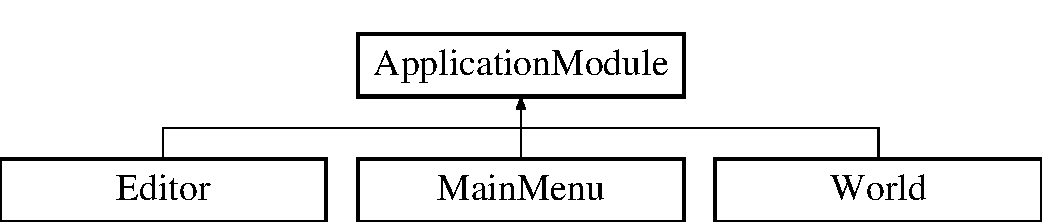
\includegraphics[height=2cm]{classApplicationModule}
\end{center}
\end{figure}
\subsection*{Public Member Functions}
\begin{DoxyCompactItemize}
\item 
\hyperlink{classApplicationModule_adee14a760314582348ee3205097fea4c}{ApplicationModule} (const CL\_\-DisplayWindow \&)
\item 
ApplicationModuleExitCode \hyperlink{classApplicationModule_a72494b92d2b093e0827893f527535a1f}{run} (void)
\item 
\hypertarget{classApplicationModule_a2c4555686e9bd25708a112ac852c3a17}{
CL\_\-GraphicContext $\ast$ {\bfseries get\_\-gc} (void)}
\label{classApplicationModule_a2c4555686e9bd25708a112ac852c3a17}

\item 
\hypertarget{classApplicationModule_a6c9168a94ebee4eacc23b7ce58878ce7}{
CL\_\-GUIManager $\ast$ {\bfseries get\_\-gui\_\-manager} (void)}
\label{classApplicationModule_a6c9168a94ebee4eacc23b7ce58878ce7}

\end{DoxyCompactItemize}
\subsection*{Protected Member Functions}
\begin{DoxyCompactItemize}
\item 
\hypertarget{classApplicationModule_a8976aad9f18518a03d83be61283d9b6e}{
virtual void {\bfseries draw} (void)}
\label{classApplicationModule_a8976aad9f18518a03d83be61283d9b6e}

\item 
\hypertarget{classApplicationModule_a1bfe895c2c5f3d14e32973db2ec51723}{
virtual void {\bfseries update} (void)}
\label{classApplicationModule_a1bfe895c2c5f3d14e32973db2ec51723}

\item 
\hypertarget{classApplicationModule_ac182827a21ffdafb13327e24c3aff773}{
virtual void {\bfseries wm\_\-repaint} (void)}
\label{classApplicationModule_ac182827a21ffdafb13327e24c3aff773}

\item 
void \hyperlink{classApplicationModule_a2fb74c01602d0a030eb7335543580be3}{draw\_\-loading} (void)
\item 
\hypertarget{classApplicationModule_ad21cf0501238dd52bbe4c84606f6cb91}{
virtual void {\bfseries on\_\-window\_\-close} (void)}
\label{classApplicationModule_ad21cf0501238dd52bbe4c84606f6cb91}

\item 
\hypertarget{classApplicationModule_aec7e75cf19261da574bc0f238b430738}{
virtual void {\bfseries on\_\-key\_\-down} (const CL\_\-InputEvent \&key, const CL\_\-InputState \&state)}
\label{classApplicationModule_aec7e75cf19261da574bc0f238b430738}

\item 
\hypertarget{classApplicationModule_acbff2a3dc36d72449a47ac0bb139719b}{
virtual void {\bfseries on\_\-key\_\-up} (const CL\_\-InputEvent \&key, const CL\_\-InputState \&state)}
\label{classApplicationModule_acbff2a3dc36d72449a47ac0bb139719b}

\item 
\hypertarget{classApplicationModule_a59c95ac03dc85010f132d5bbb628a481}{
virtual void {\bfseries on\_\-mouse\_\-down} (const CL\_\-InputEvent \&key, const CL\_\-InputState \&state)}
\label{classApplicationModule_a59c95ac03dc85010f132d5bbb628a481}

\item 
\hypertarget{classApplicationModule_a1017f6c73e46f9e2167ad71960bece8d}{
virtual void {\bfseries on\_\-mouse\_\-up} (const CL\_\-InputEvent \&key, const CL\_\-InputState \&state)}
\label{classApplicationModule_a1017f6c73e46f9e2167ad71960bece8d}

\item 
\hypertarget{classApplicationModule_a8da8b878817e13200ec732306ae412d9}{
virtual void {\bfseries on\_\-mouse\_\-move} (const CL\_\-InputEvent \&key, const CL\_\-InputState \&state)}
\label{classApplicationModule_a8da8b878817e13200ec732306ae412d9}

\item 
unsigned int \hyperlink{classApplicationModule_ab6e817b3b78e6563a446fae8e8abefb6}{get\_\-time\_\-elapsed} (void)
\end{DoxyCompactItemize}
\subsection*{Protected Attributes}
\begin{DoxyCompactItemize}
\item 
\hypertarget{classApplicationModule_a148d32ab67b53a89631ca60514dac4a6}{
ApplicationModuleExitCode {\bfseries exit\_\-code}}
\label{classApplicationModule_a148d32ab67b53a89631ca60514dac4a6}

\item 
\hypertarget{classApplicationModule_acf67b00ada6051624eab16d1594447e4}{
CL\_\-DisplayWindow {\bfseries window}}
\label{classApplicationModule_acf67b00ada6051624eab16d1594447e4}

\item 
\hypertarget{classApplicationModule_a507dc5dce4df518924b9a88f1816f6e5}{
CL\_\-GUIThemeDefault {\bfseries gui\_\-theme}}
\label{classApplicationModule_a507dc5dce4df518924b9a88f1816f6e5}

\item 
\hypertarget{classApplicationModule_a0169726ad6be80b99e933cdb629e73cf}{
CL\_\-ResourceManager {\bfseries gui\_\-rm}}
\label{classApplicationModule_a0169726ad6be80b99e933cdb629e73cf}

\item 
\hypertarget{classApplicationModule_a24ca28ca6ca0b1fc9ff54115c4d7f1aa}{
CL\_\-GUIWindowManagerTexture {\bfseries wm}}
\label{classApplicationModule_a24ca28ca6ca0b1fc9ff54115c4d7f1aa}

\item 
\hypertarget{classApplicationModule_a615058f2f96167dcfdefb98e711a7197}{
CL\_\-GUIManager {\bfseries gui}}
\label{classApplicationModule_a615058f2f96167dcfdefb98e711a7197}

\item 
\hypertarget{classApplicationModule_a847a964b766c02650275136054fbf2cf}{
CL\_\-GraphicContext {\bfseries gc}}
\label{classApplicationModule_a847a964b766c02650275136054fbf2cf}

\item 
\hypertarget{classApplicationModule_aeb1efd5a0360aa4b0b631f0ecd73782e}{
CL\_\-Slot {\bfseries slot\_\-quit}}
\label{classApplicationModule_aeb1efd5a0360aa4b0b631f0ecd73782e}

\item 
\hypertarget{classApplicationModule_ae1ec82a52e36716d11cf1ac25d4e81ac}{
CL\_\-Slot {\bfseries slot\_\-key\_\-down}}
\label{classApplicationModule_ae1ec82a52e36716d11cf1ac25d4e81ac}

\item 
\hypertarget{classApplicationModule_a7982a5f4dc5cc214a68646a545df3ea9}{
CL\_\-Slot {\bfseries slot\_\-key\_\-up}}
\label{classApplicationModule_a7982a5f4dc5cc214a68646a545df3ea9}

\item 
\hypertarget{classApplicationModule_aed41a09f76c702164b8f8ebdae86f830}{
CL\_\-Slot {\bfseries slot\_\-mouse\_\-down}}
\label{classApplicationModule_aed41a09f76c702164b8f8ebdae86f830}

\item 
\hypertarget{classApplicationModule_a716f59e33bd1c6b2ec0705428b7b280f}{
CL\_\-Slot {\bfseries slot\_\-mouse\_\-up}}
\label{classApplicationModule_a716f59e33bd1c6b2ec0705428b7b280f}

\item 
\hypertarget{classApplicationModule_abea0d9e41cec16a012776ceb78dd9348}{
CL\_\-Slot {\bfseries slot\_\-mouse\_\-move}}
\label{classApplicationModule_abea0d9e41cec16a012776ceb78dd9348}

\end{DoxyCompactItemize}


\subsection{Detailed Description}
An \hyperlink{classApplicationModule}{ApplicationModule} represents part of the overall application where all inherent classes would not expect to be instantiated at the same time but share common components, such as a window manager, gui object, graphics context, input slots, a \char`\"{}run\char`\"{} function to initiate the loop and a class variable for breaking the loop.

This ensures that the editor and the game do not have to repeat this common code and instead inherit this object. 

\subsection{Constructor \& Destructor Documentation}
\hypertarget{classApplicationModule_adee14a760314582348ee3205097fea4c}{
\index{ApplicationModule@{ApplicationModule}!ApplicationModule@{ApplicationModule}}
\index{ApplicationModule@{ApplicationModule}!ApplicationModule@{ApplicationModule}}
\subsubsection[{ApplicationModule}]{\setlength{\rightskip}{0pt plus 5cm}ApplicationModule::ApplicationModule (const CL\_\-DisplayWindow \& {\em display\_\-window})}}
\label{classApplicationModule_adee14a760314582348ee3205097fea4c}
Prepares object and displays loading message. 

\subsection{Member Function Documentation}
\hypertarget{classApplicationModule_a2fb74c01602d0a030eb7335543580be3}{
\index{ApplicationModule@{ApplicationModule}!draw\_\-loading@{draw\_\-loading}}
\index{draw\_\-loading@{draw\_\-loading}!ApplicationModule@{ApplicationModule}}
\subsubsection[{draw\_\-loading}]{\setlength{\rightskip}{0pt plus 5cm}void ApplicationModule::draw\_\-loading (void)\hspace{0.3cm}{\ttfamily  \mbox{[}protected\mbox{]}}}}
\label{classApplicationModule_a2fb74c01602d0a030eb7335543580be3}
Draws the loading screen on the graphics context. \hypertarget{classApplicationModule_ab6e817b3b78e6563a446fae8e8abefb6}{
\index{ApplicationModule@{ApplicationModule}!get\_\-time\_\-elapsed@{get\_\-time\_\-elapsed}}
\index{get\_\-time\_\-elapsed@{get\_\-time\_\-elapsed}!ApplicationModule@{ApplicationModule}}
\subsubsection[{get\_\-time\_\-elapsed}]{\setlength{\rightskip}{0pt plus 5cm}unsigned int ApplicationModule::get\_\-time\_\-elapsed (void)\hspace{0.3cm}{\ttfamily  \mbox{[}protected\mbox{]}}}}
\label{classApplicationModule_ab6e817b3b78e6563a446fae8e8abefb6}
Calculate amount of time since the last call. \hypertarget{classApplicationModule_a72494b92d2b093e0827893f527535a1f}{
\index{ApplicationModule@{ApplicationModule}!run@{run}}
\index{run@{run}!ApplicationModule@{ApplicationModule}}
\subsubsection[{run}]{\setlength{\rightskip}{0pt plus 5cm}ApplicationModuleExitCode ApplicationModule::run (void)}}
\label{classApplicationModule_a72494b92d2b093e0827893f527535a1f}
Initiates the main loop. Does not render the GUI it is down the the inherent classes to do so. 

The documentation for this class was generated from the following files:\begin{DoxyCompactItemize}
\item 
source/\hyperlink{ApplicationModule_8h}{ApplicationModule.h}\item 
source/\hyperlink{ApplicationModule_8cpp}{ApplicationModule.cpp}\end{DoxyCompactItemize}

\hypertarget{classdlib_1_1array}{
\section{dlib::array$<$ T, mem\_\-manager $>$ Class Template Reference}
\label{classdlib_1_1array}\index{dlib::array@{dlib::array}}
}
\subsection*{Public Types}
\begin{DoxyCompactItemize}
\item 
\hypertarget{classdlib_1_1array_adc0c8cb12a28d10432a13d9eb4c6a487}{
typedef array\_\-kernel\_\-1$<$ T, mem\_\-manager $>$ {\bfseries kernel\_\-1a}}
\label{classdlib_1_1array_adc0c8cb12a28d10432a13d9eb4c6a487}

\item 
\hypertarget{classdlib_1_1array_a5d1b2ce2c97c5ce3457e187ff5c36faa}{
typedef array\_\-kernel\_\-c$<$ kernel\_\-1a $>$ {\bfseries kernel\_\-1a\_\-c}}
\label{classdlib_1_1array_a5d1b2ce2c97c5ce3457e187ff5c36faa}

\item 
\hypertarget{classdlib_1_1array_a5bb3005a519346d4c6b832e4b52755e4}{
typedef array\_\-kernel\_\-2$<$ T, mem\_\-manager $>$ {\bfseries kernel\_\-2a}}
\label{classdlib_1_1array_a5bb3005a519346d4c6b832e4b52755e4}

\item 
\hypertarget{classdlib_1_1array_a40729228e2f077371be2d31e61da5668}{
typedef array\_\-kernel\_\-c$<$ kernel\_\-2a $>$ {\bfseries kernel\_\-2a\_\-c}}
\label{classdlib_1_1array_a40729228e2f077371be2d31e61da5668}

\item 
\hypertarget{classdlib_1_1array_a7a44fa9401279068de3cb18e530ad85a}{
typedef array\_\-sort\_\-1$<$ kernel\_\-1a $>$ {\bfseries sort\_\-1a}}
\label{classdlib_1_1array_a7a44fa9401279068de3cb18e530ad85a}

\item 
\hypertarget{classdlib_1_1array_a834ad38a72079497a6943283a9ce1d19}{
typedef array\_\-sort\_\-1$<$ kernel\_\-1a\_\-c $>$ {\bfseries sort\_\-1a\_\-c}}
\label{classdlib_1_1array_a834ad38a72079497a6943283a9ce1d19}

\item 
\hypertarget{classdlib_1_1array_a86a19518b536ef6e479f671cdf51c098}{
typedef array\_\-sort\_\-1$<$ kernel\_\-2a $>$ {\bfseries sort\_\-1b}}
\label{classdlib_1_1array_a86a19518b536ef6e479f671cdf51c098}

\item 
\hypertarget{classdlib_1_1array_aab01d3f68430e4eb706cf1120111c4ad}{
typedef array\_\-sort\_\-1$<$ kernel\_\-2a\_\-c $>$ {\bfseries sort\_\-1b\_\-c}}
\label{classdlib_1_1array_aab01d3f68430e4eb706cf1120111c4ad}

\item 
\hypertarget{classdlib_1_1array_a9b73b3e6c395f37de471a1c126fdfc5c}{
typedef array\_\-sort\_\-2$<$ kernel\_\-1a $>$ {\bfseries sort\_\-2a}}
\label{classdlib_1_1array_a9b73b3e6c395f37de471a1c126fdfc5c}

\item 
\hypertarget{classdlib_1_1array_ac5f19e38041d0ce69ede54f602d06e1b}{
typedef array\_\-sort\_\-2$<$ kernel\_\-1a\_\-c $>$ {\bfseries sort\_\-2a\_\-c}}
\label{classdlib_1_1array_ac5f19e38041d0ce69ede54f602d06e1b}

\item 
\hypertarget{classdlib_1_1array_a47bbbbe6627a7b091315bd887352f1a3}{
typedef array\_\-sort\_\-2$<$ kernel\_\-2a $>$ {\bfseries sort\_\-2b}}
\label{classdlib_1_1array_a47bbbbe6627a7b091315bd887352f1a3}

\item 
\hypertarget{classdlib_1_1array_a82877adabfb3dab98a6092b3c5b384f2}{
typedef array\_\-sort\_\-2$<$ kernel\_\-2a\_\-c $>$ {\bfseries sort\_\-2b\_\-c}}
\label{classdlib_1_1array_a82877adabfb3dab98a6092b3c5b384f2}

\item 
\hypertarget{classdlib_1_1array_a8bef642089b1615c619d7dbb841b489e}{
typedef array\_\-expand\_\-1$<$ sort\_\-1a $>$ {\bfseries expand\_\-1a}}
\label{classdlib_1_1array_a8bef642089b1615c619d7dbb841b489e}

\item 
\hypertarget{classdlib_1_1array_a3c8253f1535d9e849f7130eb81acbc28}{
typedef array\_\-expand\_\-c$<$ array\_\-kernel\_\-c$<$ expand\_\-1a $>$ $>$ {\bfseries expand\_\-1a\_\-c}}
\label{classdlib_1_1array_a3c8253f1535d9e849f7130eb81acbc28}

\item 
\hypertarget{classdlib_1_1array_a74db12d11aab1af94dfcbff8b9d4cbe5}{
typedef array\_\-expand\_\-1$<$ sort\_\-1b $>$ {\bfseries expand\_\-1b}}
\label{classdlib_1_1array_a74db12d11aab1af94dfcbff8b9d4cbe5}

\item 
\hypertarget{classdlib_1_1array_af116da0897cd6dfd8cc5216fa9ffdb19}{
typedef array\_\-expand\_\-c$<$ array\_\-kernel\_\-c$<$ expand\_\-1b $>$ $>$ {\bfseries expand\_\-1b\_\-c}}
\label{classdlib_1_1array_af116da0897cd6dfd8cc5216fa9ffdb19}

\item 
\hypertarget{classdlib_1_1array_a6bca4760c81d9ab9bae6d0cfb2b982e6}{
typedef array\_\-expand\_\-1$<$ sort\_\-2a $>$ {\bfseries expand\_\-1c}}
\label{classdlib_1_1array_a6bca4760c81d9ab9bae6d0cfb2b982e6}

\item 
\hypertarget{classdlib_1_1array_a9b0cd9262892e1af7da5f3729d3bd10e}{
typedef array\_\-expand\_\-c$<$ array\_\-kernel\_\-c$<$ expand\_\-1c $>$ $>$ {\bfseries expand\_\-1c\_\-c}}
\label{classdlib_1_1array_a9b0cd9262892e1af7da5f3729d3bd10e}

\item 
\hypertarget{classdlib_1_1array_a3861701cab061706f223102d86d15f49}{
typedef array\_\-expand\_\-1$<$ sort\_\-2b $>$ {\bfseries expand\_\-1d}}
\label{classdlib_1_1array_a3861701cab061706f223102d86d15f49}

\item 
\hypertarget{classdlib_1_1array_a9ab175ddbb854eed876e3a45d903fca9}{
typedef array\_\-expand\_\-c$<$ array\_\-kernel\_\-c$<$ expand\_\-1d $>$ $>$ {\bfseries expand\_\-1d\_\-c}}
\label{classdlib_1_1array_a9ab175ddbb854eed876e3a45d903fca9}

\end{DoxyCompactItemize}
\subsubsection*{template$<$typename T, typename mem\_\-manager = memory\_\-manager$<$char$>$::kernel\_\-1a$>$ class dlib::array$<$ T, mem\_\-manager $>$}



The documentation for this class was generated from the following file:\begin{DoxyCompactItemize}
\item 
source/dlib/array.h\end{DoxyCompactItemize}

\hypertarget{classdlib_1_1array2d}{
\section{dlib::array2d$<$ T, mem\_\-manager $>$ Class Template Reference}
\label{classdlib_1_1array2d}\index{dlib::array2d@{dlib::array2d}}
}
\subsection*{Public Types}
\begin{DoxyCompactItemize}
\item 
\hypertarget{classdlib_1_1array2d_a2c111db63374b88dae1b67cbe13af120}{
typedef array2d\_\-kernel\_\-1$<$ T, mem\_\-manager $>$ {\bfseries kernel\_\-1a}}
\label{classdlib_1_1array2d_a2c111db63374b88dae1b67cbe13af120}

\item 
\hypertarget{classdlib_1_1array2d_a002e42285ca5401721ec363c2b723217}{
typedef array2d\_\-kernel\_\-c$<$ kernel\_\-1a $>$ {\bfseries kernel\_\-1a\_\-c}}
\label{classdlib_1_1array2d_a002e42285ca5401721ec363c2b723217}

\end{DoxyCompactItemize}
\subsubsection*{template$<$typename T, typename mem\_\-manager = memory\_\-manager$<$char$>$::kernel\_\-1a$>$ class dlib::array2d$<$ T, mem\_\-manager $>$}



The documentation for this class was generated from the following file:\begin{DoxyCompactItemize}
\item 
source/dlib/array2d.h\end{DoxyCompactItemize}

\hypertarget{structdlib_1_1assert__are__not__same__type}{
\section{dlib::assert\_\-are\_\-not\_\-same\_\-type$<$ T, U $>$ Struct Template Reference}
\label{structdlib_1_1assert__are__not__same__type}\index{dlib::assert\_\-are\_\-not\_\-same\_\-type@{dlib::assert\_\-are\_\-not\_\-same\_\-type}}
}
\subsection*{Public Types}
\begin{DoxyCompactItemize}
\item 
enum \{ {\bfseries value} = 1
 \}
\end{DoxyCompactItemize}
\subsubsection*{template$<$typename T, typename U$>$ struct dlib::assert\_\-are\_\-not\_\-same\_\-type$<$ T, U $>$}



The documentation for this struct was generated from the following file:\begin{DoxyCompactItemize}
\item 
source/dlib/assert.h\end{DoxyCompactItemize}

\hypertarget{structdlib_1_1assert__are__not__same__type_3_01T_00_01T_01_4}{
\section{dlib::assert\_\-are\_\-not\_\-same\_\-type$<$ T, T $>$ Struct Template Reference}
\label{structdlib_1_1assert__are__not__same__type_3_01T_00_01T_01_4}\index{dlib::assert\_\-are\_\-not\_\-same\_\-type$<$ T, T $>$@{dlib::assert\_\-are\_\-not\_\-same\_\-type$<$ T, T $>$}}
}
\subsubsection*{template$<$typename T$>$ struct dlib::assert\_\-are\_\-not\_\-same\_\-type$<$ T, T $>$}



The documentation for this struct was generated from the following file:\begin{DoxyCompactItemize}
\item 
source/dlib/assert.h\end{DoxyCompactItemize}

\hypertarget{structdlib_1_1assert__are__same__type_3_01T_00_01T_01_4}{
\section{dlib::assert\_\-are\_\-same\_\-type$<$ T, T $>$ Struct Template Reference}
\label{structdlib_1_1assert__are__same__type_3_01T_00_01T_01_4}\index{dlib::assert\_\-are\_\-same\_\-type$<$ T, T $>$@{dlib::assert\_\-are\_\-same\_\-type$<$ T, T $>$}}
}
\subsection*{Public Types}
\begin{DoxyCompactItemize}
\item 
enum \{ {\bfseries value} = 1
 \}
\end{DoxyCompactItemize}
\subsubsection*{template$<$typename T$>$ struct dlib::assert\_\-are\_\-same\_\-type$<$ T, T $>$}



The documentation for this struct was generated from the following file:\begin{DoxyCompactItemize}
\item 
source/dlib/assert.h\end{DoxyCompactItemize}

\hypertarget{classdlib_1_1assignment}{
\section{dlib::assignment Class Reference}
\label{classdlib_1_1assignment}\index{dlib::assignment@{dlib::assignment}}
}
\subsection*{Public Member Functions}
\begin{DoxyCompactItemize}
\item 
\hypertarget{classdlib_1_1assignment_a71173dd08edc8bb2a063b207cba1d3f4}{
{\bfseries assignment} (const \hyperlink{classdlib_1_1assignment}{assignment} \&a)}
\label{classdlib_1_1assignment_a71173dd08edc8bb2a063b207cba1d3f4}

\item 
\hypertarget{classdlib_1_1assignment_aa9fc8e7b66424499b40d46263a9c7588}{
\hyperlink{classdlib_1_1assignment}{assignment} \& {\bfseries operator=} (const \hyperlink{classdlib_1_1assignment}{assignment} \&rhs)}
\label{classdlib_1_1assignment_aa9fc8e7b66424499b40d46263a9c7588}

\item 
\hypertarget{classdlib_1_1assignment_ab045b6e4070f1eac80c8c5291643ba28}{
void {\bfseries clear} ()}
\label{classdlib_1_1assignment_ab045b6e4070f1eac80c8c5291643ba28}

\item 
\hypertarget{classdlib_1_1assignment_a6a728f803e5a94351a6b91d039d532de}{
bool {\bfseries operator$<$} (const \hyperlink{classdlib_1_1assignment}{assignment} \&item) const }
\label{classdlib_1_1assignment_a6a728f803e5a94351a6b91d039d532de}

\item 
\hypertarget{classdlib_1_1assignment_a7029eba2c663f2ceacb66e2800db2a19}{
bool {\bfseries has\_\-index} (unsigned long idx) const }
\label{classdlib_1_1assignment_a7029eba2c663f2ceacb66e2800db2a19}

\item 
\hypertarget{classdlib_1_1assignment_abdf328b4deae98e8e8d91895805d534f}{
void {\bfseries add} (unsigned long idx, unsigned long value=0)}
\label{classdlib_1_1assignment_abdf328b4deae98e8e8d91895805d534f}

\item 
\hypertarget{classdlib_1_1assignment_a2dc646524f0dc2ff2db657e3de716f72}{
unsigned long \& {\bfseries operator\mbox{[}$\,$\mbox{]}} (const long idx)}
\label{classdlib_1_1assignment_a2dc646524f0dc2ff2db657e3de716f72}

\item 
\hypertarget{classdlib_1_1assignment_a18bf75e6c9ee1e9331ed060681ec364d}{
const unsigned long \& {\bfseries operator\mbox{[}$\,$\mbox{]}} (const long idx) const }
\label{classdlib_1_1assignment_a18bf75e6c9ee1e9331ed060681ec364d}

\item 
\hypertarget{classdlib_1_1assignment_ac4e11a39021bdaa13dba1fcfbee773a6}{
void {\bfseries swap} (\hyperlink{classdlib_1_1assignment}{assignment} \&item)}
\label{classdlib_1_1assignment_ac4e11a39021bdaa13dba1fcfbee773a6}

\item 
\hypertarget{classdlib_1_1assignment_a07d5568b7d6f4fdb0aa4ab286179b806}{
void {\bfseries remove} (unsigned long idx)}
\label{classdlib_1_1assignment_a07d5568b7d6f4fdb0aa4ab286179b806}

\item 
\hypertarget{classdlib_1_1assignment_adb14891314fee1f1723929fdec3efb01}{
unsigned long {\bfseries size} () const }
\label{classdlib_1_1assignment_adb14891314fee1f1723929fdec3efb01}

\item 
\hypertarget{classdlib_1_1assignment_aeecaf59a6ad760dd7bf640966fe1230b}{
void {\bfseries reset} () const }
\label{classdlib_1_1assignment_aeecaf59a6ad760dd7bf640966fe1230b}

\item 
\hypertarget{classdlib_1_1assignment_ab959307ab986673d4ab983e19a9c818c}{
bool {\bfseries move\_\-next} () const }
\label{classdlib_1_1assignment_ab959307ab986673d4ab983e19a9c818c}

\item 
\hypertarget{classdlib_1_1assignment_a2038496c149f5586140466b06cf49c5b}{
map\_\-pair$<$ unsigned long, unsigned long $>$ \& {\bfseries element} ()}
\label{classdlib_1_1assignment_a2038496c149f5586140466b06cf49c5b}

\item 
\hypertarget{classdlib_1_1assignment_a83af025bdb1c87104924c25a11c51ff7}{
const map\_\-pair$<$ unsigned long, unsigned long $>$ \& {\bfseries element} () const }
\label{classdlib_1_1assignment_a83af025bdb1c87104924c25a11c51ff7}

\item 
\hypertarget{classdlib_1_1assignment_afea92a3eadc591c0f94188d1a9b29454}{
bool {\bfseries at\_\-start} () const }
\label{classdlib_1_1assignment_afea92a3eadc591c0f94188d1a9b29454}

\item 
\hypertarget{classdlib_1_1assignment_a20d81215cd5da8b44268084fc2724fe9}{
bool {\bfseries current\_\-element\_\-valid} () const }
\label{classdlib_1_1assignment_a20d81215cd5da8b44268084fc2724fe9}

\end{DoxyCompactItemize}
\subsection*{Friends}
\begin{DoxyCompactItemize}
\item 
\hypertarget{classdlib_1_1assignment_ad9af354e7caed6401c9fad702aff05e1}{
void {\bfseries serialize} (const \hyperlink{classdlib_1_1assignment}{assignment} \&item, std::ostream \&out)}
\label{classdlib_1_1assignment_ad9af354e7caed6401c9fad702aff05e1}

\item 
\hypertarget{classdlib_1_1assignment_a7d9bcb8be8dbcdbfa3b14d8f434aacad}{
void {\bfseries deserialize} (\hyperlink{classdlib_1_1assignment}{assignment} \&item, std::istream \&in)}
\label{classdlib_1_1assignment_a7d9bcb8be8dbcdbfa3b14d8f434aacad}

\end{DoxyCompactItemize}


The documentation for this class was generated from the following file:\begin{DoxyCompactItemize}
\item 
source/dlib/bayes\_\-utils/bayes\_\-utils.h\end{DoxyCompactItemize}

\hypertarget{classdlib_1_1base64}{
\section{dlib::base64 Class Reference}
\label{classdlib_1_1base64}\index{dlib::base64@{dlib::base64}}
}
\subsection*{Public Types}
\begin{DoxyCompactItemize}
\item 
\hypertarget{classdlib_1_1base64_a393d53526eb0f7b4189b93b8eab9f8ed}{
typedef base64\_\-kernel\_\-1 {\bfseries kernel\_\-1a}}
\label{classdlib_1_1base64_a393d53526eb0f7b4189b93b8eab9f8ed}

\end{DoxyCompactItemize}


The documentation for this class was generated from the following file:\begin{DoxyCompactItemize}
\item 
source/dlib/base64.h\end{DoxyCompactItemize}

\hypertarget{classdlib_1_1bayes__node}{
\section{dlib::bayes\_\-node Class Reference}
\label{classdlib_1_1bayes__node}\index{dlib::bayes\_\-node@{dlib::bayes\_\-node}}
}


Inherits boost::noncopyable.\subsection*{Public Member Functions}
\begin{DoxyCompactItemize}
\item 
\hypertarget{classdlib_1_1bayes__node_af0f4424ec96f869df6afee921f880796}{
unsigned long {\bfseries value} () const }
\label{classdlib_1_1bayes__node_af0f4424ec96f869df6afee921f880796}

\item 
\hypertarget{classdlib_1_1bayes__node_ad128a535311efa22a443c5df64de226b}{
void {\bfseries set\_\-value} (unsigned long new\_\-value)}
\label{classdlib_1_1bayes__node_ad128a535311efa22a443c5df64de226b}

\item 
\hypertarget{classdlib_1_1bayes__node_a402ff3dd0031445fedc29a0eb78369ea}{
\hyperlink{classdlib_1_1conditional__probability__table}{conditional\_\-probability\_\-table} \& {\bfseries table} ()}
\label{classdlib_1_1bayes__node_a402ff3dd0031445fedc29a0eb78369ea}

\item 
\hypertarget{classdlib_1_1bayes__node_a542c00603222cc1d12a9014b3276b7b6}{
const \hyperlink{classdlib_1_1conditional__probability__table}{conditional\_\-probability\_\-table} \& {\bfseries table} () const }
\label{classdlib_1_1bayes__node_a542c00603222cc1d12a9014b3276b7b6}

\item 
\hypertarget{classdlib_1_1bayes__node_a614113e5fbf2e71f28fcce3d2593bd13}{
bool {\bfseries is\_\-evidence} () const }
\label{classdlib_1_1bayes__node_a614113e5fbf2e71f28fcce3d2593bd13}

\item 
\hypertarget{classdlib_1_1bayes__node_a9fb1f50ecc46d11d7ea60aa69513d204}{
void {\bfseries set\_\-as\_\-nonevidence} ()}
\label{classdlib_1_1bayes__node_a9fb1f50ecc46d11d7ea60aa69513d204}

\item 
\hypertarget{classdlib_1_1bayes__node_a13d6fd593abe483fb70fc2702d6287e1}{
void {\bfseries set\_\-as\_\-evidence} ()}
\label{classdlib_1_1bayes__node_a13d6fd593abe483fb70fc2702d6287e1}

\item 
\hypertarget{classdlib_1_1bayes__node_ae6991652466762454c7ea8ac0abfddd6}{
void {\bfseries swap} (\hyperlink{classdlib_1_1bayes__node}{bayes\_\-node} \&item)}
\label{classdlib_1_1bayes__node_ae6991652466762454c7ea8ac0abfddd6}

\end{DoxyCompactItemize}
\subsection*{Friends}
\begin{DoxyCompactItemize}
\item 
\hypertarget{classdlib_1_1bayes__node_afa25c2d742bf3c9d80deb7d965755a39}{
void {\bfseries serialize} (const \hyperlink{classdlib_1_1bayes__node}{bayes\_\-node} \&item, std::ostream \&out)}
\label{classdlib_1_1bayes__node_afa25c2d742bf3c9d80deb7d965755a39}

\item 
\hypertarget{classdlib_1_1bayes__node_a18a0d688066c0e223ad844ee44ff2cbb}{
void {\bfseries deserialize} (\hyperlink{classdlib_1_1bayes__node}{bayes\_\-node} \&item, std::istream \&in)}
\label{classdlib_1_1bayes__node_a18a0d688066c0e223ad844ee44ff2cbb}

\end{DoxyCompactItemize}


The documentation for this class was generated from the following file:\begin{DoxyCompactItemize}
\item 
source/dlib/bayes\_\-utils/bayes\_\-utils.h\end{DoxyCompactItemize}

\hypertarget{classdlib_1_1bayesian__network__gibbs__sampler}{
\section{dlib::bayesian\_\-network\_\-gibbs\_\-sampler Class Reference}
\label{classdlib_1_1bayesian__network__gibbs__sampler}\index{dlib::bayesian\_\-network\_\-gibbs\_\-sampler@{dlib::bayesian\_\-network\_\-gibbs\_\-sampler}}
}


Inherits boost::noncopyable.\subsection*{Public Member Functions}
\begin{DoxyCompactItemize}
\item 
\hypertarget{classdlib_1_1bayesian__network__gibbs__sampler_a6623356f6ceed89ee20455ea27cd723f}{
{\footnotesize template$<$typename T $>$ }\\void {\bfseries sample\_\-graph} (T \&bn)}
\label{classdlib_1_1bayesian__network__gibbs__sampler_a6623356f6ceed89ee20455ea27cd723f}

\end{DoxyCompactItemize}


The documentation for this class was generated from the following file:\begin{DoxyCompactItemize}
\item 
source/dlib/bayes\_\-utils/bayes\_\-utils.h\end{DoxyCompactItemize}

\hypertarget{classdlib_1_1bayesian__network__join__tree}{
\section{dlib::bayesian\_\-network\_\-join\_\-tree Class Reference}
\label{classdlib_1_1bayesian__network__join__tree}\index{dlib::bayesian\_\-network\_\-join\_\-tree@{dlib::bayesian\_\-network\_\-join\_\-tree}}
}


Inherits boost::noncopyable.\subsection*{Public Member Functions}
\begin{DoxyCompactItemize}
\item 
{\footnotesize template$<$typename T , typename U $>$ }\\\hyperlink{classdlib_1_1bayesian__network__join__tree_a7667669c480712d31dcb0ee332491a63}{bayesian\_\-network\_\-join\_\-tree} (const T \&bn, const U \&join\_\-tree)
\item 
\hypertarget{classdlib_1_1bayesian__network__join__tree_a1cf444cf6be8e4288508ee0e815b78d1}{
const matrix$<$ double, 1 $>$ {\bfseries probability} (unsigned long idx) const }
\label{classdlib_1_1bayesian__network__join__tree_a1cf444cf6be8e4288508ee0e815b78d1}

\item 
\hypertarget{classdlib_1_1bayesian__network__join__tree_a744e39b94161de2d16501f40a9361e99}{
unsigned long {\bfseries number\_\-of\_\-nodes} () const }
\label{classdlib_1_1bayesian__network__join__tree_a744e39b94161de2d16501f40a9361e99}

\item 
\hypertarget{classdlib_1_1bayesian__network__join__tree_a2eb88fb81971daa218a300056d5ac305}{
void {\bfseries swap} (\hyperlink{classdlib_1_1bayesian__network__join__tree}{bayesian\_\-network\_\-join\_\-tree} \&item)}
\label{classdlib_1_1bayesian__network__join__tree_a2eb88fb81971daa218a300056d5ac305}

\end{DoxyCompactItemize}


\subsection{Constructor \& Destructor Documentation}
\hypertarget{classdlib_1_1bayesian__network__join__tree_a7667669c480712d31dcb0ee332491a63}{
\index{dlib::bayesian\_\-network\_\-join\_\-tree@{dlib::bayesian\_\-network\_\-join\_\-tree}!bayesian\_\-network\_\-join\_\-tree@{bayesian\_\-network\_\-join\_\-tree}}
\index{bayesian\_\-network\_\-join\_\-tree@{bayesian\_\-network\_\-join\_\-tree}!dlib::bayesian_network_join_tree@{dlib::bayesian\_\-network\_\-join\_\-tree}}
\subsubsection[{bayesian\_\-network\_\-join\_\-tree}]{\setlength{\rightskip}{0pt plus 5cm}template$<$typename T , typename U $>$ dlib::bayesian\_\-network\_\-join\_\-tree::bayesian\_\-network\_\-join\_\-tree (const T \& {\em bn}, \/  const U \& {\em join\_\-tree})\hspace{0.3cm}{\ttfamily  \mbox{[}inline\mbox{]}}}}
\label{classdlib_1_1bayesian__network__join__tree_a7667669c480712d31dcb0ee332491a63}
use the pimpl idiom to push the template arguments from the class level to the constructor level ! 

The documentation for this class was generated from the following file:\begin{DoxyCompactItemize}
\item 
source/dlib/bayes\_\-utils/bayes\_\-utils.h\end{DoxyCompactItemize}

\hypertarget{structdlib_1_1bgr__pixel}{
\section{dlib::bgr\_\-pixel Struct Reference}
\label{structdlib_1_1bgr__pixel}\index{dlib::bgr\_\-pixel@{dlib::bgr\_\-pixel}}
}
\subsection*{Public Member Functions}
\begin{DoxyCompactItemize}
\item 
\hyperlink{structdlib_1_1bgr__pixel_a525b55be99d6be3a3a14d7b111f68708}{bgr\_\-pixel} ()
\item 
\hypertarget{structdlib_1_1bgr__pixel_a58a50096a7d29c76064b690f8709a621}{
{\bfseries bgr\_\-pixel} (unsigned char blue\_\-, unsigned char green\_\-, unsigned char red\_\-)}
\label{structdlib_1_1bgr__pixel_a58a50096a7d29c76064b690f8709a621}

\end{DoxyCompactItemize}
\subsection*{Public Attributes}
\begin{DoxyCompactItemize}
\item 
\hypertarget{structdlib_1_1bgr__pixel_ac6015d194beed3146cbc0db6fb50ea70}{
unsigned char {\bfseries blue}}
\label{structdlib_1_1bgr__pixel_ac6015d194beed3146cbc0db6fb50ea70}

\item 
\hypertarget{structdlib_1_1bgr__pixel_aa71b50bb0288cfcf07fc26c9d83c0efa}{
unsigned char {\bfseries green}}
\label{structdlib_1_1bgr__pixel_aa71b50bb0288cfcf07fc26c9d83c0efa}

\item 
\hypertarget{structdlib_1_1bgr__pixel_a3f7b74e4be61cbd0cf3b7d8809f4245a}{
unsigned char {\bfseries red}}
\label{structdlib_1_1bgr__pixel_a3f7b74e4be61cbd0cf3b7d8809f4245a}

\end{DoxyCompactItemize}


\subsection{Constructor \& Destructor Documentation}
\hypertarget{structdlib_1_1bgr__pixel_a525b55be99d6be3a3a14d7b111f68708}{
\index{dlib::bgr\_\-pixel@{dlib::bgr\_\-pixel}!bgr\_\-pixel@{bgr\_\-pixel}}
\index{bgr\_\-pixel@{bgr\_\-pixel}!dlib::bgr_pixel@{dlib::bgr\_\-pixel}}
\subsubsection[{bgr\_\-pixel}]{\setlength{\rightskip}{0pt plus 5cm}dlib::bgr\_\-pixel::bgr\_\-pixel ()\hspace{0.3cm}{\ttfamily  \mbox{[}inline\mbox{]}}}}
\label{structdlib_1_1bgr__pixel_a525b55be99d6be3a3a14d7b111f68708}
WHAT THIS OBJECT REPRESENTS This is a simple struct that represents an BGR colored graphical pixel. (the reason it exists in addition to the \hyperlink{structdlib_1_1rgb__pixel}{rgb\_\-pixel} is so you can lay it down on top of a memory region that organizes its color data in the BGR format and still be able to read it) ! 

The documentation for this struct was generated from the following file:\begin{DoxyCompactItemize}
\item 
source/dlib/pixel.h\end{DoxyCompactItemize}

\hypertarget{classdlib_1_1bigint}{
\section{dlib::bigint Class Reference}
\label{classdlib_1_1bigint}\index{dlib::bigint@{dlib::bigint}}
}
\subsection*{Public Types}
\begin{DoxyCompactItemize}
\item 
\hypertarget{classdlib_1_1bigint_ab2510bc3838b7287df5c41af8e51b1b1}{
typedef bigint\_\-kernel\_\-1 {\bfseries kernel\_\-1a}}
\label{classdlib_1_1bigint_ab2510bc3838b7287df5c41af8e51b1b1}

\item 
\hypertarget{classdlib_1_1bigint_a28e0e3d8acfc1dd2b39dffa27ba7d6cf}{
typedef bigint\_\-kernel\_\-c$<$ kernel\_\-1a $>$ {\bfseries kernel\_\-1a\_\-c}}
\label{classdlib_1_1bigint_a28e0e3d8acfc1dd2b39dffa27ba7d6cf}

\item 
\hypertarget{classdlib_1_1bigint_a3c66aa0ba3b40a128e75747636547257}{
typedef bigint\_\-kernel\_\-2 {\bfseries kernel\_\-2a}}
\label{classdlib_1_1bigint_a3c66aa0ba3b40a128e75747636547257}

\item 
\hypertarget{classdlib_1_1bigint_a559c8024eab63ce144c0ec4ef5eb000f}{
typedef bigint\_\-kernel\_\-c$<$ kernel\_\-2a $>$ {\bfseries kernel\_\-2a\_\-c}}
\label{classdlib_1_1bigint_a559c8024eab63ce144c0ec4ef5eb000f}

\end{DoxyCompactItemize}


The documentation for this class was generated from the following file:\begin{DoxyCompactItemize}
\item 
source/dlib/bigint.h\end{DoxyCompactItemize}

\hypertarget{classdlib_1_1binary__search__tree}{
\section{dlib::binary\_\-search\_\-tree$<$ domain, range, mem\_\-manager, compare $>$ Class Template Reference}
\label{classdlib_1_1binary__search__tree}\index{dlib::binary\_\-search\_\-tree@{dlib::binary\_\-search\_\-tree}}
}
\subsection*{Public Types}
\begin{DoxyCompactItemize}
\item 
\hypertarget{classdlib_1_1binary__search__tree_a8948f5148f1352f2615025fe1e4e3c16}{
typedef binary\_\-search\_\-tree\_\-kernel\_\-1$<$ domain, range, mem\_\-manager, compare $>$ {\bfseries kernel\_\-1a}}
\label{classdlib_1_1binary__search__tree_a8948f5148f1352f2615025fe1e4e3c16}

\item 
\hypertarget{classdlib_1_1binary__search__tree_aa375ea38939f84497b3e94b9256b2909}{
typedef binary\_\-search\_\-tree\_\-kernel\_\-c$<$ kernel\_\-1a $>$ {\bfseries kernel\_\-1a\_\-c}}
\label{classdlib_1_1binary__search__tree_aa375ea38939f84497b3e94b9256b2909}

\item 
\hypertarget{classdlib_1_1binary__search__tree_abcc3cda8db16b8d85d89fa194f775831}{
typedef binary\_\-search\_\-tree\_\-kernel\_\-2$<$ domain, range, mem\_\-manager, compare $>$ {\bfseries kernel\_\-2a}}
\label{classdlib_1_1binary__search__tree_abcc3cda8db16b8d85d89fa194f775831}

\item 
\hypertarget{classdlib_1_1binary__search__tree_a26a8ebb2b6bf26ccdf7b70757db44f92}{
typedef binary\_\-search\_\-tree\_\-kernel\_\-c$<$ kernel\_\-2a $>$ {\bfseries kernel\_\-2a\_\-c}}
\label{classdlib_1_1binary__search__tree_a26a8ebb2b6bf26ccdf7b70757db44f92}

\end{DoxyCompactItemize}
\subsubsection*{template$<$typename domain, typename range, typename mem\_\-manager = memory\_\-manager$<$char$>$::kernel\_\-1a, typename compare = std::less$<$domain$>$$>$ class dlib::binary\_\-search\_\-tree$<$ domain, range, mem\_\-manager, compare $>$}



The documentation for this class was generated from the following file:\begin{DoxyCompactItemize}
\item 
source/dlib/binary\_\-search\_\-tree.h\end{DoxyCompactItemize}

\hypertarget{classdlib_1_1bit__stream}{
\section{dlib::bit\_\-stream Class Reference}
\label{classdlib_1_1bit__stream}\index{dlib::bit\_\-stream@{dlib::bit\_\-stream}}
}
\subsection*{Public Types}
\begin{DoxyCompactItemize}
\item 
\hypertarget{classdlib_1_1bit__stream_a6bc419948ff65bfeaf389191b69d725a}{
typedef bit\_\-stream\_\-kernel\_\-1 {\bfseries kernel\_\-1a}}
\label{classdlib_1_1bit__stream_a6bc419948ff65bfeaf389191b69d725a}

\item 
\hypertarget{classdlib_1_1bit__stream_a6de71620b3465f121dfc87289a2df203}{
typedef bit\_\-stream\_\-kernel\_\-c$<$ kernel\_\-1a $>$ {\bfseries kernel\_\-1a\_\-c}}
\label{classdlib_1_1bit__stream_a6de71620b3465f121dfc87289a2df203}

\item 
\hypertarget{classdlib_1_1bit__stream_ac0ac7fc1fdea1c1265eb1e2fdde1db68}{
typedef bit\_\-stream\_\-multi\_\-1$<$ kernel\_\-1a $>$ {\bfseries multi\_\-1a}}
\label{classdlib_1_1bit__stream_ac0ac7fc1fdea1c1265eb1e2fdde1db68}

\item 
\hypertarget{classdlib_1_1bit__stream_a9f1b27a1dc04c614b664f10df478133a}{
typedef bit\_\-stream\_\-multi\_\-c$<$ bit\_\-stream\_\-multi\_\-1$<$ kernel\_\-1a\_\-c $>$ $>$ {\bfseries multi\_\-1a\_\-c}}
\label{classdlib_1_1bit__stream_a9f1b27a1dc04c614b664f10df478133a}

\end{DoxyCompactItemize}


The documentation for this class was generated from the following file:\begin{DoxyCompactItemize}
\item 
source/dlib/bit\_\-stream.h\end{DoxyCompactItemize}

\hypertarget{classdlib_1_1bayesian__network__join__tree__helpers_1_1bnjt}{
\section{dlib::bayesian\_\-network\_\-join\_\-tree\_\-helpers::bnjt Class Reference}
\label{classdlib_1_1bayesian__network__join__tree__helpers_1_1bnjt}\index{dlib::bayesian\_\-network\_\-join\_\-tree\_\-helpers::bnjt@{dlib::bayesian\_\-network\_\-join\_\-tree\_\-helpers::bnjt}}
}
Inheritance diagram for dlib::bayesian\_\-network\_\-join\_\-tree\_\-helpers::bnjt::\begin{figure}[H]
\begin{center}
\leavevmode
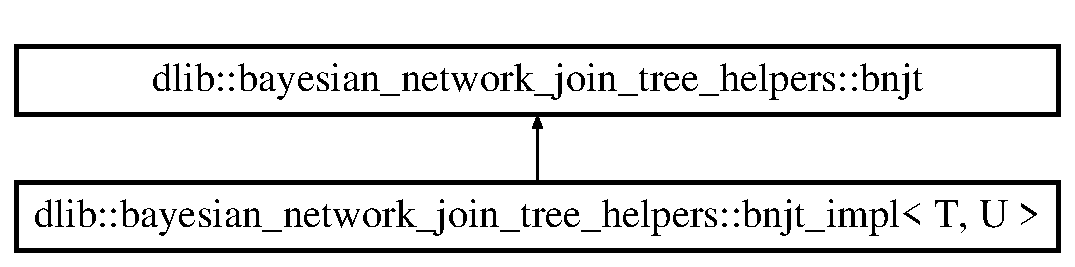
\includegraphics[height=2cm]{classdlib_1_1bayesian__network__join__tree__helpers_1_1bnjt}
\end{center}
\end{figure}
\subsection*{Public Member Functions}
\begin{DoxyCompactItemize}
\item 
virtual \hyperlink{classdlib_1_1bayesian__network__join__tree__helpers_1_1bnjt_adb02abc4db9a1dad2489a8fd9bd37a14}{$\sim$bnjt} ()
\item 
\hypertarget{classdlib_1_1bayesian__network__join__tree__helpers_1_1bnjt_a10b7f9fd3a915858faaa71b70335ec5b}{
virtual const matrix$<$ double, 1 $>$ {\bfseries probability} (unsigned long idx) const =0}
\label{classdlib_1_1bayesian__network__join__tree__helpers_1_1bnjt_a10b7f9fd3a915858faaa71b70335ec5b}

\end{DoxyCompactItemize}


\subsection{Constructor \& Destructor Documentation}
\hypertarget{classdlib_1_1bayesian__network__join__tree__helpers_1_1bnjt_adb02abc4db9a1dad2489a8fd9bd37a14}{
\index{dlib::bayesian\_\-network\_\-join\_\-tree\_\-helpers::bnjt@{dlib::bayesian\_\-network\_\-join\_\-tree\_\-helpers::bnjt}!$\sim$bnjt@{$\sim$bnjt}}
\index{$\sim$bnjt@{$\sim$bnjt}!dlib::bayesian_network_join_tree_helpers::bnjt@{dlib::bayesian\_\-network\_\-join\_\-tree\_\-helpers::bnjt}}
\subsubsection[{$\sim$bnjt}]{\setlength{\rightskip}{0pt plus 5cm}virtual dlib::bayesian\_\-network\_\-join\_\-tree\_\-helpers::bnjt::$\sim$bnjt ()\hspace{0.3cm}{\ttfamily  \mbox{[}inline, virtual\mbox{]}}}}
\label{classdlib_1_1bayesian__network__join__tree__helpers_1_1bnjt_adb02abc4db9a1dad2489a8fd9bd37a14}
this object is the base class used in this pimpl idiom ! 

The documentation for this class was generated from the following file:\begin{DoxyCompactItemize}
\item 
source/dlib/bayes\_\-utils/bayes\_\-utils.h\end{DoxyCompactItemize}

\hypertarget{classdlib_1_1bayesian__network__join__tree__helpers_1_1bnjt__impl}{
\section{dlib::bayesian\_\-network\_\-join\_\-tree\_\-helpers::bnjt\_\-impl$<$ T, U $>$ Class Template Reference}
\label{classdlib_1_1bayesian__network__join__tree__helpers_1_1bnjt__impl}\index{dlib::bayesian\_\-network\_\-join\_\-tree\_\-helpers::bnjt\_\-impl@{dlib::bayesian\_\-network\_\-join\_\-tree\_\-helpers::bnjt\_\-impl}}
}
Inheritance diagram for dlib::bayesian\_\-network\_\-join\_\-tree\_\-helpers::bnjt\_\-impl$<$ T, U $>$::\begin{figure}[H]
\begin{center}
\leavevmode
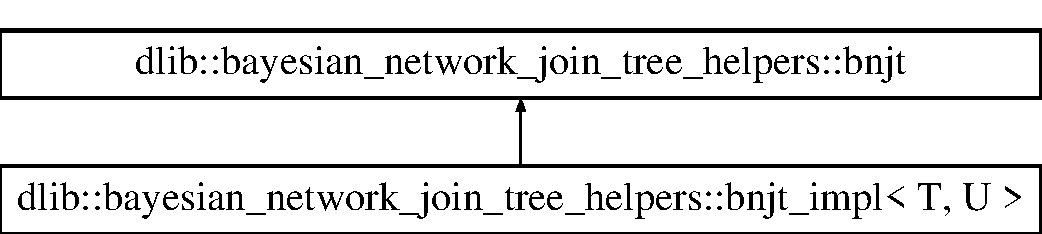
\includegraphics[height=2cm]{classdlib_1_1bayesian__network__join__tree__helpers_1_1bnjt__impl}
\end{center}
\end{figure}
\subsection*{Public Member Functions}
\begin{DoxyCompactItemize}
\item 
\hyperlink{classdlib_1_1bayesian__network__join__tree__helpers_1_1bnjt__impl_a5e845b2196c0ebddd50c919a1d62ce9a}{bnjt\_\-impl} (const T \&bn, const U \&join\_\-tree)
\item 
\hypertarget{classdlib_1_1bayesian__network__join__tree__helpers_1_1bnjt__impl_a63828a5e8f9e7501b03bc242ba276d01}{
virtual const matrix$<$ double, 1 $>$ {\bfseries probability} (unsigned long idx) const }
\label{classdlib_1_1bayesian__network__join__tree__helpers_1_1bnjt__impl_a63828a5e8f9e7501b03bc242ba276d01}

\end{DoxyCompactItemize}
\subsubsection*{template$<$typename T, typename U$>$ class dlib::bayesian\_\-network\_\-join\_\-tree\_\-helpers::bnjt\_\-impl$<$ T, U $>$}



\subsection{Constructor \& Destructor Documentation}
\hypertarget{classdlib_1_1bayesian__network__join__tree__helpers_1_1bnjt__impl_a5e845b2196c0ebddd50c919a1d62ce9a}{
\index{dlib::bayesian\_\-network\_\-join\_\-tree\_\-helpers::bnjt\_\-impl@{dlib::bayesian\_\-network\_\-join\_\-tree\_\-helpers::bnjt\_\-impl}!bnjt\_\-impl@{bnjt\_\-impl}}
\index{bnjt\_\-impl@{bnjt\_\-impl}!dlib::bayesian_network_join_tree_helpers::bnjt_impl@{dlib::bayesian\_\-network\_\-join\_\-tree\_\-helpers::bnjt\_\-impl}}
\subsubsection[{bnjt\_\-impl}]{\setlength{\rightskip}{0pt plus 5cm}template$<$typename T , typename U $>$ {\bf dlib::bayesian\_\-network\_\-join\_\-tree\_\-helpers::bnjt\_\-impl}$<$ T, U $>$::{\bf bnjt\_\-impl} (const T \& {\em bn}, \/  const U \& {\em join\_\-tree})\hspace{0.3cm}{\ttfamily  \mbox{[}inline\mbox{]}}}}
\label{classdlib_1_1bayesian__network__join__tree__helpers_1_1bnjt__impl_a5e845b2196c0ebddd50c919a1d62ce9a}
This object is the implementation in the pimpl idiom ! 

The documentation for this class was generated from the following file:\begin{DoxyCompactItemize}
\item 
source/dlib/bayes\_\-utils/bayes\_\-utils.h\end{DoxyCompactItemize}

\hypertarget{classdlib_1_1bound__function__pointer}{
\section{dlib::bound\_\-function\_\-pointer Class Reference}
\label{classdlib_1_1bound__function__pointer}\index{dlib::bound\_\-function\_\-pointer@{dlib::bound\_\-function\_\-pointer}}
}
\subsection*{Public Types}
\begin{DoxyCompactItemize}
\item 
\hypertarget{classdlib_1_1bound__function__pointer_a533e9b1ab4f8a99f21d07d28b30675b1}{
typedef bound\_\-function\_\-pointer\_\-kernel\_\-1 {\bfseries kernel\_\-1a}}
\label{classdlib_1_1bound__function__pointer_a533e9b1ab4f8a99f21d07d28b30675b1}

\item 
\hypertarget{classdlib_1_1bound__function__pointer_acb74e7ca7d63a6d0ec3cf88c4df35e5e}{
typedef bound\_\-function\_\-pointer\_\-kernel\_\-c$<$ kernel\_\-1a $>$ {\bfseries kernel\_\-1a\_\-c}}
\label{classdlib_1_1bound__function__pointer_acb74e7ca7d63a6d0ec3cf88c4df35e5e}

\end{DoxyCompactItemize}


The documentation for this class was generated from the following file:\begin{DoxyCompactItemize}
\item 
source/dlib/bound\_\-function\_\-pointer.h\end{DoxyCompactItemize}

\hypertarget{classdlib_1_1byte__orderer}{
\section{dlib::byte\_\-orderer Class Reference}
\label{classdlib_1_1byte__orderer}\index{dlib::byte\_\-orderer@{dlib::byte\_\-orderer}}
}
\subsection*{Public Types}
\begin{DoxyCompactItemize}
\item 
\hypertarget{classdlib_1_1byte__orderer_aae9fdefa43755bb52b75f7a924f12737}{
typedef byte\_\-orderer\_\-kernel\_\-1 {\bfseries kernel\_\-1a}}
\label{classdlib_1_1byte__orderer_aae9fdefa43755bb52b75f7a924f12737}

\end{DoxyCompactItemize}


The documentation for this class was generated from the following file:\begin{DoxyCompactItemize}
\item 
source/dlib/byte\_\-orderer.h\end{DoxyCompactItemize}

\hypertarget{classdlib_1_1cmd__line__parser}{
\section{dlib::cmd\_\-line\_\-parser$<$ charT $>$ Class Template Reference}
\label{classdlib_1_1cmd__line__parser}\index{dlib::cmd\_\-line\_\-parser@{dlib::cmd\_\-line\_\-parser}}
}
\subsection*{Public Types}
\begin{DoxyCompactItemize}
\item 
\hypertarget{classdlib_1_1cmd__line__parser_a5b27a4d9d3a074860a7bfc57d85f1d32}{
typedef cmd\_\-line\_\-parser\_\-kernel\_\-1$<$ charT, map\_\-1a\_\-string, sequence\_\-2a, psequence\_\-2a $>$ {\bfseries kernel\_\-1a}}
\label{classdlib_1_1cmd__line__parser_a5b27a4d9d3a074860a7bfc57d85f1d32}

\item 
\hypertarget{classdlib_1_1cmd__line__parser_a38a8f350b37b240cbe79ef1e69afc0fd}{
typedef cmd\_\-line\_\-parser\_\-kernel\_\-c$<$ kernel\_\-1a $>$ {\bfseries kernel\_\-1a\_\-c}}
\label{classdlib_1_1cmd__line__parser_a38a8f350b37b240cbe79ef1e69afc0fd}

\item 
\hypertarget{classdlib_1_1cmd__line__parser_a061a11289be9d6b9d0ba4791608ce2f5}{
typedef cmd\_\-line\_\-parser\_\-print\_\-1$<$ kernel\_\-1a $>$ {\bfseries print\_\-1a}}
\label{classdlib_1_1cmd__line__parser_a061a11289be9d6b9d0ba4791608ce2f5}

\item 
\hypertarget{classdlib_1_1cmd__line__parser_a092fed2a65b5e25ae36dfdc875e59ee4}{
typedef cmd\_\-line\_\-parser\_\-print\_\-1$<$ kernel\_\-1a\_\-c $>$ {\bfseries print\_\-1a\_\-c}}
\label{classdlib_1_1cmd__line__parser_a092fed2a65b5e25ae36dfdc875e59ee4}

\item 
\hypertarget{classdlib_1_1cmd__line__parser_a028842bc91b63086a31bdafce3576586}{
typedef cmd\_\-line\_\-parser\_\-check\_\-1$<$ print\_\-1a $>$ {\bfseries check\_\-1a}}
\label{classdlib_1_1cmd__line__parser_a028842bc91b63086a31bdafce3576586}

\item 
\hypertarget{classdlib_1_1cmd__line__parser_af9221ba7331710e527346c7368ee5628}{
typedef cmd\_\-line\_\-parser\_\-check\_\-c$<$ cmd\_\-line\_\-parser\_\-check\_\-1$<$ print\_\-1a\_\-c $>$ $>$ {\bfseries check\_\-1a\_\-c}}
\label{classdlib_1_1cmd__line__parser_af9221ba7331710e527346c7368ee5628}

\end{DoxyCompactItemize}
\subsubsection*{template$<$typename charT$>$ class dlib::cmd\_\-line\_\-parser$<$ charT $>$}



The documentation for this class was generated from the following file:\begin{DoxyCompactItemize}
\item 
source/dlib/cmd\_\-line\_\-parser.h\end{DoxyCompactItemize}

\hypertarget{structdlib_1_1assign__pixel__helpers_1_1COLOUR}{
\section{dlib::assign\_\-pixel\_\-helpers::COLOUR Struct Reference}
\label{structdlib_1_1assign__pixel__helpers_1_1COLOUR}\index{dlib::assign\_\-pixel\_\-helpers::COLOUR@{dlib::assign\_\-pixel\_\-helpers::COLOUR}}
}
\subsection*{Public Attributes}
\begin{DoxyCompactItemize}
\item 
\hypertarget{structdlib_1_1assign__pixel__helpers_1_1COLOUR_af2e26a1ed3dac0e6ae25684de1e2c408}{
double {\bfseries r}}
\label{structdlib_1_1assign__pixel__helpers_1_1COLOUR_af2e26a1ed3dac0e6ae25684de1e2c408}

\item 
\hypertarget{structdlib_1_1assign__pixel__helpers_1_1COLOUR_ab9df6f2551a9b3cae245c7cfb8ebb3e5}{
double {\bfseries g}}
\label{structdlib_1_1assign__pixel__helpers_1_1COLOUR_ab9df6f2551a9b3cae245c7cfb8ebb3e5}

\item 
\hypertarget{structdlib_1_1assign__pixel__helpers_1_1COLOUR_af289608c223577fef437a8d6a05e653b}{
double {\bfseries b}}
\label{structdlib_1_1assign__pixel__helpers_1_1COLOUR_af289608c223577fef437a8d6a05e653b}

\end{DoxyCompactItemize}


The documentation for this struct was generated from the following file:\begin{DoxyCompactItemize}
\item 
source/dlib/pixel.h\end{DoxyCompactItemize}

\hypertarget{structdlib_1_1compile__time__assert_3_01true_01_4}{
\section{dlib::compile\_\-time\_\-assert$<$ true $>$ Struct Template Reference}
\label{structdlib_1_1compile__time__assert_3_01true_01_4}\index{dlib::compile\_\-time\_\-assert$<$ true $>$@{dlib::compile\_\-time\_\-assert$<$ true $>$}}
}
\subsection*{Public Types}
\begin{DoxyCompactItemize}
\item 
enum \{ {\bfseries value} = 1
 \}
\end{DoxyCompactItemize}
\subsubsection*{template$<$$>$ struct dlib::compile\_\-time\_\-assert$<$ true $>$}



The documentation for this struct was generated from the following file:\begin{DoxyCompactItemize}
\item 
source/dlib/assert.h\end{DoxyCompactItemize}

\hypertarget{classdlib_1_1compress__stream}{
\section{dlib::compress\_\-stream Class Reference}
\label{classdlib_1_1compress__stream}\index{dlib::compress\_\-stream@{dlib::compress\_\-stream}}
}
\subsection*{Public Types}
\begin{DoxyCompactItemize}
\item 
\hypertarget{classdlib_1_1compress__stream_a7ac38313ebb877bf19451de0c0380d0f}{
typedef compress\_\-stream\_\-kernel\_\-1$<$ fce1, fcd1, crc32::kernel\_\-1a $>$ {\bfseries kernel\_\-1a}}
\label{classdlib_1_1compress__stream_a7ac38313ebb877bf19451de0c0380d0f}

\item 
\hypertarget{classdlib_1_1compress__stream_a7fb1453dd170b9e3898d428b9a96f62a}{
typedef compress\_\-stream\_\-kernel\_\-1$<$ fce2, fcd2, crc32::kernel\_\-1a $>$ {\bfseries kernel\_\-1b}}
\label{classdlib_1_1compress__stream_a7fb1453dd170b9e3898d428b9a96f62a}

\item 
\hypertarget{classdlib_1_1compress__stream_afaa6401526a71d7a9ca30ee995839264}{
typedef compress\_\-stream\_\-kernel\_\-1$<$ fce3, fcd3, crc32::kernel\_\-1a $>$ {\bfseries kernel\_\-1c}}
\label{classdlib_1_1compress__stream_afaa6401526a71d7a9ca30ee995839264}

\item 
\hypertarget{classdlib_1_1compress__stream_a950476085b35dffd63b5413c33d19c55}{
typedef compress\_\-stream\_\-kernel\_\-1$<$ fce4a, fcd4a, crc32::kernel\_\-1a $>$ {\bfseries kernel\_\-1da}}
\label{classdlib_1_1compress__stream_a950476085b35dffd63b5413c33d19c55}

\item 
\hypertarget{classdlib_1_1compress__stream_a59ed7ead43813f0a7bce882820a60692}{
typedef compress\_\-stream\_\-kernel\_\-1$<$ fce5a, fcd5a, crc32::kernel\_\-1a $>$ {\bfseries kernel\_\-1ea}}
\label{classdlib_1_1compress__stream_a59ed7ead43813f0a7bce882820a60692}

\item 
\hypertarget{classdlib_1_1compress__stream_ac8581a6a7014934197c7f50f66459fc4}{
typedef compress\_\-stream\_\-kernel\_\-1$<$ fce4b, fcd4b, crc32::kernel\_\-1a $>$ {\bfseries kernel\_\-1db}}
\label{classdlib_1_1compress__stream_ac8581a6a7014934197c7f50f66459fc4}

\item 
\hypertarget{classdlib_1_1compress__stream_a8e201dfafbdbbc84f27160b63a3d71e4}{
typedef compress\_\-stream\_\-kernel\_\-1$<$ fce5b, fcd5b, crc32::kernel\_\-1a $>$ {\bfseries kernel\_\-1eb}}
\label{classdlib_1_1compress__stream_a8e201dfafbdbbc84f27160b63a3d71e4}

\item 
\hypertarget{classdlib_1_1compress__stream_ae4e15b8daac13f85d03903e788266476}{
typedef compress\_\-stream\_\-kernel\_\-1$<$ fce5c, fcd5c, crc32::kernel\_\-1a $>$ {\bfseries kernel\_\-1ec}}
\label{classdlib_1_1compress__stream_ae4e15b8daac13f85d03903e788266476}

\item 
\hypertarget{classdlib_1_1compress__stream_ae84be8fae8af9200083ca33d2e2bdd61}{
typedef compress\_\-stream\_\-kernel\_\-2$<$ fce2, fcd2, lz77\_\-buffer2a, sliding\_\-buffer1, fce\_\-length, fcd\_\-length, fce\_\-index, fcd\_\-index, crc32::kernel\_\-1a $>$ {\bfseries kernel\_\-2a}}
\label{classdlib_1_1compress__stream_ae84be8fae8af9200083ca33d2e2bdd61}

\item 
\hypertarget{classdlib_1_1compress__stream_a0940b332f05ad0172f55c9925e9187f1}{
typedef compress\_\-stream\_\-kernel\_\-3$<$ lzp\_\-buf\_\-1, crc32::kernel\_\-1a, 16 $>$ {\bfseries kernel\_\-3a}}
\label{classdlib_1_1compress__stream_a0940b332f05ad0172f55c9925e9187f1}

\item 
\hypertarget{classdlib_1_1compress__stream_aed651926e16d3f77d659e116f09baf4d}{
typedef compress\_\-stream\_\-kernel\_\-3$<$ lzp\_\-buf\_\-2, crc32::kernel\_\-1a, 16 $>$ {\bfseries kernel\_\-3b}}
\label{classdlib_1_1compress__stream_aed651926e16d3f77d659e116f09baf4d}

\end{DoxyCompactItemize}


The documentation for this class was generated from the following file:\begin{DoxyCompactItemize}
\item 
source/dlib/compress\_\-stream.h\end{DoxyCompactItemize}

\hypertarget{classdlib_1_1conditional__probability__table}{
\section{dlib::conditional\_\-probability\_\-table Class Reference}
\label{classdlib_1_1conditional__probability__table}\index{dlib::conditional\_\-probability\_\-table@{dlib::conditional\_\-probability\_\-table}}
}


Inherits boost::noncopyable.\subsection*{Public Member Functions}
\begin{DoxyCompactItemize}
\item 
\hyperlink{classdlib_1_1conditional__probability__table_a0b0989c283746263c7f339f10da7b59e}{conditional\_\-probability\_\-table} ()
\item 
\hypertarget{classdlib_1_1conditional__probability__table_a3ffa4aa9ba7bb1eabf149f2a79cf36cb}{
void {\bfseries set\_\-num\_\-values} (unsigned long num)}
\label{classdlib_1_1conditional__probability__table_a3ffa4aa9ba7bb1eabf149f2a79cf36cb}

\item 
\hypertarget{classdlib_1_1conditional__probability__table_aa90e4a805f3681b5827d61f9fd8008eb}{
bool {\bfseries has\_\-entry\_\-for} (unsigned long value, const \hyperlink{classdlib_1_1assignment}{assignment} \&ps) const }
\label{classdlib_1_1conditional__probability__table_aa90e4a805f3681b5827d61f9fd8008eb}

\item 
\hypertarget{classdlib_1_1conditional__probability__table_a7d8e2b5658bb4a4822cc8ca907549491}{
unsigned long {\bfseries num\_\-values} () const }
\label{classdlib_1_1conditional__probability__table_a7d8e2b5658bb4a4822cc8ca907549491}

\item 
\hypertarget{classdlib_1_1conditional__probability__table_a3ebb76d3b0897f1680c452f2773a03c4}{
void {\bfseries set\_\-probability} (unsigned long value, const \hyperlink{classdlib_1_1assignment}{assignment} \&ps, double p)}
\label{classdlib_1_1conditional__probability__table_a3ebb76d3b0897f1680c452f2773a03c4}

\item 
\hypertarget{classdlib_1_1conditional__probability__table_a62071a87ac8c6d5615e805069347efd7}{
double {\bfseries probability} (unsigned long value, const \hyperlink{classdlib_1_1assignment}{assignment} \&ps) const }
\label{classdlib_1_1conditional__probability__table_a62071a87ac8c6d5615e805069347efd7}

\item 
\hypertarget{classdlib_1_1conditional__probability__table_a8609aeb4e06ec372ab4631a86be70301}{
void {\bfseries clear} ()}
\label{classdlib_1_1conditional__probability__table_a8609aeb4e06ec372ab4631a86be70301}

\item 
\hypertarget{classdlib_1_1conditional__probability__table_a873e1d843be718dbd19005efeaa7d0a3}{
void {\bfseries empty\_\-table} ()}
\label{classdlib_1_1conditional__probability__table_a873e1d843be718dbd19005efeaa7d0a3}

\item 
\hypertarget{classdlib_1_1conditional__probability__table_a684f81ed409334eebf7e492067831d22}{
void {\bfseries swap} (\hyperlink{classdlib_1_1conditional__probability__table}{conditional\_\-probability\_\-table} \&item)}
\label{classdlib_1_1conditional__probability__table_a684f81ed409334eebf7e492067831d22}

\end{DoxyCompactItemize}
\subsection*{Friends}
\begin{DoxyCompactItemize}
\item 
\hypertarget{classdlib_1_1conditional__probability__table_a0080cd288987dd9aece2b6dd654ca0cd}{
void {\bfseries serialize} (const \hyperlink{classdlib_1_1conditional__probability__table}{conditional\_\-probability\_\-table} \&item, std::ostream \&out)}
\label{classdlib_1_1conditional__probability__table_a0080cd288987dd9aece2b6dd654ca0cd}

\item 
\hypertarget{classdlib_1_1conditional__probability__table_aee97c3b0a890ea640ee7ba7b80632041}{
void {\bfseries deserialize} (\hyperlink{classdlib_1_1conditional__probability__table}{conditional\_\-probability\_\-table} \&item, std::istream \&in)}
\label{classdlib_1_1conditional__probability__table_aee97c3b0a890ea640ee7ba7b80632041}

\end{DoxyCompactItemize}


\subsection{Constructor \& Destructor Documentation}
\hypertarget{classdlib_1_1conditional__probability__table_a0b0989c283746263c7f339f10da7b59e}{
\index{dlib::conditional\_\-probability\_\-table@{dlib::conditional\_\-probability\_\-table}!conditional\_\-probability\_\-table@{conditional\_\-probability\_\-table}}
\index{conditional\_\-probability\_\-table@{conditional\_\-probability\_\-table}!dlib::conditional_probability_table@{dlib::conditional\_\-probability\_\-table}}
\subsubsection[{conditional\_\-probability\_\-table}]{\setlength{\rightskip}{0pt plus 5cm}dlib::conditional\_\-probability\_\-table::conditional\_\-probability\_\-table ()\hspace{0.3cm}{\ttfamily  \mbox{[}inline\mbox{]}}}}
\label{classdlib_1_1conditional__probability__table_a0b0989c283746263c7f339f10da7b59e}
INITIAL VALUE
\begin{DoxyItemize}
\item table.size() == 0
\end{DoxyItemize}

CONVENTION
\begin{DoxyItemize}
\item if (table.is\_\-in\_\-domain(ps) \&\& value $<$ num\_\-vals \&\& table\mbox{[}ps\mbox{]}(value) $>$= 0) then
\begin{DoxyItemize}
\item has\_\-entry\_\-for(value,ps) == true
\item probability(value,ps) == table\mbox{[}ps\mbox{]}(value)
\end{DoxyItemize}
\item else
\begin{DoxyItemize}
\item has\_\-entry\_\-for(value,ps) == false
\end{DoxyItemize}
\end{DoxyItemize}


\begin{DoxyItemize}
\item num\_\-values() == num\_\-vals ! 
\end{DoxyItemize}

The documentation for this class was generated from the following file:\begin{DoxyCompactItemize}
\item 
source/dlib/bayes\_\-utils/bayes\_\-utils.h\end{DoxyCompactItemize}

\hypertarget{classdlib_1_1conditioning__class}{
\section{dlib::conditioning\_\-class$<$ alphabet\_\-size $>$ Class Template Reference}
\label{classdlib_1_1conditioning__class}\index{dlib::conditioning\_\-class@{dlib::conditioning\_\-class}}
}
\subsection*{Public Types}
\begin{DoxyCompactItemize}
\item 
\hypertarget{classdlib_1_1conditioning__class_a2aa10e4625308ec0f112bc9cab1a87b4}{
typedef conditioning\_\-class\_\-kernel\_\-1$<$ alphabet\_\-size $>$ {\bfseries kernel\_\-1a}}
\label{classdlib_1_1conditioning__class_a2aa10e4625308ec0f112bc9cab1a87b4}

\item 
\hypertarget{classdlib_1_1conditioning__class_ad77a44016d35a2d50301b8fcdb1d7e76}{
typedef conditioning\_\-class\_\-kernel\_\-c$<$ kernel\_\-1a $>$ {\bfseries kernel\_\-1a\_\-c}}
\label{classdlib_1_1conditioning__class_ad77a44016d35a2d50301b8fcdb1d7e76}

\item 
\hypertarget{classdlib_1_1conditioning__class_a41fbf8cd6b4a34869f3cbc38ce14e937}{
typedef conditioning\_\-class\_\-kernel\_\-2$<$ alphabet\_\-size $>$ {\bfseries kernel\_\-2a}}
\label{classdlib_1_1conditioning__class_a41fbf8cd6b4a34869f3cbc38ce14e937}

\item 
\hypertarget{classdlib_1_1conditioning__class_a497e0c7e3d950b6488c3e6458270cd7f}{
typedef conditioning\_\-class\_\-kernel\_\-c$<$ kernel\_\-2a $>$ {\bfseries kernel\_\-2a\_\-c}}
\label{classdlib_1_1conditioning__class_a497e0c7e3d950b6488c3e6458270cd7f}

\item 
\hypertarget{classdlib_1_1conditioning__class_ac3ab6a7ed69f658386add2247017554f}{
typedef conditioning\_\-class\_\-kernel\_\-3$<$ alphabet\_\-size $>$ {\bfseries kernel\_\-3a}}
\label{classdlib_1_1conditioning__class_ac3ab6a7ed69f658386add2247017554f}

\item 
\hypertarget{classdlib_1_1conditioning__class_a2b7be95af893b328128c5f11fb0870c6}{
typedef conditioning\_\-class\_\-kernel\_\-c$<$ kernel\_\-3a $>$ {\bfseries kernel\_\-3a\_\-c}}
\label{classdlib_1_1conditioning__class_a2b7be95af893b328128c5f11fb0870c6}

\item 
\hypertarget{classdlib_1_1conditioning__class_a2752541f8fb95e288c4922356a128ef4}{
typedef conditioning\_\-class\_\-kernel\_\-4$<$ alphabet\_\-size, 10000, mm $>$ {\bfseries kernel\_\-4a}}
\label{classdlib_1_1conditioning__class_a2752541f8fb95e288c4922356a128ef4}

\item 
\hypertarget{classdlib_1_1conditioning__class_aa06d63b281e56242af65aa990cc48730}{
typedef conditioning\_\-class\_\-kernel\_\-c$<$ kernel\_\-4a $>$ {\bfseries kernel\_\-4a\_\-c}}
\label{classdlib_1_1conditioning__class_aa06d63b281e56242af65aa990cc48730}

\item 
\hypertarget{classdlib_1_1conditioning__class_a661af4f352d54171ff603faf20569031}{
typedef conditioning\_\-class\_\-kernel\_\-4$<$ alphabet\_\-size, 100000, mm $>$ {\bfseries kernel\_\-4b}}
\label{classdlib_1_1conditioning__class_a661af4f352d54171ff603faf20569031}

\item 
\hypertarget{classdlib_1_1conditioning__class_aee6cf5b7f0e5155b50c8619919597330}{
typedef conditioning\_\-class\_\-kernel\_\-c$<$ kernel\_\-4b $>$ {\bfseries kernel\_\-4b\_\-c}}
\label{classdlib_1_1conditioning__class_aee6cf5b7f0e5155b50c8619919597330}

\item 
\hypertarget{classdlib_1_1conditioning__class_a09300657f2de500c9756ac44cc55d395}{
typedef conditioning\_\-class\_\-kernel\_\-4$<$ alphabet\_\-size, 1000000, mm $>$ {\bfseries kernel\_\-4c}}
\label{classdlib_1_1conditioning__class_a09300657f2de500c9756ac44cc55d395}

\item 
\hypertarget{classdlib_1_1conditioning__class_aaa49dd0ab67b10e33d7c7d33777075a9}{
typedef conditioning\_\-class\_\-kernel\_\-c$<$ kernel\_\-4c $>$ {\bfseries kernel\_\-4c\_\-c}}
\label{classdlib_1_1conditioning__class_aaa49dd0ab67b10e33d7c7d33777075a9}

\item 
\hypertarget{classdlib_1_1conditioning__class_aea6478d0c4d6b20179c495f7bf4286ce}{
typedef conditioning\_\-class\_\-kernel\_\-4$<$ alphabet\_\-size, 10000000, mm $>$ {\bfseries kernel\_\-4d}}
\label{classdlib_1_1conditioning__class_aea6478d0c4d6b20179c495f7bf4286ce}

\item 
\hypertarget{classdlib_1_1conditioning__class_aeda54b2b0bd3e3c8bbe6fa4746786193}{
typedef conditioning\_\-class\_\-kernel\_\-c$<$ kernel\_\-4d $>$ {\bfseries kernel\_\-4d\_\-c}}
\label{classdlib_1_1conditioning__class_aeda54b2b0bd3e3c8bbe6fa4746786193}

\end{DoxyCompactItemize}
\subsubsection*{template$<$unsigned long alphabet\_\-size$>$ class dlib::conditioning\_\-class$<$ alphabet\_\-size $>$}



The documentation for this class was generated from the following file:\begin{DoxyCompactItemize}
\item 
source/dlib/conditioning\_\-class.h\end{DoxyCompactItemize}

\hypertarget{classdlib_1_1config__reader}{
\section{dlib::config\_\-reader Class Reference}
\label{classdlib_1_1config__reader}\index{dlib::config\_\-reader@{dlib::config\_\-reader}}
}
\subsection*{Public Types}
\begin{DoxyCompactItemize}
\item 
\hypertarget{classdlib_1_1config__reader_a98434e74d8584f650cfc382922bbbb08}{
typedef config\_\-reader\_\-kernel\_\-1$<$ \hyperlink{classdlib_1_1map}{map}$<$ std::string, std::string $>$::kernel\_\-1b, \hyperlink{classdlib_1_1map}{map}$<$ std::string, void $\ast$ $>$::kernel\_\-1b, tokenizer::kernel\_\-1a $>$ {\bfseries kernel\_\-1a}}
\label{classdlib_1_1config__reader_a98434e74d8584f650cfc382922bbbb08}

\item 
\hypertarget{classdlib_1_1config__reader_a202da19d39f9c6b1799796849637458f}{
typedef config\_\-reader\_\-thread\_\-safe\_\-1$<$ kernel\_\-1a, \hyperlink{classdlib_1_1map}{map}$<$ std::string, void $\ast$ $>$::kernel\_\-1b $>$ {\bfseries thread\_\-safe\_\-1a}}
\label{classdlib_1_1config__reader_a202da19d39f9c6b1799796849637458f}

\end{DoxyCompactItemize}


The documentation for this class was generated from the following file:\begin{DoxyCompactItemize}
\item 
source/dlib/config\_\-reader.h\end{DoxyCompactItemize}

\hypertarget{classdlib_1_1copy__functor}{
\section{dlib::copy\_\-functor$<$ T $>$ Class Template Reference}
\label{classdlib_1_1copy__functor}\index{dlib::copy\_\-functor@{dlib::copy\_\-functor}}
}
\subsection*{Public Member Functions}
\begin{DoxyCompactItemize}
\item 
\hypertarget{classdlib_1_1copy__functor_a508324ae27d9d1675714f3f95e93b2ec}{
void {\bfseries operator()} (const T \&source, T \&destination) const }
\label{classdlib_1_1copy__functor_a508324ae27d9d1675714f3f95e93b2ec}

\end{DoxyCompactItemize}
\subsubsection*{template$<$typename T$>$ class dlib::copy\_\-functor$<$ T $>$}



The documentation for this class was generated from the following file:\begin{DoxyCompactItemize}
\item 
source/dlib/algs.h\end{DoxyCompactItemize}

\hypertarget{classdlib_1_1cpp__pretty__printer}{
\section{dlib::cpp\_\-pretty\_\-printer Class Reference}
\label{classdlib_1_1cpp__pretty__printer}\index{dlib::cpp\_\-pretty\_\-printer@{dlib::cpp\_\-pretty\_\-printer}}
}
\subsection*{Public Types}
\begin{DoxyCompactItemize}
\item 
\hypertarget{classdlib_1_1cpp__pretty__printer_a990595778cddb7e3683a1643663f0605}{
typedef cpp\_\-pretty\_\-printer\_\-kernel\_\-1$<$ \hyperlink{classdlib_1_1stack}{stack}, tok $>$ {\bfseries kernel\_\-1a}}
\label{classdlib_1_1cpp__pretty__printer_a990595778cddb7e3683a1643663f0605}

\item 
\hypertarget{classdlib_1_1cpp__pretty__printer_a6f68d38cc9db1c5b82158044c4fbd96e}{
typedef cpp\_\-pretty\_\-printer\_\-kernel\_\-2$<$ \hyperlink{classdlib_1_1stack}{stack}, tok $>$ {\bfseries kernel\_\-2a}}
\label{classdlib_1_1cpp__pretty__printer_a6f68d38cc9db1c5b82158044c4fbd96e}

\end{DoxyCompactItemize}


The documentation for this class was generated from the following file:\begin{DoxyCompactItemize}
\item 
source/dlib/cpp\_\-pretty\_\-printer.h\end{DoxyCompactItemize}

\hypertarget{classdlib_1_1cpp__tokenizer}{
\section{dlib::cpp\_\-tokenizer Class Reference}
\label{classdlib_1_1cpp__tokenizer}\index{dlib::cpp\_\-tokenizer@{dlib::cpp\_\-tokenizer}}
}
\subsection*{Public Types}
\begin{DoxyCompactItemize}
\item 
\hypertarget{classdlib_1_1cpp__tokenizer_aeb168845b30615d7d8357e3eb315cf33}{
typedef cpp\_\-tokenizer\_\-kernel\_\-1$<$ tok, \hyperlink{classdlib_1_1queue}{queue}, \hyperlink{classdlib_1_1set}{set} $>$ {\bfseries kernel\_\-1a}}
\label{classdlib_1_1cpp__tokenizer_aeb168845b30615d7d8357e3eb315cf33}

\item 
\hypertarget{classdlib_1_1cpp__tokenizer_a2221cf04db85bd58335601bd6ddd2cc7}{
typedef cpp\_\-tokenizer\_\-kernel\_\-c$<$ kernel\_\-1a $>$ {\bfseries kernel\_\-1a\_\-c}}
\label{classdlib_1_1cpp__tokenizer_a2221cf04db85bd58335601bd6ddd2cc7}

\end{DoxyCompactItemize}


The documentation for this class was generated from the following file:\begin{DoxyCompactItemize}
\item 
source/dlib/cpp\_\-tokenizer.h\end{DoxyCompactItemize}

\hypertarget{classdlib_1_1crc32}{
\section{dlib::crc32 Class Reference}
\label{classdlib_1_1crc32}\index{dlib::crc32@{dlib::crc32}}
}
\subsection*{Public Types}
\begin{DoxyCompactItemize}
\item 
\hypertarget{classdlib_1_1crc32_ad29669d6f6595828c30aee9244ec6f91}{
typedef crc32\_\-kernel\_\-1 {\bfseries kernel\_\-1a}}
\label{classdlib_1_1crc32_ad29669d6f6595828c30aee9244ec6f91}

\end{DoxyCompactItemize}


The documentation for this class was generated from the following file:\begin{DoxyCompactItemize}
\item 
source/dlib/crc32.h\end{DoxyCompactItemize}

\hypertarget{classDecision}{
\section{Decision Class Reference}
\label{classDecision}\index{Decision@{Decision}}
}
\subsection*{Public Member Functions}
\begin{DoxyCompactItemize}
\item 
\hypertarget{classDecision_a7b8d8d0b3afb1ac36398d062118f6d6b}{
{\bfseries Decision} (\hyperlink{classPlot}{Plot} $\ast$, const CL\_\-DomElement \&)}
\label{classDecision_a7b8d8d0b3afb1ac36398d062118f6d6b}

\item 
\hypertarget{classDecision_ae6d6d18b9890c8706bd5986978be69b6}{
CL\_\-String {\bfseries getResultAsString} (void)}
\label{classDecision_ae6d6d18b9890c8706bd5986978be69b6}

\item 
\hypertarget{classDecision_a76817bb860641012831b8d5d7857562a}{
int {\bfseries getResultAsInteger} (void)}
\label{classDecision_a76817bb860641012831b8d5d7857562a}

\item 
\hypertarget{classDecision_a8ad5b405e0f154ffe064cb4f548b7931}{
double {\bfseries getResultAsDouble} (void)}
\label{classDecision_a8ad5b405e0f154ffe064cb4f548b7931}

\item 
CL\_\-String \hyperlink{classDecision_a3b4bc70a203e47be88bfdb6d5e059ffb}{getResultType} (void)
\end{DoxyCompactItemize}


\subsection{Member Function Documentation}
\hypertarget{classDecision_a3b4bc70a203e47be88bfdb6d5e059ffb}{
\index{Decision@{Decision}!getResultType@{getResultType}}
\index{getResultType@{getResultType}!Decision@{Decision}}
\subsubsection[{getResultType}]{\setlength{\rightskip}{0pt plus 5cm}CL\_\-String Decision::getResultType (void)}}
\label{classDecision_a3b4bc70a203e47be88bfdb6d5e059ffb}
Returns the type of the value as a string. 

The documentation for this class was generated from the following files:\begin{DoxyCompactItemize}
\item 
source/mystery\_\-xml/Decision.h\item 
source/mystery\_\-xml/Decision.cpp\end{DoxyCompactItemize}

\hypertarget{classDecisions}{
\section{Decisions Class Reference}
\label{classDecisions}\index{Decisions@{Decisions}}
}
\subsection*{Public Member Functions}
\begin{DoxyCompactItemize}
\item 
\hypertarget{classDecisions_a8c89d9f293fd2a70a4c1509a60986382}{
{\bfseries Decisions} (\hyperlink{classPlot}{Plot} $\ast$, const CL\_\-DomElement \&)}
\label{classDecisions_a8c89d9f293fd2a70a4c1509a60986382}

\end{DoxyCompactItemize}


The documentation for this class was generated from the following files:\begin{DoxyCompactItemize}
\item 
source/mystery\_\-xml/\hyperlink{Decisions_8h}{Decisions.h}\item 
source/mystery\_\-xml/\hyperlink{Decisions_8cpp}{Decisions.cpp}\end{DoxyCompactItemize}

\hypertarget{structdlib_1_1default__is__kind__value}{
\section{dlib::default\_\-is\_\-kind\_\-value Struct Reference}
\label{structdlib_1_1default__is__kind__value}\index{dlib::default\_\-is\_\-kind\_\-value@{dlib::default\_\-is\_\-kind\_\-value}}
}


{\ttfamily \#include $<$is\_\-kind.h$>$}Inheritance diagram for dlib::default\_\-is\_\-kind\_\-value::\begin{figure}[H]
\begin{center}
\leavevmode
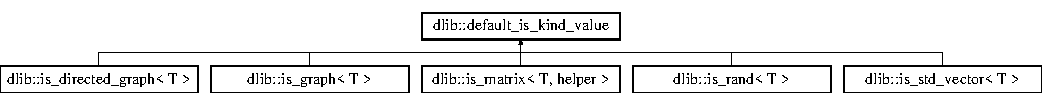
\includegraphics[height=1.2514cm]{structdlib_1_1default__is__kind__value}
\end{center}
\end{figure}
\subsection*{Static Public Attributes}
\begin{DoxyCompactItemize}
\item 
\hypertarget{structdlib_1_1default__is__kind__value_a64fbc73b0365a73a09f76b9ee31f60a8}{
static const bool {\bfseries value} = false}
\label{structdlib_1_1default__is__kind__value_a64fbc73b0365a73a09f76b9ee31f60a8}

\end{DoxyCompactItemize}


\subsection{Detailed Description}
This file contains a \hyperlink{classdlib_1_1set}{set} of templates that enable you to determine if a given type implements an abstract interface defined in one of the \hyperlink{namespacedlib}{dlib} $\ast$\_\-abstract.h files. ! 

The documentation for this struct was generated from the following file:\begin{DoxyCompactItemize}
\item 
source/dlib/is\_\-kind.h\end{DoxyCompactItemize}

\hypertarget{classdlib_1_1directed__graph}{
\section{dlib::directed\_\-graph$<$ T, E, mem\_\-manager $>$ Class Template Reference}
\label{classdlib_1_1directed__graph}\index{dlib::directed\_\-graph@{dlib::directed\_\-graph}}
}
\subsection*{Public Types}
\begin{DoxyCompactItemize}
\item 
\hypertarget{classdlib_1_1directed__graph_a65ce21ff3926ab6c85a17ecec725aa77}{
typedef directed\_\-graph\_\-kernel\_\-1$<$ T, E, mem\_\-manager, false $>$ {\bfseries kernel\_\-1a}}
\label{classdlib_1_1directed__graph_a65ce21ff3926ab6c85a17ecec725aa77}

\item 
\hypertarget{classdlib_1_1directed__graph_a80c78956bd7695021e8a60a872467fbd}{
typedef directed\_\-graph\_\-kernel\_\-1$<$ T, E, mem\_\-manager, true $>$ {\bfseries kernel\_\-1a\_\-c}}
\label{classdlib_1_1directed__graph_a80c78956bd7695021e8a60a872467fbd}

\end{DoxyCompactItemize}
\subsubsection*{template$<$typename T, typename E = char, typename mem\_\-manager = memory\_\-manager$<$char$>$::kernel\_\-1a$>$ class dlib::directed\_\-graph$<$ T, E, mem\_\-manager $>$}



The documentation for this class was generated from the following file:\begin{DoxyCompactItemize}
\item 
source/dlib/directed\_\-graph.h\end{DoxyCompactItemize}

\hypertarget{structboost_1_1disable__if}{
\section{boost::disable\_\-if$<$ Cond, T $>$ Struct Template Reference}
\label{structboost_1_1disable__if}\index{boost::disable\_\-if@{boost::disable\_\-if}}
}
Inheritance diagram for boost::disable\_\-if$<$ Cond, T $>$::\begin{figure}[H]
\begin{center}
\leavevmode
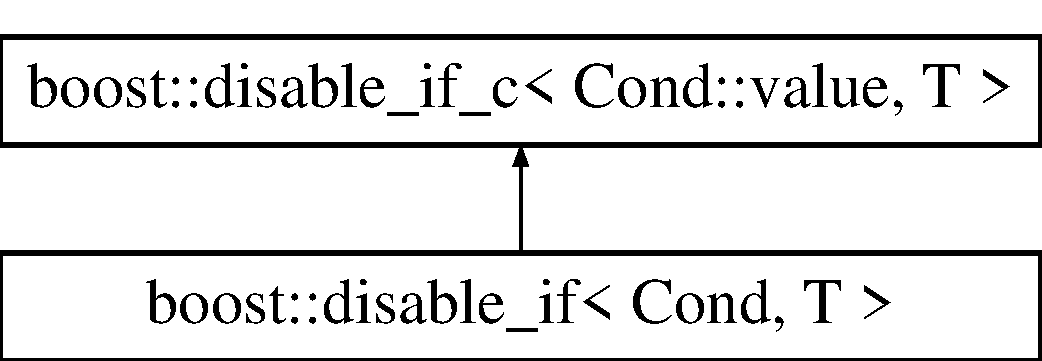
\includegraphics[height=2cm]{structboost_1_1disable__if}
\end{center}
\end{figure}
\subsubsection*{template$<$class Cond, class T = void$>$ struct boost::disable\_\-if$<$ Cond, T $>$}



The documentation for this struct was generated from the following file:\begin{DoxyCompactItemize}
\item 
source/dlib/enable\_\-if.h\end{DoxyCompactItemize}

\hypertarget{structboost_1_1disable__if__c}{
\section{boost::disable\_\-if\_\-c$<$ B, T $>$ Struct Template Reference}
\label{structboost_1_1disable__if__c}\index{boost::disable\_\-if\_\-c@{boost::disable\_\-if\_\-c}}
}
\subsection*{Public Types}
\begin{DoxyCompactItemize}
\item 
\hypertarget{structboost_1_1disable__if__c_a529518c194583fcf22a4f2417a07ead5}{
typedef T {\bfseries type}}
\label{structboost_1_1disable__if__c_a529518c194583fcf22a4f2417a07ead5}

\end{DoxyCompactItemize}
\subsubsection*{template$<$bool B, class T = void$>$ struct boost::disable\_\-if\_\-c$<$ B, T $>$}



The documentation for this struct was generated from the following file:\begin{DoxyCompactItemize}
\item 
source/dlib/enable\_\-if.h\end{DoxyCompactItemize}

\hypertarget{structboost_1_1disable__if__c_3_01true_00_01T_01_4}{
\section{boost::disable\_\-if\_\-c$<$ true, T $>$ Struct Template Reference}
\label{structboost_1_1disable__if__c_3_01true_00_01T_01_4}\index{boost::disable\_\-if\_\-c$<$ true, T $>$@{boost::disable\_\-if\_\-c$<$ true, T $>$}}
}
\subsubsection*{template$<$class T$>$ struct boost::disable\_\-if\_\-c$<$ true, T $>$}



The documentation for this struct was generated from the following file:\begin{DoxyCompactItemize}
\item 
source/dlib/enable\_\-if.h\end{DoxyCompactItemize}

\hypertarget{classEditor}{
\section{Editor Class Reference}
\label{classEditor}\index{Editor@{Editor}}
}


{\ttfamily \#include $<$Editor.h$>$}Inheritance diagram for Editor::\begin{figure}[H]
\begin{center}
\leavevmode
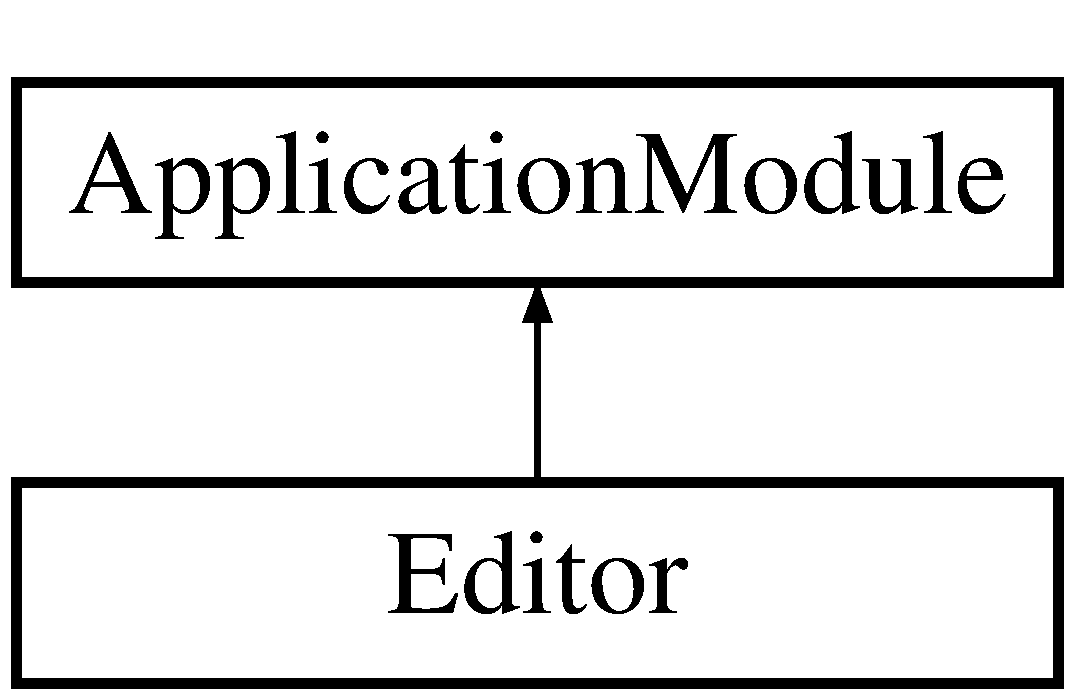
\includegraphics[height=2cm]{classEditor}
\end{center}
\end{figure}
\subsection*{Public Member Functions}
\begin{DoxyCompactItemize}
\item 
\hypertarget{classEditor_aa27188c2a247b99fb7a5a00229be9a6b}{
{\bfseries Editor} (CL\_\-DisplayWindow \&)}
\label{classEditor_aa27188c2a247b99fb7a5a00229be9a6b}

\end{DoxyCompactItemize}


\subsection{Detailed Description}
The editor class is used to edit the plot Baysian Networks. 

The documentation for this class was generated from the following files:\begin{DoxyCompactItemize}
\item 
source/editor/\hyperlink{Editor_8h}{Editor.h}\item 
source/editor/\hyperlink{Editor_8cpp}{Editor.cpp}\end{DoxyCompactItemize}

\hypertarget{structboost_1_1enable__if}{
\section{boost::enable\_\-if$<$ Cond, T $>$ Struct Template Reference}
\label{structboost_1_1enable__if}\index{boost::enable\_\-if@{boost::enable\_\-if}}
}
Inheritance diagram for boost::enable\_\-if$<$ Cond, T $>$::\begin{figure}[H]
\begin{center}
\leavevmode
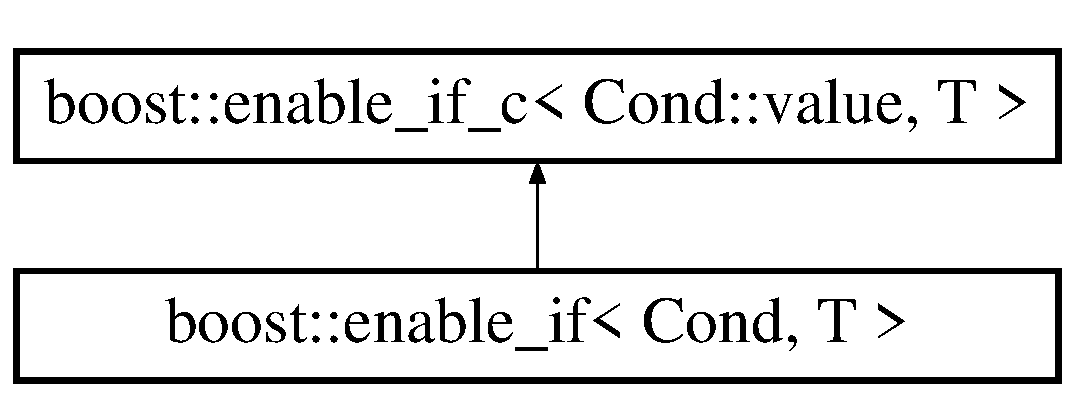
\includegraphics[height=2cm]{structboost_1_1enable__if}
\end{center}
\end{figure}
\subsubsection*{template$<$class Cond, class T = void$>$ struct boost::enable\_\-if$<$ Cond, T $>$}



The documentation for this struct was generated from the following file:\begin{DoxyCompactItemize}
\item 
source/dlib/enable\_\-if.h\end{DoxyCompactItemize}

\hypertarget{structboost_1_1enable__if__c}{
\section{boost::enable\_\-if\_\-c$<$ B, T $>$ Struct Template Reference}
\label{structboost_1_1enable__if__c}\index{boost::enable\_\-if\_\-c@{boost::enable\_\-if\_\-c}}
}
\subsection*{Public Types}
\begin{DoxyCompactItemize}
\item 
\hypertarget{structboost_1_1enable__if__c_ad0c840d6d2f1cccff0f54ec4e577cd84}{
typedef T {\bfseries type}}
\label{structboost_1_1enable__if__c_ad0c840d6d2f1cccff0f54ec4e577cd84}

\end{DoxyCompactItemize}
\subsubsection*{template$<$bool B, class T = void$>$ struct boost::enable\_\-if\_\-c$<$ B, T $>$}



The documentation for this struct was generated from the following file:\begin{DoxyCompactItemize}
\item 
source/dlib/enable\_\-if.h\end{DoxyCompactItemize}

\hypertarget{structboost_1_1enable__if__c_3_01false_00_01T_01_4}{
\section{boost::enable\_\-if\_\-c$<$ false, T $>$ Struct Template Reference}
\label{structboost_1_1enable__if__c_3_01false_00_01T_01_4}\index{boost::enable\_\-if\_\-c$<$ false, T $>$@{boost::enable\_\-if\_\-c$<$ false, T $>$}}
}
\subsubsection*{template$<$class T$>$ struct boost::enable\_\-if\_\-c$<$ false, T $>$}



The documentation for this struct was generated from the following file:\begin{DoxyCompactItemize}
\item 
source/dlib/enable\_\-if.h\end{DoxyCompactItemize}

\hypertarget{classdlib_1_1entropy__decoder}{
\section{dlib::entropy\_\-decoder Class Reference}
\label{classdlib_1_1entropy__decoder}\index{dlib::entropy\_\-decoder@{dlib::entropy\_\-decoder}}
}
\subsection*{Public Types}
\begin{DoxyCompactItemize}
\item 
\hypertarget{classdlib_1_1entropy__decoder_af02ac6bd1c208f37403e9efbcffd084a}{
typedef entropy\_\-decoder\_\-kernel\_\-1 {\bfseries kernel\_\-1a}}
\label{classdlib_1_1entropy__decoder_af02ac6bd1c208f37403e9efbcffd084a}

\item 
\hypertarget{classdlib_1_1entropy__decoder_af4473baff1a4e5f5a9d7630ee56118ed}{
typedef entropy\_\-decoder\_\-kernel\_\-c$<$ kernel\_\-1a $>$ {\bfseries kernel\_\-1a\_\-c}}
\label{classdlib_1_1entropy__decoder_af4473baff1a4e5f5a9d7630ee56118ed}

\item 
\hypertarget{classdlib_1_1entropy__decoder_a96ef43e2f5babdb5760c58261b54890a}{
typedef entropy\_\-decoder\_\-kernel\_\-2 {\bfseries kernel\_\-2a}}
\label{classdlib_1_1entropy__decoder_a96ef43e2f5babdb5760c58261b54890a}

\item 
\hypertarget{classdlib_1_1entropy__decoder_a3ed13be5412f1b6a6f60f00d24b42bd2}{
typedef entropy\_\-decoder\_\-kernel\_\-c$<$ kernel\_\-2a $>$ {\bfseries kernel\_\-2a\_\-c}}
\label{classdlib_1_1entropy__decoder_a3ed13be5412f1b6a6f60f00d24b42bd2}

\end{DoxyCompactItemize}


The documentation for this class was generated from the following file:\begin{DoxyCompactItemize}
\item 
source/dlib/entropy\_\-decoder.h\end{DoxyCompactItemize}

\hypertarget{classdlib_1_1entropy__decoder__model}{
\section{dlib::entropy\_\-decoder\_\-model$<$ alphabet\_\-size, entropy\_\-decoder $>$ Class Template Reference}
\label{classdlib_1_1entropy__decoder__model}\index{dlib::entropy\_\-decoder\_\-model@{dlib::entropy\_\-decoder\_\-model}}
}
\subsection*{Public Types}
\begin{DoxyCompactItemize}
\item 
\hypertarget{classdlib_1_1entropy__decoder__model_a1671912b73a04a01e27fd582c8e4d6b1}{
typedef entropy\_\-decoder\_\-model\_\-kernel\_\-1$<$ alphabet\_\-size, \hyperlink{classdlib_1_1entropy__decoder}{entropy\_\-decoder}, cc1 $>$ {\bfseries kernel\_\-1a}}
\label{classdlib_1_1entropy__decoder__model_a1671912b73a04a01e27fd582c8e4d6b1}

\item 
\hypertarget{classdlib_1_1entropy__decoder__model_a8e365a04a3dd0dafbda75f22577c1ef3}{
typedef entropy\_\-decoder\_\-model\_\-kernel\_\-1$<$ alphabet\_\-size, \hyperlink{classdlib_1_1entropy__decoder}{entropy\_\-decoder}, cc2 $>$ {\bfseries kernel\_\-1b}}
\label{classdlib_1_1entropy__decoder__model_a8e365a04a3dd0dafbda75f22577c1ef3}

\item 
\hypertarget{classdlib_1_1entropy__decoder__model_a9160a0902abe5f6d3c8c9ae06c0959fd}{
typedef entropy\_\-decoder\_\-model\_\-kernel\_\-1$<$ alphabet\_\-size, \hyperlink{classdlib_1_1entropy__decoder}{entropy\_\-decoder}, cc3 $>$ {\bfseries kernel\_\-1c}}
\label{classdlib_1_1entropy__decoder__model_a9160a0902abe5f6d3c8c9ae06c0959fd}

\item 
\hypertarget{classdlib_1_1entropy__decoder__model_a227d0988724460290cbdd84935b23f7e}{
typedef entropy\_\-decoder\_\-model\_\-kernel\_\-2$<$ alphabet\_\-size, \hyperlink{classdlib_1_1entropy__decoder}{entropy\_\-decoder}, cc1, cc1 $>$ {\bfseries kernel\_\-2a}}
\label{classdlib_1_1entropy__decoder__model_a227d0988724460290cbdd84935b23f7e}

\item 
\hypertarget{classdlib_1_1entropy__decoder__model_aa1dc8470ffa66eb9d27859d300d35082}{
typedef entropy\_\-decoder\_\-model\_\-kernel\_\-2$<$ alphabet\_\-size, \hyperlink{classdlib_1_1entropy__decoder}{entropy\_\-decoder}, cc2, cc2 $>$ {\bfseries kernel\_\-2b}}
\label{classdlib_1_1entropy__decoder__model_aa1dc8470ffa66eb9d27859d300d35082}

\item 
\hypertarget{classdlib_1_1entropy__decoder__model_a780b5fd2fd269af6308e69dbab9a6c43}{
typedef entropy\_\-decoder\_\-model\_\-kernel\_\-2$<$ alphabet\_\-size, \hyperlink{classdlib_1_1entropy__decoder}{entropy\_\-decoder}, cc3, cc3 $>$ {\bfseries kernel\_\-2c}}
\label{classdlib_1_1entropy__decoder__model_a780b5fd2fd269af6308e69dbab9a6c43}

\item 
\hypertarget{classdlib_1_1entropy__decoder__model_a96c64b6c563ba5520680ceb31af1d1a7}{
typedef entropy\_\-decoder\_\-model\_\-kernel\_\-2$<$ alphabet\_\-size, \hyperlink{classdlib_1_1entropy__decoder}{entropy\_\-decoder}, cc2, cc4b $>$ {\bfseries kernel\_\-2d}}
\label{classdlib_1_1entropy__decoder__model_a96c64b6c563ba5520680ceb31af1d1a7}

\item 
\hypertarget{classdlib_1_1entropy__decoder__model_afeb314a8bf069c2a8fb0518b1e00a635}{
typedef entropy\_\-decoder\_\-model\_\-kernel\_\-3$<$ alphabet\_\-size, \hyperlink{classdlib_1_1entropy__decoder}{entropy\_\-decoder}, cc1, cc4b $>$ {\bfseries kernel\_\-3a}}
\label{classdlib_1_1entropy__decoder__model_afeb314a8bf069c2a8fb0518b1e00a635}

\item 
\hypertarget{classdlib_1_1entropy__decoder__model_a3f9cb0b1f6fc5ee461c6afabb9687635}{
typedef entropy\_\-decoder\_\-model\_\-kernel\_\-3$<$ alphabet\_\-size, \hyperlink{classdlib_1_1entropy__decoder}{entropy\_\-decoder}, cc2, cc4b $>$ {\bfseries kernel\_\-3b}}
\label{classdlib_1_1entropy__decoder__model_a3f9cb0b1f6fc5ee461c6afabb9687635}

\item 
\hypertarget{classdlib_1_1entropy__decoder__model_aa370da51f4d116b84925e26614edbcce}{
typedef entropy\_\-decoder\_\-model\_\-kernel\_\-3$<$ alphabet\_\-size, \hyperlink{classdlib_1_1entropy__decoder}{entropy\_\-decoder}, cc3, cc4b $>$ {\bfseries kernel\_\-3c}}
\label{classdlib_1_1entropy__decoder__model_aa370da51f4d116b84925e26614edbcce}

\item 
\hypertarget{classdlib_1_1entropy__decoder__model_af88608a41e688b008ef899c8b58824fc}{
typedef entropy\_\-decoder\_\-model\_\-kernel\_\-4$<$ alphabet\_\-size, \hyperlink{classdlib_1_1entropy__decoder}{entropy\_\-decoder}, 200000, 4 $>$ {\bfseries kernel\_\-4a}}
\label{classdlib_1_1entropy__decoder__model_af88608a41e688b008ef899c8b58824fc}

\item 
\hypertarget{classdlib_1_1entropy__decoder__model_accc6eaa778f23bfc9973cdfc20196c13}{
typedef entropy\_\-decoder\_\-model\_\-kernel\_\-4$<$ alphabet\_\-size, \hyperlink{classdlib_1_1entropy__decoder}{entropy\_\-decoder}, 1000000, 5 $>$ {\bfseries kernel\_\-4b}}
\label{classdlib_1_1entropy__decoder__model_accc6eaa778f23bfc9973cdfc20196c13}

\item 
\hypertarget{classdlib_1_1entropy__decoder__model_a9ec3613cee5a64993dbf44e9d32bbbdc}{
typedef entropy\_\-decoder\_\-model\_\-kernel\_\-5$<$ alphabet\_\-size, \hyperlink{classdlib_1_1entropy__decoder}{entropy\_\-decoder}, 200000, 4 $>$ {\bfseries kernel\_\-5a}}
\label{classdlib_1_1entropy__decoder__model_a9ec3613cee5a64993dbf44e9d32bbbdc}

\item 
\hypertarget{classdlib_1_1entropy__decoder__model_a85aedf944576b934da4652be16486bcc}{
typedef entropy\_\-decoder\_\-model\_\-kernel\_\-5$<$ alphabet\_\-size, \hyperlink{classdlib_1_1entropy__decoder}{entropy\_\-decoder}, 1000000, 5 $>$ {\bfseries kernel\_\-5b}}
\label{classdlib_1_1entropy__decoder__model_a85aedf944576b934da4652be16486bcc}

\item 
\hypertarget{classdlib_1_1entropy__decoder__model_a1a0a7e4b6eebe178222f8846af5d3b2b}{
typedef entropy\_\-decoder\_\-model\_\-kernel\_\-5$<$ alphabet\_\-size, \hyperlink{classdlib_1_1entropy__decoder}{entropy\_\-decoder}, 2500000, 7 $>$ {\bfseries kernel\_\-5c}}
\label{classdlib_1_1entropy__decoder__model_a1a0a7e4b6eebe178222f8846af5d3b2b}

\item 
\hypertarget{classdlib_1_1entropy__decoder__model_a898904b2221a1bde850ae3429390c279}{
typedef entropy\_\-decoder\_\-model\_\-kernel\_\-6$<$ alphabet\_\-size, \hyperlink{classdlib_1_1entropy__decoder}{entropy\_\-decoder} $>$ {\bfseries kernel\_\-6a}}
\label{classdlib_1_1entropy__decoder__model_a898904b2221a1bde850ae3429390c279}

\end{DoxyCompactItemize}
\subsubsection*{template$<$unsigned long alphabet\_\-size, typename entropy\_\-decoder$>$ class dlib::entropy\_\-decoder\_\-model$<$ alphabet\_\-size, entropy\_\-decoder $>$}



The documentation for this class was generated from the following file:\begin{DoxyCompactItemize}
\item 
source/dlib/entropy\_\-decoder\_\-model.h\end{DoxyCompactItemize}

\hypertarget{classdlib_1_1entropy__encoder}{
\section{dlib::entropy\_\-encoder Class Reference}
\label{classdlib_1_1entropy__encoder}\index{dlib::entropy\_\-encoder@{dlib::entropy\_\-encoder}}
}
\subsection*{Public Types}
\begin{DoxyCompactItemize}
\item 
\hypertarget{classdlib_1_1entropy__encoder_a6a75b09b663d75271eb52b3251a61184}{
typedef entropy\_\-encoder\_\-kernel\_\-1 {\bfseries kernel\_\-1a}}
\label{classdlib_1_1entropy__encoder_a6a75b09b663d75271eb52b3251a61184}

\item 
\hypertarget{classdlib_1_1entropy__encoder_a3ddb2f06e846e0c096e61a768bda1ec5}{
typedef entropy\_\-encoder\_\-kernel\_\-c$<$ kernel\_\-1a $>$ {\bfseries kernel\_\-1a\_\-c}}
\label{classdlib_1_1entropy__encoder_a3ddb2f06e846e0c096e61a768bda1ec5}

\item 
\hypertarget{classdlib_1_1entropy__encoder_a38fe35a19eda6e5b05482a43911ede17}{
typedef entropy\_\-encoder\_\-kernel\_\-2 {\bfseries kernel\_\-2a}}
\label{classdlib_1_1entropy__encoder_a38fe35a19eda6e5b05482a43911ede17}

\item 
\hypertarget{classdlib_1_1entropy__encoder_a92b57876edb98c24d52412ee97b208a2}{
typedef entropy\_\-encoder\_\-kernel\_\-c$<$ kernel\_\-2a $>$ {\bfseries kernel\_\-2a\_\-c}}
\label{classdlib_1_1entropy__encoder_a92b57876edb98c24d52412ee97b208a2}

\end{DoxyCompactItemize}


The documentation for this class was generated from the following file:\begin{DoxyCompactItemize}
\item 
source/dlib/entropy\_\-encoder.h\end{DoxyCompactItemize}

\hypertarget{classdlib_1_1entropy__encoder__model}{
\section{dlib::entropy\_\-encoder\_\-model$<$ alphabet\_\-size, entropy\_\-encoder $>$ Class Template Reference}
\label{classdlib_1_1entropy__encoder__model}\index{dlib::entropy\_\-encoder\_\-model@{dlib::entropy\_\-encoder\_\-model}}
}
\subsection*{Public Types}
\begin{DoxyCompactItemize}
\item 
\hypertarget{classdlib_1_1entropy__encoder__model_a127ce2530aac8ba46899b29aaf8bad86}{
typedef entropy\_\-encoder\_\-model\_\-kernel\_\-1$<$ alphabet\_\-size, \hyperlink{classdlib_1_1entropy__encoder}{entropy\_\-encoder}, cc1 $>$ {\bfseries kernel\_\-1a}}
\label{classdlib_1_1entropy__encoder__model_a127ce2530aac8ba46899b29aaf8bad86}

\item 
\hypertarget{classdlib_1_1entropy__encoder__model_aec9d6e5bdcac8a7853eb2a7fabe54598}{
typedef entropy\_\-encoder\_\-model\_\-kernel\_\-c$<$ kernel\_\-1a $>$ {\bfseries kernel\_\-1a\_\-c}}
\label{classdlib_1_1entropy__encoder__model_aec9d6e5bdcac8a7853eb2a7fabe54598}

\item 
\hypertarget{classdlib_1_1entropy__encoder__model_a2ad3f3936f18afac3236e7258fa37251}{
typedef entropy\_\-encoder\_\-model\_\-kernel\_\-1$<$ alphabet\_\-size, \hyperlink{classdlib_1_1entropy__encoder}{entropy\_\-encoder}, cc2 $>$ {\bfseries kernel\_\-1b}}
\label{classdlib_1_1entropy__encoder__model_a2ad3f3936f18afac3236e7258fa37251}

\item 
\hypertarget{classdlib_1_1entropy__encoder__model_ac89ba7f46967adb8b5a942b298d05bea}{
typedef entropy\_\-encoder\_\-model\_\-kernel\_\-c$<$ kernel\_\-1b $>$ {\bfseries kernel\_\-1b\_\-c}}
\label{classdlib_1_1entropy__encoder__model_ac89ba7f46967adb8b5a942b298d05bea}

\item 
\hypertarget{classdlib_1_1entropy__encoder__model_a75a1dd89362256f5da51dceb35460bdc}{
typedef entropy\_\-encoder\_\-model\_\-kernel\_\-1$<$ alphabet\_\-size, \hyperlink{classdlib_1_1entropy__encoder}{entropy\_\-encoder}, cc3 $>$ {\bfseries kernel\_\-1c}}
\label{classdlib_1_1entropy__encoder__model_a75a1dd89362256f5da51dceb35460bdc}

\item 
\hypertarget{classdlib_1_1entropy__encoder__model_a29abf00894e8882bfb874b8f3afad42d}{
typedef entropy\_\-encoder\_\-model\_\-kernel\_\-c$<$ kernel\_\-1c $>$ {\bfseries kernel\_\-1c\_\-c}}
\label{classdlib_1_1entropy__encoder__model_a29abf00894e8882bfb874b8f3afad42d}

\item 
\hypertarget{classdlib_1_1entropy__encoder__model_a5fda4508a3ecd0a38b45093d77ad3808}{
typedef entropy\_\-encoder\_\-model\_\-kernel\_\-2$<$ alphabet\_\-size, \hyperlink{classdlib_1_1entropy__encoder}{entropy\_\-encoder}, cc1, cc1 $>$ {\bfseries kernel\_\-2a}}
\label{classdlib_1_1entropy__encoder__model_a5fda4508a3ecd0a38b45093d77ad3808}

\item 
\hypertarget{classdlib_1_1entropy__encoder__model_a6c76cfb361686eeae870da83d1330ecf}{
typedef entropy\_\-encoder\_\-model\_\-kernel\_\-c$<$ kernel\_\-2a $>$ {\bfseries kernel\_\-2a\_\-c}}
\label{classdlib_1_1entropy__encoder__model_a6c76cfb361686eeae870da83d1330ecf}

\item 
\hypertarget{classdlib_1_1entropy__encoder__model_a2feb7caabe8e2c3519829b9f12be222a}{
typedef entropy\_\-encoder\_\-model\_\-kernel\_\-2$<$ alphabet\_\-size, \hyperlink{classdlib_1_1entropy__encoder}{entropy\_\-encoder}, cc2, cc2 $>$ {\bfseries kernel\_\-2b}}
\label{classdlib_1_1entropy__encoder__model_a2feb7caabe8e2c3519829b9f12be222a}

\item 
\hypertarget{classdlib_1_1entropy__encoder__model_ad78ee85da043cb0fdf9242fe60dcbe01}{
typedef entropy\_\-encoder\_\-model\_\-kernel\_\-c$<$ kernel\_\-2b $>$ {\bfseries kernel\_\-2b\_\-c}}
\label{classdlib_1_1entropy__encoder__model_ad78ee85da043cb0fdf9242fe60dcbe01}

\item 
\hypertarget{classdlib_1_1entropy__encoder__model_ab1a973c444a47a3d2a97296b9f9b5fb2}{
typedef entropy\_\-encoder\_\-model\_\-kernel\_\-2$<$ alphabet\_\-size, \hyperlink{classdlib_1_1entropy__encoder}{entropy\_\-encoder}, cc3, cc3 $>$ {\bfseries kernel\_\-2c}}
\label{classdlib_1_1entropy__encoder__model_ab1a973c444a47a3d2a97296b9f9b5fb2}

\item 
\hypertarget{classdlib_1_1entropy__encoder__model_acc50842f3c7f55e7305a5f359b2a9966}{
typedef entropy\_\-encoder\_\-model\_\-kernel\_\-c$<$ kernel\_\-2c $>$ {\bfseries kernel\_\-2c\_\-c}}
\label{classdlib_1_1entropy__encoder__model_acc50842f3c7f55e7305a5f359b2a9966}

\item 
\hypertarget{classdlib_1_1entropy__encoder__model_a5e03f6d4a8b52e3e2667134bb821d224}{
typedef entropy\_\-encoder\_\-model\_\-kernel\_\-2$<$ alphabet\_\-size, \hyperlink{classdlib_1_1entropy__encoder}{entropy\_\-encoder}, cc2, cc4b $>$ {\bfseries kernel\_\-2d}}
\label{classdlib_1_1entropy__encoder__model_a5e03f6d4a8b52e3e2667134bb821d224}

\item 
\hypertarget{classdlib_1_1entropy__encoder__model_a065fb640734929aa764a22a2159d0053}{
typedef entropy\_\-encoder\_\-model\_\-kernel\_\-c$<$ kernel\_\-2d $>$ {\bfseries kernel\_\-2d\_\-c}}
\label{classdlib_1_1entropy__encoder__model_a065fb640734929aa764a22a2159d0053}

\item 
\hypertarget{classdlib_1_1entropy__encoder__model_afe9d7573593b4a4218ab7daeea1c9181}{
typedef entropy\_\-encoder\_\-model\_\-kernel\_\-3$<$ alphabet\_\-size, \hyperlink{classdlib_1_1entropy__encoder}{entropy\_\-encoder}, cc1, cc4b $>$ {\bfseries kernel\_\-3a}}
\label{classdlib_1_1entropy__encoder__model_afe9d7573593b4a4218ab7daeea1c9181}

\item 
\hypertarget{classdlib_1_1entropy__encoder__model_aeaac6bdadbf9e6cf430b2a46ab72d26c}{
typedef entropy\_\-encoder\_\-model\_\-kernel\_\-c$<$ kernel\_\-3a $>$ {\bfseries kernel\_\-3a\_\-c}}
\label{classdlib_1_1entropy__encoder__model_aeaac6bdadbf9e6cf430b2a46ab72d26c}

\item 
\hypertarget{classdlib_1_1entropy__encoder__model_a40b97b86224a48ce04524dedcbe8afd9}{
typedef entropy\_\-encoder\_\-model\_\-kernel\_\-3$<$ alphabet\_\-size, \hyperlink{classdlib_1_1entropy__encoder}{entropy\_\-encoder}, cc2, cc4b $>$ {\bfseries kernel\_\-3b}}
\label{classdlib_1_1entropy__encoder__model_a40b97b86224a48ce04524dedcbe8afd9}

\item 
\hypertarget{classdlib_1_1entropy__encoder__model_aa8bae2d5965ed9a80b39711e42ac5c07}{
typedef entropy\_\-encoder\_\-model\_\-kernel\_\-c$<$ kernel\_\-3b $>$ {\bfseries kernel\_\-3b\_\-c}}
\label{classdlib_1_1entropy__encoder__model_aa8bae2d5965ed9a80b39711e42ac5c07}

\item 
\hypertarget{classdlib_1_1entropy__encoder__model_ad97b6017ca7cca419f29216e8afb4cad}{
typedef entropy\_\-encoder\_\-model\_\-kernel\_\-3$<$ alphabet\_\-size, \hyperlink{classdlib_1_1entropy__encoder}{entropy\_\-encoder}, cc3, cc4b $>$ {\bfseries kernel\_\-3c}}
\label{classdlib_1_1entropy__encoder__model_ad97b6017ca7cca419f29216e8afb4cad}

\item 
\hypertarget{classdlib_1_1entropy__encoder__model_ada5dda665042404177eef75ba9e169b4}{
typedef entropy\_\-encoder\_\-model\_\-kernel\_\-c$<$ kernel\_\-3c $>$ {\bfseries kernel\_\-3c\_\-c}}
\label{classdlib_1_1entropy__encoder__model_ada5dda665042404177eef75ba9e169b4}

\item 
\hypertarget{classdlib_1_1entropy__encoder__model_a29218a56d9d475c535a1b1e8982905c8}{
typedef entropy\_\-encoder\_\-model\_\-kernel\_\-4$<$ alphabet\_\-size, \hyperlink{classdlib_1_1entropy__encoder}{entropy\_\-encoder}, 200000, 4 $>$ {\bfseries kernel\_\-4a}}
\label{classdlib_1_1entropy__encoder__model_a29218a56d9d475c535a1b1e8982905c8}

\item 
\hypertarget{classdlib_1_1entropy__encoder__model_a7861183dc9f9f9594f2c174208d1d5b2}{
typedef entropy\_\-encoder\_\-model\_\-kernel\_\-c$<$ kernel\_\-4a $>$ {\bfseries kernel\_\-4a\_\-c}}
\label{classdlib_1_1entropy__encoder__model_a7861183dc9f9f9594f2c174208d1d5b2}

\item 
\hypertarget{classdlib_1_1entropy__encoder__model_a1ab43f7622e44a36a541eda4308f5c9c}{
typedef entropy\_\-encoder\_\-model\_\-kernel\_\-4$<$ alphabet\_\-size, \hyperlink{classdlib_1_1entropy__encoder}{entropy\_\-encoder}, 1000000, 5 $>$ {\bfseries kernel\_\-4b}}
\label{classdlib_1_1entropy__encoder__model_a1ab43f7622e44a36a541eda4308f5c9c}

\item 
\hypertarget{classdlib_1_1entropy__encoder__model_a35672d32222e8caecf0338736c994007}{
typedef entropy\_\-encoder\_\-model\_\-kernel\_\-c$<$ kernel\_\-4b $>$ {\bfseries kernel\_\-4b\_\-c}}
\label{classdlib_1_1entropy__encoder__model_a35672d32222e8caecf0338736c994007}

\item 
\hypertarget{classdlib_1_1entropy__encoder__model_a22266733246a977476944361625f03af}{
typedef entropy\_\-encoder\_\-model\_\-kernel\_\-5$<$ alphabet\_\-size, \hyperlink{classdlib_1_1entropy__encoder}{entropy\_\-encoder}, 200000, 4 $>$ {\bfseries kernel\_\-5a}}
\label{classdlib_1_1entropy__encoder__model_a22266733246a977476944361625f03af}

\item 
\hypertarget{classdlib_1_1entropy__encoder__model_a5c270e4e7dd1cb431e7d8cd673bf47ec}{
typedef entropy\_\-encoder\_\-model\_\-kernel\_\-c$<$ kernel\_\-5a $>$ {\bfseries kernel\_\-5a\_\-c}}
\label{classdlib_1_1entropy__encoder__model_a5c270e4e7dd1cb431e7d8cd673bf47ec}

\item 
\hypertarget{classdlib_1_1entropy__encoder__model_a7299539ddefa6e9936bdbcf9205dcc55}{
typedef entropy\_\-encoder\_\-model\_\-kernel\_\-5$<$ alphabet\_\-size, \hyperlink{classdlib_1_1entropy__encoder}{entropy\_\-encoder}, 1000000, 5 $>$ {\bfseries kernel\_\-5b}}
\label{classdlib_1_1entropy__encoder__model_a7299539ddefa6e9936bdbcf9205dcc55}

\item 
\hypertarget{classdlib_1_1entropy__encoder__model_a491aeb366f9db424635a462772cb40b0}{
typedef entropy\_\-encoder\_\-model\_\-kernel\_\-c$<$ kernel\_\-5b $>$ {\bfseries kernel\_\-5b\_\-c}}
\label{classdlib_1_1entropy__encoder__model_a491aeb366f9db424635a462772cb40b0}

\item 
\hypertarget{classdlib_1_1entropy__encoder__model_a0f5b9599644ce21dca4c78593f44282d}{
typedef entropy\_\-encoder\_\-model\_\-kernel\_\-5$<$ alphabet\_\-size, \hyperlink{classdlib_1_1entropy__encoder}{entropy\_\-encoder}, 2500000, 7 $>$ {\bfseries kernel\_\-5c}}
\label{classdlib_1_1entropy__encoder__model_a0f5b9599644ce21dca4c78593f44282d}

\item 
\hypertarget{classdlib_1_1entropy__encoder__model_a4cc527c8f4684281e866a06409028ac4}{
typedef entropy\_\-encoder\_\-model\_\-kernel\_\-c$<$ kernel\_\-5c $>$ {\bfseries kernel\_\-5c\_\-c}}
\label{classdlib_1_1entropy__encoder__model_a4cc527c8f4684281e866a06409028ac4}

\item 
\hypertarget{classdlib_1_1entropy__encoder__model_a7086dd46c383a76ba2ae9c88bd25a646}{
typedef entropy\_\-encoder\_\-model\_\-kernel\_\-6$<$ alphabet\_\-size, \hyperlink{classdlib_1_1entropy__encoder}{entropy\_\-encoder} $>$ {\bfseries kernel\_\-6a}}
\label{classdlib_1_1entropy__encoder__model_a7086dd46c383a76ba2ae9c88bd25a646}

\item 
\hypertarget{classdlib_1_1entropy__encoder__model_a608120f100790cfbbe4681bcd15e9cd4}{
typedef entropy\_\-encoder\_\-model\_\-kernel\_\-c$<$ kernel\_\-6a $>$ {\bfseries kernel\_\-6a\_\-c}}
\label{classdlib_1_1entropy__encoder__model_a608120f100790cfbbe4681bcd15e9cd4}

\end{DoxyCompactItemize}
\subsubsection*{template$<$unsigned long alphabet\_\-size, typename entropy\_\-encoder$>$ class dlib::entropy\_\-encoder\_\-model$<$ alphabet\_\-size, entropy\_\-encoder $>$}



The documentation for this class was generated from the following file:\begin{DoxyCompactItemize}
\item 
source/dlib/entropy\_\-encoder\_\-model.h\end{DoxyCompactItemize}

\hypertarget{classdlib_1_1error}{
\section{dlib::error Class Reference}
\label{classdlib_1_1error}\index{dlib::error@{dlib::error}}
}
Inheritance diagram for dlib::error::\begin{figure}[H]
\begin{center}
\leavevmode
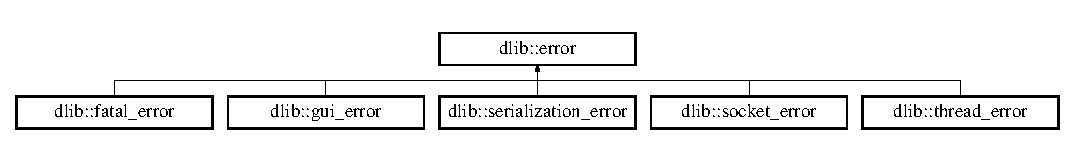
\includegraphics[height=1.50336cm]{classdlib_1_1error}
\end{center}
\end{figure}
\subsection*{Public Member Functions}
\begin{DoxyCompactItemize}
\item 
\hyperlink{classdlib_1_1error_a9bf6adbf16ad50c6a509b4e18d6becaa}{error} (error\_\-type t, const std::string \&a)
\item 
\hyperlink{classdlib_1_1error_aef92e7c614783f7a1290b8430dc3bea8}{error} (error\_\-type t)
\item 
\hyperlink{classdlib_1_1error_a05e6b9e17d00751f4603b9b19774fcc0}{error} (const std::string \&a)
\item 
\hyperlink{classdlib_1_1error_a7aa811457dae46c97d8b9ecc696b0559}{error} ()
\item 
virtual \hyperlink{classdlib_1_1error_ab9a83be4747253f0450091206efa901f}{$\sim$error} ()  throw ()
\item 
const char $\ast$ \hyperlink{classdlib_1_1error_a5f469c24dbcb32b0f83f66ded3609e92}{what} () const   throw ()
\item 
const char $\ast$ \hyperlink{classdlib_1_1error_aa45c616e14dd55887ad8b6f8b7b2e9aa}{type\_\-to\_\-string} () const   throw ()
\end{DoxyCompactItemize}
\subsection*{Public Attributes}
\begin{DoxyCompactItemize}
\item 
\hypertarget{classdlib_1_1error_a1c79d2462200ab506098b4c921ee6776}{
const std::string {\bfseries info}}
\label{classdlib_1_1error_a1c79d2462200ab506098b4c921ee6776}

\item 
\hypertarget{classdlib_1_1error_ab7e9eb19d8033a682d096a31192de73f}{
const error\_\-type {\bfseries type}}
\label{classdlib_1_1error_ab7e9eb19d8033a682d096a31192de73f}

\end{DoxyCompactItemize}


\subsection{Constructor \& Destructor Documentation}
\hypertarget{classdlib_1_1error_a9bf6adbf16ad50c6a509b4e18d6becaa}{
\index{dlib::error@{dlib::error}!error@{error}}
\index{error@{error}!dlib::error@{dlib::error}}
\subsubsection[{error}]{\setlength{\rightskip}{0pt plus 5cm}dlib::error::error (error\_\-type {\em t}, \/  const std::string \& {\em a})\hspace{0.3cm}{\ttfamily  \mbox{[}inline\mbox{]}}}}
\label{classdlib_1_1error_a9bf6adbf16ad50c6a509b4e18d6becaa}
WHAT THIS OBJECT REPRESENTS This is the base exception class for the \hyperlink{namespacedlib}{dlib} library. i.e. all exceptions in this library inherit from this class. ! \hypertarget{classdlib_1_1error_aef92e7c614783f7a1290b8430dc3bea8}{
\index{dlib::error@{dlib::error}!error@{error}}
\index{error@{error}!dlib::error@{dlib::error}}
\subsubsection[{error}]{\setlength{\rightskip}{0pt plus 5cm}dlib::error::error (error\_\-type {\em t})\hspace{0.3cm}{\ttfamily  \mbox{[}inline\mbox{]}}}}
\label{classdlib_1_1error_aef92e7c614783f7a1290b8430dc3bea8}
ensures
\begin{DoxyItemize}
\item type == t
\item info == a ! 
\end{DoxyItemize}\hypertarget{classdlib_1_1error_a05e6b9e17d00751f4603b9b19774fcc0}{
\index{dlib::error@{dlib::error}!error@{error}}
\index{error@{error}!dlib::error@{dlib::error}}
\subsubsection[{error}]{\setlength{\rightskip}{0pt plus 5cm}dlib::error::error (const std::string \& {\em a})\hspace{0.3cm}{\ttfamily  \mbox{[}inline\mbox{]}}}}
\label{classdlib_1_1error_a05e6b9e17d00751f4603b9b19774fcc0}
ensures
\begin{DoxyItemize}
\item type == t
\item info == \char`\"{}\char`\"{} ! 
\end{DoxyItemize}\hypertarget{classdlib_1_1error_a7aa811457dae46c97d8b9ecc696b0559}{
\index{dlib::error@{dlib::error}!error@{error}}
\index{error@{error}!dlib::error@{dlib::error}}
\subsubsection[{error}]{\setlength{\rightskip}{0pt plus 5cm}dlib::error::error ()\hspace{0.3cm}{\ttfamily  \mbox{[}inline\mbox{]}}}}
\label{classdlib_1_1error_a7aa811457dae46c97d8b9ecc696b0559}
ensures
\begin{DoxyItemize}
\item type == EUNSPECIFIED
\item info == a ! 
\end{DoxyItemize}\hypertarget{classdlib_1_1error_ab9a83be4747253f0450091206efa901f}{
\index{dlib::error@{dlib::error}!$\sim$error@{$\sim$error}}
\index{$\sim$error@{$\sim$error}!dlib::error@{dlib::error}}
\subsubsection[{$\sim$error}]{\setlength{\rightskip}{0pt plus 5cm}virtual dlib::error::$\sim$error ()  throw ()\hspace{0.3cm}{\ttfamily  \mbox{[}inline, virtual\mbox{]}}}}
\label{classdlib_1_1error_ab9a83be4747253f0450091206efa901f}
ensures
\begin{DoxyItemize}
\item type == EUNSPECIFIED
\item info == \char`\"{}\char`\"{} ! 
\end{DoxyItemize}

\subsection{Member Function Documentation}
\hypertarget{classdlib_1_1error_aa45c616e14dd55887ad8b6f8b7b2e9aa}{
\index{dlib::error@{dlib::error}!type\_\-to\_\-string@{type\_\-to\_\-string}}
\index{type\_\-to\_\-string@{type\_\-to\_\-string}!dlib::error@{dlib::error}}
\subsubsection[{type\_\-to\_\-string}]{\setlength{\rightskip}{0pt plus 5cm}const char$\ast$ dlib::error::type\_\-to\_\-string () const  throw ()\hspace{0.3cm}{\ttfamily  \mbox{[}inline\mbox{]}}}}
\label{classdlib_1_1error_aa45c616e14dd55887ad8b6f8b7b2e9aa}
ensures
\begin{DoxyItemize}
\item returns a string that names the contents of the type member. ! 
\end{DoxyItemize}\hypertarget{classdlib_1_1error_a5f469c24dbcb32b0f83f66ded3609e92}{
\index{dlib::error@{dlib::error}!what@{what}}
\index{what@{what}!dlib::error@{dlib::error}}
\subsubsection[{what}]{\setlength{\rightskip}{0pt plus 5cm}const char$\ast$ dlib::error::what () const  throw ()\hspace{0.3cm}{\ttfamily  \mbox{[}inline\mbox{]}}}}
\label{classdlib_1_1error_a5f469c24dbcb32b0f83f66ded3609e92}
ensures
\begin{DoxyItemize}
\item does nothing !
\end{DoxyItemize}

ensures
\begin{DoxyItemize}
\item if (info.size() != 0) then
\begin{DoxyItemize}
\item returns info.c\_\-str()
\end{DoxyItemize}
\item else
\begin{DoxyItemize}
\item returns type\_\-to\_\-string(type) ! 
\end{DoxyItemize}
\end{DoxyItemize}

The documentation for this class was generated from the following file:\begin{DoxyCompactItemize}
\item 
source/dlib/error.h\end{DoxyCompactItemize}

\hypertarget{classdlib_1_1fatal__error}{
\section{dlib::fatal\_\-error Class Reference}
\label{classdlib_1_1fatal__error}\index{dlib::fatal\_\-error@{dlib::fatal\_\-error}}
}
Inheritance diagram for dlib::fatal\_\-error::\begin{figure}[H]
\begin{center}
\leavevmode
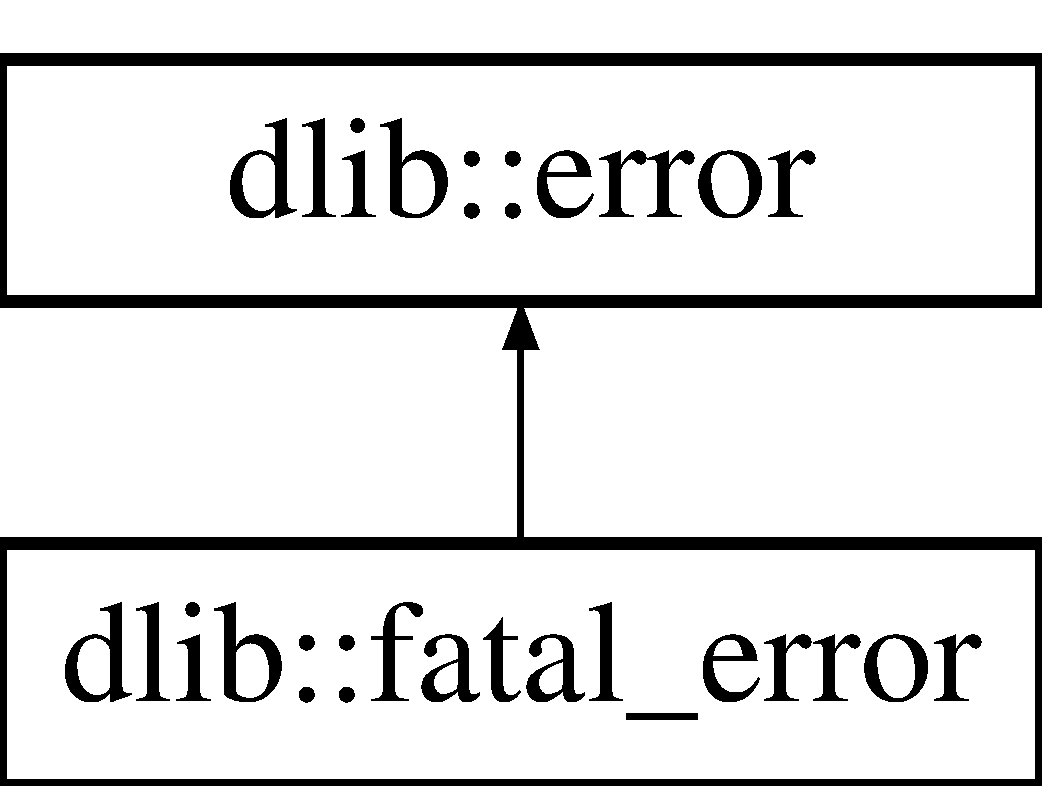
\includegraphics[height=2cm]{classdlib_1_1fatal__error}
\end{center}
\end{figure}
\subsection*{Public Member Functions}
\begin{DoxyCompactItemize}
\item 
\hyperlink{classdlib_1_1fatal__error_ae1ade5e6456e25e8b60ff532ed5e2e23}{fatal\_\-error} (error\_\-type t, const std::string \&a)
\item 
\hyperlink{classdlib_1_1fatal__error_ac947f78667e0aeba05ab738c3ab527d6}{fatal\_\-error} (error\_\-type t)
\item 
\hyperlink{classdlib_1_1fatal__error_a449542aaaf1cb427faa542bf369ca607}{fatal\_\-error} (const std::string \&a)
\item 
\hyperlink{classdlib_1_1fatal__error_ad824e88fda1a7e4e0fad7b147730dcfc}{fatal\_\-error} ()
\end{DoxyCompactItemize}


\subsection{Constructor \& Destructor Documentation}
\hypertarget{classdlib_1_1fatal__error_ae1ade5e6456e25e8b60ff532ed5e2e23}{
\index{dlib::fatal\_\-error@{dlib::fatal\_\-error}!fatal\_\-error@{fatal\_\-error}}
\index{fatal\_\-error@{fatal\_\-error}!dlib::fatal_error@{dlib::fatal\_\-error}}
\subsubsection[{fatal\_\-error}]{\setlength{\rightskip}{0pt plus 5cm}dlib::fatal\_\-error::fatal\_\-error (error\_\-type {\em t}, \/  const std::string \& {\em a})\hspace{0.3cm}{\ttfamily  \mbox{[}inline\mbox{]}}}}
\label{classdlib_1_1fatal__error_ae1ade5e6456e25e8b60ff532ed5e2e23}
WHAT THIS OBJECT REPRESENTS As the name says, this object represents some kind of fatal \hyperlink{classdlib_1_1error}{error}. That is, it represents an unrecoverable \hyperlink{classdlib_1_1error}{error} and any program that throws this exception is, by definition, buggy and needs to be fixed.

Note that a \hyperlink{classdlib_1_1fatal__error}{fatal\_\-error} exception can only be thrown once. The second time an application attempts to construct a \hyperlink{classdlib_1_1fatal__error}{fatal\_\-error} it will be immediately aborted and an \hyperlink{classdlib_1_1error}{error} message will be printed to std::cerr. The reason for this is because the first \hyperlink{classdlib_1_1fatal__error}{fatal\_\-error} was apparently ignored so the second \hyperlink{classdlib_1_1fatal__error}{fatal\_\-error} is going to make itself impossible to ignore by calling abort. The lesson here is that you should not try to ignore fatal errors.

This is also the exception thrown by the DLIB\_\-ASSERT and DLIB\_\-CASSERT macros. ! \hypertarget{classdlib_1_1fatal__error_ac947f78667e0aeba05ab738c3ab527d6}{
\index{dlib::fatal\_\-error@{dlib::fatal\_\-error}!fatal\_\-error@{fatal\_\-error}}
\index{fatal\_\-error@{fatal\_\-error}!dlib::fatal_error@{dlib::fatal\_\-error}}
\subsubsection[{fatal\_\-error}]{\setlength{\rightskip}{0pt plus 5cm}dlib::fatal\_\-error::fatal\_\-error (error\_\-type {\em t})\hspace{0.3cm}{\ttfamily  \mbox{[}inline\mbox{]}}}}
\label{classdlib_1_1fatal__error_ac947f78667e0aeba05ab738c3ab527d6}
ensures
\begin{DoxyItemize}
\item type == t
\item info == a ! 
\end{DoxyItemize}\hypertarget{classdlib_1_1fatal__error_a449542aaaf1cb427faa542bf369ca607}{
\index{dlib::fatal\_\-error@{dlib::fatal\_\-error}!fatal\_\-error@{fatal\_\-error}}
\index{fatal\_\-error@{fatal\_\-error}!dlib::fatal_error@{dlib::fatal\_\-error}}
\subsubsection[{fatal\_\-error}]{\setlength{\rightskip}{0pt plus 5cm}dlib::fatal\_\-error::fatal\_\-error (const std::string \& {\em a})\hspace{0.3cm}{\ttfamily  \mbox{[}inline\mbox{]}}}}
\label{classdlib_1_1fatal__error_a449542aaaf1cb427faa542bf369ca607}
ensures
\begin{DoxyItemize}
\item type == t
\item info == \char`\"{}\char`\"{} ! 
\end{DoxyItemize}\hypertarget{classdlib_1_1fatal__error_ad824e88fda1a7e4e0fad7b147730dcfc}{
\index{dlib::fatal\_\-error@{dlib::fatal\_\-error}!fatal\_\-error@{fatal\_\-error}}
\index{fatal\_\-error@{fatal\_\-error}!dlib::fatal_error@{dlib::fatal\_\-error}}
\subsubsection[{fatal\_\-error}]{\setlength{\rightskip}{0pt plus 5cm}dlib::fatal\_\-error::fatal\_\-error ()\hspace{0.3cm}{\ttfamily  \mbox{[}inline\mbox{]}}}}
\label{classdlib_1_1fatal__error_ad824e88fda1a7e4e0fad7b147730dcfc}
ensures
\begin{DoxyItemize}
\item type == EFATAL
\item info == a ! 
\end{DoxyItemize}

The documentation for this class was generated from the following file:\begin{DoxyCompactItemize}
\item 
source/dlib/error.h\end{DoxyCompactItemize}

\hypertarget{classGameObject}{
\section{GameObject Class Reference}
\label{classGameObject}\index{GameObject@{GameObject}}
}
Inheritance diagram for GameObject::\begin{figure}[H]
\begin{center}
\leavevmode
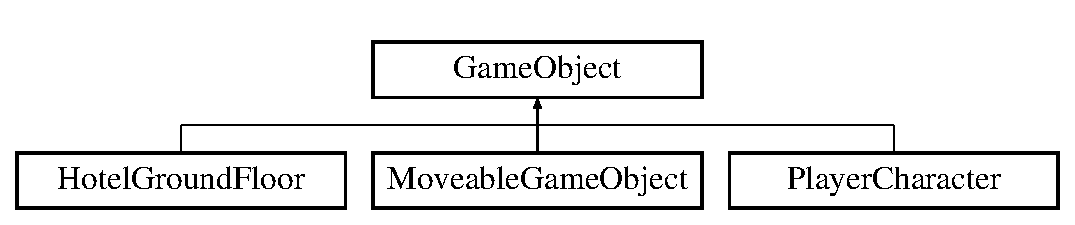
\includegraphics[height=2cm]{classGameObject}
\end{center}
\end{figure}
\subsection*{Public Member Functions}
\begin{DoxyCompactItemize}
\item 
\hyperlink{classGameObject_ad8d1bdb3864097a3723ddac03b947f95}{GameObject} (\hyperlink{classWorld}{World} $\ast$, CL\_\-Pointd \&, CL\_\-Angle \&)
\item 
void \hyperlink{classGameObject_a0eabb72240499a1878b420b5c3f0ecf3}{setDirection} (CL\_\-Angle \&)
\item 
CL\_\-Angle \hyperlink{classGameObject_a456901f9f0b261b206db248960633e50}{getDirection} (void)
\item 
void \hyperlink{classGameObject_a4fd1eeb91d5a220dde7b8574be19b651}{setPosition} (CL\_\-Pointd \&)
\item 
CL\_\-Pointd \hyperlink{classGameObject_adfc89f23ef6d0819c183f1c26bb27e58}{getPosition} (void)
\item 
virtual void \hyperlink{classGameObject_abb64143e72358beb808db22182517802}{draw} ()
\item 
virtual bool \hyperlink{classGameObject_ad2f3cd5d1f5a11b237507cd3ee98b95d}{update} (unsigned int)
\end{DoxyCompactItemize}
\subsection*{Protected Attributes}
\begin{DoxyCompactItemize}
\item 
\hypertarget{classGameObject_adce5bc0f31d7ce307f6bf8fe57030a24}{
\hyperlink{classWorld}{World} $\ast$ {\bfseries world}}
\label{classGameObject_adce5bc0f31d7ce307f6bf8fe57030a24}

\item 
\hypertarget{classGameObject_a9e3a44174a06dd260412d7a13d639d99}{
CL\_\-Pointd {\bfseries position}}
\label{classGameObject_a9e3a44174a06dd260412d7a13d639d99}

\item 
\hypertarget{classGameObject_a8df0dc007367b180dfcd9d2f193f6bdf}{
CL\_\-Angle {\bfseries direction}}
\label{classGameObject_a8df0dc007367b180dfcd9d2f193f6bdf}

\item 
\hypertarget{classGameObject_a5b841978ecf469bc3a69c0d05ad81013}{
CL\_\-Sprite $\ast$ {\bfseries static\_\-sprites} \mbox{[}8\mbox{]}}
\label{classGameObject_a5b841978ecf469bc3a69c0d05ad81013}

\item 
\hypertarget{classGameObject_a22464434abaabf3fb9aab0664dd22eb5}{
CL\_\-Sprite $\ast$ {\bfseries static\_\-current}}
\label{classGameObject_a22464434abaabf3fb9aab0664dd22eb5}

\end{DoxyCompactItemize}


\subsection{Constructor \& Destructor Documentation}
\hypertarget{classGameObject_ad8d1bdb3864097a3723ddac03b947f95}{
\index{GameObject@{GameObject}!GameObject@{GameObject}}
\index{GameObject@{GameObject}!GameObject@{GameObject}}
\subsubsection[{GameObject}]{\setlength{\rightskip}{0pt plus 5cm}GameObject::GameObject ({\bf World} $\ast$ {\em w}, \/  CL\_\-Pointd \& {\em initial\_\-position}, \/  CL\_\-Angle \& {\em initial\_\-direction})}}
\label{classGameObject_ad8d1bdb3864097a3723ddac03b947f95}
param w World$\ast$ param initial\_\-position CL\_\-Pointd The starting position in world coordinates. param initial\_\-direction CL\_\-Angle 

\subsection{Member Function Documentation}
\hypertarget{classGameObject_abb64143e72358beb808db22182517802}{
\index{GameObject@{GameObject}!draw@{draw}}
\index{draw@{draw}!GameObject@{GameObject}}
\subsubsection[{draw}]{\setlength{\rightskip}{0pt plus 5cm}void GameObject::draw (void)\hspace{0.3cm}{\ttfamily  \mbox{[}virtual\mbox{]}}}}
\label{classGameObject_abb64143e72358beb808db22182517802}
Draws the current static sprite for the object. 

Reimplemented in \hyperlink{classMoveableGameObject_a6110e3bcfb088cfaa53bc81ce220bab1}{MoveableGameObject}.\hypertarget{classGameObject_a456901f9f0b261b206db248960633e50}{
\index{GameObject@{GameObject}!getDirection@{getDirection}}
\index{getDirection@{getDirection}!GameObject@{GameObject}}
\subsubsection[{getDirection}]{\setlength{\rightskip}{0pt plus 5cm}CL\_\-Angle GameObject::getDirection (void)}}
\label{classGameObject_a456901f9f0b261b206db248960633e50}
Returns the angle. \hypertarget{classGameObject_adfc89f23ef6d0819c183f1c26bb27e58}{
\index{GameObject@{GameObject}!getPosition@{getPosition}}
\index{getPosition@{getPosition}!GameObject@{GameObject}}
\subsubsection[{getPosition}]{\setlength{\rightskip}{0pt plus 5cm}CL\_\-Pointd GameObject::getPosition (void)}}
\label{classGameObject_adfc89f23ef6d0819c183f1c26bb27e58}
Returns the position in world co-\/ordinates in CL\_\-Pointd. \hypertarget{classGameObject_a0eabb72240499a1878b420b5c3f0ecf3}{
\index{GameObject@{GameObject}!setDirection@{setDirection}}
\index{setDirection@{setDirection}!GameObject@{GameObject}}
\subsubsection[{setDirection}]{\setlength{\rightskip}{0pt plus 5cm}void GameObject::setDirection (CL\_\-Angle \& {\em new\_\-direction})}}
\label{classGameObject_a0eabb72240499a1878b420b5c3f0ecf3}
Sets the direction the game object is facing. This effects the sprite which is used when drawing it. \hypertarget{classGameObject_a4fd1eeb91d5a220dde7b8574be19b651}{
\index{GameObject@{GameObject}!setPosition@{setPosition}}
\index{setPosition@{setPosition}!GameObject@{GameObject}}
\subsubsection[{setPosition}]{\setlength{\rightskip}{0pt plus 5cm}void GameObject::setPosition (CL\_\-Pointd \& {\em new\_\-position})}}
\label{classGameObject_a4fd1eeb91d5a220dde7b8574be19b651}
Sets the position of the object.

param new\_\-position The position as CL\_\-Pointd in terms of world co-\/ordinates. \hypertarget{classGameObject_ad2f3cd5d1f5a11b237507cd3ee98b95d}{
\index{GameObject@{GameObject}!update@{update}}
\index{update@{update}!GameObject@{GameObject}}
\subsubsection[{update}]{\setlength{\rightskip}{0pt plus 5cm}bool GameObject::update (unsigned int {\em time\_\-elapsed\_\-ms})\hspace{0.3cm}{\ttfamily  \mbox{[}virtual\mbox{]}}}}
\label{classGameObject_ad2f3cd5d1f5a11b237507cd3ee98b95d}
Updates any animation in the current sprite. 

Reimplemented in \hyperlink{classMoveableGameObject_af2a5d981743e85b4bd35a90f874b361b}{MoveableGameObject}.

The documentation for this class was generated from the following files:\begin{DoxyCompactItemize}
\item 
source/game/\hyperlink{GameObject_8h}{GameObject.h}\item 
source/game/\hyperlink{GameObject_8cpp}{GameObject.cpp}\end{DoxyCompactItemize}

\hypertarget{classdlib_1_1graph}{
\section{dlib::graph$<$ T, E, mem\_\-manager $>$ Class Template Reference}
\label{classdlib_1_1graph}\index{dlib::graph@{dlib::graph}}
}
\subsection*{Public Types}
\begin{DoxyCompactItemize}
\item 
\hypertarget{classdlib_1_1graph_a1c448d65146aa8241a2ad6ce8c053b3c}{
typedef graph\_\-kernel\_\-1$<$ T, E, mem\_\-manager, false $>$ {\bfseries kernel\_\-1a}}
\label{classdlib_1_1graph_a1c448d65146aa8241a2ad6ce8c053b3c}

\item 
\hypertarget{classdlib_1_1graph_a271111ff39faae17c5ffd8547db3902f}{
typedef graph\_\-kernel\_\-1$<$ T, E, mem\_\-manager, true $>$ {\bfseries kernel\_\-1a\_\-c}}
\label{classdlib_1_1graph_a271111ff39faae17c5ffd8547db3902f}

\end{DoxyCompactItemize}
\subsubsection*{template$<$typename T, typename E = char, typename mem\_\-manager = memory\_\-manager$<$char$>$::kernel\_\-1a$>$ class dlib::graph$<$ T, E, mem\_\-manager $>$}



The documentation for this class was generated from the following file:\begin{DoxyCompactItemize}
\item 
source/dlib/graph.h\end{DoxyCompactItemize}

\hypertarget{structdlib_1_1grayscale__pixel__traits}{
\section{dlib::grayscale\_\-pixel\_\-traits$<$ T $>$ Struct Template Reference}
\label{structdlib_1_1grayscale__pixel__traits}\index{dlib::grayscale\_\-pixel\_\-traits@{dlib::grayscale\_\-pixel\_\-traits}}
}
\subsection*{Static Public Member Functions}
\begin{DoxyCompactItemize}
\item 
\hypertarget{structdlib_1_1grayscale__pixel__traits_a498037e5fe257a43cf4d900646a3451f}{
static unsigned long {\bfseries max} ()}
\label{structdlib_1_1grayscale__pixel__traits_a498037e5fe257a43cf4d900646a3451f}

\end{DoxyCompactItemize}
\subsection*{Static Public Attributes}
\begin{DoxyCompactItemize}
\item 
\hypertarget{structdlib_1_1grayscale__pixel__traits_ae1ca1f27ee5ac33dc13b098d55fbad28}{
static const bool {\bfseries rgb} = false}
\label{structdlib_1_1grayscale__pixel__traits_ae1ca1f27ee5ac33dc13b098d55fbad28}

\item 
\hypertarget{structdlib_1_1grayscale__pixel__traits_a2a6aa062e40b5849d9e3becc29c8e898}{
static const bool {\bfseries rgb\_\-alpha} = false}
\label{structdlib_1_1grayscale__pixel__traits_a2a6aa062e40b5849d9e3becc29c8e898}

\item 
\hypertarget{structdlib_1_1grayscale__pixel__traits_a741a2bcf1f18844c5c0d47d594c05668}{
static const bool {\bfseries grayscale} = true}
\label{structdlib_1_1grayscale__pixel__traits_a741a2bcf1f18844c5c0d47d594c05668}

\item 
\hypertarget{structdlib_1_1grayscale__pixel__traits_a82b6b7e872250b16aebf7e029a8b8867}{
static const bool {\bfseries hsi} = false}
\label{structdlib_1_1grayscale__pixel__traits_a82b6b7e872250b16aebf7e029a8b8867}

\item 
\hypertarget{structdlib_1_1grayscale__pixel__traits_a8dcc500361adf59ad544e6143137df5e}{
static const long {\bfseries num} = 1}
\label{structdlib_1_1grayscale__pixel__traits_a8dcc500361adf59ad544e6143137df5e}

\item 
\hypertarget{structdlib_1_1grayscale__pixel__traits_a65b0ab709cee0fcf3d5ef63a7d27802e}{
static const bool {\bfseries has\_\-alpha} = false}
\label{structdlib_1_1grayscale__pixel__traits_a65b0ab709cee0fcf3d5ef63a7d27802e}

\end{DoxyCompactItemize}
\subsubsection*{template$<$typename T$>$ struct dlib::grayscale\_\-pixel\_\-traits$<$ T $>$}



The documentation for this struct was generated from the following file:\begin{DoxyCompactItemize}
\item 
source/dlib/pixel.h\end{DoxyCompactItemize}

\hypertarget{classdlib_1_1gui__error}{
\section{dlib::gui\_\-error Class Reference}
\label{classdlib_1_1gui__error}\index{dlib::gui\_\-error@{dlib::gui\_\-error}}
}
Inheritance diagram for dlib::gui\_\-error::\begin{figure}[H]
\begin{center}
\leavevmode
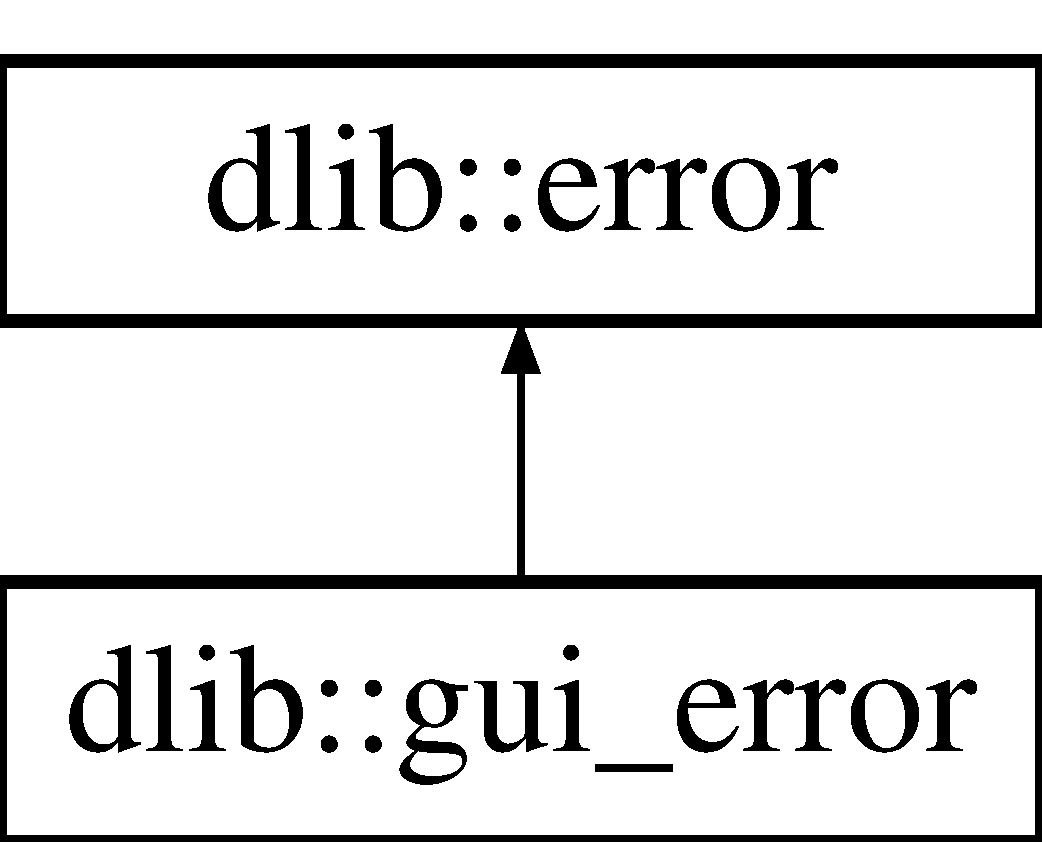
\includegraphics[height=2cm]{classdlib_1_1gui__error}
\end{center}
\end{figure}
\subsection*{Public Member Functions}
\begin{DoxyCompactItemize}
\item 
\hypertarget{classdlib_1_1gui__error_a77ec8eaf03541778946228b13be67564}{
{\bfseries gui\_\-error} (error\_\-type t, const std::string \&a)}
\label{classdlib_1_1gui__error_a77ec8eaf03541778946228b13be67564}

\item 
\hyperlink{classdlib_1_1gui__error_a79df44246d54d45905564cabd8ea0a6e}{gui\_\-error} (error\_\-type t)
\item 
\hyperlink{classdlib_1_1gui__error_a695fa7a02393b2154db455350fc9ab9c}{gui\_\-error} (const std::string \&a)
\item 
\hyperlink{classdlib_1_1gui__error_a12b91b87302cdcb3e727f4970b1f8453}{gui\_\-error} ()
\end{DoxyCompactItemize}


\subsection{Constructor \& Destructor Documentation}
\hypertarget{classdlib_1_1gui__error_a79df44246d54d45905564cabd8ea0a6e}{
\index{dlib::gui\_\-error@{dlib::gui\_\-error}!gui\_\-error@{gui\_\-error}}
\index{gui\_\-error@{gui\_\-error}!dlib::gui_error@{dlib::gui\_\-error}}
\subsubsection[{gui\_\-error}]{\setlength{\rightskip}{0pt plus 5cm}dlib::gui\_\-error::gui\_\-error (error\_\-type {\em t})\hspace{0.3cm}{\ttfamily  \mbox{[}inline\mbox{]}}}}
\label{classdlib_1_1gui__error_a79df44246d54d45905564cabd8ea0a6e}
ensures
\begin{DoxyItemize}
\item type == t
\item info == a ! 
\end{DoxyItemize}\hypertarget{classdlib_1_1gui__error_a695fa7a02393b2154db455350fc9ab9c}{
\index{dlib::gui\_\-error@{dlib::gui\_\-error}!gui\_\-error@{gui\_\-error}}
\index{gui\_\-error@{gui\_\-error}!dlib::gui_error@{dlib::gui\_\-error}}
\subsubsection[{gui\_\-error}]{\setlength{\rightskip}{0pt plus 5cm}dlib::gui\_\-error::gui\_\-error (const std::string \& {\em a})\hspace{0.3cm}{\ttfamily  \mbox{[}inline\mbox{]}}}}
\label{classdlib_1_1gui__error_a695fa7a02393b2154db455350fc9ab9c}
ensures
\begin{DoxyItemize}
\item type == t
\item info == \char`\"{}\char`\"{} ! 
\end{DoxyItemize}\hypertarget{classdlib_1_1gui__error_a12b91b87302cdcb3e727f4970b1f8453}{
\index{dlib::gui\_\-error@{dlib::gui\_\-error}!gui\_\-error@{gui\_\-error}}
\index{gui\_\-error@{gui\_\-error}!dlib::gui_error@{dlib::gui\_\-error}}
\subsubsection[{gui\_\-error}]{\setlength{\rightskip}{0pt plus 5cm}dlib::gui\_\-error::gui\_\-error ()\hspace{0.3cm}{\ttfamily  \mbox{[}inline\mbox{]}}}}
\label{classdlib_1_1gui__error_a12b91b87302cdcb3e727f4970b1f8453}
ensures
\begin{DoxyItemize}
\item type == EGUI
\item info == a ! 
\end{DoxyItemize}

The documentation for this class was generated from the following file:\begin{DoxyCompactItemize}
\item 
source/dlib/error.h\end{DoxyCompactItemize}

\hypertarget{classdlib_1_1hash__map}{
\section{dlib::hash\_\-map$<$ domain, range, expnum, mem\_\-manager, compare $>$ Class Template Reference}
\label{classdlib_1_1hash__map}\index{dlib::hash\_\-map@{dlib::hash\_\-map}}
}
\subsection*{Public Types}
\begin{DoxyCompactItemize}
\item 
\hypertarget{classdlib_1_1hash__map_a8eb280153ad2c7e79b47baaed73b7bd9}{
typedef hash\_\-map\_\-kernel\_\-1$<$ domain, range, expnum, hash\_\-table\_\-1, mem\_\-manager $>$ {\bfseries kernel\_\-1a}}
\label{classdlib_1_1hash__map_a8eb280153ad2c7e79b47baaed73b7bd9}

\item 
\hypertarget{classdlib_1_1hash__map_a15447377965b2d52de081028e7005024}{
typedef hash\_\-map\_\-kernel\_\-c$<$ kernel\_\-1a $>$ {\bfseries kernel\_\-1a\_\-c}}
\label{classdlib_1_1hash__map_a15447377965b2d52de081028e7005024}

\item 
\hypertarget{classdlib_1_1hash__map_aa3713b56d523e9539fc503442d727b52}{
typedef hash\_\-map\_\-kernel\_\-1$<$ domain, range, expnum, hash\_\-table\_\-2, mem\_\-manager $>$ {\bfseries kernel\_\-1b}}
\label{classdlib_1_1hash__map_aa3713b56d523e9539fc503442d727b52}

\item 
\hypertarget{classdlib_1_1hash__map_aa90abac9f060bb48036dec6e7d851e0f}{
typedef hash\_\-map\_\-kernel\_\-c$<$ kernel\_\-1b $>$ {\bfseries kernel\_\-1b\_\-c}}
\label{classdlib_1_1hash__map_aa90abac9f060bb48036dec6e7d851e0f}

\item 
\hypertarget{classdlib_1_1hash__map_a142a6f1b677afb755c6c2d0fcda09052}{
typedef hash\_\-map\_\-kernel\_\-1$<$ domain, range, expnum, hash\_\-table\_\-3, mem\_\-manager $>$ {\bfseries kernel\_\-1c}}
\label{classdlib_1_1hash__map_a142a6f1b677afb755c6c2d0fcda09052}

\item 
\hypertarget{classdlib_1_1hash__map_a405790287ae2018cb9249567256279b8}{
typedef hash\_\-map\_\-kernel\_\-c$<$ kernel\_\-1c $>$ {\bfseries kernel\_\-1c\_\-c}}
\label{classdlib_1_1hash__map_a405790287ae2018cb9249567256279b8}

\end{DoxyCompactItemize}
\subsubsection*{template$<$typename domain, typename range, unsigned long expnum, typename mem\_\-manager = memory\_\-manager$<$char$>$::kernel\_\-1a, typename compare = std::less$<$domain$>$$>$ class dlib::hash\_\-map$<$ domain, range, expnum, mem\_\-manager, compare $>$}



The documentation for this class was generated from the following file:\begin{DoxyCompactItemize}
\item 
source/dlib/hash\_\-map.h\end{DoxyCompactItemize}

\hypertarget{classdlib_1_1hash__set}{
\section{dlib::hash\_\-set$<$ T, expnum, mem\_\-manager, compare $>$ Class Template Reference}
\label{classdlib_1_1hash__set}\index{dlib::hash\_\-set@{dlib::hash\_\-set}}
}
\subsection*{Public Types}
\begin{DoxyCompactItemize}
\item 
\hypertarget{classdlib_1_1hash__set_af32d637e3ba29443f7099ac6b274752b}{
typedef hash\_\-set\_\-kernel\_\-1$<$ T, expnum, ht1a, mem\_\-manager $>$ {\bfseries kernel\_\-1a}}
\label{classdlib_1_1hash__set_af32d637e3ba29443f7099ac6b274752b}

\item 
\hypertarget{classdlib_1_1hash__set_a9f0e1de66982153d9c6a965fd911b0b5}{
typedef hash\_\-set\_\-kernel\_\-c$<$ kernel\_\-1a $>$ {\bfseries kernel\_\-1a\_\-c}}
\label{classdlib_1_1hash__set_a9f0e1de66982153d9c6a965fd911b0b5}

\item 
\hypertarget{classdlib_1_1hash__set_a828ff72e182e795aef43c5e3bbfb0609}{
typedef hash\_\-set\_\-kernel\_\-1$<$ T, expnum, ht2a, mem\_\-manager $>$ {\bfseries kernel\_\-1b}}
\label{classdlib_1_1hash__set_a828ff72e182e795aef43c5e3bbfb0609}

\item 
\hypertarget{classdlib_1_1hash__set_a7e63a3bbbb6238a5f8eac7608536078d}{
typedef hash\_\-set\_\-kernel\_\-c$<$ kernel\_\-1b $>$ {\bfseries kernel\_\-1b\_\-c}}
\label{classdlib_1_1hash__set_a7e63a3bbbb6238a5f8eac7608536078d}

\item 
\hypertarget{classdlib_1_1hash__set_a2d1375e7e537a0ecd2747d7e957ec8fa}{
typedef hash\_\-set\_\-kernel\_\-1$<$ T, expnum, ht2b, mem\_\-manager $>$ {\bfseries kernel\_\-1c}}
\label{classdlib_1_1hash__set_a2d1375e7e537a0ecd2747d7e957ec8fa}

\item 
\hypertarget{classdlib_1_1hash__set_a608c13e45f2a82f2579ce60ebc5bf86e}{
typedef hash\_\-set\_\-kernel\_\-c$<$ kernel\_\-1c $>$ {\bfseries kernel\_\-1c\_\-c}}
\label{classdlib_1_1hash__set_a608c13e45f2a82f2579ce60ebc5bf86e}

\end{DoxyCompactItemize}
\subsubsection*{template$<$typename T, unsigned long expnum, typename mem\_\-manager = memory\_\-manager$<$char$>$::kernel\_\-1a, typename compare = std::less$<$T$>$$>$ class dlib::hash\_\-set$<$ T, expnum, mem\_\-manager, compare $>$}



The documentation for this class was generated from the following file:\begin{DoxyCompactItemize}
\item 
source/dlib/hash\_\-set.h\end{DoxyCompactItemize}

\hypertarget{classdlib_1_1hash__table}{
\section{dlib::hash\_\-table$<$ domain, range, mem\_\-manager, compare $>$ Class Template Reference}
\label{classdlib_1_1hash__table}\index{dlib::hash\_\-table@{dlib::hash\_\-table}}
}
\subsection*{Public Types}
\begin{DoxyCompactItemize}
\item 
\hypertarget{classdlib_1_1hash__table_a31668ea5710017284a1d074e8ccd5504}{
typedef hash\_\-table\_\-kernel\_\-1$<$ domain, range, mem\_\-manager, compare $>$ {\bfseries kernel\_\-1a}}
\label{classdlib_1_1hash__table_a31668ea5710017284a1d074e8ccd5504}

\item 
\hypertarget{classdlib_1_1hash__table_ad6960dab7470258df610ab124cbbd34b}{
typedef hash\_\-table\_\-kernel\_\-c$<$ kernel\_\-1a $>$ {\bfseries kernel\_\-1a\_\-c}}
\label{classdlib_1_1hash__table_ad6960dab7470258df610ab124cbbd34b}

\item 
\hypertarget{classdlib_1_1hash__table_ae38f1a0190b7a141b0426bcf91e62976}{
typedef hash\_\-table\_\-kernel\_\-2$<$ domain, range, bst\_\-1, mem\_\-manager, compare $>$ {\bfseries kernel\_\-2a}}
\label{classdlib_1_1hash__table_ae38f1a0190b7a141b0426bcf91e62976}

\item 
\hypertarget{classdlib_1_1hash__table_ae904372c3be0de166a2cc84066dd61ed}{
typedef hash\_\-table\_\-kernel\_\-c$<$ kernel\_\-2a $>$ {\bfseries kernel\_\-2a\_\-c}}
\label{classdlib_1_1hash__table_ae904372c3be0de166a2cc84066dd61ed}

\item 
\hypertarget{classdlib_1_1hash__table_aa8d858865be3918b87e91e0ff52ede48}{
typedef hash\_\-table\_\-kernel\_\-2$<$ domain, range, bst\_\-2, mem\_\-manager, compare $>$ {\bfseries kernel\_\-2b}}
\label{classdlib_1_1hash__table_aa8d858865be3918b87e91e0ff52ede48}

\item 
\hypertarget{classdlib_1_1hash__table_a841b252e4fefbd8c638b7720773858d1}{
typedef hash\_\-table\_\-kernel\_\-c$<$ kernel\_\-2b $>$ {\bfseries kernel\_\-2b\_\-c}}
\label{classdlib_1_1hash__table_a841b252e4fefbd8c638b7720773858d1}

\end{DoxyCompactItemize}
\subsubsection*{template$<$typename domain, typename range, typename mem\_\-manager = memory\_\-manager$<$char$>$::kernel\_\-1a, typename compare = std::less$<$domain$>$$>$ class dlib::hash\_\-table$<$ domain, range, mem\_\-manager, compare $>$}



The documentation for this class was generated from the following file:\begin{DoxyCompactItemize}
\item 
source/dlib/hash\_\-table.h\end{DoxyCompactItemize}

\hypertarget{structdlib_1_1assign__pixel__helpers_1_1helper_3_01P_00_01P_00_01grayscale_00_01grayscale_01_4}{
\section{dlib::assign\_\-pixel\_\-helpers::helper$<$ P, P, grayscale, grayscale $>$ Struct Template Reference}
\label{structdlib_1_1assign__pixel__helpers_1_1helper_3_01P_00_01P_00_01grayscale_00_01grayscale_01_4}\index{dlib::assign\_\-pixel\_\-helpers::helper$<$ P, P, grayscale, grayscale $>$@{dlib::assign\_\-pixel\_\-helpers::helper$<$ P, P, grayscale, grayscale $>$}}
}
\subsection*{Static Public Member Functions}
\begin{DoxyCompactItemize}
\item 
\hypertarget{structdlib_1_1assign__pixel__helpers_1_1helper_3_01P_00_01P_00_01grayscale_00_01grayscale_01_4_a9cd5bcfdaa1f0a3037e6d863ab6e92c5}{
static void {\bfseries assign} (P \&dest, const P \&src)}
\label{structdlib_1_1assign__pixel__helpers_1_1helper_3_01P_00_01P_00_01grayscale_00_01grayscale_01_4_a9cd5bcfdaa1f0a3037e6d863ab6e92c5}

\end{DoxyCompactItemize}
\subsubsection*{template$<$typename P$>$ struct dlib::assign\_\-pixel\_\-helpers::helper$<$ P, P, grayscale, grayscale $>$}



The documentation for this struct was generated from the following file:\begin{DoxyCompactItemize}
\item 
source/dlib/pixel.h\end{DoxyCompactItemize}

\hypertarget{structdlib_1_1assign__pixel__helpers_1_1helper_3_01P1_00_01P2_00_01grayscale_00_01grayscale_01_4}{
\section{dlib::assign\_\-pixel\_\-helpers::helper$<$ P1, P2, grayscale, grayscale $>$ Struct Template Reference}
\label{structdlib_1_1assign__pixel__helpers_1_1helper_3_01P1_00_01P2_00_01grayscale_00_01grayscale_01_4}\index{dlib::assign\_\-pixel\_\-helpers::helper$<$ P1, P2, grayscale, grayscale $>$@{dlib::assign\_\-pixel\_\-helpers::helper$<$ P1, P2, grayscale, grayscale $>$}}
}
\subsection*{Static Public Member Functions}
\begin{DoxyCompactItemize}
\item 
\hypertarget{structdlib_1_1assign__pixel__helpers_1_1helper_3_01P1_00_01P2_00_01grayscale_00_01grayscale_01_4_a001417cca981b59106bc94d0988805c2}{
static void {\bfseries assign} (P1 \&dest, const P2 \&src)}
\label{structdlib_1_1assign__pixel__helpers_1_1helper_3_01P1_00_01P2_00_01grayscale_00_01grayscale_01_4_a001417cca981b59106bc94d0988805c2}

\end{DoxyCompactItemize}
\subsubsection*{template$<$typename P1, typename P2$>$ struct dlib::assign\_\-pixel\_\-helpers::helper$<$ P1, P2, grayscale, grayscale $>$}



The documentation for this struct was generated from the following file:\begin{DoxyCompactItemize}
\item 
source/dlib/pixel.h\end{DoxyCompactItemize}

\hypertarget{structdlib_1_1assign__pixel__helpers_1_1helper_3_01P1_00_01P2_00_01grayscale_00_01hsi_01_4}{
\section{dlib::assign\_\-pixel\_\-helpers::helper$<$ P1, P2, grayscale, hsi $>$ Struct Template Reference}
\label{structdlib_1_1assign__pixel__helpers_1_1helper_3_01P1_00_01P2_00_01grayscale_00_01hsi_01_4}\index{dlib::assign\_\-pixel\_\-helpers::helper$<$ P1, P2, grayscale, hsi $>$@{dlib::assign\_\-pixel\_\-helpers::helper$<$ P1, P2, grayscale, hsi $>$}}
}
\subsection*{Static Public Member Functions}
\begin{DoxyCompactItemize}
\item 
\hypertarget{structdlib_1_1assign__pixel__helpers_1_1helper_3_01P1_00_01P2_00_01grayscale_00_01hsi_01_4_af5a7ba3c1c06868c0f7b51e1eb7e47c3}{
static void {\bfseries assign} (P1 \&dest, const P2 \&src)}
\label{structdlib_1_1assign__pixel__helpers_1_1helper_3_01P1_00_01P2_00_01grayscale_00_01hsi_01_4_af5a7ba3c1c06868c0f7b51e1eb7e47c3}

\end{DoxyCompactItemize}
\subsubsection*{template$<$typename P1, typename P2$>$ struct dlib::assign\_\-pixel\_\-helpers::helper$<$ P1, P2, grayscale, hsi $>$}



The documentation for this struct was generated from the following file:\begin{DoxyCompactItemize}
\item 
source/dlib/pixel.h\end{DoxyCompactItemize}

\hypertarget{structdlib_1_1assign__pixel__helpers_1_1helper_3_01P1_00_01P2_00_01grayscale_00_01rgb_01_4}{
\section{dlib::assign\_\-pixel\_\-helpers::helper$<$ P1, P2, grayscale, rgb $>$ Struct Template Reference}
\label{structdlib_1_1assign__pixel__helpers_1_1helper_3_01P1_00_01P2_00_01grayscale_00_01rgb_01_4}\index{dlib::assign\_\-pixel\_\-helpers::helper$<$ P1, P2, grayscale, rgb $>$@{dlib::assign\_\-pixel\_\-helpers::helper$<$ P1, P2, grayscale, rgb $>$}}
}
\subsection*{Static Public Member Functions}
\begin{DoxyCompactItemize}
\item 
\hypertarget{structdlib_1_1assign__pixel__helpers_1_1helper_3_01P1_00_01P2_00_01grayscale_00_01rgb_01_4_a39a319abdeb5ff8a749d493c2e2e025b}{
static void {\bfseries assign} (P1 \&dest, const P2 \&src)}
\label{structdlib_1_1assign__pixel__helpers_1_1helper_3_01P1_00_01P2_00_01grayscale_00_01rgb_01_4_a39a319abdeb5ff8a749d493c2e2e025b}

\end{DoxyCompactItemize}
\subsubsection*{template$<$typename P1, typename P2$>$ struct dlib::assign\_\-pixel\_\-helpers::helper$<$ P1, P2, grayscale, rgb $>$}



The documentation for this struct was generated from the following file:\begin{DoxyCompactItemize}
\item 
source/dlib/pixel.h\end{DoxyCompactItemize}

\hypertarget{structdlib_1_1assign__pixel__helpers_1_1helper_3_01P1_00_01P2_00_01grayscale_00_01rgb__alpha_01_4}{
\section{dlib::assign\_\-pixel\_\-helpers::helper$<$ P1, P2, grayscale, rgb\_\-alpha $>$ Struct Template Reference}
\label{structdlib_1_1assign__pixel__helpers_1_1helper_3_01P1_00_01P2_00_01grayscale_00_01rgb__alpha_01_4}\index{dlib::assign\_\-pixel\_\-helpers::helper$<$ P1, P2, grayscale, rgb\_\-alpha $>$@{dlib::assign\_\-pixel\_\-helpers::helper$<$ P1, P2, grayscale, rgb\_\-alpha $>$}}
}
\subsection*{Static Public Member Functions}
\begin{DoxyCompactItemize}
\item 
\hypertarget{structdlib_1_1assign__pixel__helpers_1_1helper_3_01P1_00_01P2_00_01grayscale_00_01rgb__alpha_01_4_aceab20bb1b3748b3c8597a9afc40dd2a}{
static void {\bfseries assign} (P1 \&dest, const P2 \&src)}
\label{structdlib_1_1assign__pixel__helpers_1_1helper_3_01P1_00_01P2_00_01grayscale_00_01rgb__alpha_01_4_aceab20bb1b3748b3c8597a9afc40dd2a}

\end{DoxyCompactItemize}
\subsubsection*{template$<$typename P1, typename P2$>$ struct dlib::assign\_\-pixel\_\-helpers::helper$<$ P1, P2, grayscale, rgb\_\-alpha $>$}



The documentation for this struct was generated from the following file:\begin{DoxyCompactItemize}
\item 
source/dlib/pixel.h\end{DoxyCompactItemize}

\hypertarget{structdlib_1_1assign__pixel__helpers_1_1helper_3_01P1_00_01P2_00_01hsi_00_01grayscale_01_4}{
\section{dlib::assign\_\-pixel\_\-helpers::helper$<$ P1, P2, hsi, grayscale $>$ Struct Template Reference}
\label{structdlib_1_1assign__pixel__helpers_1_1helper_3_01P1_00_01P2_00_01hsi_00_01grayscale_01_4}\index{dlib::assign\_\-pixel\_\-helpers::helper$<$ P1, P2, hsi, grayscale $>$@{dlib::assign\_\-pixel\_\-helpers::helper$<$ P1, P2, hsi, grayscale $>$}}
}
\subsection*{Static Public Member Functions}
\begin{DoxyCompactItemize}
\item 
\hypertarget{structdlib_1_1assign__pixel__helpers_1_1helper_3_01P1_00_01P2_00_01hsi_00_01grayscale_01_4_a5b6e835faa29df34cd4cfc29e5da0580}{
static void {\bfseries assign} (P1 \&dest, const P2 \&src)}
\label{structdlib_1_1assign__pixel__helpers_1_1helper_3_01P1_00_01P2_00_01hsi_00_01grayscale_01_4_a5b6e835faa29df34cd4cfc29e5da0580}

\end{DoxyCompactItemize}
\subsubsection*{template$<$typename P1, typename P2$>$ struct dlib::assign\_\-pixel\_\-helpers::helper$<$ P1, P2, hsi, grayscale $>$}



The documentation for this struct was generated from the following file:\begin{DoxyCompactItemize}
\item 
source/dlib/pixel.h\end{DoxyCompactItemize}

\hypertarget{structdlib_1_1assign__pixel__helpers_1_1helper_3_01P1_00_01P2_00_01hsi_00_01hsi_01_4}{
\section{dlib::assign\_\-pixel\_\-helpers::helper$<$ P1, P2, hsi, hsi $>$ Struct Template Reference}
\label{structdlib_1_1assign__pixel__helpers_1_1helper_3_01P1_00_01P2_00_01hsi_00_01hsi_01_4}\index{dlib::assign\_\-pixel\_\-helpers::helper$<$ P1, P2, hsi, hsi $>$@{dlib::assign\_\-pixel\_\-helpers::helper$<$ P1, P2, hsi, hsi $>$}}
}
\subsection*{Static Public Member Functions}
\begin{DoxyCompactItemize}
\item 
\hypertarget{structdlib_1_1assign__pixel__helpers_1_1helper_3_01P1_00_01P2_00_01hsi_00_01hsi_01_4_ace19b7489b0e1c16787567b1d80d73b1}{
static void {\bfseries assign} (P1 \&dest, const P2 \&src)}
\label{structdlib_1_1assign__pixel__helpers_1_1helper_3_01P1_00_01P2_00_01hsi_00_01hsi_01_4_ace19b7489b0e1c16787567b1d80d73b1}

\end{DoxyCompactItemize}
\subsubsection*{template$<$typename P1, typename P2$>$ struct dlib::assign\_\-pixel\_\-helpers::helper$<$ P1, P2, hsi, hsi $>$}



The documentation for this struct was generated from the following file:\begin{DoxyCompactItemize}
\item 
source/dlib/pixel.h\end{DoxyCompactItemize}

\hypertarget{structdlib_1_1assign__pixel__helpers_1_1helper_3_01P1_00_01P2_00_01hsi_00_01rgb_01_4}{
\section{dlib::assign\_\-pixel\_\-helpers::helper$<$ P1, P2, hsi, rgb $>$ Struct Template Reference}
\label{structdlib_1_1assign__pixel__helpers_1_1helper_3_01P1_00_01P2_00_01hsi_00_01rgb_01_4}\index{dlib::assign\_\-pixel\_\-helpers::helper$<$ P1, P2, hsi, rgb $>$@{dlib::assign\_\-pixel\_\-helpers::helper$<$ P1, P2, hsi, rgb $>$}}
}
\subsection*{Static Public Member Functions}
\begin{DoxyCompactItemize}
\item 
\hypertarget{structdlib_1_1assign__pixel__helpers_1_1helper_3_01P1_00_01P2_00_01hsi_00_01rgb_01_4_af0ef95c3b1e16d299e3e26d260b8c951}{
static void {\bfseries assign} (P1 \&dest, const P2 \&src)}
\label{structdlib_1_1assign__pixel__helpers_1_1helper_3_01P1_00_01P2_00_01hsi_00_01rgb_01_4_af0ef95c3b1e16d299e3e26d260b8c951}

\end{DoxyCompactItemize}
\subsubsection*{template$<$typename P1, typename P2$>$ struct dlib::assign\_\-pixel\_\-helpers::helper$<$ P1, P2, hsi, rgb $>$}



The documentation for this struct was generated from the following file:\begin{DoxyCompactItemize}
\item 
source/dlib/pixel.h\end{DoxyCompactItemize}

\hypertarget{structdlib_1_1assign__pixel__helpers_1_1helper_3_01P1_00_01P2_00_01hsi_00_01rgb__alpha_01_4}{
\section{dlib::assign\_\-pixel\_\-helpers::helper$<$ P1, P2, hsi, rgb\_\-alpha $>$ Struct Template Reference}
\label{structdlib_1_1assign__pixel__helpers_1_1helper_3_01P1_00_01P2_00_01hsi_00_01rgb__alpha_01_4}\index{dlib::assign\_\-pixel\_\-helpers::helper$<$ P1, P2, hsi, rgb\_\-alpha $>$@{dlib::assign\_\-pixel\_\-helpers::helper$<$ P1, P2, hsi, rgb\_\-alpha $>$}}
}
\subsection*{Static Public Member Functions}
\begin{DoxyCompactItemize}
\item 
\hypertarget{structdlib_1_1assign__pixel__helpers_1_1helper_3_01P1_00_01P2_00_01hsi_00_01rgb__alpha_01_4_aacd84ca0877d26a152e1a3394938f3bf}{
static void {\bfseries assign} (P1 \&dest, const P2 \&src)}
\label{structdlib_1_1assign__pixel__helpers_1_1helper_3_01P1_00_01P2_00_01hsi_00_01rgb__alpha_01_4_aacd84ca0877d26a152e1a3394938f3bf}

\end{DoxyCompactItemize}
\subsubsection*{template$<$typename P1, typename P2$>$ struct dlib::assign\_\-pixel\_\-helpers::helper$<$ P1, P2, hsi, rgb\_\-alpha $>$}



The documentation for this struct was generated from the following file:\begin{DoxyCompactItemize}
\item 
source/dlib/pixel.h\end{DoxyCompactItemize}

\hypertarget{structdlib_1_1assign__pixel__helpers_1_1helper_3_01P1_00_01P2_00_01rgb_00_01grayscale_01_4}{
\section{dlib::assign\_\-pixel\_\-helpers::helper$<$ P1, P2, rgb, grayscale $>$ Struct Template Reference}
\label{structdlib_1_1assign__pixel__helpers_1_1helper_3_01P1_00_01P2_00_01rgb_00_01grayscale_01_4}\index{dlib::assign\_\-pixel\_\-helpers::helper$<$ P1, P2, rgb, grayscale $>$@{dlib::assign\_\-pixel\_\-helpers::helper$<$ P1, P2, rgb, grayscale $>$}}
}
\subsection*{Static Public Member Functions}
\begin{DoxyCompactItemize}
\item 
\hypertarget{structdlib_1_1assign__pixel__helpers_1_1helper_3_01P1_00_01P2_00_01rgb_00_01grayscale_01_4_aba80472ad450ba4d94fe2b471b888bdd}{
static void {\bfseries assign} (P1 \&dest, const P2 \&src)}
\label{structdlib_1_1assign__pixel__helpers_1_1helper_3_01P1_00_01P2_00_01rgb_00_01grayscale_01_4_aba80472ad450ba4d94fe2b471b888bdd}

\end{DoxyCompactItemize}
\subsubsection*{template$<$typename P1, typename P2$>$ struct dlib::assign\_\-pixel\_\-helpers::helper$<$ P1, P2, rgb, grayscale $>$}



The documentation for this struct was generated from the following file:\begin{DoxyCompactItemize}
\item 
source/dlib/pixel.h\end{DoxyCompactItemize}

\hypertarget{structdlib_1_1assign__pixel__helpers_1_1helper_3_01P1_00_01P2_00_01rgb_00_01hsi_01_4}{
\section{dlib::assign\_\-pixel\_\-helpers::helper$<$ P1, P2, rgb, hsi $>$ Struct Template Reference}
\label{structdlib_1_1assign__pixel__helpers_1_1helper_3_01P1_00_01P2_00_01rgb_00_01hsi_01_4}\index{dlib::assign\_\-pixel\_\-helpers::helper$<$ P1, P2, rgb, hsi $>$@{dlib::assign\_\-pixel\_\-helpers::helper$<$ P1, P2, rgb, hsi $>$}}
}
\subsection*{Static Public Member Functions}
\begin{DoxyCompactItemize}
\item 
\hypertarget{structdlib_1_1assign__pixel__helpers_1_1helper_3_01P1_00_01P2_00_01rgb_00_01hsi_01_4_a94425f76d31c38f3f239a47f121e81e6}{
static void {\bfseries assign} (P1 \&dest, const P2 \&src)}
\label{structdlib_1_1assign__pixel__helpers_1_1helper_3_01P1_00_01P2_00_01rgb_00_01hsi_01_4_a94425f76d31c38f3f239a47f121e81e6}

\end{DoxyCompactItemize}
\subsubsection*{template$<$typename P1, typename P2$>$ struct dlib::assign\_\-pixel\_\-helpers::helper$<$ P1, P2, rgb, hsi $>$}



The documentation for this struct was generated from the following file:\begin{DoxyCompactItemize}
\item 
source/dlib/pixel.h\end{DoxyCompactItemize}

\hypertarget{structdlib_1_1assign__pixel__helpers_1_1helper_3_01P1_00_01P2_00_01rgb_00_01rgb_01_4}{
\section{dlib::assign\_\-pixel\_\-helpers::helper$<$ P1, P2, rgb, rgb $>$ Struct Template Reference}
\label{structdlib_1_1assign__pixel__helpers_1_1helper_3_01P1_00_01P2_00_01rgb_00_01rgb_01_4}\index{dlib::assign\_\-pixel\_\-helpers::helper$<$ P1, P2, rgb, rgb $>$@{dlib::assign\_\-pixel\_\-helpers::helper$<$ P1, P2, rgb, rgb $>$}}
}
\subsection*{Static Public Member Functions}
\begin{DoxyCompactItemize}
\item 
\hypertarget{structdlib_1_1assign__pixel__helpers_1_1helper_3_01P1_00_01P2_00_01rgb_00_01rgb_01_4_a832b9ff21b629a9bffd3774d5332c3aa}{
static void {\bfseries assign} (P1 \&dest, const P2 \&src)}
\label{structdlib_1_1assign__pixel__helpers_1_1helper_3_01P1_00_01P2_00_01rgb_00_01rgb_01_4_a832b9ff21b629a9bffd3774d5332c3aa}

\end{DoxyCompactItemize}
\subsubsection*{template$<$typename P1, typename P2$>$ struct dlib::assign\_\-pixel\_\-helpers::helper$<$ P1, P2, rgb, rgb $>$}



The documentation for this struct was generated from the following file:\begin{DoxyCompactItemize}
\item 
source/dlib/pixel.h\end{DoxyCompactItemize}

\hypertarget{structdlib_1_1assign__pixel__helpers_1_1helper_3_01P1_00_01P2_00_01rgb_00_01rgb__alpha_01_4}{
\section{dlib::assign\_\-pixel\_\-helpers::helper$<$ P1, P2, rgb, rgb\_\-alpha $>$ Struct Template Reference}
\label{structdlib_1_1assign__pixel__helpers_1_1helper_3_01P1_00_01P2_00_01rgb_00_01rgb__alpha_01_4}\index{dlib::assign\_\-pixel\_\-helpers::helper$<$ P1, P2, rgb, rgb\_\-alpha $>$@{dlib::assign\_\-pixel\_\-helpers::helper$<$ P1, P2, rgb, rgb\_\-alpha $>$}}
}
\subsection*{Static Public Member Functions}
\begin{DoxyCompactItemize}
\item 
\hypertarget{structdlib_1_1assign__pixel__helpers_1_1helper_3_01P1_00_01P2_00_01rgb_00_01rgb__alpha_01_4_ad0f9a0bf5babf3419c7cabe5a54c8ee4}{
static void {\bfseries assign} (P1 \&dest, const P2 \&src)}
\label{structdlib_1_1assign__pixel__helpers_1_1helper_3_01P1_00_01P2_00_01rgb_00_01rgb__alpha_01_4_ad0f9a0bf5babf3419c7cabe5a54c8ee4}

\end{DoxyCompactItemize}
\subsubsection*{template$<$typename P1, typename P2$>$ struct dlib::assign\_\-pixel\_\-helpers::helper$<$ P1, P2, rgb, rgb\_\-alpha $>$}



The documentation for this struct was generated from the following file:\begin{DoxyCompactItemize}
\item 
source/dlib/pixel.h\end{DoxyCompactItemize}

\hypertarget{structdlib_1_1assign__pixel__helpers_1_1helper_3_01P1_00_01P2_00_01rgb__alpha_00_01grayscale_01_4}{
\section{dlib::assign\_\-pixel\_\-helpers::helper$<$ P1, P2, rgb\_\-alpha, grayscale $>$ Struct Template Reference}
\label{structdlib_1_1assign__pixel__helpers_1_1helper_3_01P1_00_01P2_00_01rgb__alpha_00_01grayscale_01_4}\index{dlib::assign\_\-pixel\_\-helpers::helper$<$ P1, P2, rgb\_\-alpha, grayscale $>$@{dlib::assign\_\-pixel\_\-helpers::helper$<$ P1, P2, rgb\_\-alpha, grayscale $>$}}
}
\subsection*{Static Public Member Functions}
\begin{DoxyCompactItemize}
\item 
\hypertarget{structdlib_1_1assign__pixel__helpers_1_1helper_3_01P1_00_01P2_00_01rgb__alpha_00_01grayscale_01_4_a157c3684cf23a7497a5375be7acc18c1}{
static void {\bfseries assign} (P1 \&dest, const P2 \&src)}
\label{structdlib_1_1assign__pixel__helpers_1_1helper_3_01P1_00_01P2_00_01rgb__alpha_00_01grayscale_01_4_a157c3684cf23a7497a5375be7acc18c1}

\end{DoxyCompactItemize}
\subsubsection*{template$<$typename P1, typename P2$>$ struct dlib::assign\_\-pixel\_\-helpers::helper$<$ P1, P2, rgb\_\-alpha, grayscale $>$}



The documentation for this struct was generated from the following file:\begin{DoxyCompactItemize}
\item 
source/dlib/pixel.h\end{DoxyCompactItemize}

\hypertarget{structdlib_1_1assign__pixel__helpers_1_1helper_3_01P1_00_01P2_00_01rgb__alpha_00_01hsi_01_4}{
\section{dlib::assign\_\-pixel\_\-helpers::helper$<$ P1, P2, rgb\_\-alpha, hsi $>$ Struct Template Reference}
\label{structdlib_1_1assign__pixel__helpers_1_1helper_3_01P1_00_01P2_00_01rgb__alpha_00_01hsi_01_4}\index{dlib::assign\_\-pixel\_\-helpers::helper$<$ P1, P2, rgb\_\-alpha, hsi $>$@{dlib::assign\_\-pixel\_\-helpers::helper$<$ P1, P2, rgb\_\-alpha, hsi $>$}}
}
\subsection*{Static Public Member Functions}
\begin{DoxyCompactItemize}
\item 
\hypertarget{structdlib_1_1assign__pixel__helpers_1_1helper_3_01P1_00_01P2_00_01rgb__alpha_00_01hsi_01_4_ac758e8f4e4bc79c10db8cec86658f495}{
static void {\bfseries assign} (P1 \&dest, const P2 \&src)}
\label{structdlib_1_1assign__pixel__helpers_1_1helper_3_01P1_00_01P2_00_01rgb__alpha_00_01hsi_01_4_ac758e8f4e4bc79c10db8cec86658f495}

\end{DoxyCompactItemize}
\subsubsection*{template$<$typename P1, typename P2$>$ struct dlib::assign\_\-pixel\_\-helpers::helper$<$ P1, P2, rgb\_\-alpha, hsi $>$}



The documentation for this struct was generated from the following file:\begin{DoxyCompactItemize}
\item 
source/dlib/pixel.h\end{DoxyCompactItemize}

\hypertarget{structdlib_1_1assign__pixel__helpers_1_1helper_3_01P1_00_01P2_00_01rgb__alpha_00_01rgb_01_4}{
\section{dlib::assign\_\-pixel\_\-helpers::helper$<$ P1, P2, rgb\_\-alpha, rgb $>$ Struct Template Reference}
\label{structdlib_1_1assign__pixel__helpers_1_1helper_3_01P1_00_01P2_00_01rgb__alpha_00_01rgb_01_4}\index{dlib::assign\_\-pixel\_\-helpers::helper$<$ P1, P2, rgb\_\-alpha, rgb $>$@{dlib::assign\_\-pixel\_\-helpers::helper$<$ P1, P2, rgb\_\-alpha, rgb $>$}}
}
\subsection*{Static Public Member Functions}
\begin{DoxyCompactItemize}
\item 
\hypertarget{structdlib_1_1assign__pixel__helpers_1_1helper_3_01P1_00_01P2_00_01rgb__alpha_00_01rgb_01_4_afc4b1d4643809daf63e5090d25bb121c}{
static void {\bfseries assign} (P1 \&dest, const P2 \&src)}
\label{structdlib_1_1assign__pixel__helpers_1_1helper_3_01P1_00_01P2_00_01rgb__alpha_00_01rgb_01_4_afc4b1d4643809daf63e5090d25bb121c}

\end{DoxyCompactItemize}
\subsubsection*{template$<$typename P1, typename P2$>$ struct dlib::assign\_\-pixel\_\-helpers::helper$<$ P1, P2, rgb\_\-alpha, rgb $>$}



The documentation for this struct was generated from the following file:\begin{DoxyCompactItemize}
\item 
source/dlib/pixel.h\end{DoxyCompactItemize}

\hypertarget{structdlib_1_1assign__pixel__helpers_1_1helper_3_01P1_00_01P2_00_01rgb__alpha_00_01rgb__alpha_01_4}{
\section{dlib::assign\_\-pixel\_\-helpers::helper$<$ P1, P2, rgb\_\-alpha, rgb\_\-alpha $>$ Struct Template Reference}
\label{structdlib_1_1assign__pixel__helpers_1_1helper_3_01P1_00_01P2_00_01rgb__alpha_00_01rgb__alpha_01_4}\index{dlib::assign\_\-pixel\_\-helpers::helper$<$ P1, P2, rgb\_\-alpha, rgb\_\-alpha $>$@{dlib::assign\_\-pixel\_\-helpers::helper$<$ P1, P2, rgb\_\-alpha, rgb\_\-alpha $>$}}
}
\subsection*{Static Public Member Functions}
\begin{DoxyCompactItemize}
\item 
\hypertarget{structdlib_1_1assign__pixel__helpers_1_1helper_3_01P1_00_01P2_00_01rgb__alpha_00_01rgb__alpha_01_4_aeb8edd2af51889ee0f6562f85f3a9b68}{
static void {\bfseries assign} (P1 \&dest, const P2 \&src)}
\label{structdlib_1_1assign__pixel__helpers_1_1helper_3_01P1_00_01P2_00_01rgb__alpha_00_01rgb__alpha_01_4_aeb8edd2af51889ee0f6562f85f3a9b68}

\end{DoxyCompactItemize}
\subsubsection*{template$<$typename P1, typename P2$>$ struct dlib::assign\_\-pixel\_\-helpers::helper$<$ P1, P2, rgb\_\-alpha, rgb\_\-alpha $>$}



The documentation for this struct was generated from the following file:\begin{DoxyCompactItemize}
\item 
source/dlib/pixel.h\end{DoxyCompactItemize}

\hypertarget{structdlib_1_1assign__pixel__helpers_1_1helper_3_01P1_00_01unsigned_01char_00_01hsi_00_01grayscale_01_4}{
\section{dlib::assign\_\-pixel\_\-helpers::helper$<$ P1, unsigned char, hsi, grayscale $>$ Struct Template Reference}
\label{structdlib_1_1assign__pixel__helpers_1_1helper_3_01P1_00_01unsigned_01char_00_01hsi_00_01grayscale_01_4}\index{dlib::assign\_\-pixel\_\-helpers::helper$<$ P1, unsigned char, hsi, grayscale $>$@{dlib::assign\_\-pixel\_\-helpers::helper$<$ P1, unsigned char, hsi, grayscale $>$}}
}
\subsection*{Static Public Member Functions}
\begin{DoxyCompactItemize}
\item 
\hypertarget{structdlib_1_1assign__pixel__helpers_1_1helper_3_01P1_00_01unsigned_01char_00_01hsi_00_01grayscale_01_4_a7b04f26ace3205e6da4133c0ea4f4c53}{
static void {\bfseries assign} (P1 \&dest, const unsigned char \&src)}
\label{structdlib_1_1assign__pixel__helpers_1_1helper_3_01P1_00_01unsigned_01char_00_01hsi_00_01grayscale_01_4_a7b04f26ace3205e6da4133c0ea4f4c53}

\end{DoxyCompactItemize}
\subsubsection*{template$<$typename P1$>$ struct dlib::assign\_\-pixel\_\-helpers::helper$<$ P1, unsigned char, hsi, grayscale $>$}



The documentation for this struct was generated from the following file:\begin{DoxyCompactItemize}
\item 
source/dlib/pixel.h\end{DoxyCompactItemize}

\hypertarget{structdlib_1_1assign__pixel__helpers_1_1helper_3_01P1_00_01unsigned_01char_00_01rgb_00_01grayscale_01_4}{
\section{dlib::assign\_\-pixel\_\-helpers::helper$<$ P1, unsigned char, rgb, grayscale $>$ Struct Template Reference}
\label{structdlib_1_1assign__pixel__helpers_1_1helper_3_01P1_00_01unsigned_01char_00_01rgb_00_01grayscale_01_4}\index{dlib::assign\_\-pixel\_\-helpers::helper$<$ P1, unsigned char, rgb, grayscale $>$@{dlib::assign\_\-pixel\_\-helpers::helper$<$ P1, unsigned char, rgb, grayscale $>$}}
}
\subsection*{Static Public Member Functions}
\begin{DoxyCompactItemize}
\item 
\hypertarget{structdlib_1_1assign__pixel__helpers_1_1helper_3_01P1_00_01unsigned_01char_00_01rgb_00_01grayscale_01_4_ad1b5e22580cc70d6132b205552327703}{
static void {\bfseries assign} (P1 \&dest, const unsigned char \&src)}
\label{structdlib_1_1assign__pixel__helpers_1_1helper_3_01P1_00_01unsigned_01char_00_01rgb_00_01grayscale_01_4_ad1b5e22580cc70d6132b205552327703}

\end{DoxyCompactItemize}
\subsubsection*{template$<$typename P1$>$ struct dlib::assign\_\-pixel\_\-helpers::helper$<$ P1, unsigned char, rgb, grayscale $>$}



The documentation for this struct was generated from the following file:\begin{DoxyCompactItemize}
\item 
source/dlib/pixel.h\end{DoxyCompactItemize}

\hypertarget{structdlib_1_1assign__pixel__helpers_1_1helper_3_01P1_00_01unsigned_01char_00_01rgb__alpha_00_01grayscale_01_4}{
\section{dlib::assign\_\-pixel\_\-helpers::helper$<$ P1, unsigned char, rgb\_\-alpha, grayscale $>$ Struct Template Reference}
\label{structdlib_1_1assign__pixel__helpers_1_1helper_3_01P1_00_01unsigned_01char_00_01rgb__alpha_00_01grayscale_01_4}\index{dlib::assign\_\-pixel\_\-helpers::helper$<$ P1, unsigned char, rgb\_\-alpha, grayscale $>$@{dlib::assign\_\-pixel\_\-helpers::helper$<$ P1, unsigned char, rgb\_\-alpha, grayscale $>$}}
}
\subsection*{Static Public Member Functions}
\begin{DoxyCompactItemize}
\item 
\hypertarget{structdlib_1_1assign__pixel__helpers_1_1helper_3_01P1_00_01unsigned_01char_00_01rgb__alpha_00_01grayscale_01_4_a5282b7adad404e5c0f0deaebde5cd4b9}{
static void {\bfseries assign} (P1 \&dest, const unsigned char \&src)}
\label{structdlib_1_1assign__pixel__helpers_1_1helper_3_01P1_00_01unsigned_01char_00_01rgb__alpha_00_01grayscale_01_4_a5282b7adad404e5c0f0deaebde5cd4b9}

\end{DoxyCompactItemize}
\subsubsection*{template$<$typename P1$>$ struct dlib::assign\_\-pixel\_\-helpers::helper$<$ P1, unsigned char, rgb\_\-alpha, grayscale $>$}



The documentation for this struct was generated from the following file:\begin{DoxyCompactItemize}
\item 
source/dlib/pixel.h\end{DoxyCompactItemize}

\hypertarget{structdlib_1_1hsi__pixel}{
\section{dlib::hsi\_\-pixel Struct Reference}
\label{structdlib_1_1hsi__pixel}\index{dlib::hsi\_\-pixel@{dlib::hsi\_\-pixel}}
}
\subsection*{Public Member Functions}
\begin{DoxyCompactItemize}
\item 
\hyperlink{structdlib_1_1hsi__pixel_a0c0e3a9cdcb8467326a256b897e1bd24}{hsi\_\-pixel} ()
\item 
\hypertarget{structdlib_1_1hsi__pixel_a46fe4b177588375562346727ba8f850e}{
{\bfseries hsi\_\-pixel} (unsigned char h\_\-, unsigned char s\_\-, unsigned char i\_\-)}
\label{structdlib_1_1hsi__pixel_a46fe4b177588375562346727ba8f850e}

\end{DoxyCompactItemize}
\subsection*{Public Attributes}
\begin{DoxyCompactItemize}
\item 
\hypertarget{structdlib_1_1hsi__pixel_af1db1e3a8cd094907b9c8304d3a8976b}{
unsigned char {\bfseries h}}
\label{structdlib_1_1hsi__pixel_af1db1e3a8cd094907b9c8304d3a8976b}

\item 
\hypertarget{structdlib_1_1hsi__pixel_acd183911f61c335fcac35d429bdf33da}{
unsigned char {\bfseries s}}
\label{structdlib_1_1hsi__pixel_acd183911f61c335fcac35d429bdf33da}

\item 
\hypertarget{structdlib_1_1hsi__pixel_a541e836f07fd6d3b9425e45e291e2f8b}{
unsigned char {\bfseries i}}
\label{structdlib_1_1hsi__pixel_a541e836f07fd6d3b9425e45e291e2f8b}

\end{DoxyCompactItemize}


\subsection{Constructor \& Destructor Documentation}
\hypertarget{structdlib_1_1hsi__pixel_a0c0e3a9cdcb8467326a256b897e1bd24}{
\index{dlib::hsi\_\-pixel@{dlib::hsi\_\-pixel}!hsi\_\-pixel@{hsi\_\-pixel}}
\index{hsi\_\-pixel@{hsi\_\-pixel}!dlib::hsi_pixel@{dlib::hsi\_\-pixel}}
\subsubsection[{hsi\_\-pixel}]{\setlength{\rightskip}{0pt plus 5cm}dlib::hsi\_\-pixel::hsi\_\-pixel ()\hspace{0.3cm}{\ttfamily  \mbox{[}inline\mbox{]}}}}
\label{structdlib_1_1hsi__pixel_a0c0e3a9cdcb8467326a256b897e1bd24}
WHAT THIS OBJECT REPRESENTS This is a simple struct that represents an HSI colored graphical pixel. ! 

The documentation for this struct was generated from the following file:\begin{DoxyCompactItemize}
\item 
source/dlib/pixel.h\end{DoxyCompactItemize}

\hypertarget{structdlib_1_1assign__pixel__helpers_1_1HSL}{
\section{dlib::assign\_\-pixel\_\-helpers::HSL Struct Reference}
\label{structdlib_1_1assign__pixel__helpers_1_1HSL}\index{dlib::assign\_\-pixel\_\-helpers::HSL@{dlib::assign\_\-pixel\_\-helpers::HSL}}
}
\subsection*{Public Attributes}
\begin{DoxyCompactItemize}
\item 
\hypertarget{structdlib_1_1assign__pixel__helpers_1_1HSL_a708cf7ee55919d08a3cbe0019685ba55}{
double {\bfseries h}}
\label{structdlib_1_1assign__pixel__helpers_1_1HSL_a708cf7ee55919d08a3cbe0019685ba55}

\item 
\hypertarget{structdlib_1_1assign__pixel__helpers_1_1HSL_a51055d41b09bc3d89f63eb00ba4789e7}{
double {\bfseries s}}
\label{structdlib_1_1assign__pixel__helpers_1_1HSL_a51055d41b09bc3d89f63eb00ba4789e7}

\item 
\hypertarget{structdlib_1_1assign__pixel__helpers_1_1HSL_a4f9c90fb7bac1cb003edd7e8da974c1f}{
double {\bfseries l}}
\label{structdlib_1_1assign__pixel__helpers_1_1HSL_a4f9c90fb7bac1cb003edd7e8da974c1f}

\end{DoxyCompactItemize}


The documentation for this struct was generated from the following file:\begin{DoxyCompactItemize}
\item 
source/dlib/pixel.h\end{DoxyCompactItemize}

\hypertarget{structdlib_1_1is__built__in__scalar__type}{
\section{dlib::is\_\-built\_\-in\_\-scalar\_\-type$<$ T $>$ Struct Template Reference}
\label{structdlib_1_1is__built__in__scalar__type}\index{dlib::is\_\-built\_\-in\_\-scalar\_\-type@{dlib::is\_\-built\_\-in\_\-scalar\_\-type}}
}


{\ttfamily \#include $<$algs.h$>$}\subsection*{Static Public Attributes}
\begin{DoxyCompactItemize}
\item 
\hypertarget{structdlib_1_1is__built__in__scalar__type_a25f19ea2e573cc6e32ee7f7e5b0ea0bc}{
static const bool {\bfseries value} = false}
\label{structdlib_1_1is__built__in__scalar__type_a25f19ea2e573cc6e32ee7f7e5b0ea0bc}

\end{DoxyCompactItemize}


\subsection{Detailed Description}
\subsubsection*{template$<$typename T$>$ struct dlib::is\_\-built\_\-in\_\-scalar\_\-type$<$ T $>$}

A \hyperlink{structdlib_1_1is__built__in__scalar__type}{is\_\-built\_\-in\_\-scalar\_\-type}

This is a template that allows you to determine if the given type is a built in scalar type such as an int, char, float, short, etc...

For example, is\_\-built\_\-in\_\-scalar\_\-type$<$char$>$::value == true For example, is\_\-built\_\-in\_\-scalar\_\-type$<$std::string$>$::value == false ! 

The documentation for this struct was generated from the following file:\begin{DoxyCompactItemize}
\item 
source/dlib/algs.h\end{DoxyCompactItemize}

\hypertarget{structdlib_1_1is__built__in__scalar__type_3_01char_01_4}{
\section{dlib::is\_\-built\_\-in\_\-scalar\_\-type$<$ char $>$ Struct Template Reference}
\label{structdlib_1_1is__built__in__scalar__type_3_01char_01_4}\index{dlib::is\_\-built\_\-in\_\-scalar\_\-type$<$ char $>$@{dlib::is\_\-built\_\-in\_\-scalar\_\-type$<$ char $>$}}
}
\subsection*{Static Public Attributes}
\begin{DoxyCompactItemize}
\item 
\hypertarget{structdlib_1_1is__built__in__scalar__type_3_01char_01_4_a44f76ad3840e087faa28e5d05a2c491b}{
static const bool {\bfseries value} = true}
\label{structdlib_1_1is__built__in__scalar__type_3_01char_01_4_a44f76ad3840e087faa28e5d05a2c491b}

\end{DoxyCompactItemize}
\subsubsection*{template$<$$>$ struct dlib::is\_\-built\_\-in\_\-scalar\_\-type$<$ char $>$}



The documentation for this struct was generated from the following file:\begin{DoxyCompactItemize}
\item 
source/dlib/algs.h\end{DoxyCompactItemize}

\hypertarget{structdlib_1_1is__built__in__scalar__type_3_01double_01_4}{
\section{dlib::is\_\-built\_\-in\_\-scalar\_\-type$<$ double $>$ Struct Template Reference}
\label{structdlib_1_1is__built__in__scalar__type_3_01double_01_4}\index{dlib::is\_\-built\_\-in\_\-scalar\_\-type$<$ double $>$@{dlib::is\_\-built\_\-in\_\-scalar\_\-type$<$ double $>$}}
}
\subsection*{Static Public Attributes}
\begin{DoxyCompactItemize}
\item 
\hypertarget{structdlib_1_1is__built__in__scalar__type_3_01double_01_4_a7b6873f42f78049c4fd84d7418fe03bf}{
static const bool {\bfseries value} = true}
\label{structdlib_1_1is__built__in__scalar__type_3_01double_01_4_a7b6873f42f78049c4fd84d7418fe03bf}

\end{DoxyCompactItemize}
\subsubsection*{template$<$$>$ struct dlib::is\_\-built\_\-in\_\-scalar\_\-type$<$ double $>$}



The documentation for this struct was generated from the following file:\begin{DoxyCompactItemize}
\item 
source/dlib/algs.h\end{DoxyCompactItemize}

\hypertarget{structdlib_1_1is__built__in__scalar__type_3_01float_01_4}{
\section{dlib::is\_\-built\_\-in\_\-scalar\_\-type$<$ float $>$ Struct Template Reference}
\label{structdlib_1_1is__built__in__scalar__type_3_01float_01_4}\index{dlib::is\_\-built\_\-in\_\-scalar\_\-type$<$ float $>$@{dlib::is\_\-built\_\-in\_\-scalar\_\-type$<$ float $>$}}
}
\subsection*{Static Public Attributes}
\begin{DoxyCompactItemize}
\item 
\hypertarget{structdlib_1_1is__built__in__scalar__type_3_01float_01_4_a28caeead3cc65760f388d23bd6f2fe14}{
static const bool {\bfseries value} = true}
\label{structdlib_1_1is__built__in__scalar__type_3_01float_01_4_a28caeead3cc65760f388d23bd6f2fe14}

\end{DoxyCompactItemize}
\subsubsection*{template$<$$>$ struct dlib::is\_\-built\_\-in\_\-scalar\_\-type$<$ float $>$}



The documentation for this struct was generated from the following file:\begin{DoxyCompactItemize}
\item 
source/dlib/algs.h\end{DoxyCompactItemize}

\hypertarget{structdlib_1_1is__built__in__scalar__type_3_01int_01_4}{
\section{dlib::is\_\-built\_\-in\_\-scalar\_\-type$<$ int $>$ Struct Template Reference}
\label{structdlib_1_1is__built__in__scalar__type_3_01int_01_4}\index{dlib::is\_\-built\_\-in\_\-scalar\_\-type$<$ int $>$@{dlib::is\_\-built\_\-in\_\-scalar\_\-type$<$ int $>$}}
}
\subsection*{Static Public Attributes}
\begin{DoxyCompactItemize}
\item 
\hypertarget{structdlib_1_1is__built__in__scalar__type_3_01int_01_4_a1af5d205e0ebc75014277a29000f78fc}{
static const bool {\bfseries value} = true}
\label{structdlib_1_1is__built__in__scalar__type_3_01int_01_4_a1af5d205e0ebc75014277a29000f78fc}

\end{DoxyCompactItemize}
\subsubsection*{template$<$$>$ struct dlib::is\_\-built\_\-in\_\-scalar\_\-type$<$ int $>$}



The documentation for this struct was generated from the following file:\begin{DoxyCompactItemize}
\item 
source/dlib/algs.h\end{DoxyCompactItemize}

\hypertarget{structdlib_1_1is__built__in__scalar__type_3_01long_01_4}{
\section{dlib::is\_\-built\_\-in\_\-scalar\_\-type$<$ long $>$ Struct Template Reference}
\label{structdlib_1_1is__built__in__scalar__type_3_01long_01_4}\index{dlib::is\_\-built\_\-in\_\-scalar\_\-type$<$ long $>$@{dlib::is\_\-built\_\-in\_\-scalar\_\-type$<$ long $>$}}
}
\subsection*{Static Public Attributes}
\begin{DoxyCompactItemize}
\item 
\hypertarget{structdlib_1_1is__built__in__scalar__type_3_01long_01_4_a07e6730fe56ee02bcb0445a5595d4872}{
static const bool {\bfseries value} = true}
\label{structdlib_1_1is__built__in__scalar__type_3_01long_01_4_a07e6730fe56ee02bcb0445a5595d4872}

\end{DoxyCompactItemize}
\subsubsection*{template$<$$>$ struct dlib::is\_\-built\_\-in\_\-scalar\_\-type$<$ long $>$}



The documentation for this struct was generated from the following file:\begin{DoxyCompactItemize}
\item 
source/dlib/algs.h\end{DoxyCompactItemize}

\hypertarget{structdlib_1_1is__built__in__scalar__type_3_01long_01double_01_4}{
\section{dlib::is\_\-built\_\-in\_\-scalar\_\-type$<$ long double $>$ Struct Template Reference}
\label{structdlib_1_1is__built__in__scalar__type_3_01long_01double_01_4}\index{dlib::is\_\-built\_\-in\_\-scalar\_\-type$<$ long double $>$@{dlib::is\_\-built\_\-in\_\-scalar\_\-type$<$ long double $>$}}
}
\subsection*{Static Public Attributes}
\begin{DoxyCompactItemize}
\item 
\hypertarget{structdlib_1_1is__built__in__scalar__type_3_01long_01double_01_4_a8fd91a93b141f0ce4b27ce2a3e97bb0c}{
static const bool {\bfseries value} = true}
\label{structdlib_1_1is__built__in__scalar__type_3_01long_01double_01_4_a8fd91a93b141f0ce4b27ce2a3e97bb0c}

\end{DoxyCompactItemize}
\subsubsection*{template$<$$>$ struct dlib::is\_\-built\_\-in\_\-scalar\_\-type$<$ long double $>$}



The documentation for this struct was generated from the following file:\begin{DoxyCompactItemize}
\item 
source/dlib/algs.h\end{DoxyCompactItemize}

\hypertarget{structdlib_1_1is__built__in__scalar__type_3_01short_01_4}{
\section{dlib::is\_\-built\_\-in\_\-scalar\_\-type$<$ short $>$ Struct Template Reference}
\label{structdlib_1_1is__built__in__scalar__type_3_01short_01_4}\index{dlib::is\_\-built\_\-in\_\-scalar\_\-type$<$ short $>$@{dlib::is\_\-built\_\-in\_\-scalar\_\-type$<$ short $>$}}
}
\subsection*{Static Public Attributes}
\begin{DoxyCompactItemize}
\item 
\hypertarget{structdlib_1_1is__built__in__scalar__type_3_01short_01_4_a6959fdd1c59e7f0b28ed9a8d18f4c550}{
static const bool {\bfseries value} = true}
\label{structdlib_1_1is__built__in__scalar__type_3_01short_01_4_a6959fdd1c59e7f0b28ed9a8d18f4c550}

\end{DoxyCompactItemize}
\subsubsection*{template$<$$>$ struct dlib::is\_\-built\_\-in\_\-scalar\_\-type$<$ short $>$}



The documentation for this struct was generated from the following file:\begin{DoxyCompactItemize}
\item 
source/dlib/algs.h\end{DoxyCompactItemize}

\hypertarget{structdlib_1_1is__built__in__scalar__type_3_01signed_01char_01_4}{
\section{dlib::is\_\-built\_\-in\_\-scalar\_\-type$<$ signed char $>$ Struct Template Reference}
\label{structdlib_1_1is__built__in__scalar__type_3_01signed_01char_01_4}\index{dlib::is\_\-built\_\-in\_\-scalar\_\-type$<$ signed char $>$@{dlib::is\_\-built\_\-in\_\-scalar\_\-type$<$ signed char $>$}}
}
\subsection*{Static Public Attributes}
\begin{DoxyCompactItemize}
\item 
\hypertarget{structdlib_1_1is__built__in__scalar__type_3_01signed_01char_01_4_ab9e5755879587c595c64c68ade6c96e2}{
static const bool {\bfseries value} = true}
\label{structdlib_1_1is__built__in__scalar__type_3_01signed_01char_01_4_ab9e5755879587c595c64c68ade6c96e2}

\end{DoxyCompactItemize}
\subsubsection*{template$<$$>$ struct dlib::is\_\-built\_\-in\_\-scalar\_\-type$<$ signed char $>$}



The documentation for this struct was generated from the following file:\begin{DoxyCompactItemize}
\item 
source/dlib/algs.h\end{DoxyCompactItemize}

\hypertarget{structdlib_1_1is__built__in__scalar__type_3_01uint64_01_4}{
\section{dlib::is\_\-built\_\-in\_\-scalar\_\-type$<$ uint64 $>$ Struct Template Reference}
\label{structdlib_1_1is__built__in__scalar__type_3_01uint64_01_4}\index{dlib::is\_\-built\_\-in\_\-scalar\_\-type$<$ uint64 $>$@{dlib::is\_\-built\_\-in\_\-scalar\_\-type$<$ uint64 $>$}}
}
\subsection*{Static Public Attributes}
\begin{DoxyCompactItemize}
\item 
\hypertarget{structdlib_1_1is__built__in__scalar__type_3_01uint64_01_4_ad3e33339cc71c9116f070cd7e1c49e31}{
static const bool {\bfseries value} = true}
\label{structdlib_1_1is__built__in__scalar__type_3_01uint64_01_4_ad3e33339cc71c9116f070cd7e1c49e31}

\end{DoxyCompactItemize}
\subsubsection*{template$<$$>$ struct dlib::is\_\-built\_\-in\_\-scalar\_\-type$<$ uint64 $>$}



The documentation for this struct was generated from the following file:\begin{DoxyCompactItemize}
\item 
source/dlib/algs.h\end{DoxyCompactItemize}

\hypertarget{structdlib_1_1is__built__in__scalar__type_3_01unsigned_01char_01_4}{
\section{dlib::is\_\-built\_\-in\_\-scalar\_\-type$<$ unsigned char $>$ Struct Template Reference}
\label{structdlib_1_1is__built__in__scalar__type_3_01unsigned_01char_01_4}\index{dlib::is\_\-built\_\-in\_\-scalar\_\-type$<$ unsigned char $>$@{dlib::is\_\-built\_\-in\_\-scalar\_\-type$<$ unsigned char $>$}}
}
\subsection*{Static Public Attributes}
\begin{DoxyCompactItemize}
\item 
\hypertarget{structdlib_1_1is__built__in__scalar__type_3_01unsigned_01char_01_4_a96d55540506365cf76fc0d61eb93357f}{
static const bool {\bfseries value} = true}
\label{structdlib_1_1is__built__in__scalar__type_3_01unsigned_01char_01_4_a96d55540506365cf76fc0d61eb93357f}

\end{DoxyCompactItemize}
\subsubsection*{template$<$$>$ struct dlib::is\_\-built\_\-in\_\-scalar\_\-type$<$ unsigned char $>$}



The documentation for this struct was generated from the following file:\begin{DoxyCompactItemize}
\item 
source/dlib/algs.h\end{DoxyCompactItemize}

\hypertarget{structdlib_1_1is__built__in__scalar__type_3_01unsigned_01int_01_4}{
\section{dlib::is\_\-built\_\-in\_\-scalar\_\-type$<$ unsigned int $>$ Struct Template Reference}
\label{structdlib_1_1is__built__in__scalar__type_3_01unsigned_01int_01_4}\index{dlib::is\_\-built\_\-in\_\-scalar\_\-type$<$ unsigned int $>$@{dlib::is\_\-built\_\-in\_\-scalar\_\-type$<$ unsigned int $>$}}
}
\subsection*{Static Public Attributes}
\begin{DoxyCompactItemize}
\item 
\hypertarget{structdlib_1_1is__built__in__scalar__type_3_01unsigned_01int_01_4_a682e2695ed7279d5c532359a6c403c0b}{
static const bool {\bfseries value} = true}
\label{structdlib_1_1is__built__in__scalar__type_3_01unsigned_01int_01_4_a682e2695ed7279d5c532359a6c403c0b}

\end{DoxyCompactItemize}
\subsubsection*{template$<$$>$ struct dlib::is\_\-built\_\-in\_\-scalar\_\-type$<$ unsigned int $>$}



The documentation for this struct was generated from the following file:\begin{DoxyCompactItemize}
\item 
source/dlib/algs.h\end{DoxyCompactItemize}

\hypertarget{structdlib_1_1is__built__in__scalar__type_3_01unsigned_01long_01_4}{
\section{dlib::is\_\-built\_\-in\_\-scalar\_\-type$<$ unsigned long $>$ Struct Template Reference}
\label{structdlib_1_1is__built__in__scalar__type_3_01unsigned_01long_01_4}\index{dlib::is\_\-built\_\-in\_\-scalar\_\-type$<$ unsigned long $>$@{dlib::is\_\-built\_\-in\_\-scalar\_\-type$<$ unsigned long $>$}}
}
\subsection*{Static Public Attributes}
\begin{DoxyCompactItemize}
\item 
\hypertarget{structdlib_1_1is__built__in__scalar__type_3_01unsigned_01long_01_4_a58139b9f5dcfdac9b85ba9f1e73a9149}{
static const bool {\bfseries value} = true}
\label{structdlib_1_1is__built__in__scalar__type_3_01unsigned_01long_01_4_a58139b9f5dcfdac9b85ba9f1e73a9149}

\end{DoxyCompactItemize}
\subsubsection*{template$<$$>$ struct dlib::is\_\-built\_\-in\_\-scalar\_\-type$<$ unsigned long $>$}



The documentation for this struct was generated from the following file:\begin{DoxyCompactItemize}
\item 
source/dlib/algs.h\end{DoxyCompactItemize}

\hypertarget{structdlib_1_1is__built__in__scalar__type_3_01unsigned_01short_01_4}{
\section{dlib::is\_\-built\_\-in\_\-scalar\_\-type$<$ unsigned short $>$ Struct Template Reference}
\label{structdlib_1_1is__built__in__scalar__type_3_01unsigned_01short_01_4}\index{dlib::is\_\-built\_\-in\_\-scalar\_\-type$<$ unsigned short $>$@{dlib::is\_\-built\_\-in\_\-scalar\_\-type$<$ unsigned short $>$}}
}
\subsection*{Static Public Attributes}
\begin{DoxyCompactItemize}
\item 
\hypertarget{structdlib_1_1is__built__in__scalar__type_3_01unsigned_01short_01_4_a3444459f0318333fb407e3acadcee5ae}{
static const bool {\bfseries value} = true}
\label{structdlib_1_1is__built__in__scalar__type_3_01unsigned_01short_01_4_a3444459f0318333fb407e3acadcee5ae}

\end{DoxyCompactItemize}
\subsubsection*{template$<$$>$ struct dlib::is\_\-built\_\-in\_\-scalar\_\-type$<$ unsigned short $>$}



The documentation for this struct was generated from the following file:\begin{DoxyCompactItemize}
\item 
source/dlib/algs.h\end{DoxyCompactItemize}

\hypertarget{structdlib_1_1is__built__in__scalar__type_3_01wchar__t_01_4}{
\section{dlib::is\_\-built\_\-in\_\-scalar\_\-type$<$ wchar\_\-t $>$ Struct Template Reference}
\label{structdlib_1_1is__built__in__scalar__type_3_01wchar__t_01_4}\index{dlib::is\_\-built\_\-in\_\-scalar\_\-type$<$ wchar\_\-t $>$@{dlib::is\_\-built\_\-in\_\-scalar\_\-type$<$ wchar\_\-t $>$}}
}
\subsection*{Static Public Attributes}
\begin{DoxyCompactItemize}
\item 
\hypertarget{structdlib_1_1is__built__in__scalar__type_3_01wchar__t_01_4_afd71d33e4d414298b06e20fd3fc1d6c2}{
static const bool {\bfseries value} = true}
\label{structdlib_1_1is__built__in__scalar__type_3_01wchar__t_01_4_afd71d33e4d414298b06e20fd3fc1d6c2}

\end{DoxyCompactItemize}
\subsubsection*{template$<$$>$ struct dlib::is\_\-built\_\-in\_\-scalar\_\-type$<$ wchar\_\-t $>$}



The documentation for this struct was generated from the following file:\begin{DoxyCompactItemize}
\item 
source/dlib/algs.h\end{DoxyCompactItemize}

\hypertarget{structdlib_1_1is__const__type}{
\section{dlib::is\_\-const\_\-type$<$ T $>$ Struct Template Reference}
\label{structdlib_1_1is__const__type}\index{dlib::is\_\-const\_\-type@{dlib::is\_\-const\_\-type}}
}


{\ttfamily \#include $<$algs.h$>$}\subsection*{Static Public Attributes}
\begin{DoxyCompactItemize}
\item 
\hypertarget{structdlib_1_1is__const__type_a14ab4b30a04eecf9108c5a8f898fcb22}{
static const bool {\bfseries value} = false}
\label{structdlib_1_1is__const__type_a14ab4b30a04eecf9108c5a8f898fcb22}

\end{DoxyCompactItemize}


\subsection{Detailed Description}
\subsubsection*{template$<$typename T$>$ struct dlib::is\_\-const\_\-type$<$ T $>$}

A \hyperlink{structdlib_1_1is__const__type}{is\_\-const\_\-type}

This is a template where is\_\-const\_\-type$<$T$>$::value == true when T is a const type ane false otherwise. ! 

The documentation for this struct was generated from the following file:\begin{DoxyCompactItemize}
\item 
source/dlib/algs.h\end{DoxyCompactItemize}

\hypertarget{structdlib_1_1is__const__type_3_01const_01T_01_4}{
\section{dlib::is\_\-const\_\-type$<$ const T $>$ Struct Template Reference}
\label{structdlib_1_1is__const__type_3_01const_01T_01_4}\index{dlib::is\_\-const\_\-type$<$ const T $>$@{dlib::is\_\-const\_\-type$<$ const T $>$}}
}
\subsection*{Static Public Attributes}
\begin{DoxyCompactItemize}
\item 
\hypertarget{structdlib_1_1is__const__type_3_01const_01T_01_4_a0c17deca2de4f4b4ecf81cd955869640}{
static const bool {\bfseries value} = true}
\label{structdlib_1_1is__const__type_3_01const_01T_01_4_a0c17deca2de4f4b4ecf81cd955869640}

\end{DoxyCompactItemize}
\subsubsection*{template$<$typename T$>$ struct dlib::is\_\-const\_\-type$<$ const T $>$}



The documentation for this struct was generated from the following file:\begin{DoxyCompactItemize}
\item 
source/dlib/algs.h\end{DoxyCompactItemize}

\hypertarget{structdlib_1_1is__convertible}{
\section{dlib::is\_\-convertible$<$ from, to $>$ Struct Template Reference}
\label{structdlib_1_1is__convertible}\index{dlib::is\_\-convertible@{dlib::is\_\-convertible}}
}


{\ttfamily \#include $<$algs.h$>$}\subsection*{Classes}
\begin{DoxyCompactItemize}
\item 
struct \hyperlink{structdlib_1_1is__convertible_1_1no__type}{no\_\-type}
\item 
struct \hyperlink{structdlib_1_1is__convertible_1_1yes__type}{yes\_\-type}
\end{DoxyCompactItemize}
\subsection*{Static Public Member Functions}
\begin{DoxyCompactItemize}
\item 
\hypertarget{structdlib_1_1is__convertible_ae98a3fadf511adb91867eda63298ed7c}{
static const from \& {\bfseries from\_\-helper} ()}
\label{structdlib_1_1is__convertible_ae98a3fadf511adb91867eda63298ed7c}

\item 
\hypertarget{structdlib_1_1is__convertible_a08ea5c4166c14337f7ce85b3ef332a6f}{
static \hyperlink{structdlib_1_1is__convertible_1_1yes__type}{yes\_\-type} {\bfseries test} (to)}
\label{structdlib_1_1is__convertible_a08ea5c4166c14337f7ce85b3ef332a6f}

\item 
\hypertarget{structdlib_1_1is__convertible_a260258f50e6d68da85ec88febe148aa8}{
static \hyperlink{structdlib_1_1is__convertible_1_1no__type}{no\_\-type} {\bfseries test} (...)}
\label{structdlib_1_1is__convertible_a260258f50e6d68da85ec88febe148aa8}

\end{DoxyCompactItemize}
\subsection*{Static Public Attributes}
\begin{DoxyCompactItemize}
\item 
\hypertarget{structdlib_1_1is__convertible_aa64b0f0d97f023a8cfafda29e7360b89}{
static const bool {\bfseries value} = sizeof(test(from\_\-helper())) == sizeof(\hyperlink{structdlib_1_1is__convertible_1_1yes__type}{yes\_\-type})}
\label{structdlib_1_1is__convertible_aa64b0f0d97f023a8cfafda29e7360b89}

\end{DoxyCompactItemize}


\subsection{Detailed Description}
\subsubsection*{template$<$typename from, typename to$>$ struct dlib::is\_\-convertible$<$ from, to $>$}

A \hyperlink{structdlib_1_1is__convertible}{is\_\-convertible}

This is a template that can be used to determine if one type is convertible into another type.

For example: is\_\-convertible$<$int,float$>$::value == true // because ints are convertible to floats is\_\-convertible$<$int$\ast$,float$>$::value == false // because int pointers are NOT convertible to floats ! 

The documentation for this struct was generated from the following file:\begin{DoxyCompactItemize}
\item 
source/dlib/algs.h\end{DoxyCompactItemize}

\hypertarget{structdlib_1_1is__directed__graph}{
\section{dlib::is\_\-directed\_\-graph$<$ T $>$ Struct Template Reference}
\label{structdlib_1_1is__directed__graph}\index{dlib::is\_\-directed\_\-graph@{dlib::is\_\-directed\_\-graph}}
}
Inheritance diagram for dlib::is\_\-directed\_\-graph$<$ T $>$::\begin{figure}[H]
\begin{center}
\leavevmode
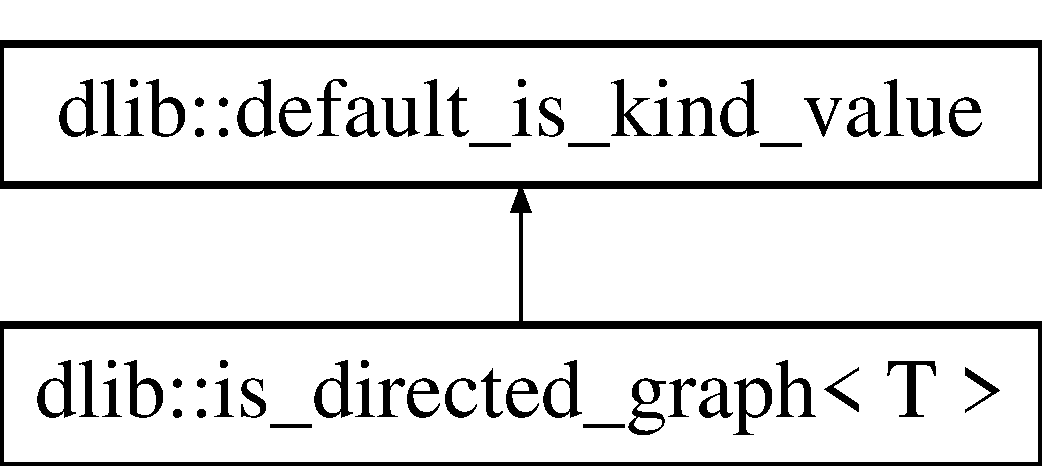
\includegraphics[height=2cm]{structdlib_1_1is__directed__graph}
\end{center}
\end{figure}
\subsubsection*{template$<$typename T$>$ struct dlib::is\_\-directed\_\-graph$<$ T $>$}



The documentation for this struct was generated from the following file:\begin{DoxyCompactItemize}
\item 
source/dlib/is\_\-kind.h\end{DoxyCompactItemize}

\hypertarget{structdlib_1_1is__graph}{
\section{dlib::is\_\-graph$<$ T $>$ Struct Template Reference}
\label{structdlib_1_1is__graph}\index{dlib::is\_\-graph@{dlib::is\_\-graph}}
}
Inheritance diagram for dlib::is\_\-graph$<$ T $>$::\begin{figure}[H]
\begin{center}
\leavevmode
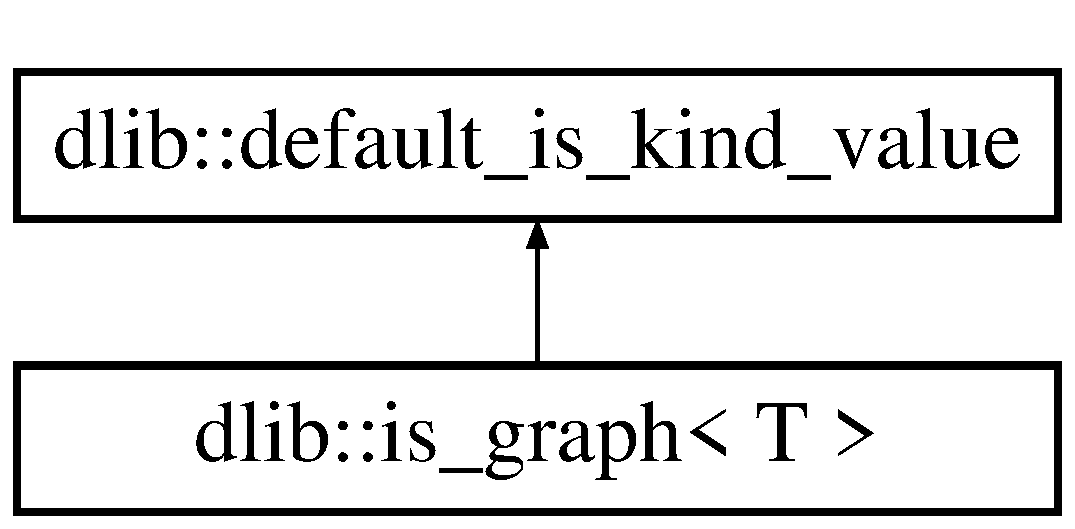
\includegraphics[height=2cm]{structdlib_1_1is__graph}
\end{center}
\end{figure}
\subsubsection*{template$<$typename T$>$ struct dlib::is\_\-graph$<$ T $>$}



The documentation for this struct was generated from the following file:\begin{DoxyCompactItemize}
\item 
source/dlib/is\_\-kind.h\end{DoxyCompactItemize}

\hypertarget{structdlib_1_1is__matrix}{
\section{dlib::is\_\-matrix$<$ T, helper $>$ Struct Template Reference}
\label{structdlib_1_1is__matrix}\index{dlib::is\_\-matrix@{dlib::is\_\-matrix}}
}
Inheritance diagram for dlib::is\_\-matrix$<$ T, helper $>$::\begin{figure}[H]
\begin{center}
\leavevmode
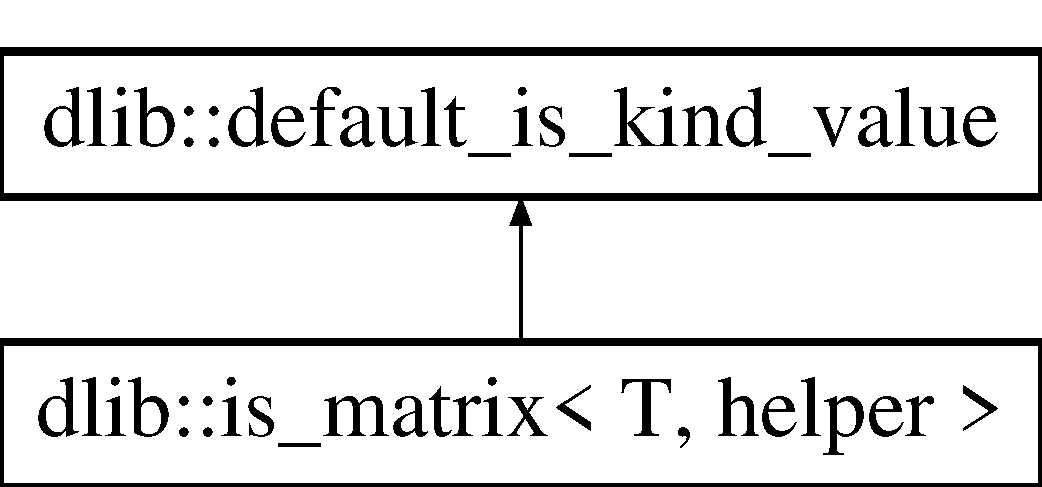
\includegraphics[height=2cm]{structdlib_1_1is__matrix}
\end{center}
\end{figure}
\subsection*{Public Member Functions}
\begin{DoxyCompactItemize}
\item 
\hyperlink{structdlib_1_1is__matrix_abb2a105e957c1e12a8524f7c8d200cc4}{ASSERT\_\-ARE\_\-SAME\_\-TYPE} (helper, void)
\end{DoxyCompactItemize}
\subsubsection*{template$<$typename T, typename helper = void$>$ struct dlib::is\_\-matrix$<$ T, helper $>$}



\subsection{Member Function Documentation}
\hypertarget{structdlib_1_1is__matrix_abb2a105e957c1e12a8524f7c8d200cc4}{
\index{dlib::is\_\-matrix@{dlib::is\_\-matrix}!ASSERT\_\-ARE\_\-SAME\_\-TYPE@{ASSERT\_\-ARE\_\-SAME\_\-TYPE}}
\index{ASSERT\_\-ARE\_\-SAME\_\-TYPE@{ASSERT\_\-ARE\_\-SAME\_\-TYPE}!dlib::is_matrix@{dlib::is\_\-matrix}}
\subsubsection[{ASSERT\_\-ARE\_\-SAME\_\-TYPE}]{\setlength{\rightskip}{0pt plus 5cm}template$<$typename T , typename helper  = void$>$ {\bf dlib::is\_\-matrix}$<$ T, helper $>$::ASSERT\_\-ARE\_\-SAME\_\-TYPE (helper, \/  void)}}
\label{structdlib_1_1is__matrix_abb2a105e957c1e12a8524f7c8d200cc4}

\begin{DoxyItemize}
\item if (T is some kind of matrix expression from the matrix/matrix\_\-abstract.h component) then
\begin{DoxyItemize}
\item is\_\-matrix$<$T$>$::value == true
\end{DoxyItemize}
\item else
\begin{DoxyItemize}
\item is\_\-matrix$<$T$>$::value == false ! 
\end{DoxyItemize}
\end{DoxyItemize}

The documentation for this struct was generated from the following file:\begin{DoxyCompactItemize}
\item 
source/dlib/is\_\-kind.h\end{DoxyCompactItemize}

\hypertarget{classdlib_1_1is__pointer__type}{
\section{dlib::is\_\-pointer\_\-type$<$ T $>$ Class Template Reference}
\label{classdlib_1_1is__pointer__type}\index{dlib::is\_\-pointer\_\-type@{dlib::is\_\-pointer\_\-type}}
}


{\ttfamily \#include $<$algs.h$>$}\subsection*{Public Types}
\begin{DoxyCompactItemize}
\item 
enum \{ {\bfseries value} =  false
 \}
\end{DoxyCompactItemize}


\subsection{Detailed Description}
\subsubsection*{template$<$typename T$>$ class dlib::is\_\-pointer\_\-type$<$ T $>$}

A \hyperlink{classdlib_1_1is__pointer__type}{is\_\-pointer\_\-type}

This is a template where is\_\-pointer\_\-type$<$T$>$::value == true when T is a pointer type ane false otherwise. ! 

The documentation for this class was generated from the following file:\begin{DoxyCompactItemize}
\item 
source/dlib/algs.h\end{DoxyCompactItemize}

\hypertarget{classdlib_1_1is__pointer__type_3_01T_01_5_01_4}{
\section{dlib::is\_\-pointer\_\-type$<$ T $\ast$ $>$ Class Template Reference}
\label{classdlib_1_1is__pointer__type_3_01T_01_5_01_4}\index{dlib::is\_\-pointer\_\-type$<$ T $\ast$ $>$@{dlib::is\_\-pointer\_\-type$<$ T $\ast$ $>$}}
}
\subsection*{Public Types}
\begin{DoxyCompactItemize}
\item 
enum \{ {\bfseries value} =  true
 \}
\end{DoxyCompactItemize}
\subsubsection*{template$<$typename T$>$ class dlib::is\_\-pointer\_\-type$<$ T $\ast$ $>$}



The documentation for this class was generated from the following file:\begin{DoxyCompactItemize}
\item 
source/dlib/algs.h\end{DoxyCompactItemize}

\hypertarget{structdlib_1_1is__rand}{
\section{dlib::is\_\-rand$<$ T $>$ Struct Template Reference}
\label{structdlib_1_1is__rand}\index{dlib::is\_\-rand@{dlib::is\_\-rand}}
}
Inheritance diagram for dlib::is\_\-rand$<$ T $>$::\begin{figure}[H]
\begin{center}
\leavevmode
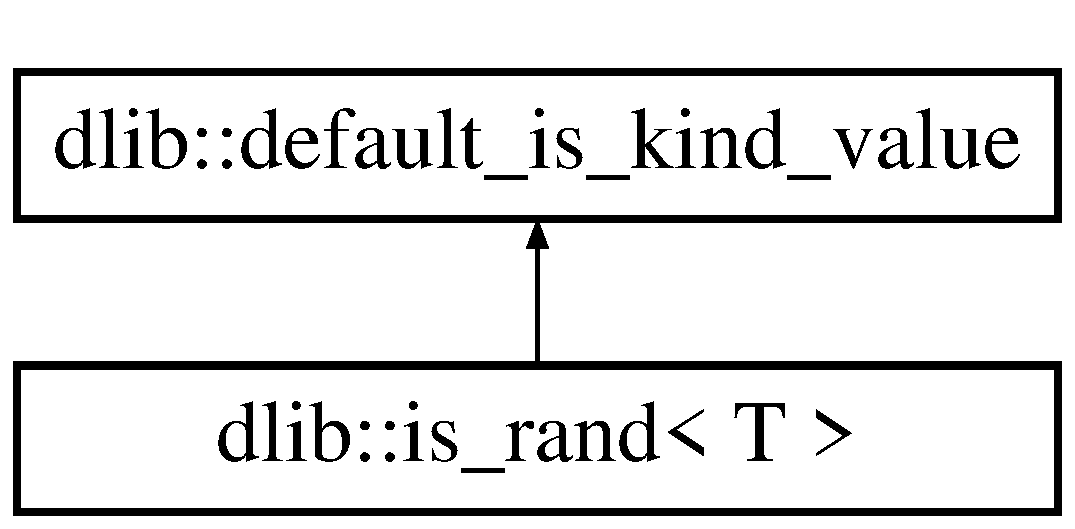
\includegraphics[height=2cm]{structdlib_1_1is__rand}
\end{center}
\end{figure}
\subsubsection*{template$<$typename T$>$ struct dlib::is\_\-rand$<$ T $>$}



The documentation for this struct was generated from the following file:\begin{DoxyCompactItemize}
\item 
source/dlib/is\_\-kind.h\end{DoxyCompactItemize}

\hypertarget{classdlib_1_1is__same__type}{
\section{dlib::is\_\-same\_\-type$<$ T, U $>$ Class Template Reference}
\label{classdlib_1_1is__same__type}\index{dlib::is\_\-same\_\-type@{dlib::is\_\-same\_\-type}}
}


{\ttfamily \#include $<$algs.h$>$}\subsection*{Public Types}
\begin{DoxyCompactItemize}
\item 
enum \{ {\bfseries value} =  false
 \}
\end{DoxyCompactItemize}


\subsection{Detailed Description}
\subsubsection*{template$<$typename T, typename U$>$ class dlib::is\_\-same\_\-type$<$ T, U $>$}

A \hyperlink{classdlib_1_1is__same__type}{is\_\-same\_\-type}

This is a template where is\_\-same\_\-type$<$T,U$>$::value == true when T and U are the same type and false otherwise. ! 

The documentation for this class was generated from the following file:\begin{DoxyCompactItemize}
\item 
source/dlib/algs.h\end{DoxyCompactItemize}

\hypertarget{classdlib_1_1is__same__type_3_01T_00_01T_01_4}{
\section{dlib::is\_\-same\_\-type$<$ T, T $>$ Class Template Reference}
\label{classdlib_1_1is__same__type_3_01T_00_01T_01_4}\index{dlib::is\_\-same\_\-type$<$ T, T $>$@{dlib::is\_\-same\_\-type$<$ T, T $>$}}
}
\subsection*{Public Types}
\begin{DoxyCompactItemize}
\item 
enum \{ {\bfseries value} =  true
 \}
\end{DoxyCompactItemize}
\subsubsection*{template$<$typename T$>$ class dlib::is\_\-same\_\-type$<$ T, T $>$}



The documentation for this class was generated from the following file:\begin{DoxyCompactItemize}
\item 
source/dlib/algs.h\end{DoxyCompactItemize}

\hypertarget{structdlib_1_1is__signed__type}{
\section{dlib::is\_\-signed\_\-type$<$ T $>$ Struct Template Reference}
\label{structdlib_1_1is__signed__type}\index{dlib::is\_\-signed\_\-type@{dlib::is\_\-signed\_\-type}}
}


{\ttfamily \#include $<$algs.h$>$}\subsection*{Static Public Attributes}
\begin{DoxyCompactItemize}
\item 
\hypertarget{structdlib_1_1is__signed__type_ac0288d0dddbeb5c11a612739b7ae952e}{
static const bool {\bfseries value} = !\hyperlink{structdlib_1_1is__unsigned__type}{is\_\-unsigned\_\-type}$<$T$>$::value}
\label{structdlib_1_1is__signed__type_ac0288d0dddbeb5c11a612739b7ae952e}

\end{DoxyCompactItemize}


\subsection{Detailed Description}
\subsubsection*{template$<$typename T$>$ struct dlib::is\_\-signed\_\-type$<$ T $>$}

A \hyperlink{structdlib_1_1is__signed__type}{is\_\-signed\_\-type}

This is a template where is\_\-signed\_\-type$<$T$>$::value == true when T is a signed integral type and false when T is an unsigned integral type. ! 

The documentation for this struct was generated from the following file:\begin{DoxyCompactItemize}
\item 
source/dlib/algs.h\end{DoxyCompactItemize}

\hypertarget{structdlib_1_1is__std__vector}{
\section{dlib::is\_\-std\_\-vector$<$ T $>$ Struct Template Reference}
\label{structdlib_1_1is__std__vector}\index{dlib::is\_\-std\_\-vector@{dlib::is\_\-std\_\-vector}}
}
Inheritance diagram for dlib::is\_\-std\_\-vector$<$ T $>$::\begin{figure}[H]
\begin{center}
\leavevmode
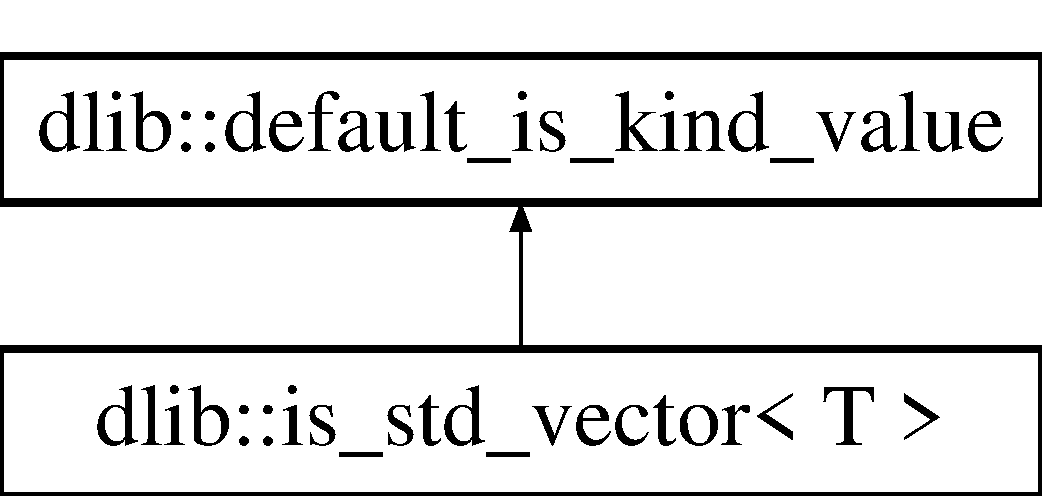
\includegraphics[height=2cm]{structdlib_1_1is__std__vector}
\end{center}
\end{figure}
\subsubsection*{template$<$typename T$>$ struct dlib::is\_\-std\_\-vector$<$ T $>$}



The documentation for this struct was generated from the following file:\begin{DoxyCompactItemize}
\item 
source/dlib/is\_\-kind.h\end{DoxyCompactItemize}

\hypertarget{structdlib_1_1is__std__vector_3_01const_01T_01_6_01_4}{
\section{dlib::is\_\-std\_\-vector$<$ const T \& $>$ Struct Template Reference}
\label{structdlib_1_1is__std__vector_3_01const_01T_01_6_01_4}\index{dlib::is\_\-std\_\-vector$<$ const T \& $>$@{dlib::is\_\-std\_\-vector$<$ const T \& $>$}}
}
\subsection*{Static Public Attributes}
\begin{DoxyCompactItemize}
\item 
\hypertarget{structdlib_1_1is__std__vector_3_01const_01T_01_6_01_4_a2182542008a9b43fd7705f484d226695}{
static const bool {\bfseries value} = \hyperlink{structdlib_1_1is__std__vector}{is\_\-std\_\-vector}$<$T$>$::value}
\label{structdlib_1_1is__std__vector_3_01const_01T_01_6_01_4_a2182542008a9b43fd7705f484d226695}

\end{DoxyCompactItemize}
\subsubsection*{template$<$typename T$>$ struct dlib::is\_\-std\_\-vector$<$ const T \& $>$}



The documentation for this struct was generated from the following file:\begin{DoxyCompactItemize}
\item 
source/dlib/is\_\-kind.h\end{DoxyCompactItemize}

\hypertarget{structdlib_1_1is__std__vector_3_01const_01T_01_4}{
\section{dlib::is\_\-std\_\-vector$<$ const T $>$ Struct Template Reference}
\label{structdlib_1_1is__std__vector_3_01const_01T_01_4}\index{dlib::is\_\-std\_\-vector$<$ const T $>$@{dlib::is\_\-std\_\-vector$<$ const T $>$}}
}
\subsection*{Static Public Attributes}
\begin{DoxyCompactItemize}
\item 
\hypertarget{structdlib_1_1is__std__vector_3_01const_01T_01_4_a0d5baed76a7ae3203b0bc4a0440158de}{
static const bool {\bfseries value} = \hyperlink{structdlib_1_1is__std__vector}{is\_\-std\_\-vector}$<$T$>$::value}
\label{structdlib_1_1is__std__vector_3_01const_01T_01_4_a0d5baed76a7ae3203b0bc4a0440158de}

\end{DoxyCompactItemize}
\subsubsection*{template$<$typename T$>$ struct dlib::is\_\-std\_\-vector$<$ const T $>$}



The documentation for this struct was generated from the following file:\begin{DoxyCompactItemize}
\item 
source/dlib/is\_\-kind.h\end{DoxyCompactItemize}

\hypertarget{structdlib_1_1is__std__vector_3_01std_1_1vector_3_01T_00_01alloc_01_4_01_4}{
\section{dlib::is\_\-std\_\-vector$<$ std::vector$<$ T, alloc $>$ $>$ Struct Template Reference}
\label{structdlib_1_1is__std__vector_3_01std_1_1vector_3_01T_00_01alloc_01_4_01_4}\index{dlib::is\_\-std\_\-vector$<$ std::vector$<$ T, alloc $>$ $>$@{dlib::is\_\-std\_\-vector$<$ std::vector$<$ T, alloc $>$ $>$}}
}
\subsection*{Static Public Attributes}
\begin{DoxyCompactItemize}
\item 
\hypertarget{structdlib_1_1is__std__vector_3_01std_1_1vector_3_01T_00_01alloc_01_4_01_4_a15a53bfa55e7761ee5193c2389597cdb}{
static const bool {\bfseries value} = true}
\label{structdlib_1_1is__std__vector_3_01std_1_1vector_3_01T_00_01alloc_01_4_01_4_a15a53bfa55e7761ee5193c2389597cdb}

\end{DoxyCompactItemize}
\subsubsection*{template$<$typename T, typename alloc$>$ struct dlib::is\_\-std\_\-vector$<$ std::vector$<$ T, alloc $>$ $>$}



The documentation for this struct was generated from the following file:\begin{DoxyCompactItemize}
\item 
source/dlib/is\_\-kind.h\end{DoxyCompactItemize}

\hypertarget{structdlib_1_1is__std__vector_3_01T_01_6_01_4}{
\section{dlib::is\_\-std\_\-vector$<$ T \& $>$ Struct Template Reference}
\label{structdlib_1_1is__std__vector_3_01T_01_6_01_4}\index{dlib::is\_\-std\_\-vector$<$ T \& $>$@{dlib::is\_\-std\_\-vector$<$ T \& $>$}}
}
\subsection*{Static Public Attributes}
\begin{DoxyCompactItemize}
\item 
\hypertarget{structdlib_1_1is__std__vector_3_01T_01_6_01_4_a4a48b8853174a254bb75f54f77583785}{
static const bool {\bfseries value} = \hyperlink{structdlib_1_1is__std__vector}{is\_\-std\_\-vector}$<$T$>$::value}
\label{structdlib_1_1is__std__vector_3_01T_01_6_01_4_a4a48b8853174a254bb75f54f77583785}

\end{DoxyCompactItemize}
\subsubsection*{template$<$typename T$>$ struct dlib::is\_\-std\_\-vector$<$ T \& $>$}



The documentation for this struct was generated from the following file:\begin{DoxyCompactItemize}
\item 
source/dlib/is\_\-kind.h\end{DoxyCompactItemize}

\hypertarget{structdlib_1_1is__unsigned__type}{
\section{dlib::is\_\-unsigned\_\-type$<$ T $>$ Struct Template Reference}
\label{structdlib_1_1is__unsigned__type}\index{dlib::is\_\-unsigned\_\-type@{dlib::is\_\-unsigned\_\-type}}
}


{\ttfamily \#include $<$algs.h$>$}\subsection*{Static Public Attributes}
\begin{DoxyCompactItemize}
\item 
\hypertarget{structdlib_1_1is__unsigned__type_adcd8ee9c065998d8366549eb636cf58e}{
static const bool {\bfseries value} = static\_\-cast$<$T$>$((static\_\-cast$<$T$>$(0)-\/static\_\-cast$<$T$>$(1))) $>$ 0}
\label{structdlib_1_1is__unsigned__type_adcd8ee9c065998d8366549eb636cf58e}

\end{DoxyCompactItemize}


\subsection{Detailed Description}
\subsubsection*{template$<$typename T$>$ struct dlib::is\_\-unsigned\_\-type$<$ T $>$}

A \hyperlink{structdlib_1_1is__unsigned__type}{is\_\-unsigned\_\-type}

This is a template where is\_\-unsigned\_\-type$<$T$>$::value == true when T is an unsigned integral type and false when T is a signed integral type. ! 

The documentation for this struct was generated from the following file:\begin{DoxyCompactItemize}
\item 
source/dlib/algs.h\end{DoxyCompactItemize}

\hypertarget{classIsometricConversions}{
\section{IsometricConversions Class Reference}
\label{classIsometricConversions}\index{IsometricConversions@{IsometricConversions}}
}
\subsection*{Static Public Member Functions}
\begin{DoxyCompactItemize}
\item 
\hypertarget{classIsometricConversions_a925fb6ecff83501f956092ebd4c237ce}{
static CL\_\-Pointf {\bfseries worldToIsometric} (CL\_\-Pointf)}
\label{classIsometricConversions_a925fb6ecff83501f956092ebd4c237ce}

\item 
\hypertarget{classIsometricConversions_a039c5054ad98fa76218151f39941a3d8}{
static CL\_\-Pointd {\bfseries worldToIsometric} (CL\_\-Pointd)}
\label{classIsometricConversions_a039c5054ad98fa76218151f39941a3d8}

\item 
\hypertarget{classIsometricConversions_a97f4247e5ab8e730432bda5da0be3527}{
static CL\_\-Pointd {\bfseries isometricToWorld} (CL\_\-Pointd)}
\label{classIsometricConversions_a97f4247e5ab8e730432bda5da0be3527}

\end{DoxyCompactItemize}


The documentation for this class was generated from the following files:\begin{DoxyCompactItemize}
\item 
source/game/\hyperlink{IsometricConversions_8h}{IsometricConversions.h}\item 
source/game/\hyperlink{IsometricConversions_8cpp}{IsometricConversions.cpp}\end{DoxyCompactItemize}

\hypertarget{classIsometricGrid}{
\section{IsometricGrid Class Reference}
\label{classIsometricGrid}\index{IsometricGrid@{IsometricGrid}}
}


{\ttfamily \#include $<$IsometricGrid.h$>$}Inheritance diagram for IsometricGrid::\begin{figure}[H]
\begin{center}
\leavevmode
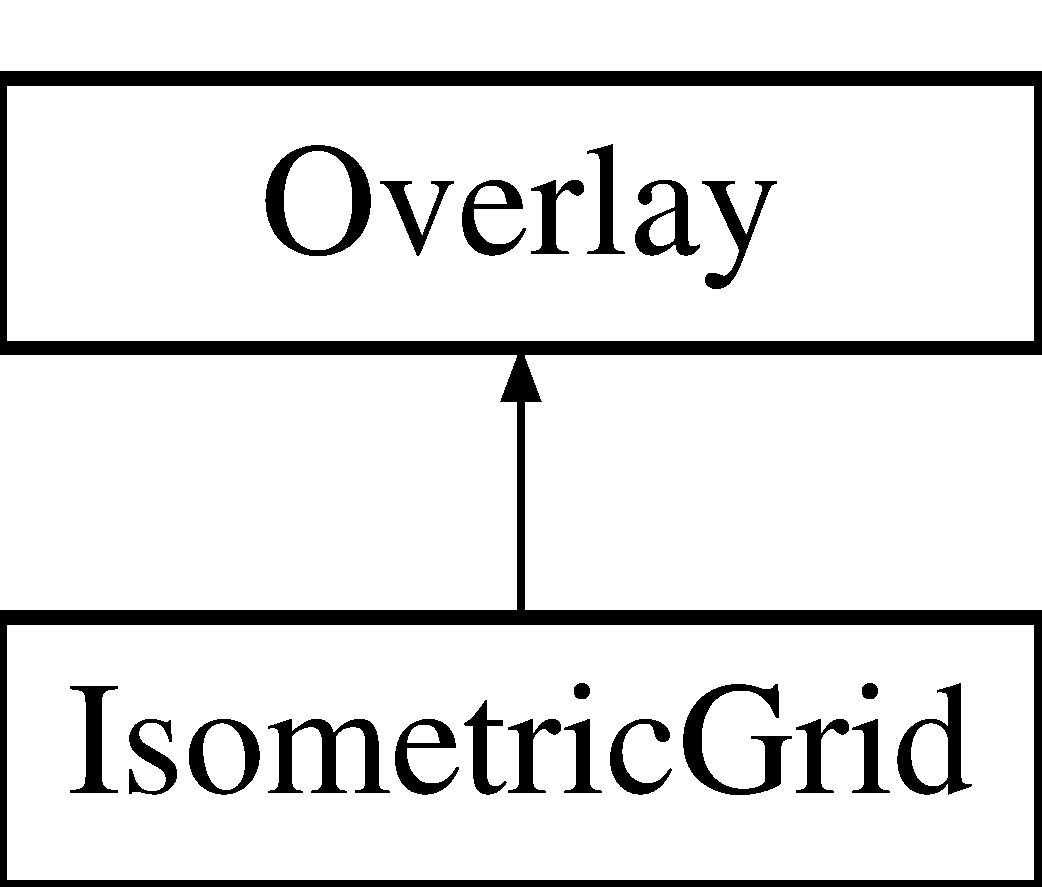
\includegraphics[height=2cm]{classIsometricGrid}
\end{center}
\end{figure}
\subsection*{Public Member Functions}
\begin{DoxyCompactItemize}
\item 
\hypertarget{classIsometricGrid_a4ac39773481a3937b415a71e8e7a29bd}{
{\bfseries IsometricGrid} (\hyperlink{classWorld}{World} $\ast$)}
\label{classIsometricGrid_a4ac39773481a3937b415a71e8e7a29bd}

\item 
\hypertarget{classIsometricGrid_a3138024ea901361f87a47c008fe4f31d}{
void {\bfseries draw} (void)}
\label{classIsometricGrid_a3138024ea901361f87a47c008fe4f31d}

\end{DoxyCompactItemize}


\subsection{Detailed Description}
Constructs a very basic 60x60 isometric grid overlay when calling the draw() function. 

The documentation for this class was generated from the following files:\begin{DoxyCompactItemize}
\item 
IsometricGrid.h\item 
IsometricGrid.cpp\end{DoxyCompactItemize}

\hypertarget{classdlib_1_1joint__probability__table}{
\section{dlib::joint\_\-probability\_\-table Class Reference}
\label{classdlib_1_1joint__probability__table}\index{dlib::joint\_\-probability\_\-table@{dlib::joint\_\-probability\_\-table}}
}
\subsection*{Public Member Functions}
\begin{DoxyCompactItemize}
\item 
\hyperlink{classdlib_1_1joint__probability__table_a68ba392924a2080a56d0246b7b01b7a2}{joint\_\-probability\_\-table} (const \hyperlink{classdlib_1_1joint__probability__table}{joint\_\-probability\_\-table} \&t)
\item 
\hypertarget{classdlib_1_1joint__probability__table_aee768f051adb65237a6312e6b6ba721d}{
\hyperlink{classdlib_1_1joint__probability__table}{joint\_\-probability\_\-table} \& {\bfseries operator=} (const \hyperlink{classdlib_1_1joint__probability__table}{joint\_\-probability\_\-table} \&rhs)}
\label{classdlib_1_1joint__probability__table_aee768f051adb65237a6312e6b6ba721d}

\item 
\hypertarget{classdlib_1_1joint__probability__table_a678d75a7ad42da9aae974547278abc4f}{
void {\bfseries set\_\-probability} (const \hyperlink{classdlib_1_1assignment}{assignment} \&a, double p)}
\label{classdlib_1_1joint__probability__table_a678d75a7ad42da9aae974547278abc4f}

\item 
\hypertarget{classdlib_1_1joint__probability__table_acfd6d1ce03bf921ec68b517ed3274c77}{
bool {\bfseries has\_\-entry\_\-for} (const \hyperlink{classdlib_1_1assignment}{assignment} \&a) const }
\label{classdlib_1_1joint__probability__table_acfd6d1ce03bf921ec68b517ed3274c77}

\item 
\hypertarget{classdlib_1_1joint__probability__table_af9edf3c0a627e056c568d9bab7b0aeaa}{
void {\bfseries add\_\-probability} (const \hyperlink{classdlib_1_1assignment}{assignment} \&a, double p)}
\label{classdlib_1_1joint__probability__table_af9edf3c0a627e056c568d9bab7b0aeaa}

\item 
\hypertarget{classdlib_1_1joint__probability__table_a799394abc1dcfe9e840a56dc53271408}{
double {\bfseries probability} (const \hyperlink{classdlib_1_1assignment}{assignment} \&a) const }
\label{classdlib_1_1joint__probability__table_a799394abc1dcfe9e840a56dc53271408}

\item 
\hypertarget{classdlib_1_1joint__probability__table_a0fdadc3b0d50dfb1750004c5e8eb45a5}{
void {\bfseries clear} ()}
\label{classdlib_1_1joint__probability__table_a0fdadc3b0d50dfb1750004c5e8eb45a5}

\item 
\hypertarget{classdlib_1_1joint__probability__table_a6f89f7c5b1047930740e988a30e70deb}{
unsigned long {\bfseries size} () const }
\label{classdlib_1_1joint__probability__table_a6f89f7c5b1047930740e988a30e70deb}

\item 
\hypertarget{classdlib_1_1joint__probability__table_ae5a43662465634b1eae8c976ffc12684}{
bool {\bfseries move\_\-next} () const }
\label{classdlib_1_1joint__probability__table_ae5a43662465634b1eae8c976ffc12684}

\item 
\hypertarget{classdlib_1_1joint__probability__table_a9767a770bb7e4baf697d7cbf430afa87}{
void {\bfseries reset} () const }
\label{classdlib_1_1joint__probability__table_a9767a770bb7e4baf697d7cbf430afa87}

\item 
\hypertarget{classdlib_1_1joint__probability__table_a0ab414af6311c50e73930d8482dafc87}{
map\_\-pair$<$ \hyperlink{classdlib_1_1assignment}{assignment}, double $>$ \& {\bfseries element} ()}
\label{classdlib_1_1joint__probability__table_a0ab414af6311c50e73930d8482dafc87}

\item 
\hypertarget{classdlib_1_1joint__probability__table_a4fb635d9c175ce8ebc7a4ee7715799dc}{
const map\_\-pair$<$ \hyperlink{classdlib_1_1assignment}{assignment}, double $>$ \& {\bfseries element} () const }
\label{classdlib_1_1joint__probability__table_a4fb635d9c175ce8ebc7a4ee7715799dc}

\item 
\hypertarget{classdlib_1_1joint__probability__table_a431f184917878ad1778e57c9c0ca5ea2}{
bool {\bfseries at\_\-start} () const }
\label{classdlib_1_1joint__probability__table_a431f184917878ad1778e57c9c0ca5ea2}

\item 
\hypertarget{classdlib_1_1joint__probability__table_a7842bab03b20b08947700ac4766544fc}{
bool {\bfseries current\_\-element\_\-valid} () const }
\label{classdlib_1_1joint__probability__table_a7842bab03b20b08947700ac4766544fc}

\item 
\hypertarget{classdlib_1_1joint__probability__table_a1b9d9b5ca2c15171969b7e4fc758f6e6}{
{\footnotesize template$<$typename T $>$ }\\void {\bfseries marginalize} (const T \&vars, \hyperlink{classdlib_1_1joint__probability__table}{joint\_\-probability\_\-table} \&out) const }
\label{classdlib_1_1joint__probability__table_a1b9d9b5ca2c15171969b7e4fc758f6e6}

\item 
\hypertarget{classdlib_1_1joint__probability__table_a1cfe903f47b2bbc69e75b4fa6bfc3b79}{
void {\bfseries marginalize} (const unsigned long var, \hyperlink{classdlib_1_1joint__probability__table}{joint\_\-probability\_\-table} \&out) const }
\label{classdlib_1_1joint__probability__table_a1cfe903f47b2bbc69e75b4fa6bfc3b79}

\item 
\hypertarget{classdlib_1_1joint__probability__table_a2886ef7c11d08c6b294dd34348ae81ca}{
void {\bfseries normalize} ()}
\label{classdlib_1_1joint__probability__table_a2886ef7c11d08c6b294dd34348ae81ca}

\item 
\hypertarget{classdlib_1_1joint__probability__table_a971c4513f167bf91df70836e579ebed6}{
void {\bfseries swap} (\hyperlink{classdlib_1_1joint__probability__table}{joint\_\-probability\_\-table} \&item)}
\label{classdlib_1_1joint__probability__table_a971c4513f167bf91df70836e579ebed6}

\end{DoxyCompactItemize}
\subsection*{Friends}
\begin{DoxyCompactItemize}
\item 
\hypertarget{classdlib_1_1joint__probability__table_ac8164cee0a2afc188db58cf8b9f956ce}{
void {\bfseries serialize} (const \hyperlink{classdlib_1_1joint__probability__table}{joint\_\-probability\_\-table} \&item, std::ostream \&out)}
\label{classdlib_1_1joint__probability__table_ac8164cee0a2afc188db58cf8b9f956ce}

\item 
\hypertarget{classdlib_1_1joint__probability__table_a8a45c8c2ae3fe15192383713af6ed400}{
void {\bfseries deserialize} (\hyperlink{classdlib_1_1joint__probability__table}{joint\_\-probability\_\-table} \&item, std::istream \&in)}
\label{classdlib_1_1joint__probability__table_a8a45c8c2ae3fe15192383713af6ed400}

\end{DoxyCompactItemize}


\subsection{Constructor \& Destructor Documentation}
\hypertarget{classdlib_1_1joint__probability__table_a68ba392924a2080a56d0246b7b01b7a2}{
\index{dlib::joint\_\-probability\_\-table@{dlib::joint\_\-probability\_\-table}!joint\_\-probability\_\-table@{joint\_\-probability\_\-table}}
\index{joint\_\-probability\_\-table@{joint\_\-probability\_\-table}!dlib::joint_probability_table@{dlib::joint\_\-probability\_\-table}}
\subsubsection[{joint\_\-probability\_\-table}]{\setlength{\rightskip}{0pt plus 5cm}dlib::joint\_\-probability\_\-table::joint\_\-probability\_\-table (const {\bf joint\_\-probability\_\-table} \& {\em t})\hspace{0.3cm}{\ttfamily  \mbox{[}inline\mbox{]}}}}
\label{classdlib_1_1joint__probability__table_a68ba392924a2080a56d0246b7b01b7a2}
INITIAL VALUE
\begin{DoxyItemize}
\item table.size() == 0
\end{DoxyItemize}

CONVENTION
\begin{DoxyItemize}
\item size() == table.size()
\item probability(a) == table\mbox{[}a\mbox{]} ! 
\end{DoxyItemize}

The documentation for this class was generated from the following file:\begin{DoxyCompactItemize}
\item 
source/dlib/bayes\_\-utils/bayes\_\-utils.h\end{DoxyCompactItemize}

\hypertarget{structboost_1_1lazy__disable__if}{
\section{boost::lazy\_\-disable\_\-if$<$ Cond, T $>$ Struct Template Reference}
\label{structboost_1_1lazy__disable__if}\index{boost::lazy\_\-disable\_\-if@{boost::lazy\_\-disable\_\-if}}
}
Inheritance diagram for boost::lazy\_\-disable\_\-if$<$ Cond, T $>$::\begin{figure}[H]
\begin{center}
\leavevmode
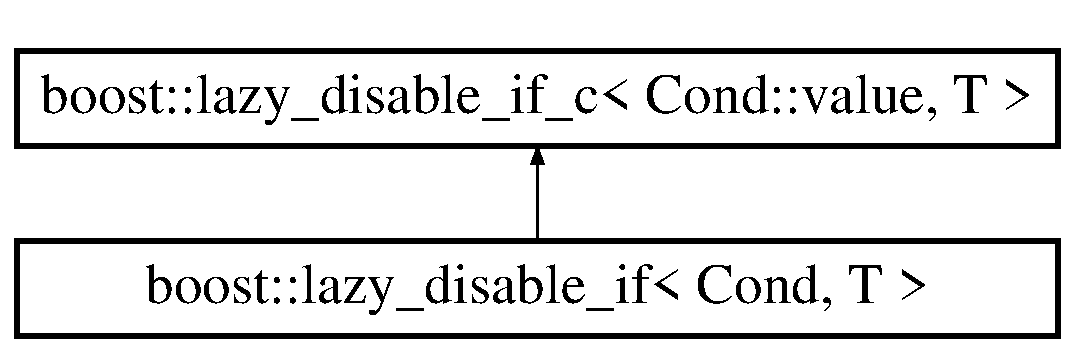
\includegraphics[height=2cm]{structboost_1_1lazy__disable__if}
\end{center}
\end{figure}
\subsubsection*{template$<$class Cond, class T$>$ struct boost::lazy\_\-disable\_\-if$<$ Cond, T $>$}



The documentation for this struct was generated from the following file:\begin{DoxyCompactItemize}
\item 
source/dlib/enable\_\-if.h\end{DoxyCompactItemize}

\hypertarget{structboost_1_1lazy__disable__if__c}{
\section{boost::lazy\_\-disable\_\-if\_\-c$<$ B, T $>$ Struct Template Reference}
\label{structboost_1_1lazy__disable__if__c}\index{boost::lazy\_\-disable\_\-if\_\-c@{boost::lazy\_\-disable\_\-if\_\-c}}
}
\subsection*{Public Types}
\begin{DoxyCompactItemize}
\item 
\hypertarget{structboost_1_1lazy__disable__if__c_ac7a275a383b5bae04cf23cfe7948a68a}{
typedef T::type {\bfseries type}}
\label{structboost_1_1lazy__disable__if__c_ac7a275a383b5bae04cf23cfe7948a68a}

\end{DoxyCompactItemize}
\subsubsection*{template$<$bool B, class T$>$ struct boost::lazy\_\-disable\_\-if\_\-c$<$ B, T $>$}



The documentation for this struct was generated from the following file:\begin{DoxyCompactItemize}
\item 
source/dlib/enable\_\-if.h\end{DoxyCompactItemize}

\hypertarget{structboost_1_1lazy__disable__if__c_3_01true_00_01T_01_4}{
\section{boost::lazy\_\-disable\_\-if\_\-c$<$ true, T $>$ Struct Template Reference}
\label{structboost_1_1lazy__disable__if__c_3_01true_00_01T_01_4}\index{boost::lazy\_\-disable\_\-if\_\-c$<$ true, T $>$@{boost::lazy\_\-disable\_\-if\_\-c$<$ true, T $>$}}
}
\subsubsection*{template$<$class T$>$ struct boost::lazy\_\-disable\_\-if\_\-c$<$ true, T $>$}



The documentation for this struct was generated from the following file:\begin{DoxyCompactItemize}
\item 
source/dlib/enable\_\-if.h\end{DoxyCompactItemize}

\hypertarget{structboost_1_1lazy__enable__if}{
\section{boost::lazy\_\-enable\_\-if$<$ Cond, T $>$ Struct Template Reference}
\label{structboost_1_1lazy__enable__if}\index{boost::lazy\_\-enable\_\-if@{boost::lazy\_\-enable\_\-if}}
}
Inheritance diagram for boost::lazy\_\-enable\_\-if$<$ Cond, T $>$::\begin{figure}[H]
\begin{center}
\leavevmode
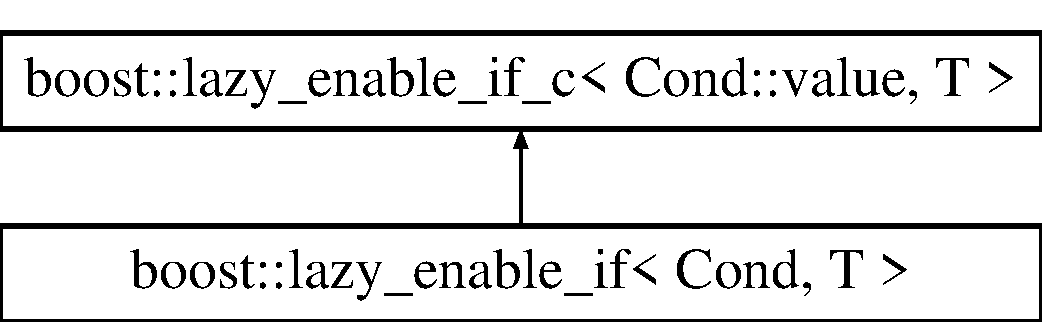
\includegraphics[height=2cm]{structboost_1_1lazy__enable__if}
\end{center}
\end{figure}
\subsubsection*{template$<$class Cond, class T$>$ struct boost::lazy\_\-enable\_\-if$<$ Cond, T $>$}



The documentation for this struct was generated from the following file:\begin{DoxyCompactItemize}
\item 
source/dlib/enable\_\-if.h\end{DoxyCompactItemize}

\hypertarget{structboost_1_1lazy__enable__if__c}{
\section{boost::lazy\_\-enable\_\-if\_\-c$<$ B, T $>$ Struct Template Reference}
\label{structboost_1_1lazy__enable__if__c}\index{boost::lazy\_\-enable\_\-if\_\-c@{boost::lazy\_\-enable\_\-if\_\-c}}
}
\subsection*{Public Types}
\begin{DoxyCompactItemize}
\item 
\hypertarget{structboost_1_1lazy__enable__if__c_af11bb72718b0a05956dea253d0517d7a}{
typedef T::type {\bfseries type}}
\label{structboost_1_1lazy__enable__if__c_af11bb72718b0a05956dea253d0517d7a}

\end{DoxyCompactItemize}
\subsubsection*{template$<$bool B, class T$>$ struct boost::lazy\_\-enable\_\-if\_\-c$<$ B, T $>$}



The documentation for this struct was generated from the following file:\begin{DoxyCompactItemize}
\item 
source/dlib/enable\_\-if.h\end{DoxyCompactItemize}

\hypertarget{structboost_1_1lazy__enable__if__c_3_01false_00_01T_01_4}{
\section{boost::lazy\_\-enable\_\-if\_\-c$<$ false, T $>$ Struct Template Reference}
\label{structboost_1_1lazy__enable__if__c_3_01false_00_01T_01_4}\index{boost::lazy\_\-enable\_\-if\_\-c$<$ false, T $>$@{boost::lazy\_\-enable\_\-if\_\-c$<$ false, T $>$}}
}
\subsubsection*{template$<$class T$>$ struct boost::lazy\_\-enable\_\-if\_\-c$<$ false, T $>$}



The documentation for this struct was generated from the following file:\begin{DoxyCompactItemize}
\item 
source/dlib/enable\_\-if.h\end{DoxyCompactItemize}

\hypertarget{classdlib_1_1linker}{
\section{dlib::linker Class Reference}
\label{classdlib_1_1linker}\index{dlib::linker@{dlib::linker}}
}
\subsection*{Public Types}
\begin{DoxyCompactItemize}
\item 
\hypertarget{classdlib_1_1linker_a17f6056c713df703495ebe48865ad003}{
typedef linker\_\-kernel\_\-1 {\bfseries kernel\_\-1a}}
\label{classdlib_1_1linker_a17f6056c713df703495ebe48865ad003}

\item 
\hypertarget{classdlib_1_1linker_a5c2c8f001f8a1c5f78d05122e34b9245}{
typedef linker\_\-kernel\_\-c$<$ kernel\_\-1a $>$ {\bfseries kernel\_\-1a\_\-c}}
\label{classdlib_1_1linker_a5c2c8f001f8a1c5f78d05122e34b9245}

\end{DoxyCompactItemize}


The documentation for this class was generated from the following file:\begin{DoxyCompactItemize}
\item 
source/dlib/linker.h\end{DoxyCompactItemize}

\hypertarget{classdlib_1_1lz77__buffer}{
\section{dlib::lz77\_\-buffer Class Reference}
\label{classdlib_1_1lz77__buffer}\index{dlib::lz77\_\-buffer@{dlib::lz77\_\-buffer}}
}
\subsection*{Public Types}
\begin{DoxyCompactItemize}
\item 
\hypertarget{classdlib_1_1lz77__buffer_a94e824c632d26b8718c1ef66e068bdbd}{
typedef lz77\_\-buffer\_\-kernel\_\-1$<$ sb1 $>$ {\bfseries kernel\_\-1a}}
\label{classdlib_1_1lz77__buffer_a94e824c632d26b8718c1ef66e068bdbd}

\item 
\hypertarget{classdlib_1_1lz77__buffer_a7408f05b96e717d6d76e56188d96dbfa}{
typedef lz77\_\-buffer\_\-kernel\_\-c$<$ kernel\_\-1a $>$ {\bfseries kernel\_\-1a\_\-c}}
\label{classdlib_1_1lz77__buffer_a7408f05b96e717d6d76e56188d96dbfa}

\item 
\hypertarget{classdlib_1_1lz77__buffer_a18b691dec9033825ac02f54d339f78fc}{
typedef lz77\_\-buffer\_\-kernel\_\-2$<$ sb1 $>$ {\bfseries kernel\_\-2a}}
\label{classdlib_1_1lz77__buffer_a18b691dec9033825ac02f54d339f78fc}

\item 
\hypertarget{classdlib_1_1lz77__buffer_a685ead13dfdc17c201fbf8d4e4fb1fbf}{
typedef lz77\_\-buffer\_\-kernel\_\-c$<$ kernel\_\-2a $>$ {\bfseries kernel\_\-2a\_\-c}}
\label{classdlib_1_1lz77__buffer_a685ead13dfdc17c201fbf8d4e4fb1fbf}

\end{DoxyCompactItemize}


The documentation for this class was generated from the following file:\begin{DoxyCompactItemize}
\item 
source/dlib/lz77\_\-buffer.h\end{DoxyCompactItemize}

\hypertarget{classdlib_1_1lzp__buffer}{
\section{dlib::lzp\_\-buffer Class Reference}
\label{classdlib_1_1lzp__buffer}\index{dlib::lzp\_\-buffer@{dlib::lzp\_\-buffer}}
}
\subsection*{Public Types}
\begin{DoxyCompactItemize}
\item 
\hypertarget{classdlib_1_1lzp__buffer_a9b4ed39994855ad0a2fb63fa140a0123}{
typedef lzp\_\-buffer\_\-kernel\_\-1$<$ sb1 $>$ {\bfseries kernel\_\-1a}}
\label{classdlib_1_1lzp__buffer_a9b4ed39994855ad0a2fb63fa140a0123}

\item 
\hypertarget{classdlib_1_1lzp__buffer_a2b831404963c2289b6c6b831b8737ee2}{
typedef lzp\_\-buffer\_\-kernel\_\-c$<$ kernel\_\-1a $>$ {\bfseries kernel\_\-1a\_\-c}}
\label{classdlib_1_1lzp__buffer_a2b831404963c2289b6c6b831b8737ee2}

\item 
\hypertarget{classdlib_1_1lzp__buffer_ab714f89153a27a3ab960ece2d885835b}{
typedef lzp\_\-buffer\_\-kernel\_\-2$<$ sb1 $>$ {\bfseries kernel\_\-2a}}
\label{classdlib_1_1lzp__buffer_ab714f89153a27a3ab960ece2d885835b}

\item 
\hypertarget{classdlib_1_1lzp__buffer_a66368910a9a3a0c739ba877af44f12f4}{
typedef lzp\_\-buffer\_\-kernel\_\-c$<$ kernel\_\-2a $>$ {\bfseries kernel\_\-2a\_\-c}}
\label{classdlib_1_1lzp__buffer_a66368910a9a3a0c739ba877af44f12f4}

\end{DoxyCompactItemize}


The documentation for this class was generated from the following file:\begin{DoxyCompactItemize}
\item 
source/dlib/lzp\_\-buffer.h\end{DoxyCompactItemize}

\hypertarget{classMainMenu}{
\section{MainMenu Class Reference}
\label{classMainMenu}\index{MainMenu@{MainMenu}}
}
Inheritance diagram for MainMenu::\begin{figure}[H]
\begin{center}
\leavevmode
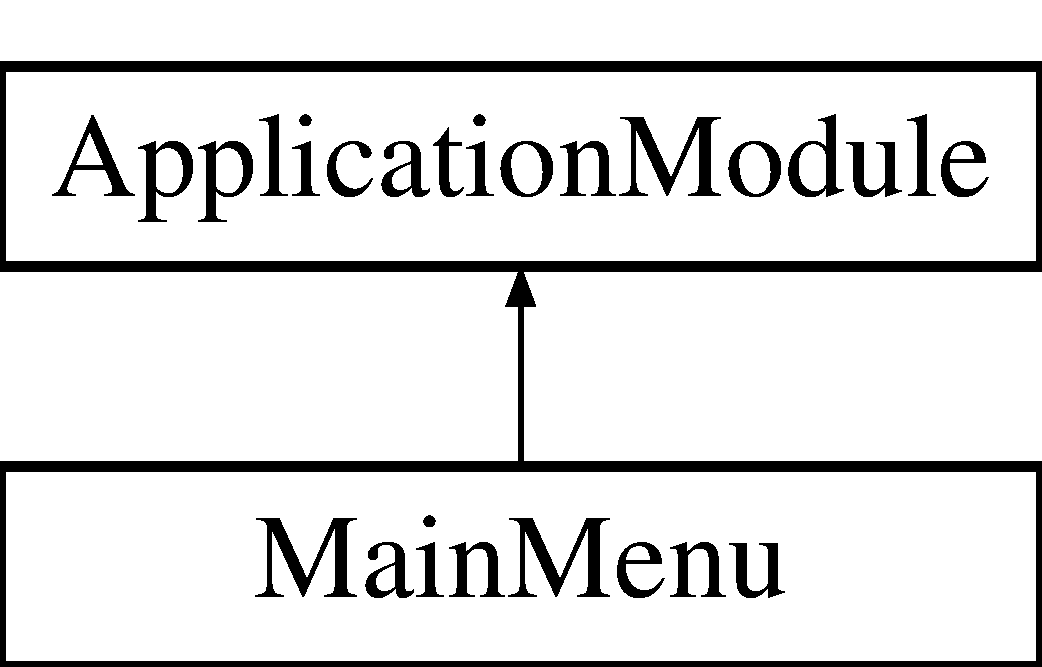
\includegraphics[height=2cm]{classMainMenu}
\end{center}
\end{figure}
\subsection*{Public Member Functions}
\begin{DoxyCompactItemize}
\item 
\hypertarget{classMainMenu_a4f8cb7bce56b9c1053ad0257fa8bec3a}{
{\bfseries MainMenu} (CL\_\-DisplayWindow \&)}
\label{classMainMenu_a4f8cb7bce56b9c1053ad0257fa8bec3a}

\end{DoxyCompactItemize}


The documentation for this class was generated from the following files:\begin{DoxyCompactItemize}
\item 
source/main\_\-menu/\hyperlink{MainMenu_8h}{MainMenu.h}\item 
source/main\_\-menu/\hyperlink{MainMenu_8cpp}{MainMenu.cpp}\end{DoxyCompactItemize}

\hypertarget{classdlib_1_1map}{
\section{dlib::map$<$ domain, range, mem\_\-manager, compare $>$ Class Template Reference}
\label{classdlib_1_1map}\index{dlib::map@{dlib::map}}
}
\subsection*{Public Types}
\begin{DoxyCompactItemize}
\item 
\hypertarget{classdlib_1_1map_aca36b37bfe73286a57138fd644968555}{
typedef map\_\-kernel\_\-1$<$ domain, range, binary\_\-search\_\-tree\_\-1, mem\_\-manager $>$ {\bfseries kernel\_\-1a}}
\label{classdlib_1_1map_aca36b37bfe73286a57138fd644968555}

\item 
\hypertarget{classdlib_1_1map_ab24906726cac87d7a5499a7c6bf1595c}{
typedef map\_\-kernel\_\-c$<$ kernel\_\-1a $>$ {\bfseries kernel\_\-1a\_\-c}}
\label{classdlib_1_1map_ab24906726cac87d7a5499a7c6bf1595c}

\item 
\hypertarget{classdlib_1_1map_ae3e994e8e991bf4899ebad0e264ee5f5}{
typedef map\_\-kernel\_\-1$<$ domain, range, binary\_\-search\_\-tree\_\-2, mem\_\-manager $>$ {\bfseries kernel\_\-1b}}
\label{classdlib_1_1map_ae3e994e8e991bf4899ebad0e264ee5f5}

\item 
\hypertarget{classdlib_1_1map_a9121fd5c57bc2ae6b9acbbb74902087c}{
typedef map\_\-kernel\_\-c$<$ kernel\_\-1b $>$ {\bfseries kernel\_\-1b\_\-c}}
\label{classdlib_1_1map_a9121fd5c57bc2ae6b9acbbb74902087c}

\end{DoxyCompactItemize}
\subsubsection*{template$<$typename domain, typename range, typename mem\_\-manager = memory\_\-manager$<$char$>$::kernel\_\-1a, typename compare = std::less$<$domain$>$$>$ class dlib::map$<$ domain, range, mem\_\-manager, compare $>$}



The documentation for this class was generated from the following file:\begin{DoxyCompactItemize}
\item 
source/dlib/map.h\end{DoxyCompactItemize}

\hypertarget{uniondlib_1_1mem__block}{
\section{dlib::mem\_\-block Union Reference}
\label{uniondlib_1_1mem__block}\index{dlib::mem\_\-block@{dlib::mem\_\-block}}
}
\subsection*{Public Attributes}
\begin{DoxyCompactItemize}
\item 
\hypertarget{uniondlib_1_1mem__block_ae2c6ec8e273befd40944ac4036f1a281}{
void $\ast$ {\bfseries void\_\-ptr}}
\label{uniondlib_1_1mem__block_ae2c6ec8e273befd40944ac4036f1a281}

\item 
\hypertarget{uniondlib_1_1mem__block_ac4e8c1621e9ce339c5928acc6365a9ac}{
int {\bfseries integer}}
\label{uniondlib_1_1mem__block_ac4e8c1621e9ce339c5928acc6365a9ac}

\item 
\hypertarget{uniondlib_1_1mem__block_a2b7d154e09def1e07080f3e264ce8ea6}{
\begin{tabbing}
xx\=xx\=xx\=xx\=xx\=xx\=xx\=xx\=xx\=\kill
struct \{\\
\>void(stack\_based\_memory\_block::$\ast$ {\bfseries callback} )()\\
\>stack\_based\_memory\_block $\ast$ {\bfseries o}\\
\} {\bfseries stuff}}
\label{uniondlib_1_1mem__block_a2b7d154e09def1e07080f3e264ce8ea6}
\\

\end{tabbing}\item 
\hypertarget{uniondlib_1_1mem__block_a447d566f18b5ddbc70eb2bf2da728dfa}{
long double {\bfseries more\_\-stuff}}
\label{uniondlib_1_1mem__block_a447d566f18b5ddbc70eb2bf2da728dfa}

\item 
\hypertarget{uniondlib_1_1mem__block_a17fd7d07cb8e0857659635861e50671e}{
\hyperlink{namespacedlib_a61113f8b6b3e4ccb66deca9355c8f65d}{uint64} {\bfseries var1}}
\label{uniondlib_1_1mem__block_a17fd7d07cb8e0857659635861e50671e}

\item 
\hypertarget{uniondlib_1_1mem__block_a789bb83f49113b3fa8adcdc660bcd741}{
uint32 {\bfseries var2}}
\label{uniondlib_1_1mem__block_a789bb83f49113b3fa8adcdc660bcd741}

\item 
\hypertarget{uniondlib_1_1mem__block_ad277401ed70bee0add856ee0783df29c}{
double {\bfseries var3}}
\label{uniondlib_1_1mem__block_ad277401ed70bee0add856ee0783df29c}

\item 
\hypertarget{uniondlib_1_1mem__block_a2d74d16d4ddf8b1aa174dc994da187a3}{
char {\bfseries data} \mbox{[}size\mbox{]}}
\label{uniondlib_1_1mem__block_a2d74d16d4ddf8b1aa174dc994da187a3}

\end{DoxyCompactItemize}


The documentation for this union was generated from the following file:\begin{DoxyCompactItemize}
\item 
source/dlib/algs.h\end{DoxyCompactItemize}

\hypertarget{classdlib_1_1member__function__pointer}{
\section{dlib::member\_\-function\_\-pointer$<$ PARAM1, PARAM2, PARAM3, PARAM4 $>$ Class Template Reference}
\label{classdlib_1_1member__function__pointer}\index{dlib::member\_\-function\_\-pointer@{dlib::member\_\-function\_\-pointer}}
}
\subsection*{Public Types}
\begin{DoxyCompactItemize}
\item 
\hypertarget{classdlib_1_1member__function__pointer_ab92e49c1021e565d4f3f9873769a872f}{
typedef mfpk1$<$ PARAM1, PARAM2, PARAM3, PARAM4 $>$ {\bfseries kernel\_\-1a}}
\label{classdlib_1_1member__function__pointer_ab92e49c1021e565d4f3f9873769a872f}

\item 
\hypertarget{classdlib_1_1member__function__pointer_a57ee3394c07b36621e822412a159721a}{
typedef mfpkc$<$ kernel\_\-1a $>$ {\bfseries kernel\_\-1a\_\-c}}
\label{classdlib_1_1member__function__pointer_a57ee3394c07b36621e822412a159721a}

\end{DoxyCompactItemize}
\subsubsection*{template$<$typename PARAM1 = void, typename PARAM2 = void, typename PARAM3 = void, typename PARAM4 = void$>$ class dlib::member\_\-function\_\-pointer$<$ PARAM1, PARAM2, PARAM3, PARAM4 $>$}



The documentation for this class was generated from the following file:\begin{DoxyCompactItemize}
\item 
source/dlib/member\_\-function\_\-pointer.h\end{DoxyCompactItemize}

\hypertarget{classdlib_1_1memory__manager}{
\section{dlib::memory\_\-manager$<$ T $>$ Class Template Reference}
\label{classdlib_1_1memory__manager}\index{dlib::memory\_\-manager@{dlib::memory\_\-manager}}
}
\subsection*{Public Types}
\begin{DoxyCompactItemize}
\item 
\hypertarget{classdlib_1_1memory__manager_a34db9666ff171f7261bef5aa97625fad}{
typedef memory\_\-manager\_\-kernel\_\-1$<$ T, 0 $>$ {\bfseries kernel\_\-1a}}
\label{classdlib_1_1memory__manager_a34db9666ff171f7261bef5aa97625fad}

\item 
\hypertarget{classdlib_1_1memory__manager_aa90b06a6aa5a7b1475841aeea6d37c7a}{
typedef memory\_\-manager\_\-kernel\_\-1$<$ T, 10 $>$ {\bfseries kernel\_\-1b}}
\label{classdlib_1_1memory__manager_aa90b06a6aa5a7b1475841aeea6d37c7a}

\item 
\hypertarget{classdlib_1_1memory__manager_a81b1c87444251dc230278d25c2bb3e24}{
typedef memory\_\-manager\_\-kernel\_\-1$<$ T, 100 $>$ {\bfseries kernel\_\-1c}}
\label{classdlib_1_1memory__manager_a81b1c87444251dc230278d25c2bb3e24}

\item 
\hypertarget{classdlib_1_1memory__manager_acd81fed30519efa774677c767f456707}{
typedef memory\_\-manager\_\-kernel\_\-1$<$ T, 1000 $>$ {\bfseries kernel\_\-1d}}
\label{classdlib_1_1memory__manager_acd81fed30519efa774677c767f456707}

\item 
\hypertarget{classdlib_1_1memory__manager_a013fe774ff657e1da4c1858d143ed42e}{
typedef memory\_\-manager\_\-kernel\_\-1$<$ T, 10000 $>$ {\bfseries kernel\_\-1e}}
\label{classdlib_1_1memory__manager_a013fe774ff657e1da4c1858d143ed42e}

\item 
\hypertarget{classdlib_1_1memory__manager_a383a6d41a824d5260c4125204c62f77e}{
typedef memory\_\-manager\_\-kernel\_\-1$<$ T, 100000 $>$ {\bfseries kernel\_\-1f}}
\label{classdlib_1_1memory__manager_a383a6d41a824d5260c4125204c62f77e}

\item 
\hypertarget{classdlib_1_1memory__manager_a80007abb5fd39cb44e23441d0b287f48}{
typedef memory\_\-manager\_\-kernel\_\-2$<$ T, 10 $>$ {\bfseries kernel\_\-2a}}
\label{classdlib_1_1memory__manager_a80007abb5fd39cb44e23441d0b287f48}

\item 
\hypertarget{classdlib_1_1memory__manager_a8d3c6fad21a82f026062bb6028d7e666}{
typedef memory\_\-manager\_\-kernel\_\-2$<$ T, 100 $>$ {\bfseries kernel\_\-2b}}
\label{classdlib_1_1memory__manager_a8d3c6fad21a82f026062bb6028d7e666}

\item 
\hypertarget{classdlib_1_1memory__manager_ab0e90e6ca67020d4d7e1369e86b7c645}{
typedef memory\_\-manager\_\-kernel\_\-2$<$ T, 1000 $>$ {\bfseries kernel\_\-2c}}
\label{classdlib_1_1memory__manager_ab0e90e6ca67020d4d7e1369e86b7c645}

\item 
\hypertarget{classdlib_1_1memory__manager_a0be79782aa4ebcbf978cbb1e97ee95ff}{
typedef memory\_\-manager\_\-kernel\_\-2$<$ T, 10000 $>$ {\bfseries kernel\_\-2d}}
\label{classdlib_1_1memory__manager_a0be79782aa4ebcbf978cbb1e97ee95ff}

\item 
\hypertarget{classdlib_1_1memory__manager_adf810ba45c106521e5ecc603dbd3e280}{
typedef memory\_\-manager\_\-kernel\_\-2$<$ T, 100000 $>$ {\bfseries kernel\_\-2e}}
\label{classdlib_1_1memory__manager_adf810ba45c106521e5ecc603dbd3e280}

\item 
\hypertarget{classdlib_1_1memory__manager_a6882580a62fbdd637c19043b17c55716}{
typedef memory\_\-manager\_\-kernel\_\-3$<$ T, 10 $>$ {\bfseries kernel\_\-3a}}
\label{classdlib_1_1memory__manager_a6882580a62fbdd637c19043b17c55716}

\item 
\hypertarget{classdlib_1_1memory__manager_ae4c54eca186adaf6ef2d97aa4529a8af}{
typedef memory\_\-manager\_\-kernel\_\-3$<$ T, 100 $>$ {\bfseries kernel\_\-3b}}
\label{classdlib_1_1memory__manager_ae4c54eca186adaf6ef2d97aa4529a8af}

\item 
\hypertarget{classdlib_1_1memory__manager_a959f705cb133ac372883858cb0ea63ad}{
typedef memory\_\-manager\_\-kernel\_\-3$<$ T, 1000 $>$ {\bfseries kernel\_\-3c}}
\label{classdlib_1_1memory__manager_a959f705cb133ac372883858cb0ea63ad}

\item 
\hypertarget{classdlib_1_1memory__manager_a2d038d11c7f53979301f8e20609a3960}{
typedef memory\_\-manager\_\-kernel\_\-3$<$ T, 10000 $>$ {\bfseries kernel\_\-3d}}
\label{classdlib_1_1memory__manager_a2d038d11c7f53979301f8e20609a3960}

\item 
\hypertarget{classdlib_1_1memory__manager_a4c5bd6bb0aa2a2f6030fc53f8c0395ff}{
typedef memory\_\-manager\_\-kernel\_\-3$<$ T, 100000 $>$ {\bfseries kernel\_\-3e}}
\label{classdlib_1_1memory__manager_a4c5bd6bb0aa2a2f6030fc53f8c0395ff}

\end{DoxyCompactItemize}
\subsubsection*{template$<$typename T$>$ class dlib::memory\_\-manager$<$ T $>$}



The documentation for this class was generated from the following file:\begin{DoxyCompactItemize}
\item 
source/dlib/memory\_\-manager.h\end{DoxyCompactItemize}

\hypertarget{classdlib_1_1memory__manager__global}{
\section{dlib::memory\_\-manager\_\-global$<$ T, factory $>$ Class Template Reference}
\label{classdlib_1_1memory__manager__global}\index{dlib::memory\_\-manager\_\-global@{dlib::memory\_\-manager\_\-global}}
}
\subsection*{Public Types}
\begin{DoxyCompactItemize}
\item 
\hypertarget{classdlib_1_1memory__manager__global_a9911ae7d4d97aea9726f641da8dd1683}{
typedef memory\_\-manager\_\-global\_\-kernel\_\-1$<$ T, factory $>$ {\bfseries kernel\_\-1a}}
\label{classdlib_1_1memory__manager__global_a9911ae7d4d97aea9726f641da8dd1683}

\end{DoxyCompactItemize}
\subsubsection*{template$<$typename T, typename factory$>$ class dlib::memory\_\-manager\_\-global$<$ T, factory $>$}



The documentation for this class was generated from the following file:\begin{DoxyCompactItemize}
\item 
source/dlib/memory\_\-manager\_\-global.h\end{DoxyCompactItemize}

\hypertarget{classdlib_1_1memory__manager__stateless}{
\section{dlib::memory\_\-manager\_\-stateless$<$ T $>$ Class Template Reference}
\label{classdlib_1_1memory__manager__stateless}\index{dlib::memory\_\-manager\_\-stateless@{dlib::memory\_\-manager\_\-stateless}}
}
\subsection*{Public Types}
\begin{DoxyCompactItemize}
\item 
\hypertarget{classdlib_1_1memory__manager__stateless_a6922044a3487f460b8d3d6b73ee997bd}{
typedef memory\_\-manager\_\-stateless\_\-kernel\_\-1$<$ T $>$ {\bfseries kernel\_\-1a}}
\label{classdlib_1_1memory__manager__stateless_a6922044a3487f460b8d3d6b73ee997bd}

\item 
\hypertarget{classdlib_1_1memory__manager__stateless_a65781c7bc3f4a7f0aae38dbc631b7c6a}{
typedef memory\_\-manager\_\-stateless\_\-kernel\_\-2$<$ T, \hyperlink{classdlib_1_1memory__manager}{memory\_\-manager}$<$ char $>$::kernel\_\-1a $>$ {\bfseries kernel\_\-2\_\-1a}}
\label{classdlib_1_1memory__manager__stateless_a65781c7bc3f4a7f0aae38dbc631b7c6a}

\item 
\hypertarget{classdlib_1_1memory__manager__stateless_a99b2b640195102d7289f99fc3cd0c084}{
typedef memory\_\-manager\_\-stateless\_\-kernel\_\-2$<$ T, \hyperlink{classdlib_1_1memory__manager}{memory\_\-manager}$<$ char $>$::kernel\_\-1b $>$ {\bfseries kernel\_\-2\_\-1b}}
\label{classdlib_1_1memory__manager__stateless_a99b2b640195102d7289f99fc3cd0c084}

\item 
\hypertarget{classdlib_1_1memory__manager__stateless_aa02cecf3547aa1ad580c53c4938ba241}{
typedef memory\_\-manager\_\-stateless\_\-kernel\_\-2$<$ T, \hyperlink{classdlib_1_1memory__manager}{memory\_\-manager}$<$ char $>$::kernel\_\-1c $>$ {\bfseries kernel\_\-2\_\-1c}}
\label{classdlib_1_1memory__manager__stateless_aa02cecf3547aa1ad580c53c4938ba241}

\item 
\hypertarget{classdlib_1_1memory__manager__stateless_a94a1314e37ca98cb19f18805399a81f2}{
typedef memory\_\-manager\_\-stateless\_\-kernel\_\-2$<$ T, \hyperlink{classdlib_1_1memory__manager}{memory\_\-manager}$<$ char $>$::kernel\_\-1d $>$ {\bfseries kernel\_\-2\_\-1d}}
\label{classdlib_1_1memory__manager__stateless_a94a1314e37ca98cb19f18805399a81f2}

\item 
\hypertarget{classdlib_1_1memory__manager__stateless_a98d0742a308d5a4c39bea3f8d813a68d}{
typedef memory\_\-manager\_\-stateless\_\-kernel\_\-2$<$ T, \hyperlink{classdlib_1_1memory__manager}{memory\_\-manager}$<$ char $>$::kernel\_\-1e $>$ {\bfseries kernel\_\-2\_\-1e}}
\label{classdlib_1_1memory__manager__stateless_a98d0742a308d5a4c39bea3f8d813a68d}

\item 
\hypertarget{classdlib_1_1memory__manager__stateless_a8e959fe46c58dfe9dd046017248cfc3e}{
typedef memory\_\-manager\_\-stateless\_\-kernel\_\-2$<$ T, \hyperlink{classdlib_1_1memory__manager}{memory\_\-manager}$<$ char $>$::kernel\_\-1f $>$ {\bfseries kernel\_\-2\_\-1f}}
\label{classdlib_1_1memory__manager__stateless_a8e959fe46c58dfe9dd046017248cfc3e}

\item 
\hypertarget{classdlib_1_1memory__manager__stateless_a04e3aa8895b799637bca4309010e0d8a}{
typedef memory\_\-manager\_\-stateless\_\-kernel\_\-2$<$ T, \hyperlink{classdlib_1_1memory__manager}{memory\_\-manager}$<$ char $>$::kernel\_\-2a $>$ {\bfseries kernel\_\-2\_\-2a}}
\label{classdlib_1_1memory__manager__stateless_a04e3aa8895b799637bca4309010e0d8a}

\item 
\hypertarget{classdlib_1_1memory__manager__stateless_a148c2031ba99e5622ed527c8225a6a50}{
typedef memory\_\-manager\_\-stateless\_\-kernel\_\-2$<$ T, \hyperlink{classdlib_1_1memory__manager}{memory\_\-manager}$<$ char $>$::kernel\_\-2b $>$ {\bfseries kernel\_\-2\_\-2b}}
\label{classdlib_1_1memory__manager__stateless_a148c2031ba99e5622ed527c8225a6a50}

\item 
\hypertarget{classdlib_1_1memory__manager__stateless_a022a9e25199b8ad62ba6c8f090b3979e}{
typedef memory\_\-manager\_\-stateless\_\-kernel\_\-2$<$ T, \hyperlink{classdlib_1_1memory__manager}{memory\_\-manager}$<$ char $>$::kernel\_\-2c $>$ {\bfseries kernel\_\-2\_\-2c}}
\label{classdlib_1_1memory__manager__stateless_a022a9e25199b8ad62ba6c8f090b3979e}

\item 
\hypertarget{classdlib_1_1memory__manager__stateless_acbdd0838ac78992cdc8e9b1846e6c837}{
typedef memory\_\-manager\_\-stateless\_\-kernel\_\-2$<$ T, \hyperlink{classdlib_1_1memory__manager}{memory\_\-manager}$<$ char $>$::kernel\_\-2d $>$ {\bfseries kernel\_\-2\_\-2d}}
\label{classdlib_1_1memory__manager__stateless_acbdd0838ac78992cdc8e9b1846e6c837}

\item 
\hypertarget{classdlib_1_1memory__manager__stateless_acec239d5fff9ea81ddccd81100b2a927}{
typedef memory\_\-manager\_\-stateless\_\-kernel\_\-2$<$ T, \hyperlink{classdlib_1_1memory__manager}{memory\_\-manager}$<$ char $>$::kernel\_\-2e $>$ {\bfseries kernel\_\-2\_\-2e}}
\label{classdlib_1_1memory__manager__stateless_acec239d5fff9ea81ddccd81100b2a927}

\item 
\hypertarget{classdlib_1_1memory__manager__stateless_a0bc8d09aafdc4c218254b29d7e2d9326}{
typedef memory\_\-manager\_\-stateless\_\-kernel\_\-2$<$ T, \hyperlink{classdlib_1_1memory__manager}{memory\_\-manager}$<$ char $>$::kernel\_\-3a $>$ {\bfseries kernel\_\-2\_\-3a}}
\label{classdlib_1_1memory__manager__stateless_a0bc8d09aafdc4c218254b29d7e2d9326}

\item 
\hypertarget{classdlib_1_1memory__manager__stateless_ab6908bd19b06e671d11ec830a0d03c33}{
typedef memory\_\-manager\_\-stateless\_\-kernel\_\-2$<$ T, \hyperlink{classdlib_1_1memory__manager}{memory\_\-manager}$<$ char $>$::kernel\_\-3b $>$ {\bfseries kernel\_\-2\_\-3b}}
\label{classdlib_1_1memory__manager__stateless_ab6908bd19b06e671d11ec830a0d03c33}

\item 
\hypertarget{classdlib_1_1memory__manager__stateless_a0f5e82aea3130f4cfdd1b380e2b815ac}{
typedef memory\_\-manager\_\-stateless\_\-kernel\_\-2$<$ T, \hyperlink{classdlib_1_1memory__manager}{memory\_\-manager}$<$ char $>$::kernel\_\-3c $>$ {\bfseries kernel\_\-2\_\-3c}}
\label{classdlib_1_1memory__manager__stateless_a0f5e82aea3130f4cfdd1b380e2b815ac}

\item 
\hypertarget{classdlib_1_1memory__manager__stateless_abd2eec897ae2265af87ea1ef74d93b4e}{
typedef memory\_\-manager\_\-stateless\_\-kernel\_\-2$<$ T, \hyperlink{classdlib_1_1memory__manager}{memory\_\-manager}$<$ char $>$::kernel\_\-3d $>$ {\bfseries kernel\_\-2\_\-3d}}
\label{classdlib_1_1memory__manager__stateless_abd2eec897ae2265af87ea1ef74d93b4e}

\item 
\hypertarget{classdlib_1_1memory__manager__stateless_a99e1a20cd5911574ff452884b4f4d1be}{
typedef memory\_\-manager\_\-stateless\_\-kernel\_\-2$<$ T, \hyperlink{classdlib_1_1memory__manager}{memory\_\-manager}$<$ char $>$::kernel\_\-3e $>$ {\bfseries kernel\_\-2\_\-3e}}
\label{classdlib_1_1memory__manager__stateless_a99e1a20cd5911574ff452884b4f4d1be}

\end{DoxyCompactItemize}
\subsubsection*{template$<$typename T$>$ class dlib::memory\_\-manager\_\-stateless$<$ T $>$}



The documentation for this class was generated from the following file:\begin{DoxyCompactItemize}
\item 
source/dlib/memory\_\-manager\_\-stateless.h\end{DoxyCompactItemize}

\hypertarget{classdlib_1_1mlp}{
\section{dlib::mlp Class Reference}
\label{classdlib_1_1mlp}\index{dlib::mlp@{dlib::mlp}}
}
\subsection*{Public Types}
\begin{DoxyCompactItemize}
\item 
\hypertarget{classdlib_1_1mlp_a952a66310fdcedd417f809d8e3c66ee9}{
typedef mlp\_\-kernel\_\-1 {\bfseries kernel\_\-1a}}
\label{classdlib_1_1mlp_a952a66310fdcedd417f809d8e3c66ee9}

\item 
\hypertarget{classdlib_1_1mlp_a3baf5bc729c82b4d448a90e4e33a58b9}{
typedef mlp\_\-kernel\_\-c$<$ kernel\_\-1a $>$ {\bfseries kernel\_\-1a\_\-c}}
\label{classdlib_1_1mlp_a3baf5bc729c82b4d448a90e4e33a58b9}

\end{DoxyCompactItemize}


The documentation for this class was generated from the following file:\begin{DoxyCompactItemize}
\item 
source/dlib/mlp.h\end{DoxyCompactItemize}

\hypertarget{classMoveableGameObject}{
\section{MoveableGameObject Class Reference}
\label{classMoveableGameObject}\index{MoveableGameObject@{MoveableGameObject}}
}
Inheritance diagram for MoveableGameObject::\begin{figure}[H]
\begin{center}
\leavevmode
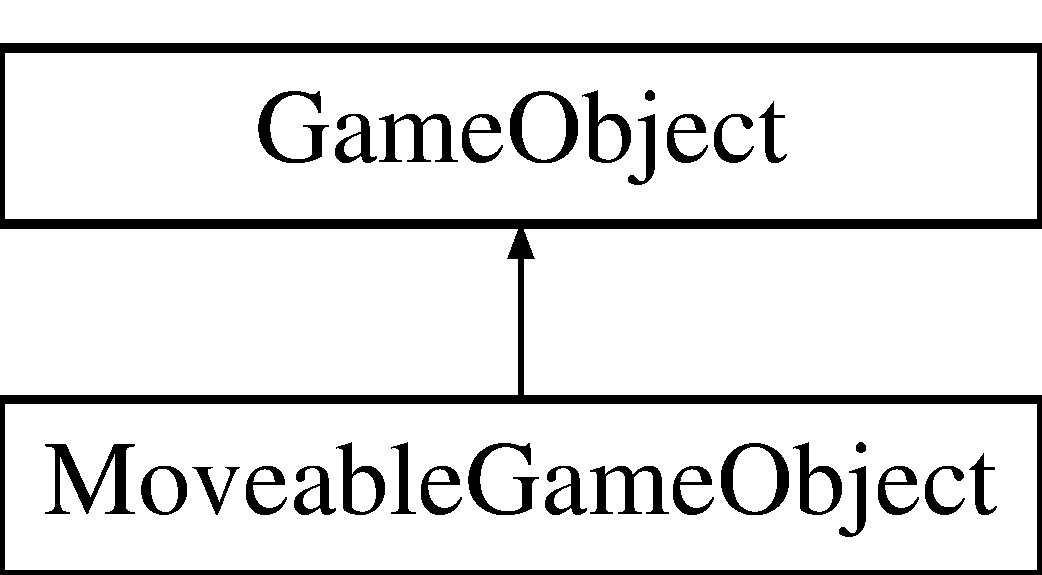
\includegraphics[height=2cm]{classMoveableGameObject}
\end{center}
\end{figure}
\subsection*{Public Member Functions}
\begin{DoxyCompactItemize}
\item 
void \hyperlink{classMoveableGameObject_a6110e3bcfb088cfaa53bc81ce220bab1}{draw} (void)
\item 
bool \hyperlink{classMoveableGameObject_af2a5d981743e85b4bd35a90f874b361b}{update} (unsigned int)
\item 
\hypertarget{classMoveableGameObject_a35e6de5de69921201d48989af9310b71}{
{\bfseries MoveableGameObject} (\hyperlink{classWorld}{World} $\ast$, CL\_\-Pointd \&, CL\_\-Angle \&)}
\label{classMoveableGameObject_a35e6de5de69921201d48989af9310b71}

\end{DoxyCompactItemize}


\subsection{Member Function Documentation}
\hypertarget{classMoveableGameObject_a6110e3bcfb088cfaa53bc81ce220bab1}{
\index{MoveableGameObject@{MoveableGameObject}!draw@{draw}}
\index{draw@{draw}!MoveableGameObject@{MoveableGameObject}}
\subsubsection[{draw}]{\setlength{\rightskip}{0pt plus 5cm}void MoveableGameObject::draw (void)\hspace{0.3cm}{\ttfamily  \mbox{[}virtual\mbox{]}}}}
\label{classMoveableGameObject_a6110e3bcfb088cfaa53bc81ce220bab1}
Draws the current static sprite for the object. 

Reimplemented from \hyperlink{classGameObject_abb64143e72358beb808db22182517802}{GameObject}.\hypertarget{classMoveableGameObject_af2a5d981743e85b4bd35a90f874b361b}{
\index{MoveableGameObject@{MoveableGameObject}!update@{update}}
\index{update@{update}!MoveableGameObject@{MoveableGameObject}}
\subsubsection[{update}]{\setlength{\rightskip}{0pt plus 5cm}bool MoveableGameObject::update (unsigned int {\em time\_\-elapsed\_\-ms})\hspace{0.3cm}{\ttfamily  \mbox{[}virtual\mbox{]}}}}
\label{classMoveableGameObject_af2a5d981743e85b4bd35a90f874b361b}
Updates any animation in the current sprite. 

Reimplemented from \hyperlink{classGameObject_ad2f3cd5d1f5a11b237507cd3ee98b95d}{GameObject}.

The documentation for this class was generated from the following files:\begin{DoxyCompactItemize}
\item 
source/game/\hyperlink{MoveableGameObject_8h}{MoveableGameObject.h}\item 
source/game/\hyperlink{MoveableGameObject_8cpp}{MoveableGameObject.cpp}\end{DoxyCompactItemize}

\hypertarget{structdlib_1_1is__convertible_1_1no__type}{
\section{dlib::is\_\-convertible$<$ from, to $>$::no\_\-type Struct Reference}
\label{structdlib_1_1is__convertible_1_1no__type}\index{dlib::is\_\-convertible::no\_\-type@{dlib::is\_\-convertible::no\_\-type}}
}
\subsection*{Public Attributes}
\begin{DoxyCompactItemize}
\item 
\hypertarget{structdlib_1_1is__convertible_1_1no__type_a8cb9eb6bdb378eff2c1467069316443a}{
\hyperlink{structdlib_1_1is__convertible_1_1yes__type}{yes\_\-type} {\bfseries a} \mbox{[}2\mbox{]}}
\label{structdlib_1_1is__convertible_1_1no__type_a8cb9eb6bdb378eff2c1467069316443a}

\end{DoxyCompactItemize}
\subsubsection*{template$<$typename from, typename to$>$ struct dlib::is\_\-convertible$<$ from, to $>$::no\_\-type}



The documentation for this struct was generated from the following file:\begin{DoxyCompactItemize}
\item 
source/dlib/algs.h\end{DoxyCompactItemize}

\hypertarget{classboost_1_1noncopyable___1_1noncopyable}{
\section{boost::noncopyable\_\-::noncopyable Class Reference}
\label{classboost_1_1noncopyable___1_1noncopyable}\index{boost::noncopyable\_\-::noncopyable@{boost::noncopyable\_\-::noncopyable}}
}
\subsection*{Protected Member Functions}
\begin{DoxyCompactItemize}
\item 
\hyperlink{classboost_1_1noncopyable___1_1noncopyable_a39380533ef795a888a120ec0b1eb9333}{noncopyable} ()
\end{DoxyCompactItemize}


\subsection{Constructor \& Destructor Documentation}
\hypertarget{classboost_1_1noncopyable___1_1noncopyable_a39380533ef795a888a120ec0b1eb9333}{
\index{boost::noncopyable\_\-::noncopyable@{boost::noncopyable\_\-::noncopyable}!noncopyable@{noncopyable}}
\index{noncopyable@{noncopyable}!boost::noncopyable_::noncopyable@{boost::noncopyable\_\-::noncopyable}}
\subsubsection[{noncopyable}]{\setlength{\rightskip}{0pt plus 5cm}boost::noncopyable\_\-::noncopyable::noncopyable ()\hspace{0.3cm}{\ttfamily  \mbox{[}inline, protected\mbox{]}}}}
\label{classboost_1_1noncopyable___1_1noncopyable_a39380533ef795a888a120ec0b1eb9333}
This class makes it easier to declare a class as non-\/copyable. If you want to make an object that can't be copied just inherit from this object. ! 

The documentation for this class was generated from the following file:\begin{DoxyCompactItemize}
\item 
source/dlib/noncopyable.h\end{DoxyCompactItemize}

\hypertarget{classOption}{
\section{Option Class Reference}
\label{classOption}\index{Option@{Option}}
}
\subsection*{Public Member Functions}
\begin{DoxyCompactItemize}
\item 
\hypertarget{classOption_a3cd7af3fd09c247d01e6725e24a91ea2}{
{\bfseries Option} (\hyperlink{classPlot}{Plot} $\ast$, const CL\_\-DomElement \&)}
\label{classOption_a3cd7af3fd09c247d01e6725e24a91ea2}

\item 
\hypertarget{classOption_aa4598f77bf8564c48e3e7b82cd06ed7f}{
int {\bfseries getId} (void)}
\label{classOption_aa4598f77bf8564c48e3e7b82cd06ed7f}

\end{DoxyCompactItemize}


The documentation for this class was generated from the following files:\begin{DoxyCompactItemize}
\item 
mystery\_\-xml/Option.h\item 
mystery\_\-xml/Option.cpp\end{DoxyCompactItemize}

\hypertarget{classOptions}{
\section{Options Class Reference}
\label{classOptions}\index{Options@{Options}}
}
\subsection*{Public Member Functions}
\begin{DoxyCompactItemize}
\item 
\hypertarget{classOptions_a7724e0a467faf1a7538c7345400c0e3f}{
{\bfseries Options} (\hyperlink{classPlot}{Plot} $\ast$, const CL\_\-DomElement \&)}
\label{classOptions_a7724e0a467faf1a7538c7345400c0e3f}

\item 
\hyperlink{classResult}{Result} \hyperlink{classOptions_af944d166a9889b2ff225fe163ab92671}{select} (void)
\end{DoxyCompactItemize}


\subsection{Member Function Documentation}
\hypertarget{classOptions_af944d166a9889b2ff225fe163ab92671}{
\index{Options@{Options}!select@{select}}
\index{select@{select}!Options@{Options}}
\subsubsection[{select}]{\setlength{\rightskip}{0pt plus 5cm}{\bf Result} Options::select (void)}}
\label{classOptions_af944d166a9889b2ff225fe163ab92671}
Picks a value based on weights and parameters. 

The documentation for this class was generated from the following files:\begin{DoxyCompactItemize}
\item 
source/mystery\_\-xml/\hyperlink{Options_8h}{Options.h}\item 
source/mystery\_\-xml/\hyperlink{Options_8cpp}{Options.cpp}\end{DoxyCompactItemize}

\hypertarget{classOverlay}{
\section{Overlay Class Reference}
\label{classOverlay}\index{Overlay@{Overlay}}
}
Inheritance diagram for Overlay:\begin{figure}[H]
\begin{center}
\leavevmode
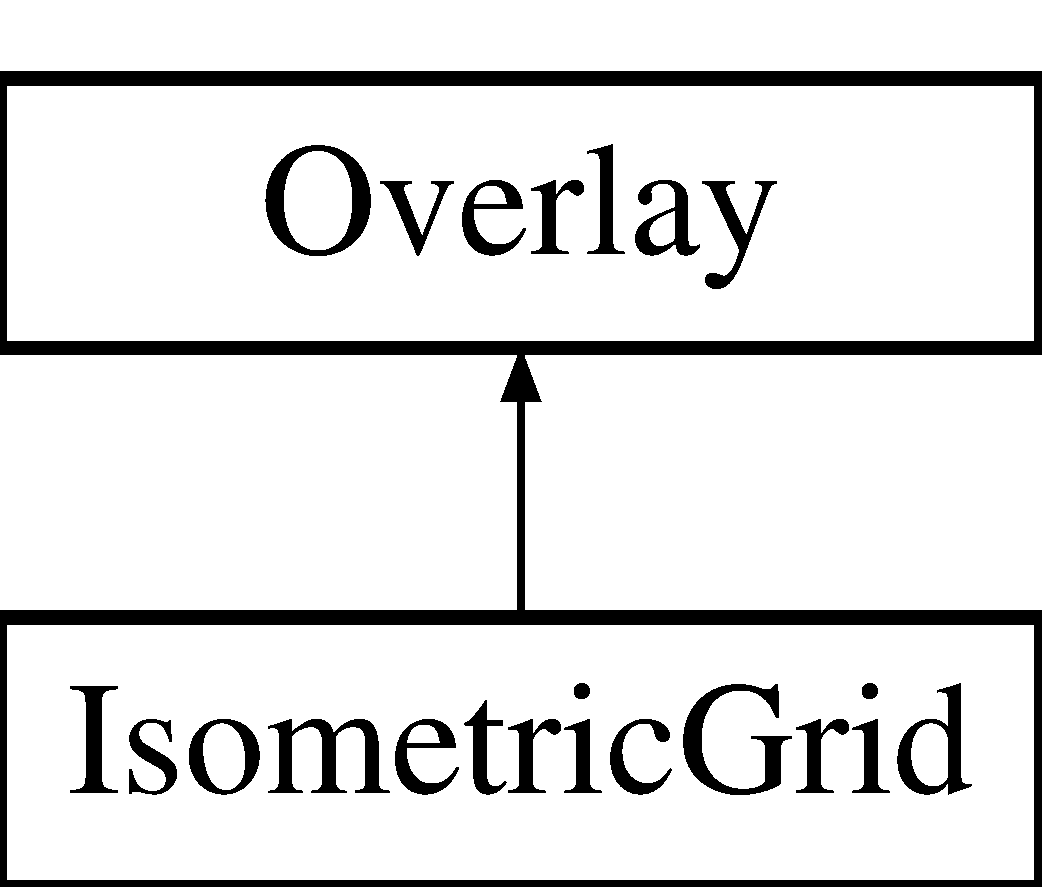
\includegraphics[height=2cm]{classOverlay}
\end{center}
\end{figure}
\subsection*{Public Member Functions}
\begin{DoxyCompactItemize}
\item 
\hypertarget{classOverlay_aecb2ad2cea6041a1b1e332e041daeb13}{
{\bfseries Overlay} (\hyperlink{classWorld}{World} $\ast$)}
\label{classOverlay_aecb2ad2cea6041a1b1e332e041daeb13}

\item 
\hypertarget{classOverlay_a384639128697df8c44c3801ae9212be3}{
virtual void {\bfseries draw} ()=0}
\label{classOverlay_a384639128697df8c44c3801ae9212be3}

\end{DoxyCompactItemize}
\subsection*{Protected Attributes}
\begin{DoxyCompactItemize}
\item 
\hypertarget{classOverlay_aa0de2439856791f770c9e2e9bdc5b613}{
\hyperlink{classWorld}{World} $\ast$ {\bfseries world}}
\label{classOverlay_aa0de2439856791f770c9e2e9bdc5b613}

\end{DoxyCompactItemize}


The documentation for this class was generated from the following files:\begin{DoxyCompactItemize}
\item 
source/game/\hyperlink{Overlay_8h}{Overlay.h}\item 
source/game/\hyperlink{Overlay_8cpp}{Overlay.cpp}\end{DoxyCompactItemize}

\hypertarget{classdlib_1_1pipe}{
\section{dlib::pipe$<$ T $>$ Class Template Reference}
\label{classdlib_1_1pipe}\index{dlib::pipe@{dlib::pipe}}
}
\subsection*{Public Types}
\begin{DoxyCompactItemize}
\item 
\hypertarget{classdlib_1_1pipe_a4bf0a8af96d3862476be943867b52c2d}{
typedef pipe\_\-kernel\_\-1$<$ T $>$ {\bfseries kernel\_\-1a}}
\label{classdlib_1_1pipe_a4bf0a8af96d3862476be943867b52c2d}

\end{DoxyCompactItemize}
\subsubsection*{template$<$typename T$>$ class dlib::pipe$<$ T $>$}



The documentation for this class was generated from the following file:\begin{DoxyCompactItemize}
\item 
source/dlib/pipe.h\end{DoxyCompactItemize}

\hypertarget{structdlib_1_1pixel__traits_3_01bgr__pixel_01_4}{
\section{dlib::pixel\_\-traits$<$ bgr\_\-pixel $>$ Struct Template Reference}
\label{structdlib_1_1pixel__traits_3_01bgr__pixel_01_4}\index{dlib::pixel\_\-traits$<$ bgr\_\-pixel $>$@{dlib::pixel\_\-traits$<$ bgr\_\-pixel $>$}}
}
\subsection*{Static Public Member Functions}
\begin{DoxyCompactItemize}
\item 
\hypertarget{structdlib_1_1pixel__traits_3_01bgr__pixel_01_4_aca46cbf44ecfda9d55892ea857c8981a}{
static unsigned long {\bfseries max} ()}
\label{structdlib_1_1pixel__traits_3_01bgr__pixel_01_4_aca46cbf44ecfda9d55892ea857c8981a}

\end{DoxyCompactItemize}
\subsection*{Static Public Attributes}
\begin{DoxyCompactItemize}
\item 
\hypertarget{structdlib_1_1pixel__traits_3_01bgr__pixel_01_4_ae64be3fe89fc84125ebd87b801cb9622}{
static const bool {\bfseries rgb} = true}
\label{structdlib_1_1pixel__traits_3_01bgr__pixel_01_4_ae64be3fe89fc84125ebd87b801cb9622}

\item 
\hypertarget{structdlib_1_1pixel__traits_3_01bgr__pixel_01_4_a2a0e68764c422ca8409a009ee9f4559b}{
static const bool {\bfseries rgb\_\-alpha} = false}
\label{structdlib_1_1pixel__traits_3_01bgr__pixel_01_4_a2a0e68764c422ca8409a009ee9f4559b}

\item 
\hypertarget{structdlib_1_1pixel__traits_3_01bgr__pixel_01_4_a29ae2efc247f331ba87a9ece96db7c62}{
static const bool {\bfseries grayscale} = false}
\label{structdlib_1_1pixel__traits_3_01bgr__pixel_01_4_a29ae2efc247f331ba87a9ece96db7c62}

\item 
\hypertarget{structdlib_1_1pixel__traits_3_01bgr__pixel_01_4_a20bd2668bdb771f16944a2eed78f144a}{
static const bool {\bfseries hsi} = false}
\label{structdlib_1_1pixel__traits_3_01bgr__pixel_01_4_a20bd2668bdb771f16944a2eed78f144a}

\item 
\hypertarget{structdlib_1_1pixel__traits_3_01bgr__pixel_01_4_a4a89b7bad527dad5013ba70be9c6dd0e}{
static const long {\bfseries num} = 3}
\label{structdlib_1_1pixel__traits_3_01bgr__pixel_01_4_a4a89b7bad527dad5013ba70be9c6dd0e}

\item 
\hypertarget{structdlib_1_1pixel__traits_3_01bgr__pixel_01_4_a062aba3e7bc7feaf2e18bcb3daf5fd1c}{
static const bool {\bfseries has\_\-alpha} = false}
\label{structdlib_1_1pixel__traits_3_01bgr__pixel_01_4_a062aba3e7bc7feaf2e18bcb3daf5fd1c}

\end{DoxyCompactItemize}
\subsubsection*{template$<$$>$ struct dlib::pixel\_\-traits$<$ bgr\_\-pixel $>$}



The documentation for this struct was generated from the following file:\begin{DoxyCompactItemize}
\item 
source/dlib/pixel.h\end{DoxyCompactItemize}

\hypertarget{structdlib_1_1pixel__traits_3_01hsi__pixel_01_4}{
\section{dlib::pixel\_\-traits$<$ hsi\_\-pixel $>$ Struct Template Reference}
\label{structdlib_1_1pixel__traits_3_01hsi__pixel_01_4}\index{dlib::pixel\_\-traits$<$ hsi\_\-pixel $>$@{dlib::pixel\_\-traits$<$ hsi\_\-pixel $>$}}
}
\subsection*{Static Public Member Functions}
\begin{DoxyCompactItemize}
\item 
\hypertarget{structdlib_1_1pixel__traits_3_01hsi__pixel_01_4_a09608d99b5b5779622e4c0a25fece089}{
static unsigned long {\bfseries max} ()}
\label{structdlib_1_1pixel__traits_3_01hsi__pixel_01_4_a09608d99b5b5779622e4c0a25fece089}

\end{DoxyCompactItemize}
\subsection*{Static Public Attributes}
\begin{DoxyCompactItemize}
\item 
\hypertarget{structdlib_1_1pixel__traits_3_01hsi__pixel_01_4_af6b191b1f9c11c43722fa848cffd00d5}{
static const bool {\bfseries rgb} = false}
\label{structdlib_1_1pixel__traits_3_01hsi__pixel_01_4_af6b191b1f9c11c43722fa848cffd00d5}

\item 
\hypertarget{structdlib_1_1pixel__traits_3_01hsi__pixel_01_4_a072504a7d58fd17b2421560dcacc25d4}{
static const bool {\bfseries rgb\_\-alpha} = false}
\label{structdlib_1_1pixel__traits_3_01hsi__pixel_01_4_a072504a7d58fd17b2421560dcacc25d4}

\item 
\hypertarget{structdlib_1_1pixel__traits_3_01hsi__pixel_01_4_a02e32045f3fa3056470f0670244bd55e}{
static const bool {\bfseries grayscale} = false}
\label{structdlib_1_1pixel__traits_3_01hsi__pixel_01_4_a02e32045f3fa3056470f0670244bd55e}

\item 
\hypertarget{structdlib_1_1pixel__traits_3_01hsi__pixel_01_4_a67ac73ee28e00179d70bd4a22ea39af4}{
static const bool {\bfseries hsi} = true}
\label{structdlib_1_1pixel__traits_3_01hsi__pixel_01_4_a67ac73ee28e00179d70bd4a22ea39af4}

\item 
\hypertarget{structdlib_1_1pixel__traits_3_01hsi__pixel_01_4_a0eaba4f435662b7acf43356c126bfd1a}{
static const long {\bfseries num} = 3}
\label{structdlib_1_1pixel__traits_3_01hsi__pixel_01_4_a0eaba4f435662b7acf43356c126bfd1a}

\item 
\hypertarget{structdlib_1_1pixel__traits_3_01hsi__pixel_01_4_a693f2baa6c2dfb42326b768c612fc4cd}{
static const bool {\bfseries has\_\-alpha} = false}
\label{structdlib_1_1pixel__traits_3_01hsi__pixel_01_4_a693f2baa6c2dfb42326b768c612fc4cd}

\end{DoxyCompactItemize}
\subsubsection*{template$<$$>$ struct dlib::pixel\_\-traits$<$ hsi\_\-pixel $>$}



The documentation for this struct was generated from the following file:\begin{DoxyCompactItemize}
\item 
source/dlib/pixel.h\end{DoxyCompactItemize}

\hypertarget{structdlib_1_1pixel__traits_3_01rgb__alpha__pixel_01_4}{
\section{dlib::pixel\_\-traits$<$ rgb\_\-alpha\_\-pixel $>$ Struct Template Reference}
\label{structdlib_1_1pixel__traits_3_01rgb__alpha__pixel_01_4}\index{dlib::pixel\_\-traits$<$ rgb\_\-alpha\_\-pixel $>$@{dlib::pixel\_\-traits$<$ rgb\_\-alpha\_\-pixel $>$}}
}
\subsection*{Static Public Member Functions}
\begin{DoxyCompactItemize}
\item 
\hypertarget{structdlib_1_1pixel__traits_3_01rgb__alpha__pixel_01_4_a8e618969b2c20aaf3104bbae4dcff575}{
static unsigned long {\bfseries max} ()}
\label{structdlib_1_1pixel__traits_3_01rgb__alpha__pixel_01_4_a8e618969b2c20aaf3104bbae4dcff575}

\end{DoxyCompactItemize}
\subsection*{Static Public Attributes}
\begin{DoxyCompactItemize}
\item 
\hypertarget{structdlib_1_1pixel__traits_3_01rgb__alpha__pixel_01_4_aed238eef6e9c1362eef1af6906251380}{
static const bool {\bfseries rgb} = false}
\label{structdlib_1_1pixel__traits_3_01rgb__alpha__pixel_01_4_aed238eef6e9c1362eef1af6906251380}

\item 
\hypertarget{structdlib_1_1pixel__traits_3_01rgb__alpha__pixel_01_4_abe68a247c056dee66bc1c430fd426430}{
static const bool {\bfseries rgb\_\-alpha} = true}
\label{structdlib_1_1pixel__traits_3_01rgb__alpha__pixel_01_4_abe68a247c056dee66bc1c430fd426430}

\item 
\hypertarget{structdlib_1_1pixel__traits_3_01rgb__alpha__pixel_01_4_af6817e9710ffb3bbd3ce83e05f9541cd}{
static const bool {\bfseries grayscale} = false}
\label{structdlib_1_1pixel__traits_3_01rgb__alpha__pixel_01_4_af6817e9710ffb3bbd3ce83e05f9541cd}

\item 
\hypertarget{structdlib_1_1pixel__traits_3_01rgb__alpha__pixel_01_4_ad4a92f9b421618c75432eef0aede06db}{
static const bool {\bfseries hsi} = false}
\label{structdlib_1_1pixel__traits_3_01rgb__alpha__pixel_01_4_ad4a92f9b421618c75432eef0aede06db}

\item 
\hypertarget{structdlib_1_1pixel__traits_3_01rgb__alpha__pixel_01_4_a440d908b0bb2621432309391ce81d6f7}{
static const long {\bfseries num} = 4}
\label{structdlib_1_1pixel__traits_3_01rgb__alpha__pixel_01_4_a440d908b0bb2621432309391ce81d6f7}

\item 
\hypertarget{structdlib_1_1pixel__traits_3_01rgb__alpha__pixel_01_4_ae5f039f49856a73a92eac77430c71b6e}{
static const bool {\bfseries has\_\-alpha} = true}
\label{structdlib_1_1pixel__traits_3_01rgb__alpha__pixel_01_4_ae5f039f49856a73a92eac77430c71b6e}

\end{DoxyCompactItemize}
\subsubsection*{template$<$$>$ struct dlib::pixel\_\-traits$<$ rgb\_\-alpha\_\-pixel $>$}



The documentation for this struct was generated from the following file:\begin{DoxyCompactItemize}
\item 
source/dlib/pixel.h\end{DoxyCompactItemize}

\hypertarget{structdlib_1_1pixel__traits_3_01rgb__pixel_01_4}{
\section{dlib::pixel\_\-traits$<$ rgb\_\-pixel $>$ Struct Template Reference}
\label{structdlib_1_1pixel__traits_3_01rgb__pixel_01_4}\index{dlib::pixel\_\-traits$<$ rgb\_\-pixel $>$@{dlib::pixel\_\-traits$<$ rgb\_\-pixel $>$}}
}


{\ttfamily \#include $<$pixel.h$>$}\subsection*{Static Public Member Functions}
\begin{DoxyCompactItemize}
\item 
\hypertarget{structdlib_1_1pixel__traits_3_01rgb__pixel_01_4_af3db9d5d63794f2fc947e7e9bc6315c7}{
static unsigned long {\bfseries max} ()}
\label{structdlib_1_1pixel__traits_3_01rgb__pixel_01_4_af3db9d5d63794f2fc947e7e9bc6315c7}

\end{DoxyCompactItemize}
\subsection*{Static Public Attributes}
\begin{DoxyCompactItemize}
\item 
\hypertarget{structdlib_1_1pixel__traits_3_01rgb__pixel_01_4_a0b79e04ebcd17ddbda0e53759e3dc1cb}{
static const bool {\bfseries rgb} = true}
\label{structdlib_1_1pixel__traits_3_01rgb__pixel_01_4_a0b79e04ebcd17ddbda0e53759e3dc1cb}

\item 
\hypertarget{structdlib_1_1pixel__traits_3_01rgb__pixel_01_4_a8c7b8ef75bac6d6b3a69a224cf9afde7}{
static const bool {\bfseries rgb\_\-alpha} = false}
\label{structdlib_1_1pixel__traits_3_01rgb__pixel_01_4_a8c7b8ef75bac6d6b3a69a224cf9afde7}

\item 
\hypertarget{structdlib_1_1pixel__traits_3_01rgb__pixel_01_4_aa5ce2a2349b380544692015776f0ca96}{
static const bool {\bfseries grayscale} = false}
\label{structdlib_1_1pixel__traits_3_01rgb__pixel_01_4_aa5ce2a2349b380544692015776f0ca96}

\item 
\hypertarget{structdlib_1_1pixel__traits_3_01rgb__pixel_01_4_ac9f647ad44676773637cca8d17f3fdf3}{
static const bool {\bfseries hsi} = false}
\label{structdlib_1_1pixel__traits_3_01rgb__pixel_01_4_ac9f647ad44676773637cca8d17f3fdf3}

\item 
\hypertarget{structdlib_1_1pixel__traits_3_01rgb__pixel_01_4_afe1a8263d3287379b2a6770f03fb38be}{
static const long {\bfseries num} = 3}
\label{structdlib_1_1pixel__traits_3_01rgb__pixel_01_4_afe1a8263d3287379b2a6770f03fb38be}

\item 
\hypertarget{structdlib_1_1pixel__traits_3_01rgb__pixel_01_4_a6cac7160f3fad29a6732f1158cba8268}{
static const bool {\bfseries has\_\-alpha} = false}
\label{structdlib_1_1pixel__traits_3_01rgb__pixel_01_4_a6cac7160f3fad29a6732f1158cba8268}

\end{DoxyCompactItemize}


\subsection{Detailed Description}
\subsubsection*{template$<$$>$ struct dlib::pixel\_\-traits$<$ rgb\_\-pixel $>$}

provides deserialization support for the \hyperlink{structdlib_1_1hsi__pixel}{hsi\_\-pixel} struct ! 

The documentation for this struct was generated from the following file:\begin{DoxyCompactItemize}
\item 
source/dlib/pixel.h\end{DoxyCompactItemize}

\hypertarget{structdlib_1_1pixel__traits_3_01unsigned_01char_01_4}{
\section{dlib::pixel\_\-traits$<$ unsigned char $>$ Struct Template Reference}
\label{structdlib_1_1pixel__traits_3_01unsigned_01char_01_4}\index{dlib::pixel\_\-traits$<$ unsigned char $>$@{dlib::pixel\_\-traits$<$ unsigned char $>$}}
}
Inheritance diagram for dlib::pixel\_\-traits$<$ unsigned char $>$::\begin{figure}[H]
\begin{center}
\leavevmode
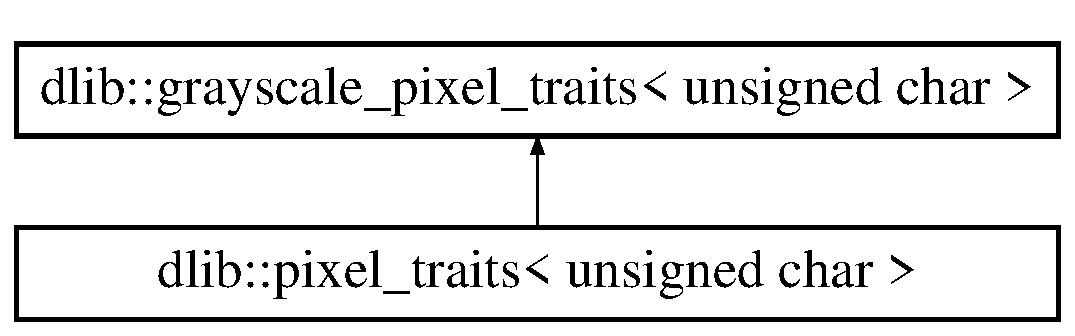
\includegraphics[height=2cm]{structdlib_1_1pixel__traits_3_01unsigned_01char_01_4}
\end{center}
\end{figure}
\subsubsection*{template$<$$>$ struct dlib::pixel\_\-traits$<$ unsigned char $>$}



The documentation for this struct was generated from the following file:\begin{DoxyCompactItemize}
\item 
source/dlib/pixel.h\end{DoxyCompactItemize}

\hypertarget{structdlib_1_1pixel__traits_3_01unsigned_01int_01_4}{
\section{dlib::pixel\_\-traits$<$ unsigned int $>$ Struct Template Reference}
\label{structdlib_1_1pixel__traits_3_01unsigned_01int_01_4}\index{dlib::pixel\_\-traits$<$ unsigned int $>$@{dlib::pixel\_\-traits$<$ unsigned int $>$}}
}
Inheritance diagram for dlib::pixel\_\-traits$<$ unsigned int $>$::\begin{figure}[H]
\begin{center}
\leavevmode
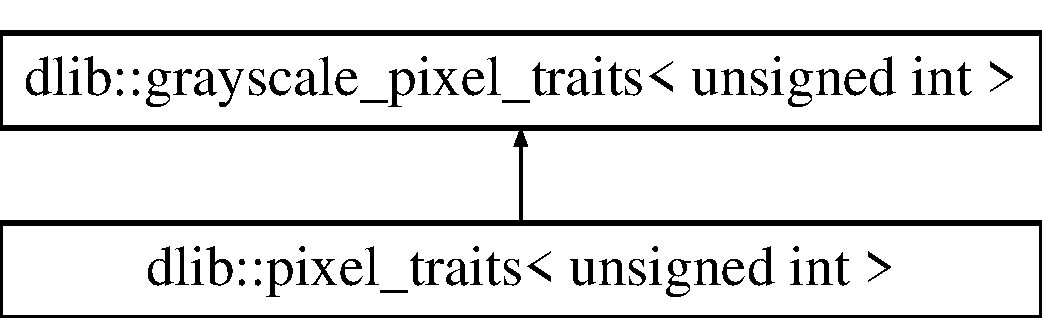
\includegraphics[height=2cm]{structdlib_1_1pixel__traits_3_01unsigned_01int_01_4}
\end{center}
\end{figure}
\subsubsection*{template$<$$>$ struct dlib::pixel\_\-traits$<$ unsigned int $>$}



The documentation for this struct was generated from the following file:\begin{DoxyCompactItemize}
\item 
source/dlib/pixel.h\end{DoxyCompactItemize}

\hypertarget{structdlib_1_1pixel__traits_3_01unsigned_01long_01_4}{
\section{dlib::pixel\_\-traits$<$ unsigned long $>$ Struct Template Reference}
\label{structdlib_1_1pixel__traits_3_01unsigned_01long_01_4}\index{dlib::pixel\_\-traits$<$ unsigned long $>$@{dlib::pixel\_\-traits$<$ unsigned long $>$}}
}
Inheritance diagram for dlib::pixel\_\-traits$<$ unsigned long $>$::\begin{figure}[H]
\begin{center}
\leavevmode
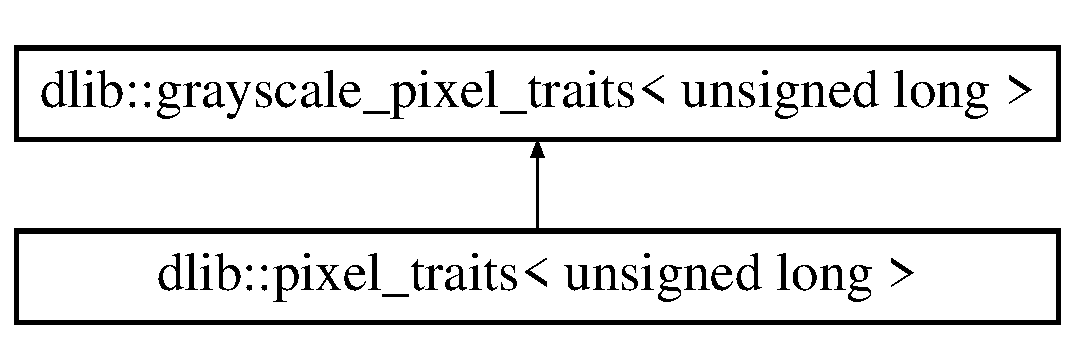
\includegraphics[height=2cm]{structdlib_1_1pixel__traits_3_01unsigned_01long_01_4}
\end{center}
\end{figure}
\subsubsection*{template$<$$>$ struct dlib::pixel\_\-traits$<$ unsigned long $>$}



The documentation for this struct was generated from the following file:\begin{DoxyCompactItemize}
\item 
source/dlib/pixel.h\end{DoxyCompactItemize}

\hypertarget{structdlib_1_1pixel__traits_3_01unsigned_01short_01_4}{
\section{dlib::pixel\_\-traits$<$ unsigned short $>$ Struct Template Reference}
\label{structdlib_1_1pixel__traits_3_01unsigned_01short_01_4}\index{dlib::pixel\_\-traits$<$ unsigned short $>$@{dlib::pixel\_\-traits$<$ unsigned short $>$}}
}
Inheritance diagram for dlib::pixel\_\-traits$<$ unsigned short $>$::\begin{figure}[H]
\begin{center}
\leavevmode
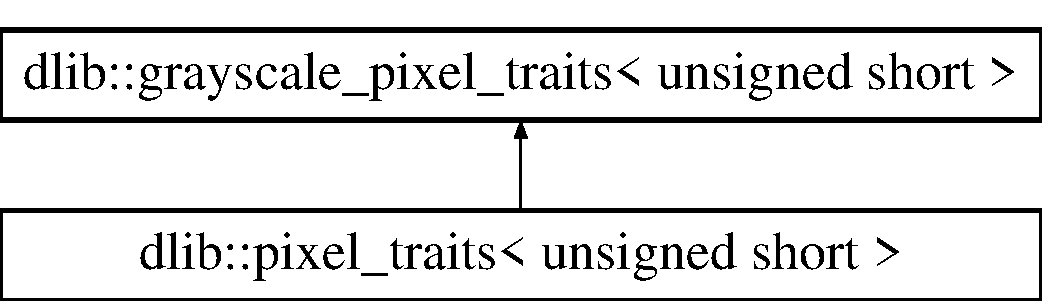
\includegraphics[height=2cm]{structdlib_1_1pixel__traits_3_01unsigned_01short_01_4}
\end{center}
\end{figure}
\subsubsection*{template$<$$>$ struct dlib::pixel\_\-traits$<$ unsigned short $>$}



The documentation for this struct was generated from the following file:\begin{DoxyCompactItemize}
\item 
source/dlib/pixel.h\end{DoxyCompactItemize}

\hypertarget{classPlayerCharacter}{
\section{PlayerCharacter Class Reference}
\label{classPlayerCharacter}\index{PlayerCharacter@{PlayerCharacter}}
}
Inheritance diagram for PlayerCharacter::\begin{figure}[H]
\begin{center}
\leavevmode
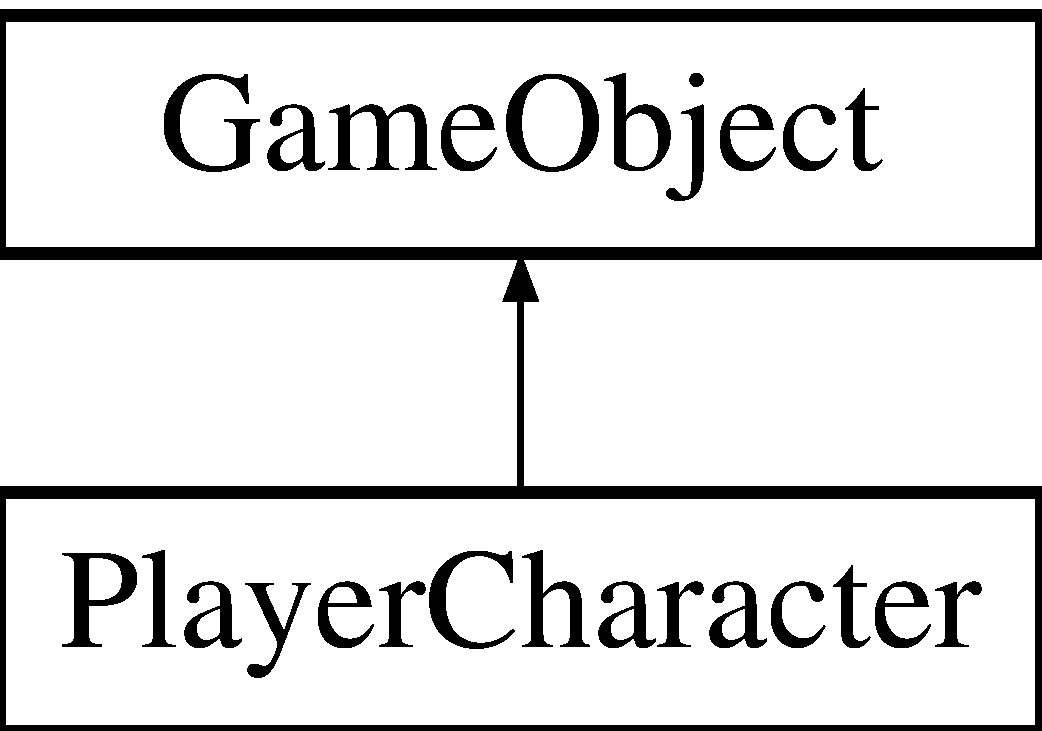
\includegraphics[height=2cm]{classPlayerCharacter}
\end{center}
\end{figure}
\subsection*{Public Member Functions}
\begin{DoxyCompactItemize}
\item 
\hypertarget{classPlayerCharacter_a0207723ef3dc387dcf80b01839715d31}{
{\bfseries PlayerCharacter} (\hyperlink{classWorld}{World} $\ast$, CL\_\-Pointd \&, CL\_\-Angle \&)}
\label{classPlayerCharacter_a0207723ef3dc387dcf80b01839715d31}

\end{DoxyCompactItemize}


The documentation for this class was generated from the following files:\begin{DoxyCompactItemize}
\item 
source/game/\hyperlink{PlayerCharacter_8h}{PlayerCharacter.h}\item 
source/game/\hyperlink{PlayerCharacter_8cpp}{PlayerCharacter.cpp}\end{DoxyCompactItemize}

\hypertarget{classPlot}{
\section{Plot Class Reference}
\label{classPlot}\index{Plot@{Plot}}
}


{\ttfamily \#include $<$Plot.h$>$}\subsection*{Public Member Functions}
\begin{DoxyCompactItemize}
\item 
\hyperlink{classPlot_a836271d0487e811f66768dadb44e4548}{Plot} (const char $\ast$)
\item 
void \hyperlink{classPlot_abdaa02f5857205d8eda001462be0d9f7}{addOption} (\hyperlink{classOption}{Option} $\ast$)
\end{DoxyCompactItemize}


\subsection{Detailed Description}
The plot class is use to parse the plot element in the mystery\_\-xml library. 

\subsection{Constructor \& Destructor Documentation}
\hypertarget{classPlot_a836271d0487e811f66768dadb44e4548}{
\index{Plot@{Plot}!Plot@{Plot}}
\index{Plot@{Plot}!Plot@{Plot}}
\subsubsection[{Plot}]{\setlength{\rightskip}{0pt plus 5cm}Plot::Plot (const char $\ast$ {\em filename})}}
\label{classPlot_a836271d0487e811f66768dadb44e4548}
Constructs a tree from the specified XML file. 

\subsection{Member Function Documentation}
\hypertarget{classPlot_abdaa02f5857205d8eda001462be0d9f7}{
\index{Plot@{Plot}!addOption@{addOption}}
\index{addOption@{addOption}!Plot@{Plot}}
\subsubsection[{addOption}]{\setlength{\rightskip}{0pt plus 5cm}void Plot::addOption ({\bf Option} $\ast$ {\em option})}}
\label{classPlot_abdaa02f5857205d8eda001462be0d9f7}
Adds the \hyperlink{classOption}{Option} object to the map accessible by index. 

The documentation for this class was generated from the following files:\begin{DoxyCompactItemize}
\item 
mystery\_\-xml/Plot.h\item 
mystery\_\-xml/Plot.cpp\end{DoxyCompactItemize}

\hypertarget{classProgram}{
\section{Program Class Reference}
\label{classProgram}\index{Program@{Program}}
}
\subsection*{Static Public Member Functions}
\begin{DoxyCompactItemize}
\item 
\hypertarget{classProgram_a97eed8197e64916a57f1d89477932d7a}{
static int {\bfseries main} (const std::vector$<$ CL\_\-String $>$ \&args)}
\label{classProgram_a97eed8197e64916a57f1d89477932d7a}

\end{DoxyCompactItemize}


The documentation for this class was generated from the following file:\begin{DoxyCompactItemize}
\item 
isometric.cpp\end{DoxyCompactItemize}

\hypertarget{classdlib_1_1queue}{
\section{dlib::queue$<$ T, mem\_\-manager $>$ Class Template Reference}
\label{classdlib_1_1queue}\index{dlib::queue@{dlib::queue}}
}
\subsection*{Public Types}
\begin{DoxyCompactItemize}
\item 
\hypertarget{classdlib_1_1queue_a14ee6503764b6c9f9afa407c364857ef}{
typedef queue\_\-kernel\_\-1$<$ T, mem\_\-manager $>$ {\bfseries kernel\_\-1a}}
\label{classdlib_1_1queue_a14ee6503764b6c9f9afa407c364857ef}

\item 
\hypertarget{classdlib_1_1queue_a7ab77eeb5d1a184eb9646181ebeac3e6}{
typedef queue\_\-kernel\_\-c$<$ kernel\_\-1a $>$ {\bfseries kernel\_\-1a\_\-c}}
\label{classdlib_1_1queue_a7ab77eeb5d1a184eb9646181ebeac3e6}

\item 
\hypertarget{classdlib_1_1queue_a103481f71a51167889230b6f01ad4609}{
typedef queue\_\-kernel\_\-2$<$ T, 20, mem\_\-manager $>$ {\bfseries kernel\_\-2a}}
\label{classdlib_1_1queue_a103481f71a51167889230b6f01ad4609}

\item 
\hypertarget{classdlib_1_1queue_a4e7d41c708ce943321b7d8626f1e11c7}{
typedef queue\_\-kernel\_\-c$<$ kernel\_\-2a $>$ {\bfseries kernel\_\-2a\_\-c}}
\label{classdlib_1_1queue_a4e7d41c708ce943321b7d8626f1e11c7}

\item 
\hypertarget{classdlib_1_1queue_a2c093dccb36ea9a77127f2a5ab5356a0}{
typedef queue\_\-kernel\_\-2$<$ T, 100, mem\_\-manager $>$ {\bfseries kernel\_\-2b}}
\label{classdlib_1_1queue_a2c093dccb36ea9a77127f2a5ab5356a0}

\item 
\hypertarget{classdlib_1_1queue_a29bc94bd114f2f07e6db9b09abd19812}{
typedef queue\_\-kernel\_\-c$<$ kernel\_\-2b $>$ {\bfseries kernel\_\-2b\_\-c}}
\label{classdlib_1_1queue_a29bc94bd114f2f07e6db9b09abd19812}

\item 
\hypertarget{classdlib_1_1queue_a1b0ef2aa0008b998ab6c2e5044d152a6}{
typedef queue\_\-sort\_\-1$<$ kernel\_\-1a $>$ {\bfseries sort\_\-1a}}
\label{classdlib_1_1queue_a1b0ef2aa0008b998ab6c2e5044d152a6}

\item 
\hypertarget{classdlib_1_1queue_ae2102477620a2276d61c4a8921ccd6b3}{
typedef queue\_\-sort\_\-1$<$ kernel\_\-1a\_\-c $>$ {\bfseries sort\_\-1a\_\-c}}
\label{classdlib_1_1queue_ae2102477620a2276d61c4a8921ccd6b3}

\item 
\hypertarget{classdlib_1_1queue_a3c225e24e6bca0a6c808ac2bd7a86af0}{
typedef queue\_\-sort\_\-1$<$ kernel\_\-2a $>$ {\bfseries sort\_\-1b}}
\label{classdlib_1_1queue_a3c225e24e6bca0a6c808ac2bd7a86af0}

\item 
\hypertarget{classdlib_1_1queue_a83fb0e16148d97bdad71501cfc45b22d}{
typedef queue\_\-sort\_\-1$<$ kernel\_\-2a\_\-c $>$ {\bfseries sort\_\-1b\_\-c}}
\label{classdlib_1_1queue_a83fb0e16148d97bdad71501cfc45b22d}

\item 
\hypertarget{classdlib_1_1queue_a4877f1e730d84149cac55e3bba71c7a5}{
typedef queue\_\-sort\_\-1$<$ kernel\_\-2b $>$ {\bfseries sort\_\-1c}}
\label{classdlib_1_1queue_a4877f1e730d84149cac55e3bba71c7a5}

\item 
\hypertarget{classdlib_1_1queue_ab0617c1ac2328e3641bbcfba8d63988c}{
typedef queue\_\-sort\_\-1$<$ kernel\_\-2b\_\-c $>$ {\bfseries sort\_\-1c\_\-c}}
\label{classdlib_1_1queue_ab0617c1ac2328e3641bbcfba8d63988c}

\end{DoxyCompactItemize}
\subsubsection*{template$<$typename T, typename mem\_\-manager = memory\_\-manager$<$char$>$::kernel\_\-1a$>$ class dlib::queue$<$ T, mem\_\-manager $>$}



The documentation for this class was generated from the following file:\begin{DoxyCompactItemize}
\item 
source/dlib/queue.h\end{DoxyCompactItemize}

\hypertarget{classdlib_1_1rand}{
\section{dlib::rand Class Reference}
\label{classdlib_1_1rand}\index{dlib::rand@{dlib::rand}}
}
\subsection*{Public Types}
\begin{DoxyCompactItemize}
\item 
\hypertarget{classdlib_1_1rand_a65c91e0dc68fac0c2a204ac5c465f068}{
typedef rand\_\-kernel\_\-1 {\bfseries kernel\_\-1a}}
\label{classdlib_1_1rand_a65c91e0dc68fac0c2a204ac5c465f068}

\item 
\hypertarget{classdlib_1_1rand_aed991af3ccf458d335819968d1c9c0f1}{
typedef rand\_\-float\_\-1$<$ kernel\_\-1a $>$ {\bfseries float\_\-1a}}
\label{classdlib_1_1rand_aed991af3ccf458d335819968d1c9c0f1}

\end{DoxyCompactItemize}


The documentation for this class was generated from the following file:\begin{DoxyCompactItemize}
\item 
source/dlib/rand.h\end{DoxyCompactItemize}

\hypertarget{classRandomGenerator}{
\section{RandomGenerator Class Reference}
\label{classRandomGenerator}\index{RandomGenerator@{RandomGenerator}}
}


{\ttfamily \#include $<$RandomGenerator.h$>$}\subsection*{Public Member Functions}
\begin{DoxyCompactItemize}
\item 
\hypertarget{classRandomGenerator_addcda615af9b184d61705dacd0cc0a9a}{
{\bfseries RandomGenerator} (unsigned int)}
\label{classRandomGenerator_addcda615af9b184d61705dacd0cc0a9a}

\item 
\hypertarget{classRandomGenerator_ae10cbb24c2728a4d8d441f2774ac8b99}{
double {\bfseries generateFloat} (void)}
\label{classRandomGenerator_ae10cbb24c2728a4d8d441f2774ac8b99}

\end{DoxyCompactItemize}


\subsection{Detailed Description}
This provides random numbers for the 

The documentation for this class was generated from the following files:\begin{DoxyCompactItemize}
\item 
source/game/\hyperlink{RandomGenerator_8h}{RandomGenerator.h}\item 
source/game/\hyperlink{RandomGenerator_8cpp}{RandomGenerator.cpp}\end{DoxyCompactItemize}

\hypertarget{structdlib_1_1std__allocator_1_1rebind}{
\section{dlib::std\_\-allocator$<$ T, M $>$::rebind$<$ U $>$ Struct Template Reference}
\label{structdlib_1_1std__allocator_1_1rebind}\index{dlib::std\_\-allocator::rebind@{dlib::std\_\-allocator::rebind}}
}
\subsection*{Public Types}
\begin{DoxyCompactItemize}
\item 
\hypertarget{structdlib_1_1std__allocator_1_1rebind_a90c3fff2cb39bc8692290016b39610b7}{
typedef \hyperlink{classdlib_1_1std__allocator}{std\_\-allocator}$<$ U, M $>$ {\bfseries other}}
\label{structdlib_1_1std__allocator_1_1rebind_a90c3fff2cb39bc8692290016b39610b7}

\end{DoxyCompactItemize}
\subsubsection*{template$<$typename T, typename M$>$template$<$typename U$>$ struct dlib::std\_\-allocator$<$ T, M $>$::rebind$<$ U $>$}



The documentation for this struct was generated from the following file:\begin{DoxyCompactItemize}
\item 
source/dlib/std\_\-allocator.h\end{DoxyCompactItemize}

\hypertarget{structdlib_1_1std__allocator_3_01void_00_01M_01_4_1_1rebind}{
\section{dlib::std\_\-allocator$<$ void, M $>$::rebind$<$ U $>$ Struct Template Reference}
\label{structdlib_1_1std__allocator_3_01void_00_01M_01_4_1_1rebind}\index{dlib::std\_\-allocator$<$ void, M $>$::rebind@{dlib::std\_\-allocator$<$ void, M $>$::rebind}}
}
\subsection*{Public Types}
\begin{DoxyCompactItemize}
\item 
\hypertarget{structdlib_1_1std__allocator_3_01void_00_01M_01_4_1_1rebind_a01b39f090eda7273c058b0b1b9bb945d}{
typedef \hyperlink{classdlib_1_1std__allocator}{std\_\-allocator}$<$ U, M $>$ {\bfseries other}}
\label{structdlib_1_1std__allocator_3_01void_00_01M_01_4_1_1rebind_a01b39f090eda7273c058b0b1b9bb945d}

\end{DoxyCompactItemize}
\subsubsection*{template$<$typename M$>$template$<$typename U$>$ struct dlib::std\_\-allocator$<$ void, M $>$::rebind$<$ U $>$}



The documentation for this struct was generated from the following file:\begin{DoxyCompactItemize}
\item 
source/dlib/std\_\-allocator.h\end{DoxyCompactItemize}

\hypertarget{classdlib_1_1reference__counter}{
\section{dlib::reference\_\-counter$<$ T, copy $>$ Class Template Reference}
\label{classdlib_1_1reference__counter}\index{dlib::reference\_\-counter@{dlib::reference\_\-counter}}
}
\subsection*{Public Types}
\begin{DoxyCompactItemize}
\item 
\hypertarget{classdlib_1_1reference__counter_ae560202b6aa896820016fa8e217e6091}{
typedef reference\_\-counter\_\-kernel\_\-1$<$ T, copy $>$ {\bfseries kernel\_\-1a}}
\label{classdlib_1_1reference__counter_ae560202b6aa896820016fa8e217e6091}

\end{DoxyCompactItemize}
\subsubsection*{template$<$typename T, typename copy = copy\_\-functor$<$T$>$$>$ class dlib::reference\_\-counter$<$ T, copy $>$}



The documentation for this class was generated from the following file:\begin{DoxyCompactItemize}
\item 
source/dlib/reference\_\-counter.h\end{DoxyCompactItemize}

\hypertarget{classResult}{
\section{Result Class Reference}
\label{classResult}\index{Result@{Result}}
}


The documentation for this class was generated from the following files:\begin{DoxyCompactItemize}
\item 
source/mystery\_\-xml/\hyperlink{Result_8h}{Result.h}\item 
source/mystery\_\-xml/\hyperlink{Result_8cpp}{Result.cpp}\end{DoxyCompactItemize}

\hypertarget{structdlib_1_1rgb__alpha__pixel}{
\section{dlib::rgb\_\-alpha\_\-pixel Struct Reference}
\label{structdlib_1_1rgb__alpha__pixel}\index{dlib::rgb\_\-alpha\_\-pixel@{dlib::rgb\_\-alpha\_\-pixel}}
}
\subsection*{Public Member Functions}
\begin{DoxyCompactItemize}
\item 
\hyperlink{structdlib_1_1rgb__alpha__pixel_a3214ab60e949914276ca302c0a67d519}{rgb\_\-alpha\_\-pixel} ()
\item 
\hypertarget{structdlib_1_1rgb__alpha__pixel_adf036a736ca99186cb739f142b620f01}{
{\bfseries rgb\_\-alpha\_\-pixel} (unsigned char red\_\-, unsigned char green\_\-, unsigned char blue\_\-, unsigned char alpha\_\-)}
\label{structdlib_1_1rgb__alpha__pixel_adf036a736ca99186cb739f142b620f01}

\end{DoxyCompactItemize}
\subsection*{Public Attributes}
\begin{DoxyCompactItemize}
\item 
\hypertarget{structdlib_1_1rgb__alpha__pixel_a76c34d0df32c02d5b194a2b0660d7d2c}{
unsigned char {\bfseries red}}
\label{structdlib_1_1rgb__alpha__pixel_a76c34d0df32c02d5b194a2b0660d7d2c}

\item 
\hypertarget{structdlib_1_1rgb__alpha__pixel_a5d6f19c74f9ee2acf8bf3de0d2e1d888}{
unsigned char {\bfseries green}}
\label{structdlib_1_1rgb__alpha__pixel_a5d6f19c74f9ee2acf8bf3de0d2e1d888}

\item 
\hypertarget{structdlib_1_1rgb__alpha__pixel_affb0ab249f503f3e721ea841578fd2e1}{
unsigned char {\bfseries blue}}
\label{structdlib_1_1rgb__alpha__pixel_affb0ab249f503f3e721ea841578fd2e1}

\item 
\hypertarget{structdlib_1_1rgb__alpha__pixel_a00c3d5272d83f7763e2abe0d6eb58fac}{
unsigned char {\bfseries alpha}}
\label{structdlib_1_1rgb__alpha__pixel_a00c3d5272d83f7763e2abe0d6eb58fac}

\end{DoxyCompactItemize}


\subsection{Constructor \& Destructor Documentation}
\hypertarget{structdlib_1_1rgb__alpha__pixel_a3214ab60e949914276ca302c0a67d519}{
\index{dlib::rgb\_\-alpha\_\-pixel@{dlib::rgb\_\-alpha\_\-pixel}!rgb\_\-alpha\_\-pixel@{rgb\_\-alpha\_\-pixel}}
\index{rgb\_\-alpha\_\-pixel@{rgb\_\-alpha\_\-pixel}!dlib::rgb_alpha_pixel@{dlib::rgb\_\-alpha\_\-pixel}}
\subsubsection[{rgb\_\-alpha\_\-pixel}]{\setlength{\rightskip}{0pt plus 5cm}dlib::rgb\_\-alpha\_\-pixel::rgb\_\-alpha\_\-pixel ()\hspace{0.3cm}{\ttfamily  \mbox{[}inline\mbox{]}}}}
\label{structdlib_1_1rgb__alpha__pixel_a3214ab60e949914276ca302c0a67d519}
WHAT THIS OBJECT REPRESENTS This is a simple struct that represents an RGB colored graphical pixel with an alpha channel. ! 

The documentation for this struct was generated from the following file:\begin{DoxyCompactItemize}
\item 
source/dlib/pixel.h\end{DoxyCompactItemize}

\hypertarget{structdlib_1_1rgb__pixel}{
\section{dlib::rgb\_\-pixel Struct Reference}
\label{structdlib_1_1rgb__pixel}\index{dlib::rgb\_\-pixel@{dlib::rgb\_\-pixel}}
}


{\ttfamily \#include $<$pixel.h$>$}\subsection*{Public Member Functions}
\begin{DoxyCompactItemize}
\item 
\hyperlink{structdlib_1_1rgb__pixel_afa497c6467591efaeef930a7a629e704}{rgb\_\-pixel} ()
\item 
\hypertarget{structdlib_1_1rgb__pixel_a1987deac187c56f077ecb56b0b8a3f78}{
{\bfseries rgb\_\-pixel} (unsigned char red\_\-, unsigned char green\_\-, unsigned char blue\_\-)}
\label{structdlib_1_1rgb__pixel_a1987deac187c56f077ecb56b0b8a3f78}

\end{DoxyCompactItemize}
\subsection*{Public Attributes}
\begin{DoxyCompactItemize}
\item 
\hypertarget{structdlib_1_1rgb__pixel_a96e38b486b457e139bfd32324e2720e1}{
unsigned char {\bfseries red}}
\label{structdlib_1_1rgb__pixel_a96e38b486b457e139bfd32324e2720e1}

\item 
\hypertarget{structdlib_1_1rgb__pixel_a6323dc8b311672d5e54834be5cc2bb3a}{
unsigned char {\bfseries green}}
\label{structdlib_1_1rgb__pixel_a6323dc8b311672d5e54834be5cc2bb3a}

\item 
\hypertarget{structdlib_1_1rgb__pixel_aad17a4b79e9509bab1688a9078d6d5fb}{
unsigned char {\bfseries blue}}
\label{structdlib_1_1rgb__pixel_aad17a4b79e9509bab1688a9078d6d5fb}

\end{DoxyCompactItemize}


\subsection{Detailed Description}
WHAT THIS OBJECT REPRESENTS As the name implies, this is a traits class for pixel types. It defines the properties of a pixel (duah).

This traits class will define the following public static members:
\begin{DoxyItemize}
\item bool grayscale
\item bool rgb
\item bool rgb\_\-alpha
\item bool hsi
\end{DoxyItemize}


\begin{DoxyItemize}
\item bool has\_\-alpha
\end{DoxyItemize}


\begin{DoxyItemize}
\item long num
\item unsigned long max()
\end{DoxyItemize}

The above public constants are subject to the following constraints:
\begin{DoxyItemize}
\item only one of grayscale, rgb, rgb\_\-alpha, or hsi is true
\item if (rgb == true) then
\begin{DoxyItemize}
\item The type T will be a struct with 3 public members of type unsigned char named \char`\"{}red\char`\"{} \char`\"{}green\char`\"{} and \char`\"{}blue\char`\"{}.
\item This type of pixel represents the RGB color space.
\item num == 3
\item has\_\-alpha == false
\item max() == 255
\end{DoxyItemize}
\item if (rgb\_\-alpha == true) then
\begin{DoxyItemize}
\item The type T will be a struct with 4 public members of type unsigned char named \char`\"{}red\char`\"{} \char`\"{}green\char`\"{} \char`\"{}blue\char`\"{} and \char`\"{}alpha\char`\"{}.
\item This type of pixel represents the RGB color space with an alpha channel where an alpha of 0 represents a pixel that is totally transparent and 255 represents a pixel with maximum opacity.
\item num == 4
\item has\_\-alpha == true
\item max() == 255
\end{DoxyItemize}
\item else if (hsi == true) then
\begin{DoxyItemize}
\item The type T will be a struct with 3 public members of type unsigned char named \char`\"{}h\char`\"{} \char`\"{}s\char`\"{} and \char`\"{}i\char`\"{}.
\item This type of pixel represents the HSI color space.
\item num == 3
\item has\_\-alpha == false
\item max() == 255
\end{DoxyItemize}
\item else
\begin{DoxyItemize}
\item grayscale == true
\item The type T will be an unsigned integral type.
\item This type of pixel represents a grayscale color space
\item num == 1
\item has\_\-alpha == false
\item max() == std::numeric\_\-limits$<$T$>$::max() ! 
\end{DoxyItemize}
\end{DoxyItemize}

\subsection{Constructor \& Destructor Documentation}
\hypertarget{structdlib_1_1rgb__pixel_afa497c6467591efaeef930a7a629e704}{
\index{dlib::rgb\_\-pixel@{dlib::rgb\_\-pixel}!rgb\_\-pixel@{rgb\_\-pixel}}
\index{rgb\_\-pixel@{rgb\_\-pixel}!dlib::rgb_pixel@{dlib::rgb\_\-pixel}}
\subsubsection[{rgb\_\-pixel}]{\setlength{\rightskip}{0pt plus 5cm}dlib::rgb\_\-pixel::rgb\_\-pixel ()\hspace{0.3cm}{\ttfamily  \mbox{[}inline\mbox{]}}}}
\label{structdlib_1_1rgb__pixel_afa497c6467591efaeef930a7a629e704}
WHAT THIS OBJECT REPRESENTS This is a simple struct that represents an RGB colored graphical pixel. ! 

The documentation for this struct was generated from the following file:\begin{DoxyCompactItemize}
\item 
source/dlib/pixel.h\end{DoxyCompactItemize}

\hypertarget{classdlib_1_1sequence}{
\section{dlib::sequence$<$ T, mem\_\-manager $>$ Class Template Reference}
\label{classdlib_1_1sequence}\index{dlib::sequence@{dlib::sequence}}
}
\subsection*{Public Types}
\begin{DoxyCompactItemize}
\item 
\hypertarget{classdlib_1_1sequence_a83a44baefff75b4e5d3df967efa7c0bb}{
typedef sequence\_\-kernel\_\-1$<$ T, mem\_\-manager $>$ {\bfseries kernel\_\-1a}}
\label{classdlib_1_1sequence_a83a44baefff75b4e5d3df967efa7c0bb}

\item 
\hypertarget{classdlib_1_1sequence_aa9448ead03cab6dd5f51d3c8ac5e80df}{
typedef sequence\_\-kernel\_\-c$<$ kernel\_\-1a $>$ {\bfseries kernel\_\-1a\_\-c}}
\label{classdlib_1_1sequence_aa9448ead03cab6dd5f51d3c8ac5e80df}

\item 
\hypertarget{classdlib_1_1sequence_a67669652a5977f0ca5abda661ffba98d}{
typedef sequence\_\-kernel\_\-2$<$ T, mem\_\-manager $>$ {\bfseries kernel\_\-2a}}
\label{classdlib_1_1sequence_a67669652a5977f0ca5abda661ffba98d}

\item 
\hypertarget{classdlib_1_1sequence_ab176209b5f05388e59a1957ed55953ba}{
typedef sequence\_\-kernel\_\-c$<$ kernel\_\-2a $>$ {\bfseries kernel\_\-2a\_\-c}}
\label{classdlib_1_1sequence_ab176209b5f05388e59a1957ed55953ba}

\item 
\hypertarget{classdlib_1_1sequence_a651a1c493f1a84277567bbe8d0130124}{
typedef sequence\_\-compare\_\-1$<$ kernel\_\-1a $>$ {\bfseries compare\_\-1a}}
\label{classdlib_1_1sequence_a651a1c493f1a84277567bbe8d0130124}

\item 
\hypertarget{classdlib_1_1sequence_a89570cbe98ccdc7e82b40fb24838ecfb}{
typedef sequence\_\-compare\_\-1$<$ kernel\_\-1a\_\-c $>$ {\bfseries compare\_\-1a\_\-c}}
\label{classdlib_1_1sequence_a89570cbe98ccdc7e82b40fb24838ecfb}

\item 
\hypertarget{classdlib_1_1sequence_a8ba9598bec59c0a8f33163ac4cc4eba7}{
typedef sequence\_\-compare\_\-1$<$ kernel\_\-2a $>$ {\bfseries compare\_\-1b}}
\label{classdlib_1_1sequence_a8ba9598bec59c0a8f33163ac4cc4eba7}

\item 
\hypertarget{classdlib_1_1sequence_a9a58eae08e46ab23fca2ef5059b481ca}{
typedef sequence\_\-compare\_\-1$<$ kernel\_\-2a\_\-c $>$ {\bfseries compare\_\-1b\_\-c}}
\label{classdlib_1_1sequence_a9a58eae08e46ab23fca2ef5059b481ca}

\item 
\hypertarget{classdlib_1_1sequence_a4736fa9f734e5bc8d7bc18450bb50451}{
typedef sequence\_\-sort\_\-1$<$ kernel\_\-2a $>$ {\bfseries sort\_\-1a}}
\label{classdlib_1_1sequence_a4736fa9f734e5bc8d7bc18450bb50451}

\item 
\hypertarget{classdlib_1_1sequence_aa15e2569df14e3d96c43c893cf05856e}{
typedef sequence\_\-sort\_\-1$<$ kernel\_\-2a\_\-c $>$ {\bfseries sort\_\-1a\_\-c}}
\label{classdlib_1_1sequence_aa15e2569df14e3d96c43c893cf05856e}

\item 
\hypertarget{classdlib_1_1sequence_a3adb6742f350285a395fa03e8a1d6719}{
typedef sequence\_\-sort\_\-2$<$ kernel\_\-1a $>$ {\bfseries sort\_\-2a}}
\label{classdlib_1_1sequence_a3adb6742f350285a395fa03e8a1d6719}

\item 
\hypertarget{classdlib_1_1sequence_a8bcb66474cc939e1794e5f4251109848}{
typedef sequence\_\-sort\_\-2$<$ kernel\_\-1a\_\-c $>$ {\bfseries sort\_\-2a\_\-c}}
\label{classdlib_1_1sequence_a8bcb66474cc939e1794e5f4251109848}

\end{DoxyCompactItemize}
\subsubsection*{template$<$typename T, typename mem\_\-manager = memory\_\-manager$<$char$>$::kernel\_\-1a$>$ class dlib::sequence$<$ T, mem\_\-manager $>$}



The documentation for this class was generated from the following file:\begin{DoxyCompactItemize}
\item 
source/dlib/sequence.h\end{DoxyCompactItemize}

\hypertarget{classdlib_1_1serialization__error}{
\section{dlib::serialization\_\-error Class Reference}
\label{classdlib_1_1serialization__error}\index{dlib::serialization\_\-error@{dlib::serialization\_\-error}}
}
Inheritance diagram for dlib::serialization\_\-error::\begin{figure}[H]
\begin{center}
\leavevmode
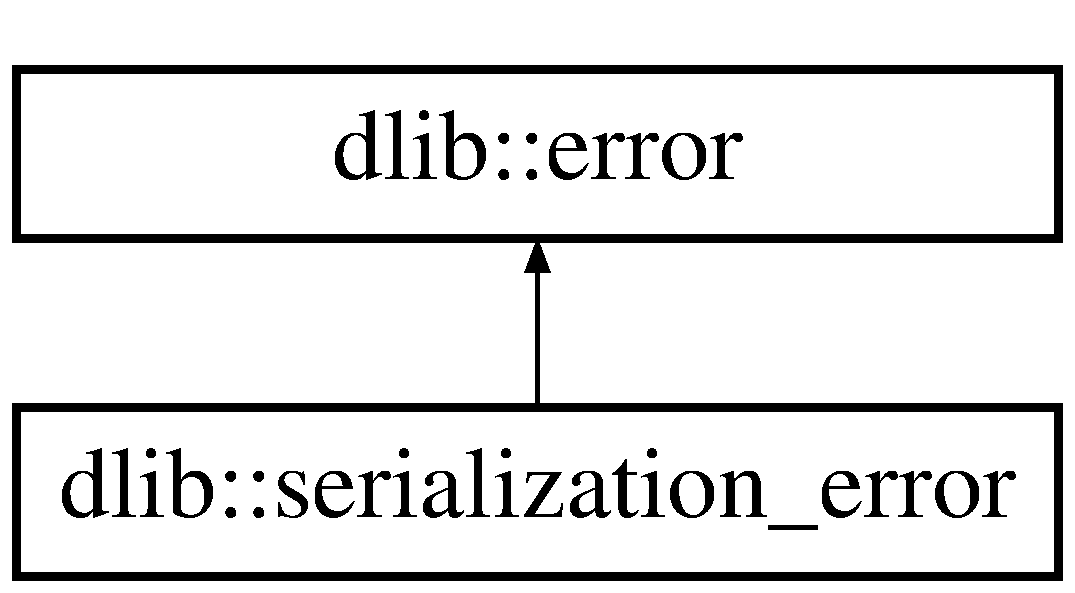
\includegraphics[height=2cm]{classdlib_1_1serialization__error}
\end{center}
\end{figure}
\subsection*{Public Member Functions}
\begin{DoxyCompactItemize}
\item 
\hypertarget{classdlib_1_1serialization__error_aa30f46e6b11a5f0bd530267b5a0a5a6a}{
{\bfseries serialization\_\-error} (const std::string \&e)}
\label{classdlib_1_1serialization__error_aa30f46e6b11a5f0bd530267b5a0a5a6a}

\end{DoxyCompactItemize}


The documentation for this class was generated from the following file:\begin{DoxyCompactItemize}
\item 
source/dlib/serialize.h\end{DoxyCompactItemize}

\hypertarget{classdlib_1_1server}{
\section{dlib::server Class Reference}
\label{classdlib_1_1server}\index{dlib::server@{dlib::server}}
}
\subsection*{Public Types}
\begin{DoxyCompactItemize}
\item 
\hypertarget{classdlib_1_1server_a4bd238e9bf9a8872f9a3f348f7434344}{
typedef server\_\-kernel\_\-1$<$ set\_\-of\_\-cons\_\-1a $>$ {\bfseries kernel\_\-1a}}
\label{classdlib_1_1server_a4bd238e9bf9a8872f9a3f348f7434344}

\item 
\hypertarget{classdlib_1_1server_aa0957a0f980f36596840efa4d0582b94}{
typedef server\_\-kernel\_\-c$<$ kernel\_\-1a $>$ {\bfseries kernel\_\-1a\_\-c}}
\label{classdlib_1_1server_aa0957a0f980f36596840efa4d0582b94}

\item 
\hypertarget{classdlib_1_1server_ab780fb0c4c7bb9fd75c4d817235213fd}{
typedef server\_\-iostream\_\-1$<$ kernel\_\-1a, ssbuf2a, id\_\-map $>$ {\bfseries iostream\_\-1a}}
\label{classdlib_1_1server_ab780fb0c4c7bb9fd75c4d817235213fd}

\item 
\hypertarget{classdlib_1_1server_a8e1ea89df53d40e008a8098eb6ac5e31}{
typedef server\_\-iostream\_\-1$<$ kernel\_\-1a\_\-c, ssbuf2a, id\_\-map $>$ {\bfseries iostream\_\-1a\_\-c}}
\label{classdlib_1_1server_a8e1ea89df53d40e008a8098eb6ac5e31}

\item 
\hypertarget{classdlib_1_1server_a20d7894b5378057da89982af5569f4cb}{
typedef server\_\-http\_\-1$<$ iostream\_\-1a $>$ {\bfseries http\_\-1a}}
\label{classdlib_1_1server_a20d7894b5378057da89982af5569f4cb}

\item 
\hypertarget{classdlib_1_1server_a712ed8cf8587a73ecd05d3386a817ed8}{
typedef server\_\-http\_\-1$<$ iostream\_\-1a\_\-c $>$ {\bfseries http\_\-1a\_\-c}}
\label{classdlib_1_1server_a712ed8cf8587a73ecd05d3386a817ed8}

\end{DoxyCompactItemize}


The documentation for this class was generated from the following file:\begin{DoxyCompactItemize}
\item 
source/dlib/server.h\end{DoxyCompactItemize}

\hypertarget{classdlib_1_1set}{
\section{dlib::set$<$ T, mem\_\-manager, compare $>$ Class Template Reference}
\label{classdlib_1_1set}\index{dlib::set@{dlib::set}}
}
\subsection*{Public Types}
\begin{DoxyCompactItemize}
\item 
\hypertarget{classdlib_1_1set_a9b3e9405436a50324f785cca4b3b5bd5}{
typedef set\_\-kernel\_\-1$<$ T, binary\_\-search\_\-tree\_\-1, mem\_\-manager $>$ {\bfseries kernel\_\-1a}}
\label{classdlib_1_1set_a9b3e9405436a50324f785cca4b3b5bd5}

\item 
\hypertarget{classdlib_1_1set_af046069df11ca98af2f96b613c960f75}{
typedef set\_\-kernel\_\-c$<$ kernel\_\-1a $>$ {\bfseries kernel\_\-1a\_\-c}}
\label{classdlib_1_1set_af046069df11ca98af2f96b613c960f75}

\item 
\hypertarget{classdlib_1_1set_a975fcfac04588a270df8ac81a4bc0357}{
typedef set\_\-kernel\_\-1$<$ T, binary\_\-search\_\-tree\_\-2, mem\_\-manager $>$ {\bfseries kernel\_\-1b}}
\label{classdlib_1_1set_a975fcfac04588a270df8ac81a4bc0357}

\item 
\hypertarget{classdlib_1_1set_abd1f170ff843f4f02cb7526285a3c899}{
typedef set\_\-kernel\_\-c$<$ kernel\_\-1b $>$ {\bfseries kernel\_\-1b\_\-c}}
\label{classdlib_1_1set_abd1f170ff843f4f02cb7526285a3c899}

\item 
\hypertarget{classdlib_1_1set_a2955252a8507df6b9a9592807de1fd25}{
typedef set\_\-compare\_\-1$<$ kernel\_\-1a $>$ {\bfseries compare\_\-1a}}
\label{classdlib_1_1set_a2955252a8507df6b9a9592807de1fd25}

\item 
\hypertarget{classdlib_1_1set_aa03ad6bc042968f5b2e9d47f494e72c2}{
typedef set\_\-compare\_\-1$<$ kernel\_\-1a\_\-c $>$ {\bfseries compare\_\-1a\_\-c}}
\label{classdlib_1_1set_aa03ad6bc042968f5b2e9d47f494e72c2}

\item 
\hypertarget{classdlib_1_1set_ae3b3b08294020e4990c0ec5f78273f34}{
typedef set\_\-compare\_\-1$<$ kernel\_\-1b $>$ {\bfseries compare\_\-1b}}
\label{classdlib_1_1set_ae3b3b08294020e4990c0ec5f78273f34}

\item 
\hypertarget{classdlib_1_1set_ab4a7897c9c2ff109415c5131beee472e}{
typedef set\_\-compare\_\-1$<$ kernel\_\-1b\_\-c $>$ {\bfseries compare\_\-1b\_\-c}}
\label{classdlib_1_1set_ab4a7897c9c2ff109415c5131beee472e}

\end{DoxyCompactItemize}
\subsubsection*{template$<$typename T, typename mem\_\-manager = memory\_\-manager$<$char$>$::kernel\_\-1a, typename compare = std::less$<$T$>$$>$ class dlib::set$<$ T, mem\_\-manager, compare $>$}



The documentation for this class was generated from the following file:\begin{DoxyCompactItemize}
\item 
source/dlib/set.h\end{DoxyCompactItemize}

\hypertarget{classdlib_1_1sliding__buffer}{
\section{dlib::sliding\_\-buffer$<$ T $>$ Class Template Reference}
\label{classdlib_1_1sliding__buffer}\index{dlib::sliding\_\-buffer@{dlib::sliding\_\-buffer}}
}
\subsection*{Public Types}
\begin{DoxyCompactItemize}
\item 
\hypertarget{classdlib_1_1sliding__buffer_ad23f5fcafc7a3c39f633c26f2527a28f}{
typedef sliding\_\-buffer\_\-kernel\_\-1$<$ T $>$ {\bfseries kernel\_\-1a}}
\label{classdlib_1_1sliding__buffer_ad23f5fcafc7a3c39f633c26f2527a28f}

\item 
\hypertarget{classdlib_1_1sliding__buffer_a50f73e9f5f01302aa924d38d622a2701}{
typedef sliding\_\-buffer\_\-kernel\_\-c$<$ kernel\_\-1a $>$ {\bfseries kernel\_\-1a\_\-c}}
\label{classdlib_1_1sliding__buffer_a50f73e9f5f01302aa924d38d622a2701}

\end{DoxyCompactItemize}
\subsubsection*{template$<$typename T$>$ class dlib::sliding\_\-buffer$<$ T $>$}



The documentation for this class was generated from the following file:\begin{DoxyCompactItemize}
\item 
source/dlib/sliding\_\-buffer.h\end{DoxyCompactItemize}

\hypertarget{classdlib_1_1socket__error}{
\section{dlib::socket\_\-error Class Reference}
\label{classdlib_1_1socket__error}\index{dlib::socket\_\-error@{dlib::socket\_\-error}}
}
Inheritance diagram for dlib::socket\_\-error::\begin{figure}[H]
\begin{center}
\leavevmode
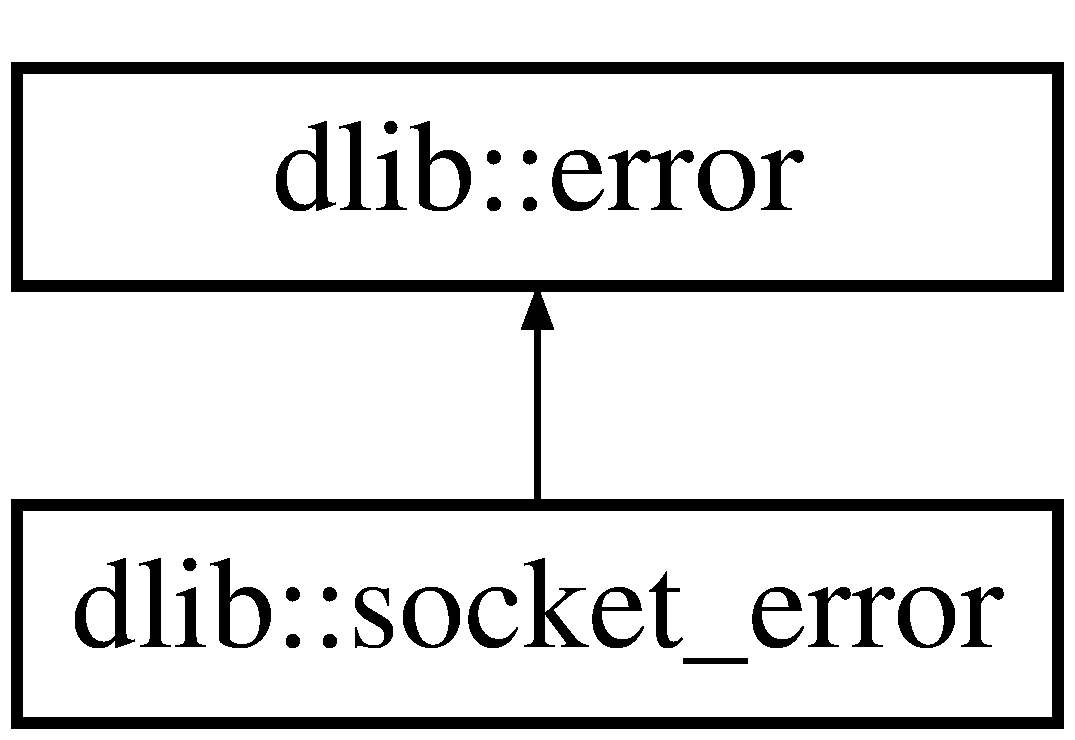
\includegraphics[height=2cm]{classdlib_1_1socket__error}
\end{center}
\end{figure}
\subsection*{Public Member Functions}
\begin{DoxyCompactItemize}
\item 
\hypertarget{classdlib_1_1socket__error_a54067cec0e4569d70cadc1ec33eb9d44}{
{\bfseries socket\_\-error} (error\_\-type t, const std::string \&a)}
\label{classdlib_1_1socket__error_a54067cec0e4569d70cadc1ec33eb9d44}

\item 
\hyperlink{classdlib_1_1socket__error_a0a9b8d66ac787773c3e1d7e19421d6f2}{socket\_\-error} (error\_\-type t)
\item 
\hyperlink{classdlib_1_1socket__error_a894c0c5dbe99a8f6733b875e3913e54a}{socket\_\-error} (const std::string \&a)
\item 
\hyperlink{classdlib_1_1socket__error_a618d1588da7ee235b1d143ce177d5dd8}{socket\_\-error} ()
\end{DoxyCompactItemize}


\subsection{Constructor \& Destructor Documentation}
\hypertarget{classdlib_1_1socket__error_a0a9b8d66ac787773c3e1d7e19421d6f2}{
\index{dlib::socket\_\-error@{dlib::socket\_\-error}!socket\_\-error@{socket\_\-error}}
\index{socket\_\-error@{socket\_\-error}!dlib::socket_error@{dlib::socket\_\-error}}
\subsubsection[{socket\_\-error}]{\setlength{\rightskip}{0pt plus 5cm}dlib::socket\_\-error::socket\_\-error (error\_\-type {\em t})\hspace{0.3cm}{\ttfamily  \mbox{[}inline\mbox{]}}}}
\label{classdlib_1_1socket__error_a0a9b8d66ac787773c3e1d7e19421d6f2}
ensures
\begin{DoxyItemize}
\item type == t
\item info == a ! 
\end{DoxyItemize}\hypertarget{classdlib_1_1socket__error_a894c0c5dbe99a8f6733b875e3913e54a}{
\index{dlib::socket\_\-error@{dlib::socket\_\-error}!socket\_\-error@{socket\_\-error}}
\index{socket\_\-error@{socket\_\-error}!dlib::socket_error@{dlib::socket\_\-error}}
\subsubsection[{socket\_\-error}]{\setlength{\rightskip}{0pt plus 5cm}dlib::socket\_\-error::socket\_\-error (const std::string \& {\em a})\hspace{0.3cm}{\ttfamily  \mbox{[}inline\mbox{]}}}}
\label{classdlib_1_1socket__error_a894c0c5dbe99a8f6733b875e3913e54a}
ensures
\begin{DoxyItemize}
\item type == t
\item info == \char`\"{}\char`\"{} ! 
\end{DoxyItemize}\hypertarget{classdlib_1_1socket__error_a618d1588da7ee235b1d143ce177d5dd8}{
\index{dlib::socket\_\-error@{dlib::socket\_\-error}!socket\_\-error@{socket\_\-error}}
\index{socket\_\-error@{socket\_\-error}!dlib::socket_error@{dlib::socket\_\-error}}
\subsubsection[{socket\_\-error}]{\setlength{\rightskip}{0pt plus 5cm}dlib::socket\_\-error::socket\_\-error ()\hspace{0.3cm}{\ttfamily  \mbox{[}inline\mbox{]}}}}
\label{classdlib_1_1socket__error_a618d1588da7ee235b1d143ce177d5dd8}
ensures
\begin{DoxyItemize}
\item type == ESOCKET
\item info == a ! 
\end{DoxyItemize}

The documentation for this class was generated from the following file:\begin{DoxyCompactItemize}
\item 
source/dlib/error.h\end{DoxyCompactItemize}

\hypertarget{classdlib_1_1sockstreambuf}{
\section{dlib::sockstreambuf Class Reference}
\label{classdlib_1_1sockstreambuf}\index{dlib::sockstreambuf@{dlib::sockstreambuf}}
}
\subsection*{Public Types}
\begin{DoxyCompactItemize}
\item 
\hypertarget{classdlib_1_1sockstreambuf_ac36734b860aee1792252254031511754}{
typedef sockstreambuf\_\-kernel\_\-1 {\bfseries kernel\_\-1a}}
\label{classdlib_1_1sockstreambuf_ac36734b860aee1792252254031511754}

\item 
\hypertarget{classdlib_1_1sockstreambuf_a67192a7a46bb4ef795d401c066b08f44}{
typedef sockstreambuf\_\-kernel\_\-2 {\bfseries kernel\_\-2a}}
\label{classdlib_1_1sockstreambuf_a67192a7a46bb4ef795d401c066b08f44}

\end{DoxyCompactItemize}


The documentation for this class was generated from the following file:\begin{DoxyCompactItemize}
\item 
source/dlib/sockstreambuf.h\end{DoxyCompactItemize}

\hypertarget{classdlib_1_1stack}{
\section{dlib::stack$<$ T, mem\_\-manager $>$ Class Template Reference}
\label{classdlib_1_1stack}\index{dlib::stack@{dlib::stack}}
}
\subsection*{Public Types}
\begin{DoxyCompactItemize}
\item 
\hypertarget{classdlib_1_1stack_a7696878e1040d1639c63d0bfd2b829b2}{
typedef stack\_\-kernel\_\-1$<$ T, mem\_\-manager $>$ {\bfseries kernel\_\-1a}}
\label{classdlib_1_1stack_a7696878e1040d1639c63d0bfd2b829b2}

\item 
\hypertarget{classdlib_1_1stack_a0632f6142cbe703f907a27240f09c248}{
typedef stack\_\-kernel\_\-c$<$ kernel\_\-1a $>$ {\bfseries kernel\_\-1a\_\-c}}
\label{classdlib_1_1stack_a0632f6142cbe703f907a27240f09c248}

\end{DoxyCompactItemize}
\subsubsection*{template$<$typename T, typename mem\_\-manager = memory\_\-manager$<$char$>$::kernel\_\-1a$>$ class dlib::stack$<$ T, mem\_\-manager $>$}



The documentation for this class was generated from the following file:\begin{DoxyCompactItemize}
\item 
source/dlib/stack.h\end{DoxyCompactItemize}

\hypertarget{classdlib_1_1static__map}{
\section{dlib::static\_\-map$<$ domain, range, compare $>$ Class Template Reference}
\label{classdlib_1_1static__map}\index{dlib::static\_\-map@{dlib::static\_\-map}}
}
\subsection*{Public Types}
\begin{DoxyCompactItemize}
\item 
\hypertarget{classdlib_1_1static__map_a8d7cc6df80ef7a0476d9dfa215be09bf}{
typedef static\_\-map\_\-kernel\_\-1$<$ domain, range, compare $>$ {\bfseries kernel\_\-1a}}
\label{classdlib_1_1static__map_a8d7cc6df80ef7a0476d9dfa215be09bf}

\item 
\hypertarget{classdlib_1_1static__map_a5681645ffc274e02120720c00fded24b}{
typedef static\_\-map\_\-kernel\_\-c$<$ kernel\_\-1a $>$ {\bfseries kernel\_\-1a\_\-c}}
\label{classdlib_1_1static__map_a5681645ffc274e02120720c00fded24b}

\end{DoxyCompactItemize}
\subsubsection*{template$<$typename domain, typename range, typename compare = std::less$<$domain$>$$>$ class dlib::static\_\-map$<$ domain, range, compare $>$}



The documentation for this class was generated from the following file:\begin{DoxyCompactItemize}
\item 
source/dlib/static\_\-map.h\end{DoxyCompactItemize}

\hypertarget{classdlib_1_1static__set}{
\section{dlib::static\_\-set$<$ T, compare $>$ Class Template Reference}
\label{classdlib_1_1static__set}\index{dlib::static\_\-set@{dlib::static\_\-set}}
}
\subsection*{Public Types}
\begin{DoxyCompactItemize}
\item 
\hypertarget{classdlib_1_1static__set_a95164c6fadb87feacadfb32f9c2ece36}{
typedef static\_\-set\_\-kernel\_\-1$<$ T, compare $>$ {\bfseries kernel\_\-1a}}
\label{classdlib_1_1static__set_a95164c6fadb87feacadfb32f9c2ece36}

\item 
\hypertarget{classdlib_1_1static__set_afee096146ede621d027a345652a3a0c1}{
typedef static\_\-set\_\-kernel\_\-c$<$ kernel\_\-1a $>$ {\bfseries kernel\_\-1a\_\-c}}
\label{classdlib_1_1static__set_afee096146ede621d027a345652a3a0c1}

\item 
\hypertarget{classdlib_1_1static__set_a285e563d8bd679dbb03f7a382d5405c0}{
typedef static\_\-set\_\-compare\_\-1$<$ kernel\_\-1a $>$ {\bfseries compare\_\-1a}}
\label{classdlib_1_1static__set_a285e563d8bd679dbb03f7a382d5405c0}

\item 
\hypertarget{classdlib_1_1static__set_a72cb14f4eba83913acd9694613ba355d}{
typedef static\_\-set\_\-compare\_\-1$<$ kernel\_\-1a\_\-c $>$ {\bfseries compare\_\-1a\_\-c}}
\label{classdlib_1_1static__set_a72cb14f4eba83913acd9694613ba355d}

\end{DoxyCompactItemize}
\subsubsection*{template$<$typename T, typename compare = std::less$<$T$>$$>$ class dlib::static\_\-set$<$ T, compare $>$}



The documentation for this class was generated from the following file:\begin{DoxyCompactItemize}
\item 
source/dlib/static\_\-set.h\end{DoxyCompactItemize}

\hypertarget{structdlib_1_1static__switch_3_010_00_010_00_010_00_010_00_010_00_010_00_010_00_010_00_010_00_01297db704ac0ccd7cdf569f49ff1837f4}{
\section{dlib::static\_\-switch$<$ 0, 0, 0, 0, 0, 0, 0, 0, 0, 0, 0, 0, 0, 0, 0 $>$ Struct Template Reference}
\label{structdlib_1_1static__switch_3_010_00_010_00_010_00_010_00_010_00_010_00_010_00_010_00_010_00_01297db704ac0ccd7cdf569f49ff1837f4}\index{dlib::static\_\-switch$<$ 0, 0, 0, 0, 0, 0, 0, 0, 0, 0, 0, 0, 0, 0, 0 $>$@{dlib::static\_\-switch$<$ 0, 0, 0, 0, 0, 0, 0, 0, 0, 0, 0, 0, 0, 0, 0 $>$}}
}
\subsection*{Static Public Attributes}
\begin{DoxyCompactItemize}
\item 
\hypertarget{structdlib_1_1static__switch_3_010_00_010_00_010_00_010_00_010_00_010_00_010_00_010_00_010_00_01297db704ac0ccd7cdf569f49ff1837f4_aaa907d7a6b034f114953e0269d53379c}{
static const int {\bfseries value} = 0}
\label{structdlib_1_1static__switch_3_010_00_010_00_010_00_010_00_010_00_010_00_010_00_010_00_010_00_01297db704ac0ccd7cdf569f49ff1837f4_aaa907d7a6b034f114953e0269d53379c}

\end{DoxyCompactItemize}
\subsubsection*{template$<$$>$ struct dlib::static\_\-switch$<$ 0, 0, 0, 0, 0, 0, 0, 0, 0, 0, 0, 0, 0, 0, 0 $>$}



The documentation for this struct was generated from the following file:\begin{DoxyCompactItemize}
\item 
source/dlib/algs.h\end{DoxyCompactItemize}

\hypertarget{structdlib_1_1static__switch_3_010_00_010_00_010_00_010_00_010_00_010_00_010_00_010_00_010_00_0146ef5bf350d722d5ffb766430493f3da}{
\section{dlib::static\_\-switch$<$ 0, 0, 0, 0, 0, 0, 0, 0, 0, 0, 0, 0, 0, 0, 1 $>$ Struct Template Reference}
\label{structdlib_1_1static__switch_3_010_00_010_00_010_00_010_00_010_00_010_00_010_00_010_00_010_00_0146ef5bf350d722d5ffb766430493f3da}\index{dlib::static\_\-switch$<$ 0, 0, 0, 0, 0, 0, 0, 0, 0, 0, 0, 0, 0, 0, 1 $>$@{dlib::static\_\-switch$<$ 0, 0, 0, 0, 0, 0, 0, 0, 0, 0, 0, 0, 0, 0, 1 $>$}}
}
\subsection*{Static Public Attributes}
\begin{DoxyCompactItemize}
\item 
\hypertarget{structdlib_1_1static__switch_3_010_00_010_00_010_00_010_00_010_00_010_00_010_00_010_00_010_00_0146ef5bf350d722d5ffb766430493f3da_ae64db4bea8dac380fcc96e5214165f2b}{
static const int {\bfseries value} = 15}
\label{structdlib_1_1static__switch_3_010_00_010_00_010_00_010_00_010_00_010_00_010_00_010_00_010_00_0146ef5bf350d722d5ffb766430493f3da_ae64db4bea8dac380fcc96e5214165f2b}

\end{DoxyCompactItemize}
\subsubsection*{template$<$$>$ struct dlib::static\_\-switch$<$ 0, 0, 0, 0, 0, 0, 0, 0, 0, 0, 0, 0, 0, 0, 1 $>$}



The documentation for this struct was generated from the following file:\begin{DoxyCompactItemize}
\item 
source/dlib/algs.h\end{DoxyCompactItemize}

\hypertarget{structdlib_1_1static__switch_3_010_00_010_00_010_00_010_00_010_00_010_00_010_00_010_00_010_00_016cef4822784544663fb033f63ec96728}{
\section{dlib::static\_\-switch$<$ 0, 0, 0, 0, 0, 0, 0, 0, 0, 0, 0, 0, 0, 1, 0 $>$ Struct Template Reference}
\label{structdlib_1_1static__switch_3_010_00_010_00_010_00_010_00_010_00_010_00_010_00_010_00_010_00_016cef4822784544663fb033f63ec96728}\index{dlib::static\_\-switch$<$ 0, 0, 0, 0, 0, 0, 0, 0, 0, 0, 0, 0, 0, 1, 0 $>$@{dlib::static\_\-switch$<$ 0, 0, 0, 0, 0, 0, 0, 0, 0, 0, 0, 0, 0, 1, 0 $>$}}
}
\subsection*{Static Public Attributes}
\begin{DoxyCompactItemize}
\item 
\hypertarget{structdlib_1_1static__switch_3_010_00_010_00_010_00_010_00_010_00_010_00_010_00_010_00_010_00_016cef4822784544663fb033f63ec96728_af4791171a90f6cf2f3f5db2907418ea1}{
static const int {\bfseries value} = 14}
\label{structdlib_1_1static__switch_3_010_00_010_00_010_00_010_00_010_00_010_00_010_00_010_00_010_00_016cef4822784544663fb033f63ec96728_af4791171a90f6cf2f3f5db2907418ea1}

\end{DoxyCompactItemize}
\subsubsection*{template$<$$>$ struct dlib::static\_\-switch$<$ 0, 0, 0, 0, 0, 0, 0, 0, 0, 0, 0, 0, 0, 1, 0 $>$}



The documentation for this struct was generated from the following file:\begin{DoxyCompactItemize}
\item 
source/dlib/algs.h\end{DoxyCompactItemize}

\hypertarget{structdlib_1_1static__switch_3_010_00_010_00_010_00_010_00_010_00_010_00_010_00_010_00_010_00_01de46d05550779d2bbe7720ab7bfdb3cc}{
\section{dlib::static\_\-switch$<$ 0, 0, 0, 0, 0, 0, 0, 0, 0, 0, 0, 0, 1, 0, 0 $>$ Struct Template Reference}
\label{structdlib_1_1static__switch_3_010_00_010_00_010_00_010_00_010_00_010_00_010_00_010_00_010_00_01de46d05550779d2bbe7720ab7bfdb3cc}\index{dlib::static\_\-switch$<$ 0, 0, 0, 0, 0, 0, 0, 0, 0, 0, 0, 0, 1, 0, 0 $>$@{dlib::static\_\-switch$<$ 0, 0, 0, 0, 0, 0, 0, 0, 0, 0, 0, 0, 1, 0, 0 $>$}}
}
\subsection*{Static Public Attributes}
\begin{DoxyCompactItemize}
\item 
\hypertarget{structdlib_1_1static__switch_3_010_00_010_00_010_00_010_00_010_00_010_00_010_00_010_00_010_00_01de46d05550779d2bbe7720ab7bfdb3cc_a0c184f8ebdf3aa4afb71b6df3e17c353}{
static const int {\bfseries value} = 13}
\label{structdlib_1_1static__switch_3_010_00_010_00_010_00_010_00_010_00_010_00_010_00_010_00_010_00_01de46d05550779d2bbe7720ab7bfdb3cc_a0c184f8ebdf3aa4afb71b6df3e17c353}

\end{DoxyCompactItemize}
\subsubsection*{template$<$$>$ struct dlib::static\_\-switch$<$ 0, 0, 0, 0, 0, 0, 0, 0, 0, 0, 0, 0, 1, 0, 0 $>$}



The documentation for this struct was generated from the following file:\begin{DoxyCompactItemize}
\item 
source/dlib/algs.h\end{DoxyCompactItemize}

\hypertarget{structdlib_1_1static__switch_3_010_00_010_00_010_00_010_00_010_00_010_00_010_00_010_00_010_00_0147e6a475a446e40bfc581407a8174f9f}{
\section{dlib::static\_\-switch$<$ 0, 0, 0, 0, 0, 0, 0, 0, 0, 0, 0, 1, 0, 0, 0 $>$ Struct Template Reference}
\label{structdlib_1_1static__switch_3_010_00_010_00_010_00_010_00_010_00_010_00_010_00_010_00_010_00_0147e6a475a446e40bfc581407a8174f9f}\index{dlib::static\_\-switch$<$ 0, 0, 0, 0, 0, 0, 0, 0, 0, 0, 0, 1, 0, 0, 0 $>$@{dlib::static\_\-switch$<$ 0, 0, 0, 0, 0, 0, 0, 0, 0, 0, 0, 1, 0, 0, 0 $>$}}
}
\subsection*{Static Public Attributes}
\begin{DoxyCompactItemize}
\item 
\hypertarget{structdlib_1_1static__switch_3_010_00_010_00_010_00_010_00_010_00_010_00_010_00_010_00_010_00_0147e6a475a446e40bfc581407a8174f9f_a6d9fe6baa2a0bce3e63e8e05806d9837}{
static const int {\bfseries value} = 12}
\label{structdlib_1_1static__switch_3_010_00_010_00_010_00_010_00_010_00_010_00_010_00_010_00_010_00_0147e6a475a446e40bfc581407a8174f9f_a6d9fe6baa2a0bce3e63e8e05806d9837}

\end{DoxyCompactItemize}
\subsubsection*{template$<$$>$ struct dlib::static\_\-switch$<$ 0, 0, 0, 0, 0, 0, 0, 0, 0, 0, 0, 1, 0, 0, 0 $>$}



The documentation for this struct was generated from the following file:\begin{DoxyCompactItemize}
\item 
source/dlib/algs.h\end{DoxyCompactItemize}

\hypertarget{structdlib_1_1static__switch_3_010_00_010_00_010_00_010_00_010_00_010_00_010_00_010_00_010_00_0145cbcc58af0c0409c47cc48fc11394ec}{
\section{dlib::static\_\-switch$<$ 0, 0, 0, 0, 0, 0, 0, 0, 0, 0, 1, 0, 0, 0, 0 $>$ Struct Template Reference}
\label{structdlib_1_1static__switch_3_010_00_010_00_010_00_010_00_010_00_010_00_010_00_010_00_010_00_0145cbcc58af0c0409c47cc48fc11394ec}\index{dlib::static\_\-switch$<$ 0, 0, 0, 0, 0, 0, 0, 0, 0, 0, 1, 0, 0, 0, 0 $>$@{dlib::static\_\-switch$<$ 0, 0, 0, 0, 0, 0, 0, 0, 0, 0, 1, 0, 0, 0, 0 $>$}}
}
\subsection*{Static Public Attributes}
\begin{DoxyCompactItemize}
\item 
\hypertarget{structdlib_1_1static__switch_3_010_00_010_00_010_00_010_00_010_00_010_00_010_00_010_00_010_00_0145cbcc58af0c0409c47cc48fc11394ec_a2553c31a2b94169adbbb842919989879}{
static const int {\bfseries value} = 11}
\label{structdlib_1_1static__switch_3_010_00_010_00_010_00_010_00_010_00_010_00_010_00_010_00_010_00_0145cbcc58af0c0409c47cc48fc11394ec_a2553c31a2b94169adbbb842919989879}

\end{DoxyCompactItemize}
\subsubsection*{template$<$$>$ struct dlib::static\_\-switch$<$ 0, 0, 0, 0, 0, 0, 0, 0, 0, 0, 1, 0, 0, 0, 0 $>$}



The documentation for this struct was generated from the following file:\begin{DoxyCompactItemize}
\item 
source/dlib/algs.h\end{DoxyCompactItemize}

\hypertarget{structdlib_1_1static__switch_3_010_00_010_00_010_00_010_00_010_00_010_00_010_00_010_00_010_00_011e8c10a795cabaf3f5d590d7d2ed509c}{
\section{dlib::static\_\-switch$<$ 0, 0, 0, 0, 0, 0, 0, 0, 0, 1, 0, 0, 0, 0, 0 $>$ Struct Template Reference}
\label{structdlib_1_1static__switch_3_010_00_010_00_010_00_010_00_010_00_010_00_010_00_010_00_010_00_011e8c10a795cabaf3f5d590d7d2ed509c}\index{dlib::static\_\-switch$<$ 0, 0, 0, 0, 0, 0, 0, 0, 0, 1, 0, 0, 0, 0, 0 $>$@{dlib::static\_\-switch$<$ 0, 0, 0, 0, 0, 0, 0, 0, 0, 1, 0, 0, 0, 0, 0 $>$}}
}
\subsection*{Static Public Attributes}
\begin{DoxyCompactItemize}
\item 
\hypertarget{structdlib_1_1static__switch_3_010_00_010_00_010_00_010_00_010_00_010_00_010_00_010_00_010_00_011e8c10a795cabaf3f5d590d7d2ed509c_a391ff2a5c1e86a76962e16163ef7deff}{
static const int {\bfseries value} = 10}
\label{structdlib_1_1static__switch_3_010_00_010_00_010_00_010_00_010_00_010_00_010_00_010_00_010_00_011e8c10a795cabaf3f5d590d7d2ed509c_a391ff2a5c1e86a76962e16163ef7deff}

\end{DoxyCompactItemize}
\subsubsection*{template$<$$>$ struct dlib::static\_\-switch$<$ 0, 0, 0, 0, 0, 0, 0, 0, 0, 1, 0, 0, 0, 0, 0 $>$}



The documentation for this struct was generated from the following file:\begin{DoxyCompactItemize}
\item 
source/dlib/algs.h\end{DoxyCompactItemize}

\hypertarget{structdlib_1_1static__switch_3_010_00_010_00_010_00_010_00_010_00_010_00_010_00_010_00_011_00_010dd8c605dbfd043e236f91723a992215}{
\section{dlib::static\_\-switch$<$ 0, 0, 0, 0, 0, 0, 0, 0, 1, 0, 0, 0, 0, 0, 0 $>$ Struct Template Reference}
\label{structdlib_1_1static__switch_3_010_00_010_00_010_00_010_00_010_00_010_00_010_00_010_00_011_00_010dd8c605dbfd043e236f91723a992215}\index{dlib::static\_\-switch$<$ 0, 0, 0, 0, 0, 0, 0, 0, 1, 0, 0, 0, 0, 0, 0 $>$@{dlib::static\_\-switch$<$ 0, 0, 0, 0, 0, 0, 0, 0, 1, 0, 0, 0, 0, 0, 0 $>$}}
}
\subsection*{Static Public Attributes}
\begin{DoxyCompactItemize}
\item 
\hypertarget{structdlib_1_1static__switch_3_010_00_010_00_010_00_010_00_010_00_010_00_010_00_010_00_011_00_010dd8c605dbfd043e236f91723a992215_a74c6ec197f7f540d8e941594e9848e74}{
static const int {\bfseries value} = 9}
\label{structdlib_1_1static__switch_3_010_00_010_00_010_00_010_00_010_00_010_00_010_00_010_00_011_00_010dd8c605dbfd043e236f91723a992215_a74c6ec197f7f540d8e941594e9848e74}

\end{DoxyCompactItemize}
\subsubsection*{template$<$$>$ struct dlib::static\_\-switch$<$ 0, 0, 0, 0, 0, 0, 0, 0, 1, 0, 0, 0, 0, 0, 0 $>$}



The documentation for this struct was generated from the following file:\begin{DoxyCompactItemize}
\item 
source/dlib/algs.h\end{DoxyCompactItemize}

\hypertarget{structdlib_1_1static__switch_3_010_00_010_00_010_00_010_00_010_00_010_00_010_00_011_00_010_00_0105236f4c56e9666de491dbb566b29360}{
\section{dlib::static\_\-switch$<$ 0, 0, 0, 0, 0, 0, 0, 1, 0, 0, 0, 0, 0, 0, 0 $>$ Struct Template Reference}
\label{structdlib_1_1static__switch_3_010_00_010_00_010_00_010_00_010_00_010_00_010_00_011_00_010_00_0105236f4c56e9666de491dbb566b29360}\index{dlib::static\_\-switch$<$ 0, 0, 0, 0, 0, 0, 0, 1, 0, 0, 0, 0, 0, 0, 0 $>$@{dlib::static\_\-switch$<$ 0, 0, 0, 0, 0, 0, 0, 1, 0, 0, 0, 0, 0, 0, 0 $>$}}
}
\subsection*{Static Public Attributes}
\begin{DoxyCompactItemize}
\item 
\hypertarget{structdlib_1_1static__switch_3_010_00_010_00_010_00_010_00_010_00_010_00_010_00_011_00_010_00_0105236f4c56e9666de491dbb566b29360_a8571742226340f5a4be6eca0bf104f94}{
static const int {\bfseries value} = 8}
\label{structdlib_1_1static__switch_3_010_00_010_00_010_00_010_00_010_00_010_00_010_00_011_00_010_00_0105236f4c56e9666de491dbb566b29360_a8571742226340f5a4be6eca0bf104f94}

\end{DoxyCompactItemize}
\subsubsection*{template$<$$>$ struct dlib::static\_\-switch$<$ 0, 0, 0, 0, 0, 0, 0, 1, 0, 0, 0, 0, 0, 0, 0 $>$}



The documentation for this struct was generated from the following file:\begin{DoxyCompactItemize}
\item 
source/dlib/algs.h\end{DoxyCompactItemize}

\hypertarget{structdlib_1_1static__switch_3_010_00_010_00_010_00_010_00_010_00_010_00_011_00_010_00_010_00_01f96a27221d42a17b5e8ff3b09c0ae4ae}{
\section{dlib::static\_\-switch$<$ 0, 0, 0, 0, 0, 0, 1, 0, 0, 0, 0, 0, 0, 0, 0 $>$ Struct Template Reference}
\label{structdlib_1_1static__switch_3_010_00_010_00_010_00_010_00_010_00_010_00_011_00_010_00_010_00_01f96a27221d42a17b5e8ff3b09c0ae4ae}\index{dlib::static\_\-switch$<$ 0, 0, 0, 0, 0, 0, 1, 0, 0, 0, 0, 0, 0, 0, 0 $>$@{dlib::static\_\-switch$<$ 0, 0, 0, 0, 0, 0, 1, 0, 0, 0, 0, 0, 0, 0, 0 $>$}}
}
\subsection*{Static Public Attributes}
\begin{DoxyCompactItemize}
\item 
\hypertarget{structdlib_1_1static__switch_3_010_00_010_00_010_00_010_00_010_00_010_00_011_00_010_00_010_00_01f96a27221d42a17b5e8ff3b09c0ae4ae_a80b00d374ef0dcd6b4b750dae750723a}{
static const int {\bfseries value} = 7}
\label{structdlib_1_1static__switch_3_010_00_010_00_010_00_010_00_010_00_010_00_011_00_010_00_010_00_01f96a27221d42a17b5e8ff3b09c0ae4ae_a80b00d374ef0dcd6b4b750dae750723a}

\end{DoxyCompactItemize}
\subsubsection*{template$<$$>$ struct dlib::static\_\-switch$<$ 0, 0, 0, 0, 0, 0, 1, 0, 0, 0, 0, 0, 0, 0, 0 $>$}



The documentation for this struct was generated from the following file:\begin{DoxyCompactItemize}
\item 
source/dlib/algs.h\end{DoxyCompactItemize}

\hypertarget{structdlib_1_1static__switch_3_010_00_010_00_010_00_010_00_010_00_011_00_010_00_010_00_010_00_01065a8f5a38c76e0fbec03f2ecf64307a}{
\section{dlib::static\_\-switch$<$ 0, 0, 0, 0, 0, 1, 0, 0, 0, 0, 0, 0, 0, 0, 0 $>$ Struct Template Reference}
\label{structdlib_1_1static__switch_3_010_00_010_00_010_00_010_00_010_00_011_00_010_00_010_00_010_00_01065a8f5a38c76e0fbec03f2ecf64307a}\index{dlib::static\_\-switch$<$ 0, 0, 0, 0, 0, 1, 0, 0, 0, 0, 0, 0, 0, 0, 0 $>$@{dlib::static\_\-switch$<$ 0, 0, 0, 0, 0, 1, 0, 0, 0, 0, 0, 0, 0, 0, 0 $>$}}
}
\subsection*{Static Public Attributes}
\begin{DoxyCompactItemize}
\item 
\hypertarget{structdlib_1_1static__switch_3_010_00_010_00_010_00_010_00_010_00_011_00_010_00_010_00_010_00_01065a8f5a38c76e0fbec03f2ecf64307a_a2fb2a8c6459dda970b89f8160d7bf589}{
static const int {\bfseries value} = 6}
\label{structdlib_1_1static__switch_3_010_00_010_00_010_00_010_00_010_00_011_00_010_00_010_00_010_00_01065a8f5a38c76e0fbec03f2ecf64307a_a2fb2a8c6459dda970b89f8160d7bf589}

\end{DoxyCompactItemize}
\subsubsection*{template$<$$>$ struct dlib::static\_\-switch$<$ 0, 0, 0, 0, 0, 1, 0, 0, 0, 0, 0, 0, 0, 0, 0 $>$}



The documentation for this struct was generated from the following file:\begin{DoxyCompactItemize}
\item 
source/dlib/algs.h\end{DoxyCompactItemize}

\hypertarget{structdlib_1_1static__switch_3_010_00_010_00_010_00_010_00_011_00_010_00_010_00_010_00_010_00_01ff4b50cffbfc7efeb2ebcd8ac49664ca}{
\section{dlib::static\_\-switch$<$ 0, 0, 0, 0, 1, 0, 0, 0, 0, 0, 0, 0, 0, 0, 0 $>$ Struct Template Reference}
\label{structdlib_1_1static__switch_3_010_00_010_00_010_00_010_00_011_00_010_00_010_00_010_00_010_00_01ff4b50cffbfc7efeb2ebcd8ac49664ca}\index{dlib::static\_\-switch$<$ 0, 0, 0, 0, 1, 0, 0, 0, 0, 0, 0, 0, 0, 0, 0 $>$@{dlib::static\_\-switch$<$ 0, 0, 0, 0, 1, 0, 0, 0, 0, 0, 0, 0, 0, 0, 0 $>$}}
}
\subsection*{Static Public Attributes}
\begin{DoxyCompactItemize}
\item 
\hypertarget{structdlib_1_1static__switch_3_010_00_010_00_010_00_010_00_011_00_010_00_010_00_010_00_010_00_01ff4b50cffbfc7efeb2ebcd8ac49664ca_adce77c801132c83207d4c40b795a3bad}{
static const int {\bfseries value} = 5}
\label{structdlib_1_1static__switch_3_010_00_010_00_010_00_010_00_011_00_010_00_010_00_010_00_010_00_01ff4b50cffbfc7efeb2ebcd8ac49664ca_adce77c801132c83207d4c40b795a3bad}

\end{DoxyCompactItemize}
\subsubsection*{template$<$$>$ struct dlib::static\_\-switch$<$ 0, 0, 0, 0, 1, 0, 0, 0, 0, 0, 0, 0, 0, 0, 0 $>$}



The documentation for this struct was generated from the following file:\begin{DoxyCompactItemize}
\item 
source/dlib/algs.h\end{DoxyCompactItemize}

\hypertarget{structdlib_1_1static__switch_3_010_00_010_00_010_00_011_00_010_00_010_00_010_00_010_00_010_00_017e7e1ea6f90a3743d68a10bc9ac43767}{
\section{dlib::static\_\-switch$<$ 0, 0, 0, 1, 0, 0, 0, 0, 0, 0, 0, 0, 0, 0, 0 $>$ Struct Template Reference}
\label{structdlib_1_1static__switch_3_010_00_010_00_010_00_011_00_010_00_010_00_010_00_010_00_010_00_017e7e1ea6f90a3743d68a10bc9ac43767}\index{dlib::static\_\-switch$<$ 0, 0, 0, 1, 0, 0, 0, 0, 0, 0, 0, 0, 0, 0, 0 $>$@{dlib::static\_\-switch$<$ 0, 0, 0, 1, 0, 0, 0, 0, 0, 0, 0, 0, 0, 0, 0 $>$}}
}
\subsection*{Static Public Attributes}
\begin{DoxyCompactItemize}
\item 
\hypertarget{structdlib_1_1static__switch_3_010_00_010_00_010_00_011_00_010_00_010_00_010_00_010_00_010_00_017e7e1ea6f90a3743d68a10bc9ac43767_ad2f9fc307a9e7fbd1ac4b1a9f1f28e85}{
static const int {\bfseries value} = 4}
\label{structdlib_1_1static__switch_3_010_00_010_00_010_00_011_00_010_00_010_00_010_00_010_00_010_00_017e7e1ea6f90a3743d68a10bc9ac43767_ad2f9fc307a9e7fbd1ac4b1a9f1f28e85}

\end{DoxyCompactItemize}
\subsubsection*{template$<$$>$ struct dlib::static\_\-switch$<$ 0, 0, 0, 1, 0, 0, 0, 0, 0, 0, 0, 0, 0, 0, 0 $>$}



The documentation for this struct was generated from the following file:\begin{DoxyCompactItemize}
\item 
source/dlib/algs.h\end{DoxyCompactItemize}

\hypertarget{structdlib_1_1static__switch_3_010_00_010_00_011_00_010_00_010_00_010_00_010_00_010_00_010_00_01f20039fe97478cfcdfb8a6fb10d88c23}{
\section{dlib::static\_\-switch$<$ 0, 0, 1, 0, 0, 0, 0, 0, 0, 0, 0, 0, 0, 0, 0 $>$ Struct Template Reference}
\label{structdlib_1_1static__switch_3_010_00_010_00_011_00_010_00_010_00_010_00_010_00_010_00_010_00_01f20039fe97478cfcdfb8a6fb10d88c23}\index{dlib::static\_\-switch$<$ 0, 0, 1, 0, 0, 0, 0, 0, 0, 0, 0, 0, 0, 0, 0 $>$@{dlib::static\_\-switch$<$ 0, 0, 1, 0, 0, 0, 0, 0, 0, 0, 0, 0, 0, 0, 0 $>$}}
}
\subsection*{Static Public Attributes}
\begin{DoxyCompactItemize}
\item 
\hypertarget{structdlib_1_1static__switch_3_010_00_010_00_011_00_010_00_010_00_010_00_010_00_010_00_010_00_01f20039fe97478cfcdfb8a6fb10d88c23_a1fc5d4f9f68e19ee7b9b03e3f6abd412}{
static const int {\bfseries value} = 3}
\label{structdlib_1_1static__switch_3_010_00_010_00_011_00_010_00_010_00_010_00_010_00_010_00_010_00_01f20039fe97478cfcdfb8a6fb10d88c23_a1fc5d4f9f68e19ee7b9b03e3f6abd412}

\end{DoxyCompactItemize}
\subsubsection*{template$<$$>$ struct dlib::static\_\-switch$<$ 0, 0, 1, 0, 0, 0, 0, 0, 0, 0, 0, 0, 0, 0, 0 $>$}



The documentation for this struct was generated from the following file:\begin{DoxyCompactItemize}
\item 
source/dlib/algs.h\end{DoxyCompactItemize}

\hypertarget{structdlib_1_1static__switch_3_010_00_011_00_010_00_010_00_010_00_010_00_010_00_010_00_010_00_013c4ac657bc48737c62a5b545ecf666e2}{
\section{dlib::static\_\-switch$<$ 0, 1, 0, 0, 0, 0, 0, 0, 0, 0, 0, 0, 0, 0, 0 $>$ Struct Template Reference}
\label{structdlib_1_1static__switch_3_010_00_011_00_010_00_010_00_010_00_010_00_010_00_010_00_010_00_013c4ac657bc48737c62a5b545ecf666e2}\index{dlib::static\_\-switch$<$ 0, 1, 0, 0, 0, 0, 0, 0, 0, 0, 0, 0, 0, 0, 0 $>$@{dlib::static\_\-switch$<$ 0, 1, 0, 0, 0, 0, 0, 0, 0, 0, 0, 0, 0, 0, 0 $>$}}
}
\subsection*{Static Public Attributes}
\begin{DoxyCompactItemize}
\item 
\hypertarget{structdlib_1_1static__switch_3_010_00_011_00_010_00_010_00_010_00_010_00_010_00_010_00_010_00_013c4ac657bc48737c62a5b545ecf666e2_a65d209ffff95f58e8b31fa66f53ab375}{
static const int {\bfseries value} = 2}
\label{structdlib_1_1static__switch_3_010_00_011_00_010_00_010_00_010_00_010_00_010_00_010_00_010_00_013c4ac657bc48737c62a5b545ecf666e2_a65d209ffff95f58e8b31fa66f53ab375}

\end{DoxyCompactItemize}
\subsubsection*{template$<$$>$ struct dlib::static\_\-switch$<$ 0, 1, 0, 0, 0, 0, 0, 0, 0, 0, 0, 0, 0, 0, 0 $>$}



The documentation for this struct was generated from the following file:\begin{DoxyCompactItemize}
\item 
source/dlib/algs.h\end{DoxyCompactItemize}

\hypertarget{structdlib_1_1static__switch_3_011_00_010_00_010_00_010_00_010_00_010_00_010_00_010_00_010_00_01e6d4ee9dd0db82c25ad3e5e162ffcf57}{
\section{dlib::static\_\-switch$<$ 1, 0, 0, 0, 0, 0, 0, 0, 0, 0, 0, 0, 0, 0, 0 $>$ Struct Template Reference}
\label{structdlib_1_1static__switch_3_011_00_010_00_010_00_010_00_010_00_010_00_010_00_010_00_010_00_01e6d4ee9dd0db82c25ad3e5e162ffcf57}\index{dlib::static\_\-switch$<$ 1, 0, 0, 0, 0, 0, 0, 0, 0, 0, 0, 0, 0, 0, 0 $>$@{dlib::static\_\-switch$<$ 1, 0, 0, 0, 0, 0, 0, 0, 0, 0, 0, 0, 0, 0, 0 $>$}}
}
\subsection*{Static Public Attributes}
\begin{DoxyCompactItemize}
\item 
\hypertarget{structdlib_1_1static__switch_3_011_00_010_00_010_00_010_00_010_00_010_00_010_00_010_00_010_00_01e6d4ee9dd0db82c25ad3e5e162ffcf57_aac2f646850953922ab9403d67f23005f}{
static const int {\bfseries value} = 1}
\label{structdlib_1_1static__switch_3_011_00_010_00_010_00_010_00_010_00_010_00_010_00_010_00_010_00_01e6d4ee9dd0db82c25ad3e5e162ffcf57_aac2f646850953922ab9403d67f23005f}

\end{DoxyCompactItemize}
\subsubsection*{template$<$$>$ struct dlib::static\_\-switch$<$ 1, 0, 0, 0, 0, 0, 0, 0, 0, 0, 0, 0, 0, 0, 0 $>$}



The documentation for this struct was generated from the following file:\begin{DoxyCompactItemize}
\item 
source/dlib/algs.h\end{DoxyCompactItemize}

\hypertarget{structdlib_1_1std__alloc__compare}{
\section{dlib::std\_\-alloc\_\-compare$<$ M1, M2, enabled $>$ Struct Template Reference}
\label{structdlib_1_1std__alloc__compare}\index{dlib::std\_\-alloc\_\-compare@{dlib::std\_\-alloc\_\-compare}}
}
\subsection*{Static Public Attributes}
\begin{DoxyCompactItemize}
\item 
\hypertarget{structdlib_1_1std__alloc__compare_ad2777c57afe1b1f76238bf8e8c5916fa}{
static const bool {\bfseries are\_\-interchangeable} = false}
\label{structdlib_1_1std__alloc__compare_ad2777c57afe1b1f76238bf8e8c5916fa}

\end{DoxyCompactItemize}
\subsubsection*{template$<$typename M1, typename M2, typename enabled = void$>$ struct dlib::std\_\-alloc\_\-compare$<$ M1, M2, enabled $>$}



The documentation for this struct was generated from the following file:\begin{DoxyCompactItemize}
\item 
source/dlib/std\_\-allocator.h\end{DoxyCompactItemize}

\hypertarget{structdlib_1_1std__alloc__compare_3_01M_00_01M_00_01typename_01enable__if__c_3_01M_1_1is__stateless_01_4_1_1type_01_4}{
\section{dlib::std\_\-alloc\_\-compare$<$ M, M, typename enable\_\-if\_\-c$<$ M::is\_\-stateless $>$::type $>$ Struct Template Reference}
\label{structdlib_1_1std__alloc__compare_3_01M_00_01M_00_01typename_01enable__if__c_3_01M_1_1is__stateless_01_4_1_1type_01_4}\index{dlib::std\_\-alloc\_\-compare$<$ M, M, typename enable\_\-if\_\-c$<$ M::is\_\-stateless $>$::type $>$@{dlib::std\_\-alloc\_\-compare$<$ M, M, typename enable\_\-if\_\-c$<$ M::is\_\-stateless $>$::type $>$}}
}
\subsection*{Static Public Attributes}
\begin{DoxyCompactItemize}
\item 
\hypertarget{structdlib_1_1std__alloc__compare_3_01M_00_01M_00_01typename_01enable__if__c_3_01M_1_1is__stateless_01_4_1_1type_01_4_aea50547f254a5fff23948f8fdfdae0b0}{
static const bool {\bfseries are\_\-interchangeable} = true}
\label{structdlib_1_1std__alloc__compare_3_01M_00_01M_00_01typename_01enable__if__c_3_01M_1_1is__stateless_01_4_1_1type_01_4_aea50547f254a5fff23948f8fdfdae0b0}

\end{DoxyCompactItemize}
\subsubsection*{template$<$typename M$>$ struct dlib::std\_\-alloc\_\-compare$<$ M, M, typename enable\_\-if\_\-c$<$ M::is\_\-stateless $>$::type $>$}



The documentation for this struct was generated from the following file:\begin{DoxyCompactItemize}
\item 
source/dlib/std\_\-allocator.h\end{DoxyCompactItemize}

\hypertarget{structdlib_1_1std__alloc__compare_3_01M1_00_01M2_00_01typename_01enable__if_3_01is__same__type_3982ed367adf685c0833f1e72cac3711f}{
\section{dlib::std\_\-alloc\_\-compare$<$ M1, M2, typename enable\_\-if$<$ is\_\-same\_\-type$<$ typename M1::mm\_\-global\_\-type, typename M2::mm\_\-global\_\-type $>$ $>$::type $>$ Struct Template Reference}
\label{structdlib_1_1std__alloc__compare_3_01M1_00_01M2_00_01typename_01enable__if_3_01is__same__type_3982ed367adf685c0833f1e72cac3711f}\index{dlib::std\_\-alloc\_\-compare$<$ M1, M2, typename enable\_\-if$<$ is\_\-same\_\-type$<$ typename M1::mm\_\-global\_\-type, typename M2::mm\_\-global\_\-type $>$ $>$::type $>$@{dlib::std\_\-alloc\_\-compare$<$ M1, M2, typename enable\_\-if$<$ is\_\-same\_\-type$<$ typename M1::mm\_\-global\_\-type, typename M2::mm\_\-global\_\-type $>$ $>$::type $>$}}
}
\subsection*{Static Public Attributes}
\begin{DoxyCompactItemize}
\item 
\hypertarget{structdlib_1_1std__alloc__compare_3_01M1_00_01M2_00_01typename_01enable__if_3_01is__same__type_3982ed367adf685c0833f1e72cac3711f_acb2160f9ae7aea0af12b5c62ea3ed897}{
static const bool {\bfseries are\_\-interchangeable} = true}
\label{structdlib_1_1std__alloc__compare_3_01M1_00_01M2_00_01typename_01enable__if_3_01is__same__type_3982ed367adf685c0833f1e72cac3711f_acb2160f9ae7aea0af12b5c62ea3ed897}

\end{DoxyCompactItemize}
\subsubsection*{template$<$typename M1, typename M2$>$ struct dlib::std\_\-alloc\_\-compare$<$ M1, M2, typename enable\_\-if$<$ is\_\-same\_\-type$<$ typename M1::mm\_\-global\_\-type, typename M2::mm\_\-global\_\-type $>$ $>$::type $>$}



The documentation for this struct was generated from the following file:\begin{DoxyCompactItemize}
\item 
source/dlib/std\_\-allocator.h\end{DoxyCompactItemize}

\hypertarget{classdlib_1_1std__allocator}{
\section{dlib::std\_\-allocator$<$ T, M $>$ Class Template Reference}
\label{classdlib_1_1std__allocator}\index{dlib::std\_\-allocator@{dlib::std\_\-allocator}}
}
\subsection*{Classes}
\begin{DoxyCompactItemize}
\item 
struct \hyperlink{structdlib_1_1std__allocator_1_1rebind}{rebind}
\end{DoxyCompactItemize}
\subsection*{Public Types}
\begin{DoxyCompactItemize}
\item 
typedef std::size\_\-t \hyperlink{classdlib_1_1std__allocator_afbdfb9dc5c127fd82f2b1c9f3b1989bf}{size\_\-type}
\item 
\hypertarget{classdlib_1_1std__allocator_aedfcf400c07fda90dd1902c6aba1a25a}{
typedef std::ptrdiff\_\-t {\bfseries difference\_\-type}}
\label{classdlib_1_1std__allocator_aedfcf400c07fda90dd1902c6aba1a25a}

\item 
\hypertarget{classdlib_1_1std__allocator_aa7c4dca5117b25c5f6983cf9ac871b47}{
typedef T $\ast$ {\bfseries pointer}}
\label{classdlib_1_1std__allocator_aa7c4dca5117b25c5f6983cf9ac871b47}

\item 
\hypertarget{classdlib_1_1std__allocator_acfe99966877caf2e39e1164eb6610c1e}{
typedef const T $\ast$ {\bfseries const\_\-pointer}}
\label{classdlib_1_1std__allocator_acfe99966877caf2e39e1164eb6610c1e}

\item 
\hypertarget{classdlib_1_1std__allocator_a85421f2355159d8ed9267899edc14a2a}{
typedef T \& {\bfseries reference}}
\label{classdlib_1_1std__allocator_a85421f2355159d8ed9267899edc14a2a}

\item 
\hypertarget{classdlib_1_1std__allocator_a29a1ef2015acbcf5023e7f7faf5c135c}{
typedef const T \& {\bfseries const\_\-reference}}
\label{classdlib_1_1std__allocator_a29a1ef2015acbcf5023e7f7faf5c135c}

\item 
\hypertarget{classdlib_1_1std__allocator_a0f9b9e955a601d8d55b59f64da6ca551}{
typedef T {\bfseries value\_\-type}}
\label{classdlib_1_1std__allocator_a0f9b9e955a601d8d55b59f64da6ca551}

\end{DoxyCompactItemize}
\subsection*{Public Member Functions}
\begin{DoxyCompactItemize}
\item 
\hypertarget{classdlib_1_1std__allocator_a4e17c6c2caae5fc0178d2a42733f63cf}{
pointer {\bfseries address} (reference value) const }
\label{classdlib_1_1std__allocator_a4e17c6c2caae5fc0178d2a42733f63cf}

\item 
\hypertarget{classdlib_1_1std__allocator_adcdfc59fa674f9bce14d90eba3a8d351}{
const\_\-pointer {\bfseries address} (const\_\-reference value) const }
\label{classdlib_1_1std__allocator_adcdfc59fa674f9bce14d90eba3a8d351}

\item 
\hypertarget{classdlib_1_1std__allocator_a1e2e802bcf418673b568e11473f71782}{
{\bfseries std\_\-allocator} (const \hyperlink{classdlib_1_1std__allocator}{std\_\-allocator} \&)  throw ()}
\label{classdlib_1_1std__allocator_a1e2e802bcf418673b568e11473f71782}

\item 
\hypertarget{classdlib_1_1std__allocator_acd493e4b05f8589fa5214159a1625e58}{
{\footnotesize template$<$typename U $>$ }\\{\bfseries std\_\-allocator} (const \hyperlink{classdlib_1_1std__allocator}{std\_\-allocator}$<$ U, M $>$ \&)  throw ()}
\label{classdlib_1_1std__allocator_acd493e4b05f8589fa5214159a1625e58}

\item 
\hypertarget{classdlib_1_1std__allocator_ad8334724133fd86157d3bcbc54b12af9}{
\hyperlink{classdlib_1_1std__allocator_afbdfb9dc5c127fd82f2b1c9f3b1989bf}{size\_\-type} {\bfseries max\_\-size} () const   throw ()}
\label{classdlib_1_1std__allocator_ad8334724133fd86157d3bcbc54b12af9}

\item 
\hypertarget{classdlib_1_1std__allocator_aa8bd55902d29ed0c6bd399af7e6af18b}{
pointer {\bfseries allocate} (\hyperlink{classdlib_1_1std__allocator_afbdfb9dc5c127fd82f2b1c9f3b1989bf}{size\_\-type} num, typename \hyperlink{classdlib_1_1std__allocator}{std\_\-allocator}$<$ void, M $>$::const\_\-pointer=0)}
\label{classdlib_1_1std__allocator_aa8bd55902d29ed0c6bd399af7e6af18b}

\item 
\hypertarget{classdlib_1_1std__allocator_a0ccbc8f582451d0d76756f56b97ab3a8}{
void {\bfseries construct} (pointer p, const T \&value)}
\label{classdlib_1_1std__allocator_a0ccbc8f582451d0d76756f56b97ab3a8}

\item 
\hypertarget{classdlib_1_1std__allocator_a38cecddd14abc89f022a699c28cbdc76}{
void {\bfseries destroy} (pointer p)}
\label{classdlib_1_1std__allocator_a38cecddd14abc89f022a699c28cbdc76}

\item 
\hypertarget{classdlib_1_1std__allocator_aa114ee9e92f5018dd1114104b3e289c0}{
void {\bfseries deallocate} (pointer p, \hyperlink{classdlib_1_1std__allocator_afbdfb9dc5c127fd82f2b1c9f3b1989bf}{size\_\-type})}
\label{classdlib_1_1std__allocator_aa114ee9e92f5018dd1114104b3e289c0}

\item 
\hypertarget{classdlib_1_1std__allocator_acd0b44fea8298332dd625ad0543b9847}{
void {\bfseries swap} (\hyperlink{classdlib_1_1std__allocator}{std\_\-allocator} \&item)}
\label{classdlib_1_1std__allocator_acd0b44fea8298332dd625ad0543b9847}

\end{DoxyCompactItemize}
\subsubsection*{template$<$typename T, typename M$>$ class dlib::std\_\-allocator$<$ T, M $>$}



\subsection{Member Typedef Documentation}
\hypertarget{classdlib_1_1std__allocator_afbdfb9dc5c127fd82f2b1c9f3b1989bf}{
\index{dlib::std\_\-allocator@{dlib::std\_\-allocator}!size\_\-type@{size\_\-type}}
\index{size\_\-type@{size\_\-type}!dlib::std_allocator@{dlib::std\_\-allocator}}
\subsubsection[{size\_\-type}]{\setlength{\rightskip}{0pt plus 5cm}template$<$typename T, typename M$>$ typedef std::size\_\-t {\bf dlib::std\_\-allocator}$<$ T, M $>$::{\bf size\_\-type}}}
\label{classdlib_1_1std__allocator_afbdfb9dc5c127fd82f2b1c9f3b1989bf}
REQUIREMENTS ON M must be an implementation of memory\_\-manager/memory\_\-manager\_\-kernel\_\-abstract.h or must be an implementation of memory\_\-manager\_\-global/memory\_\-manager\_\-global\_\-kernel\_\-abstract.h or must be an implementation of memory\_\-manager\_\-stateless/memory\_\-manager\_\-stateless\_\-kernel\_\-abstract.h M::type can be \hyperlink{classdlib_1_1set}{set} to anything.

WHAT THIS OBJECT REPRESENTS This object is an implementation of an allocator that conforms to the C++ standard requirements for allocator objects. The M template argument is one of the \hyperlink{namespacedlib}{dlib} memory manager objects and this allocator implementation will do all of its memory allocations using whatever \hyperlink{namespacedlib}{dlib} memory manager you supply.

Thus, using this allocator object you can use any of the \hyperlink{namespacedlib}{dlib} memory manager objects with the contains in the STL or with any other object that requires a C++ allocator object.

It is important to note that many STL implementations make the assumption that the memory allocated by one allocator can be freed by another. This effectively means that you should only use a global or stateless memory manager with the \hyperlink{classdlib_1_1std__allocator}{std\_\-allocator}. Either that or you have to verify that your version of the STL isn't going to try and allocate and deallocate memory with different allocators. ! 

The documentation for this class was generated from the following file:\begin{DoxyCompactItemize}
\item 
source/dlib/std\_\-allocator.h\end{DoxyCompactItemize}

\hypertarget{classdlib_1_1std__allocator_3_01void_00_01M_01_4}{
\section{dlib::std\_\-allocator$<$ void, M $>$ Class Template Reference}
\label{classdlib_1_1std__allocator_3_01void_00_01M_01_4}\index{dlib::std\_\-allocator$<$ void, M $>$@{dlib::std\_\-allocator$<$ void, M $>$}}
}
\subsection*{Classes}
\begin{DoxyCompactItemize}
\item 
struct \hyperlink{structdlib_1_1std__allocator_3_01void_00_01M_01_4_1_1rebind}{rebind}
\end{DoxyCompactItemize}
\subsection*{Public Types}
\begin{DoxyCompactItemize}
\item 
\hypertarget{classdlib_1_1std__allocator_3_01void_00_01M_01_4_a88005f719e7a6e7c2b0037ea21eb1b83}{
typedef std::size\_\-t {\bfseries size\_\-type}}
\label{classdlib_1_1std__allocator_3_01void_00_01M_01_4_a88005f719e7a6e7c2b0037ea21eb1b83}

\item 
\hypertarget{classdlib_1_1std__allocator_3_01void_00_01M_01_4_a78c925ef5644177cc203408dae21824f}{
typedef std::ptrdiff\_\-t {\bfseries difference\_\-type}}
\label{classdlib_1_1std__allocator_3_01void_00_01M_01_4_a78c925ef5644177cc203408dae21824f}

\item 
\hypertarget{classdlib_1_1std__allocator_3_01void_00_01M_01_4_ad1ff4edf87526f06e78d79f5fc6155c6}{
typedef void $\ast$ {\bfseries pointer}}
\label{classdlib_1_1std__allocator_3_01void_00_01M_01_4_ad1ff4edf87526f06e78d79f5fc6155c6}

\item 
\hypertarget{classdlib_1_1std__allocator_3_01void_00_01M_01_4_af491101cb699e4b2d7bb2c5389182856}{
typedef const void $\ast$ {\bfseries const\_\-pointer}}
\label{classdlib_1_1std__allocator_3_01void_00_01M_01_4_af491101cb699e4b2d7bb2c5389182856}

\item 
\hypertarget{classdlib_1_1std__allocator_3_01void_00_01M_01_4_af4520fa945a67e28129c3c412481e3e5}{
typedef void {\bfseries value\_\-type}}
\label{classdlib_1_1std__allocator_3_01void_00_01M_01_4_af4520fa945a67e28129c3c412481e3e5}

\end{DoxyCompactItemize}
\subsubsection*{template$<$typename M$>$ class dlib::std\_\-allocator$<$ void, M $>$}



The documentation for this class was generated from the following file:\begin{DoxyCompactItemize}
\item 
source/dlib/std\_\-allocator.h\end{DoxyCompactItemize}

\hypertarget{classdlib_1_1sync__extension}{
\section{dlib::sync\_\-extension$<$ base $>$ Class Template Reference}
\label{classdlib_1_1sync__extension}\index{dlib::sync\_\-extension@{dlib::sync\_\-extension}}
}
\subsection*{Public Types}
\begin{DoxyCompactItemize}
\item 
\hypertarget{classdlib_1_1sync__extension_a07150c2d9d9d3929fa042bfcdd14078f}{
typedef sync\_\-extension\_\-kernel\_\-1$<$ base $>$ {\bfseries kernel\_\-1a}}
\label{classdlib_1_1sync__extension_a07150c2d9d9d3929fa042bfcdd14078f}

\end{DoxyCompactItemize}
\subsubsection*{template$<$typename base$>$ class dlib::sync\_\-extension$<$ base $>$}



The documentation for this class was generated from the following file:\begin{DoxyCompactItemize}
\item 
source/dlib/sync\_\-extension.h\end{DoxyCompactItemize}

\hypertarget{structdlib_1_1tabs}{
\section{dlib::tabs$<$ x, enabled $>$ Struct Template Reference}
\label{structdlib_1_1tabs}\index{dlib::tabs@{dlib::tabs}}
}


{\ttfamily \#include $<$algs.h$>$}\subsection*{Static Public Attributes}
\begin{DoxyCompactItemize}
\item 
\hypertarget{structdlib_1_1tabs_a6752a89abdf005198b18f982eefb816f}{
static const long {\bfseries value} = x}
\label{structdlib_1_1tabs_a6752a89abdf005198b18f982eefb816f}

\end{DoxyCompactItemize}


\subsection{Detailed Description}
\subsubsection*{template$<$long x, typename enabled = void$>$ struct dlib::tabs$<$ x, enabled $>$}

A \hyperlink{structdlib_1_1tabs}{tabs}

This is a template to compute the absolute value a number at compile time.

For example, abs$<$-\/4$>$value == 4 abs$<$4$>$::value == 4 ! 

The documentation for this struct was generated from the following file:\begin{DoxyCompactItemize}
\item 
source/dlib/algs.h\end{DoxyCompactItemize}

\hypertarget{structdlib_1_1tabs_3_01x_00_01typename_01enable__if__c_3_07x_3_010_08_4_1_1type_01_4_02const_01s5583e8a7aa9817e380d6b80c74f287b0}{
\section{dlib::tabs$<$ x, typename enable\_\-if\_\-c$<$(x$<$ 0)$>$::type $>$\{const static long value=-\/x;\};template$<$ long x, long y, typename enabled=void $>$struct tmax\{const static long value=x;\};template$<$ long x, long y $>$struct tmax$<$ x, y, typename enable\_\-if\_\-c$<$(y $>$ x)$>$::type $>$ Struct Template Reference}
\label{structdlib_1_1tabs_3_01x_00_01typename_01enable__if__c_3_07x_3_010_08_4_1_1type_01_4_02const_01s5583e8a7aa9817e380d6b80c74f287b0}\index{dlib::tabs$<$ x, typename enable\_\-if\_\-c$<$(x$<$ 0)$>$::type $>$\{const static long value=-\/x;\};template$<$ long x, long y, typename enabled=void $>$struct tmax\{const static long value=x;\};template$<$ long x, long y $>$struct tmax$<$ x, y, typename enable\_\-if\_\-c$<$(y $>$ x)$>$::type $>$@{dlib::tabs$<$ x, typename enable\_\-if\_\-c$<$(x$<$ 0)$>$::type $>$\{const static long value=-\/x;\};template$<$ long x, long y, typename enabled=void $>$struct tmax\{const static long value=x;\};template$<$ long x, long y $>$struct tmax$<$ x, y, typename enable\_\-if\_\-c$<$(y $>$ x)$>$::type $>$}}
}
\subsection*{Static Public Attributes}
\begin{DoxyCompactItemize}
\item 
\hypertarget{structdlib_1_1tabs_3_01x_00_01typename_01enable__if__c_3_07x_3_010_08_4_1_1type_01_4_02const_01s5583e8a7aa9817e380d6b80c74f287b0_a51dbbdc71ec5aecb391194f232164d98}{
static const long {\bfseries value} = y}
\label{structdlib_1_1tabs_3_01x_00_01typename_01enable__if__c_3_07x_3_010_08_4_1_1type_01_4_02const_01s5583e8a7aa9817e380d6b80c74f287b0_a51dbbdc71ec5aecb391194f232164d98}

\end{DoxyCompactItemize}
\subsubsection*{template$<$long x$>$ struct dlib::tabs$<$ x, typename enable\_\-if\_\-c$<$(x$<$ 0)$>$::type $>$\{const static long value=-\/x;\};template$<$ long x, long y, typename enabled=void $>$struct tmax\{const static long value=x;\};template$<$ long x, long y $>$struct tmax$<$ x, y, typename enable\_\-if\_\-c$<$(y $>$ x)$>$::type $>$}



The documentation for this struct was generated from the following file:\begin{DoxyCompactItemize}
\item 
source/dlib/algs.h\end{DoxyCompactItemize}

\hypertarget{classdlib_1_1thread__error}{
\section{dlib::thread\_\-error Class Reference}
\label{classdlib_1_1thread__error}\index{dlib::thread\_\-error@{dlib::thread\_\-error}}
}
Inheritance diagram for dlib::thread\_\-error::\begin{figure}[H]
\begin{center}
\leavevmode
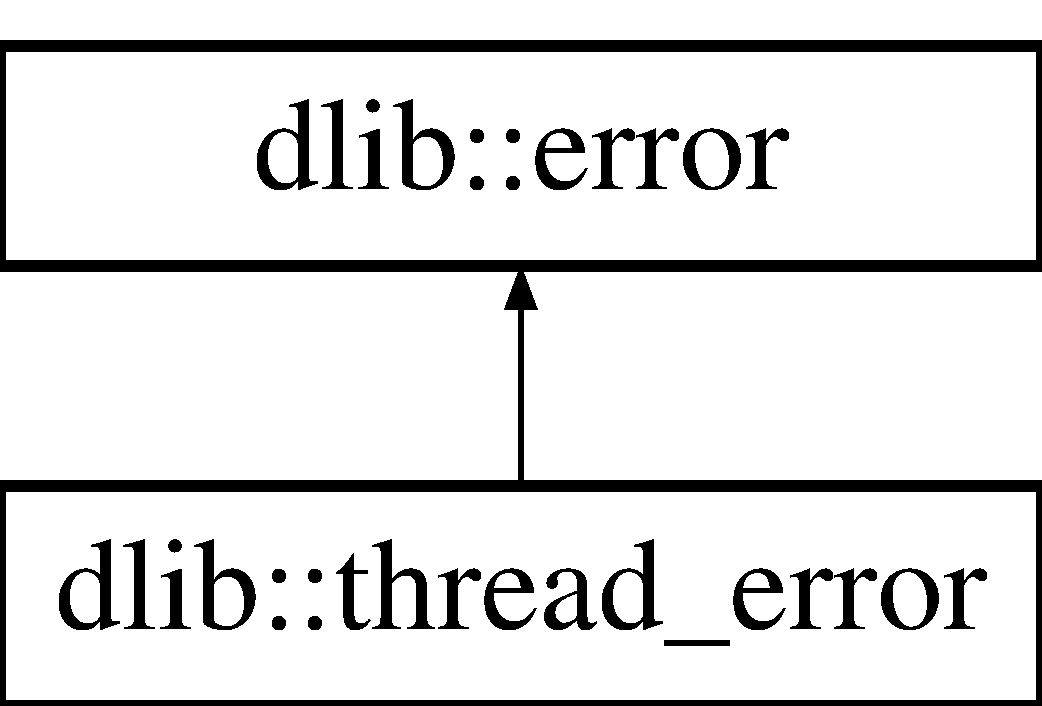
\includegraphics[height=2cm]{classdlib_1_1thread__error}
\end{center}
\end{figure}
\subsection*{Public Member Functions}
\begin{DoxyCompactItemize}
\item 
\hypertarget{classdlib_1_1thread__error_a414b496b877e3f3152fd306bffd87dc1}{
{\bfseries thread\_\-error} (error\_\-type t, const std::string \&a)}
\label{classdlib_1_1thread__error_a414b496b877e3f3152fd306bffd87dc1}

\item 
\hyperlink{classdlib_1_1thread__error_ae1bb1dd5554c6a336583d70935d3d11b}{thread\_\-error} (error\_\-type t)
\item 
\hyperlink{classdlib_1_1thread__error_a8221371c972598642867232a88eeefbe}{thread\_\-error} (const std::string \&a)
\item 
\hyperlink{classdlib_1_1thread__error_a9a609b7d05a464663ebdd787b2a6e6d1}{thread\_\-error} ()
\end{DoxyCompactItemize}


\subsection{Constructor \& Destructor Documentation}
\hypertarget{classdlib_1_1thread__error_ae1bb1dd5554c6a336583d70935d3d11b}{
\index{dlib::thread\_\-error@{dlib::thread\_\-error}!thread\_\-error@{thread\_\-error}}
\index{thread\_\-error@{thread\_\-error}!dlib::thread_error@{dlib::thread\_\-error}}
\subsubsection[{thread\_\-error}]{\setlength{\rightskip}{0pt plus 5cm}dlib::thread\_\-error::thread\_\-error (error\_\-type {\em t})\hspace{0.3cm}{\ttfamily  \mbox{[}inline\mbox{]}}}}
\label{classdlib_1_1thread__error_ae1bb1dd5554c6a336583d70935d3d11b}
ensures
\begin{DoxyItemize}
\item type == t
\item info == a ! 
\end{DoxyItemize}\hypertarget{classdlib_1_1thread__error_a8221371c972598642867232a88eeefbe}{
\index{dlib::thread\_\-error@{dlib::thread\_\-error}!thread\_\-error@{thread\_\-error}}
\index{thread\_\-error@{thread\_\-error}!dlib::thread_error@{dlib::thread\_\-error}}
\subsubsection[{thread\_\-error}]{\setlength{\rightskip}{0pt plus 5cm}dlib::thread\_\-error::thread\_\-error (const std::string \& {\em a})\hspace{0.3cm}{\ttfamily  \mbox{[}inline\mbox{]}}}}
\label{classdlib_1_1thread__error_a8221371c972598642867232a88eeefbe}
ensures
\begin{DoxyItemize}
\item type == t
\item info == \char`\"{}\char`\"{} ! 
\end{DoxyItemize}\hypertarget{classdlib_1_1thread__error_a9a609b7d05a464663ebdd787b2a6e6d1}{
\index{dlib::thread\_\-error@{dlib::thread\_\-error}!thread\_\-error@{thread\_\-error}}
\index{thread\_\-error@{thread\_\-error}!dlib::thread_error@{dlib::thread\_\-error}}
\subsubsection[{thread\_\-error}]{\setlength{\rightskip}{0pt plus 5cm}dlib::thread\_\-error::thread\_\-error ()\hspace{0.3cm}{\ttfamily  \mbox{[}inline\mbox{]}}}}
\label{classdlib_1_1thread__error_a9a609b7d05a464663ebdd787b2a6e6d1}
ensures
\begin{DoxyItemize}
\item type == ETHREAD
\item info == a ! 
\end{DoxyItemize}

The documentation for this class was generated from the following file:\begin{DoxyCompactItemize}
\item 
source/dlib/error.h\end{DoxyCompactItemize}

\hypertarget{classdlib_1_1timeout}{
\section{dlib::timeout Class Reference}
\label{classdlib_1_1timeout}\index{dlib::timeout@{dlib::timeout}}
}
\subsection*{Public Types}
\begin{DoxyCompactItemize}
\item 
\hypertarget{classdlib_1_1timeout_a8d5bec12c05ab4abbe113cbcfcb152b1}{
typedef timeout\_\-kernel\_\-1 {\bfseries kernel\_\-1a}}
\label{classdlib_1_1timeout_a8d5bec12c05ab4abbe113cbcfcb152b1}

\end{DoxyCompactItemize}


The documentation for this class was generated from the following file:\begin{DoxyCompactItemize}
\item 
source/dlib/timeout.h\end{DoxyCompactItemize}

\hypertarget{classdlib_1_1timer}{
\section{dlib::timer$<$ T $>$ Class Template Reference}
\label{classdlib_1_1timer}\index{dlib::timer@{dlib::timer}}
}
\subsection*{Public Types}
\begin{DoxyCompactItemize}
\item 
\hypertarget{classdlib_1_1timer_a024a6e6d2cd2bc6f91891f18101d34be}{
typedef timer\_\-kernel\_\-1$<$ T $>$ {\bfseries kernel\_\-1a}}
\label{classdlib_1_1timer_a024a6e6d2cd2bc6f91891f18101d34be}

\item 
\hypertarget{classdlib_1_1timer_ab269a67a2f5acb2548839f2a55d935db}{
typedef timer\_\-kernel\_\-2$<$ T $>$ {\bfseries kernel\_\-2a}}
\label{classdlib_1_1timer_ab269a67a2f5acb2548839f2a55d935db}

\end{DoxyCompactItemize}
\subsubsection*{template$<$typename T$>$ class dlib::timer$<$ T $>$}



The documentation for this class was generated from the following file:\begin{DoxyCompactItemize}
\item 
source/dlib/timer.h\end{DoxyCompactItemize}

\hypertarget{structdlib_1_1tmin}{
\section{dlib::tmin$<$ x, y, enabled $>$ Struct Template Reference}
\label{structdlib_1_1tmin}\index{dlib::tmin@{dlib::tmin}}
}


{\ttfamily \#include $<$algs.h$>$}\subsection*{Static Public Attributes}
\begin{DoxyCompactItemize}
\item 
\hypertarget{structdlib_1_1tmin_aa27a360ada93cb896c0beab29281eb5e}{
static const long {\bfseries value} = x}
\label{structdlib_1_1tmin_aa27a360ada93cb896c0beab29281eb5e}

\end{DoxyCompactItemize}


\subsection{Detailed Description}
\subsubsection*{template$<$long x, long y, typename enabled = void$>$ struct dlib::tmin$<$ x, y, enabled $>$}

A \hyperlink{structdlib_1_1tmin}{tmin}

This is a template to compute the min of two values at compile time

For example, abs$<$4,7$>$::value == 4 ! 

The documentation for this struct was generated from the following file:\begin{DoxyCompactItemize}
\item 
source/dlib/algs.h\end{DoxyCompactItemize}

\hypertarget{classdlib_1_1tokenizer}{
\section{dlib::tokenizer Class Reference}
\label{classdlib_1_1tokenizer}\index{dlib::tokenizer@{dlib::tokenizer}}
}
\subsection*{Public Types}
\begin{DoxyCompactItemize}
\item 
\hypertarget{classdlib_1_1tokenizer_a1c3ad3f7f55462ea12b2b35fdd8e2b8e}{
typedef tokenizer\_\-kernel\_\-1 {\bfseries kernel\_\-1a}}
\label{classdlib_1_1tokenizer_a1c3ad3f7f55462ea12b2b35fdd8e2b8e}

\item 
\hypertarget{classdlib_1_1tokenizer_a3c78f32311ba8cf41f75c3074124a2da}{
typedef tokenizer\_\-kernel\_\-c$<$ kernel\_\-1a $>$ {\bfseries kernel\_\-1a\_\-c}}
\label{classdlib_1_1tokenizer_a3c78f32311ba8cf41f75c3074124a2da}

\end{DoxyCompactItemize}


The documentation for this class was generated from the following file:\begin{DoxyCompactItemize}
\item 
source/dlib/tokenizer.h\end{DoxyCompactItemize}

\hypertarget{structdlib_1_1unsigned__type_3_01T_00_011_01_4}{
\section{dlib::unsigned\_\-type$<$ T, 1 $>$ Struct Template Reference}
\label{structdlib_1_1unsigned__type_3_01T_00_011_01_4}\index{dlib::unsigned\_\-type$<$ T, 1 $>$@{dlib::unsigned\_\-type$<$ T, 1 $>$}}
}
\subsection*{Public Types}
\begin{DoxyCompactItemize}
\item 
\hypertarget{structdlib_1_1unsigned__type_3_01T_00_011_01_4_a760176c4435cb28b5479093c468d7f4d}{
typedef uint8 {\bfseries type}}
\label{structdlib_1_1unsigned__type_3_01T_00_011_01_4_a760176c4435cb28b5479093c468d7f4d}

\end{DoxyCompactItemize}
\subsubsection*{template$<$typename T$>$ struct dlib::unsigned\_\-type$<$ T, 1 $>$}



The documentation for this struct was generated from the following file:\begin{DoxyCompactItemize}
\item 
source/dlib/uintn.h\end{DoxyCompactItemize}

\hypertarget{structdlib_1_1unsigned__type_3_01T_00_012_01_4}{
\section{dlib::unsigned\_\-type$<$ T, 2 $>$ Struct Template Reference}
\label{structdlib_1_1unsigned__type_3_01T_00_012_01_4}\index{dlib::unsigned\_\-type$<$ T, 2 $>$@{dlib::unsigned\_\-type$<$ T, 2 $>$}}
}
\subsection*{Public Types}
\begin{DoxyCompactItemize}
\item 
\hypertarget{structdlib_1_1unsigned__type_3_01T_00_012_01_4_a0a1193eee5098662c1b0822cf9891710}{
typedef uint16 {\bfseries type}}
\label{structdlib_1_1unsigned__type_3_01T_00_012_01_4_a0a1193eee5098662c1b0822cf9891710}

\end{DoxyCompactItemize}
\subsubsection*{template$<$typename T$>$ struct dlib::unsigned\_\-type$<$ T, 2 $>$}



The documentation for this struct was generated from the following file:\begin{DoxyCompactItemize}
\item 
source/dlib/uintn.h\end{DoxyCompactItemize}

\hypertarget{structdlib_1_1unsigned__type_3_01T_00_014_01_4}{
\section{dlib::unsigned\_\-type$<$ T, 4 $>$ Struct Template Reference}
\label{structdlib_1_1unsigned__type_3_01T_00_014_01_4}\index{dlib::unsigned\_\-type$<$ T, 4 $>$@{dlib::unsigned\_\-type$<$ T, 4 $>$}}
}
\subsection*{Public Types}
\begin{DoxyCompactItemize}
\item 
\hypertarget{structdlib_1_1unsigned__type_3_01T_00_014_01_4_aa5489ca71a60073699dc35e70cb7f495}{
typedef uint32 {\bfseries type}}
\label{structdlib_1_1unsigned__type_3_01T_00_014_01_4_aa5489ca71a60073699dc35e70cb7f495}

\end{DoxyCompactItemize}
\subsubsection*{template$<$typename T$>$ struct dlib::unsigned\_\-type$<$ T, 4 $>$}



The documentation for this struct was generated from the following file:\begin{DoxyCompactItemize}
\item 
source/dlib/uintn.h\end{DoxyCompactItemize}

\hypertarget{structdlib_1_1unsigned__type_3_01T_00_018_01_4}{
\section{dlib::unsigned\_\-type$<$ T, 8 $>$ Struct Template Reference}
\label{structdlib_1_1unsigned__type_3_01T_00_018_01_4}\index{dlib::unsigned\_\-type$<$ T, 8 $>$@{dlib::unsigned\_\-type$<$ T, 8 $>$}}
}
\subsection*{Public Types}
\begin{DoxyCompactItemize}
\item 
\hypertarget{structdlib_1_1unsigned__type_3_01T_00_018_01_4_ab82a5b3135e4a9f41a8ddf7cd5a5df07}{
typedef \hyperlink{namespacedlib_a61113f8b6b3e4ccb66deca9355c8f65d}{uint64} {\bfseries type}}
\label{structdlib_1_1unsigned__type_3_01T_00_018_01_4_ab82a5b3135e4a9f41a8ddf7cd5a5df07}

\end{DoxyCompactItemize}
\subsubsection*{template$<$typename T$>$ struct dlib::unsigned\_\-type$<$ T, 8 $>$}



The documentation for this struct was generated from the following file:\begin{DoxyCompactItemize}
\item 
source/dlib/uintn.h\end{DoxyCompactItemize}

\hypertarget{classWorld}{
\section{World Class Reference}
\label{classWorld}\index{World@{World}}
}
\subsection*{Public Member Functions}
\begin{DoxyCompactItemize}
\item 
\hyperlink{classWorld_a6ce0c6ba5ce813c0ec0b910a88e09d64}{World} (CL\_\-DisplayWindow \&)
\item 
virtual \hyperlink{classWorld_a8c73fba541a5817fff65147ba47cd827}{$\sim$World} ()
\item 
int \hyperlink{classWorld_a0e3eea96c33cd34c6a3b05bba6b88ef5}{run} ()
\item 
void \hyperlink{classWorld_a6703e4f889e72198e0ede0cd23864792}{addOverlay} (\hyperlink{classOverlay}{Overlay} $\ast$)
\item 
void \hyperlink{classWorld_ad74a2b078f0173249b04e3da2982d081}{addGameObject} (\hyperlink{classGameObject}{GameObject} $\ast$)
\item 
\hypertarget{classWorld_a147bbd276bcff24c6d5c6ade85145545}{
CL\_\-GraphicContext $\ast$ {\bfseries getGC} (void)}
\label{classWorld_a147bbd276bcff24c6d5c6ade85145545}

\item 
\hypertarget{classWorld_ae62ed957ab6a1c8ffd58b5eeda690ce9}{
CL\_\-ResourceManager $\ast$ {\bfseries getRM} (void)}
\label{classWorld_ae62ed957ab6a1c8ffd58b5eeda690ce9}

\end{DoxyCompactItemize}


\subsection{Constructor \& Destructor Documentation}
\hypertarget{classWorld_a6ce0c6ba5ce813c0ec0b910a88e09d64}{
\index{World@{World}!World@{World}}
\index{World@{World}!World@{World}}
\subsubsection[{World}]{\setlength{\rightskip}{0pt plus 5cm}World::World (CL\_\-DisplayWindow \& {\em display\_\-window})}}
\label{classWorld_a6ce0c6ba5ce813c0ec0b910a88e09d64}
Creates the game world and sets up initial contents. \hypertarget{classWorld_a8c73fba541a5817fff65147ba47cd827}{
\index{World@{World}!$\sim$World@{$\sim$World}}
\index{$\sim$World@{$\sim$World}!World@{World}}
\subsubsection[{$\sim$World}]{\setlength{\rightskip}{0pt plus 5cm}World::$\sim$World ()\hspace{0.3cm}{\ttfamily  \mbox{[}virtual\mbox{]}}}}
\label{classWorld_a8c73fba541a5817fff65147ba47cd827}
Destructor. 

\subsection{Member Function Documentation}
\hypertarget{classWorld_ad74a2b078f0173249b04e3da2982d081}{
\index{World@{World}!addGameObject@{addGameObject}}
\index{addGameObject@{addGameObject}!World@{World}}
\subsubsection[{addGameObject}]{\setlength{\rightskip}{0pt plus 5cm}void World::addGameObject ({\bf GameObject} $\ast$ {\em game\_\-object})}}
\label{classWorld_ad74a2b078f0173249b04e3da2982d081}
Adds a game object to the world. \hypertarget{classWorld_a6703e4f889e72198e0ede0cd23864792}{
\index{World@{World}!addOverlay@{addOverlay}}
\index{addOverlay@{addOverlay}!World@{World}}
\subsubsection[{addOverlay}]{\setlength{\rightskip}{0pt plus 5cm}void World::addOverlay ({\bf Overlay} $\ast$ {\em overlay})}}
\label{classWorld_a6703e4f889e72198e0ede0cd23864792}
Adds an overlay object to the world. \hypertarget{classWorld_a0e3eea96c33cd34c6a3b05bba6b88ef5}{
\index{World@{World}!run@{run}}
\index{run@{run}!World@{World}}
\subsubsection[{run}]{\setlength{\rightskip}{0pt plus 5cm}int World::run ()}}
\label{classWorld_a0e3eea96c33cd34c6a3b05bba6b88ef5}
Initiates the game loop. 

The documentation for this class was generated from the following files:\begin{DoxyCompactItemize}
\item 
World.h\item 
World.cpp\end{DoxyCompactItemize}

\hypertarget{classdlib_1_1xml__parser}{
\section{dlib::xml\_\-parser Class Reference}
\label{classdlib_1_1xml__parser}\index{dlib::xml\_\-parser@{dlib::xml\_\-parser}}
}
\subsection*{Public Types}
\begin{DoxyCompactItemize}
\item 
\hypertarget{classdlib_1_1xml__parser_a5961701f09130b8b44f399cb9ce4e71b}{
typedef xml\_\-parser\_\-kernel\_\-1$<$ map1a, stack1a, seq\_\-dh2a, seq\_\-eh2a $>$ {\bfseries kernel\_\-1a}}
\label{classdlib_1_1xml__parser_a5961701f09130b8b44f399cb9ce4e71b}

\item 
\hypertarget{classdlib_1_1xml__parser_a67fe02d8b691747b1710405b60058563}{
typedef xml\_\-parser\_\-kernel\_\-c$<$ kernel\_\-1a\_\-c\_\-impl $>$ {\bfseries kernel\_\-1a\_\-c}}
\label{classdlib_1_1xml__parser_a67fe02d8b691747b1710405b60058563}

\end{DoxyCompactItemize}


The documentation for this class was generated from the following file:\begin{DoxyCompactItemize}
\item 
source/dlib/xml\_\-parser.h\end{DoxyCompactItemize}

\hypertarget{structdlib_1_1is__convertible_1_1yes__type}{
\section{dlib::is\_\-convertible$<$ from, to $>$::yes\_\-type Struct Reference}
\label{structdlib_1_1is__convertible_1_1yes__type}\index{dlib::is\_\-convertible::yes\_\-type@{dlib::is\_\-convertible::yes\_\-type}}
}
\subsection*{Public Attributes}
\begin{DoxyCompactItemize}
\item 
\hypertarget{structdlib_1_1is__convertible_1_1yes__type_ab16a8cf639bd536ca54e3a750ca028e7}{
char {\bfseries a}}
\label{structdlib_1_1is__convertible_1_1yes__type_ab16a8cf639bd536ca54e3a750ca028e7}

\end{DoxyCompactItemize}
\subsubsection*{template$<$typename from, typename to$>$ struct dlib::is\_\-convertible$<$ from, to $>$::yes\_\-type}



The documentation for this struct was generated from the following file:\begin{DoxyCompactItemize}
\item 
source/dlib/algs.h\end{DoxyCompactItemize}

\chapter{File Documentation}
\hypertarget{ApplicationModule_8cpp}{
\section{source/ApplicationModule.cpp File Reference}
\label{ApplicationModule_8cpp}\index{source/ApplicationModule.cpp@{source/ApplicationModule.cpp}}
}
{\ttfamily \#include \char`\"{}ApplicationModule.h\char`\"{}}\par
{\ttfamily \#include \char`\"{}misc/logging.h\char`\"{}}\par


\subsection{Detailed Description}
Created on: 15 Feb 2010

\begin{DoxyAuthor}{Author}
Gregory Doran $<$www.gregorydoran.co.uk$>$ 
\end{DoxyAuthor}

\hypertarget{ApplicationModule_8h}{
\section{source/ApplicationModule.h File Reference}
\label{ApplicationModule_8h}\index{source/ApplicationModule.h@{source/ApplicationModule.h}}
}
{\ttfamily \#include \char`\"{}ApplicationModuleExitCode.h\char`\"{}}\par
{\ttfamily \#include $<$ClanLib/core.h$>$}\par
{\ttfamily \#include $<$ClanLib/gui.h$>$}\par
\subsection*{Classes}
\begin{DoxyCompactItemize}
\item 
class \hyperlink{classApplicationModule}{ApplicationModule}
\end{DoxyCompactItemize}


\subsection{Detailed Description}
Created on: 15 Feb 2010

\begin{DoxyAuthor}{Author}
Gregory Doran $<$www.gregorydoran.co.uk$>$ 
\end{DoxyAuthor}

\hypertarget{ApplicationModuleExitCode_8h}{
\section{source/ApplicationModuleExitCode.h File Reference}
\label{ApplicationModuleExitCode_8h}\index{source/ApplicationModuleExitCode.h@{source/ApplicationModuleExitCode.h}}
}
\subsection*{Enumerations}
\begin{DoxyCompactItemize}
\item 
enum {\bfseries ApplicationModuleExitCode} \{ \par
{\bfseries no\_\-exit} =  0, 
{\bfseries exit\_\-application} =  1, 
{\bfseries exit\_\-module\_\-and\_\-load\_\-game} =  2, 
{\bfseries exit\_\-module\_\-and\_\-load\_\-editor} =  3, 
\par
{\bfseries exit\_\-module\_\-and\_\-load\_\-main\_\-menu} =  4
 \}
\end{DoxyCompactItemize}


\subsection{Detailed Description}
Created on: 15 Feb 2010 \begin{DoxyAuthor}{Author}
Gregory Doran $<$www.gregorydoran.co.uk$>$ 
\end{DoxyAuthor}

\hypertarget{Editor_8cpp}{
\section{source/editor/Editor.cpp File Reference}
\label{Editor_8cpp}\index{source/editor/Editor.cpp@{source/editor/Editor.cpp}}
}
{\ttfamily \#include \char`\"{}Editor.h\char`\"{}}\par
{\ttfamily \#include \char`\"{}../misc/logging.h\char`\"{}}\par


\subsection{Detailed Description}
Created on: 15 Feb 2010 \begin{DoxyAuthor}{Author}
Gregory Doran $<$www.gregorydoran.co.uk$>$ 
\end{DoxyAuthor}

\hypertarget{Editor_8h}{
\section{source/editor/Editor.h File Reference}
\label{Editor_8h}\index{source/editor/Editor.h@{source/editor/Editor.h}}
}
{\ttfamily \#include $<$ClanLib/display.h$>$}\par
{\ttfamily \#include $<$ClanLib/core.h$>$}\par
{\ttfamily \#include \char`\"{}../ApplicationModule.h\char`\"{}}\par
\subsection*{Classes}
\begin{DoxyCompactItemize}
\item 
class \hyperlink{classEditor}{Editor}
\end{DoxyCompactItemize}


\subsection{Detailed Description}
Created on: 15 Feb 2010 \begin{DoxyAuthor}{Author}
Gregory Doran $<$www.gregorydoran.co.uk$>$ 
\end{DoxyAuthor}

\hypertarget{FloorTest_8cpp}{
\section{source/game/FloorTest.cpp File Reference}
\label{FloorTest_8cpp}\index{source/game/FloorTest.cpp@{source/game/FloorTest.cpp}}
}


\subsection{Detailed Description}
Created on: 18 Jan 2010 \begin{DoxyAuthor}{Author}
Gregory Doran $<$www.gregorydoran.co.uk$>$ 
\end{DoxyAuthor}

\hypertarget{FloorTest_8h}{
\section{source/game/FloorTest.h File Reference}
\label{FloorTest_8h}\index{source/game/FloorTest.h@{source/game/FloorTest.h}}
}
{\ttfamily \#include \char`\"{}Overlay.h\char`\"{}}\par


\subsection{Detailed Description}
Created on: 18 Jan 2010 \begin{DoxyAuthor}{Author}
Gregory Doran $<$www.gregorydoran.co.uk$>$ 
\end{DoxyAuthor}

\hypertarget{GameObject_8cpp}{
\section{source/game/GameObject.cpp File Reference}
\label{GameObject_8cpp}\index{source/game/GameObject.cpp@{source/game/GameObject.cpp}}
}
{\ttfamily \#include \char`\"{}GameObject.h\char`\"{}}\par
{\ttfamily \#include $<$ClanLib/core.h$>$}\par
{\ttfamily \#include \char`\"{}../misc/logging.h\char`\"{}}\par
{\ttfamily \#include \char`\"{}Scene.h\char`\"{}}\par
{\ttfamily \#include \char`\"{}World.h\char`\"{}}\par


\subsection{Detailed Description}
Created on: 25 Dec 2009 \begin{DoxyAuthor}{Author}
Gregory Doran $<$www.gregorydoran.co.uk$>$ 
\end{DoxyAuthor}

\hypertarget{GameObject_8h}{
\section{source/game/GameObject.h File Reference}
\label{GameObject_8h}\index{source/game/GameObject.h@{source/game/GameObject.h}}
}
{\ttfamily \#include $<$ClanLib/core.h$>$}\par
{\ttfamily \#include $<$ClanLib/display.h$>$}\par
\subsection*{Classes}
\begin{DoxyCompactItemize}
\item 
class \hyperlink{classGameObject}{GameObject}
\end{DoxyCompactItemize}
\subsection*{Defines}
\begin{DoxyCompactItemize}
\item 
\hypertarget{GameObject_8h_aac324b2e1c958bb9b0c0c342a35f20f1}{
\#define {\bfseries SPRITE\_\-N}~0}
\label{GameObject_8h_aac324b2e1c958bb9b0c0c342a35f20f1}

\item 
\hypertarget{GameObject_8h_ac937fbcbfed8f2a1ce5219f7011317c7}{
\#define {\bfseries SPRITE\_\-NE}~1}
\label{GameObject_8h_ac937fbcbfed8f2a1ce5219f7011317c7}

\item 
\hypertarget{GameObject_8h_a5148e80336d53387cde98653d9d724a9}{
\#define {\bfseries SPRITE\_\-E}~2}
\label{GameObject_8h_a5148e80336d53387cde98653d9d724a9}

\item 
\hypertarget{GameObject_8h_a8dff60420186fcd1a69c28e1803bce89}{
\#define {\bfseries SPRITE\_\-SE}~3}
\label{GameObject_8h_a8dff60420186fcd1a69c28e1803bce89}

\item 
\hypertarget{GameObject_8h_a34b36bf9dc0b7e543ef39d00f88b7e18}{
\#define {\bfseries SPRITE\_\-S}~4}
\label{GameObject_8h_a34b36bf9dc0b7e543ef39d00f88b7e18}

\item 
\hypertarget{GameObject_8h_a82494b8b421d8d6e2dc97c796271e50d}{
\#define {\bfseries SPRITE\_\-SW}~5}
\label{GameObject_8h_a82494b8b421d8d6e2dc97c796271e50d}

\item 
\hypertarget{GameObject_8h_a0d6645b87c7176daacde7f87a4c6d0e7}{
\#define {\bfseries SPRITE\_\-W}~6}
\label{GameObject_8h_a0d6645b87c7176daacde7f87a4c6d0e7}

\item 
\hypertarget{GameObject_8h_a920b8b81e0b42f54614d01c24589c0d1}{
\#define {\bfseries SPRITE\_\-NW}~7}
\label{GameObject_8h_a920b8b81e0b42f54614d01c24589c0d1}

\end{DoxyCompactItemize}


\subsection{Detailed Description}
Created on: 25 Dec 2009 \begin{DoxyAuthor}{Author}
Gregory Doran $<$www.gregorydoran.co.uk$>$ 
\end{DoxyAuthor}

\hypertarget{IsometricConversions_8cpp}{
\section{source/game/IsometricConversions.cpp File Reference}
\label{IsometricConversions_8cpp}\index{source/game/IsometricConversions.cpp@{source/game/IsometricConversions.cpp}}
}
{\ttfamily \#include \char`\"{}IsometricConversions.h\char`\"{}}\par


\subsection{Detailed Description}
Created on: 12 Dec 2009 \begin{DoxyAuthor}{Author}
Gregory Doran $<$www.gregorydoran.co.uk$>$ 
\end{DoxyAuthor}

\hypertarget{IsometricConversions_8h}{
\section{source/game/IsometricConversions.h File Reference}
\label{IsometricConversions_8h}\index{source/game/IsometricConversions.h@{source/game/IsometricConversions.h}}
}
{\ttfamily \#include $<$ClanLib/core.h$>$}\par
\subsection*{Classes}
\begin{DoxyCompactItemize}
\item 
class \hyperlink{classIsometricConversions}{IsometricConversions}
\end{DoxyCompactItemize}


\subsection{Detailed Description}
Created on: 12 Dec 2009 \begin{DoxyAuthor}{Author}
Gregory Doran $<$www.gregorydoran.co.uk$>$ 
\end{DoxyAuthor}

\hypertarget{IsometricGrid_8cpp}{
\section{source/game/IsometricGrid.cpp File Reference}
\label{IsometricGrid_8cpp}\index{source/game/IsometricGrid.cpp@{source/game/IsometricGrid.cpp}}
}
{\ttfamily \#include \char`\"{}IsometricGrid.h\char`\"{}}\par
{\ttfamily \#include \char`\"{}IsometricConversions.h\char`\"{}}\par
{\ttfamily \#include \char`\"{}World.h\char`\"{}}\par
{\ttfamily \#include $<$ClanLib/core.h$>$}\par


\subsection{Detailed Description}
Created on: 12 Dec 2009 \begin{DoxyAuthor}{Author}
Gregory Doran $<$www.gregorydoran.co.uk$>$ 
\end{DoxyAuthor}

\hypertarget{IsometricGrid_8h}{
\section{source/game/IsometricGrid.h File Reference}
\label{IsometricGrid_8h}\index{source/game/IsometricGrid.h@{source/game/IsometricGrid.h}}
}
{\ttfamily \#include \char`\"{}Overlay.h\char`\"{}}\par
{\ttfamily \#include $<$ClanLib/display.h$>$}\par
\subsection*{Classes}
\begin{DoxyCompactItemize}
\item 
class \hyperlink{classIsometricGrid}{IsometricGrid}
\end{DoxyCompactItemize}


\subsection{Detailed Description}
Created on: 12 Dec 2009 \begin{DoxyAuthor}{Author}
Gregory Doran $<$www.gregorydoran.co.uk$>$ 
\end{DoxyAuthor}

\hypertarget{MoveableGameObject_8cpp}{
\section{source/game/MoveableGameObject.cpp File Reference}
\label{MoveableGameObject_8cpp}\index{source/game/MoveableGameObject.cpp@{source/game/MoveableGameObject.cpp}}
}
{\ttfamily \#include \char`\"{}MoveableGameObject.h\char`\"{}}\par
{\ttfamily \#include \char`\"{}IsometricConversions.h\char`\"{}}\par
{\ttfamily \#include \char`\"{}World.h\char`\"{}}\par
{\ttfamily \#include $<$ClanLib/core.h$>$}\par


\subsection{Detailed Description}
Created on: 25 Dec 2009 \begin{DoxyAuthor}{Author}
Gregory Doran $<$www.gregorydoran.co.uk$>$ 
\end{DoxyAuthor}

\hypertarget{MoveableGameObject_8h}{
\section{source/game/MoveableGameObject.h File Reference}
\label{MoveableGameObject_8h}\index{source/game/MoveableGameObject.h@{source/game/MoveableGameObject.h}}
}
{\ttfamily \#include \char`\"{}GameObject.h\char`\"{}}\par
\subsection*{Classes}
\begin{DoxyCompactItemize}
\item 
class \hyperlink{classMoveableGameObject}{MoveableGameObject}
\end{DoxyCompactItemize}


\subsection{Detailed Description}
Created on: 25 Dec 2009 \begin{DoxyAuthor}{Author}
Gregory Doran $<$www.gregorydoran.co.uk$>$ 
\end{DoxyAuthor}

\hypertarget{Overlay_8cpp}{
\section{source/game/Overlay.cpp File Reference}
\label{Overlay_8cpp}\index{source/game/Overlay.cpp@{source/game/Overlay.cpp}}
}
{\ttfamily \#include \char`\"{}Overlay.h\char`\"{}}\par


\subsection{Detailed Description}
Created on: 12 Dec 2009 \begin{DoxyAuthor}{Author}
Gregory Doran $<$www.gregorydoran.co.uk$>$ 
\end{DoxyAuthor}

\hypertarget{Overlay_8h}{
\section{source/game/Overlay.h File Reference}
\label{Overlay_8h}\index{source/game/Overlay.h@{source/game/Overlay.h}}
}
\subsection*{Classes}
\begin{DoxyCompactItemize}
\item 
class \hyperlink{classOverlay}{Overlay}
\end{DoxyCompactItemize}


\subsection{Detailed Description}
Created on: 12 Dec 2009 \begin{DoxyAuthor}{Author}
Gregory Doran $<$www.gregorydoran.co.uk$>$ 
\end{DoxyAuthor}

\hypertarget{PlayerCharacter_8cpp}{
\section{source/game/PlayerCharacter.cpp File Reference}
\label{PlayerCharacter_8cpp}\index{source/game/PlayerCharacter.cpp@{source/game/PlayerCharacter.cpp}}
}
{\ttfamily \#include \char`\"{}PlayerCharacter.h\char`\"{}}\par
{\ttfamily \#include $<$ClanLib/core.h$>$}\par
{\ttfamily \#include \char`\"{}World.h\char`\"{}}\par


\subsection{Detailed Description}
Created on: 26 Dec 2009 \begin{DoxyAuthor}{Author}
Gregory Doran $<$www.gregorydoran.co.uk$>$ 
\end{DoxyAuthor}

\hypertarget{PlayerCharacter_8h}{
\section{source/game/game\_\-objects/PlayerCharacter.h File Reference}
\label{PlayerCharacter_8h}\index{source/game/game\_\-objects/PlayerCharacter.h@{source/game/game\_\-objects/PlayerCharacter.h}}
}
{\ttfamily \#include \char`\"{}../GameObject.h\char`\"{}}\par
\subsection*{Classes}
\begin{DoxyCompactItemize}
\item 
class \hyperlink{classPlayerCharacter}{PlayerCharacter}
\end{DoxyCompactItemize}


\subsection{Detailed Description}
Created on: 26 Dec 2009 \begin{DoxyAuthor}{Author}
Gregory Doran $<$www.gregorydoran.co.uk$>$ 
\end{DoxyAuthor}

\hypertarget{RandomGenerator_8cpp}{
\section{source/game/RandomGenerator.cpp File Reference}
\label{RandomGenerator_8cpp}\index{source/game/RandomGenerator.cpp@{source/game/RandomGenerator.cpp}}
}
{\ttfamily \#include \char`\"{}RandomGenerator.h\char`\"{}}\par
{\ttfamily \#include $<$cstdlib$>$}\par


\subsection{Detailed Description}
Created on: 2 Dec 2009 \begin{DoxyAuthor}{Author}
Gregory Doran $<$www.gregorydoran.co.uk$>$ 
\end{DoxyAuthor}

\hypertarget{RandomGenerator_8h}{
\section{source/game/RandomGenerator.h File Reference}
\label{RandomGenerator_8h}\index{source/game/RandomGenerator.h@{source/game/RandomGenerator.h}}
}
\subsection*{Classes}
\begin{DoxyCompactItemize}
\item 
class \hyperlink{classRandomGenerator}{RandomGenerator}
\end{DoxyCompactItemize}


\subsection{Detailed Description}
Created on: 2 Dec 2009 \begin{DoxyAuthor}{Author}
Gregory Doran $<$www.gregorydoran.co.uk$>$ 
\end{DoxyAuthor}

\hypertarget{World_8cpp}{
\section{source/game/World.cpp File Reference}
\label{World_8cpp}\index{source/game/World.cpp@{source/game/World.cpp}}
}
{\ttfamily \#include \char`\"{}World.h\char`\"{}}\par
{\ttfamily \#include \char`\"{}IsometricGrid.h\char`\"{}}\par
{\ttfamily \#include \char`\"{}PlayerCharacter.h\char`\"{}}\par
{\ttfamily \#include \char`\"{}GameObject.h\char`\"{}}\par
{\ttfamily \#include \char`\"{}Overlay.h\char`\"{}}\par
{\ttfamily \#include \char`\"{}../Application.h\char`\"{}}\par
{\ttfamily \#include \char`\"{}../misc/logging.h\char`\"{}}\par
{\ttfamily \#include \char`\"{}../mystery\_\-xml/Plot.h\char`\"{}}\par


\subsection{Detailed Description}
Created on: 6 Dec 2009 \begin{DoxyAuthor}{Author}
Gregory Doran $<$www.gregorydoran.co.uk$>$ 
\end{DoxyAuthor}

\hypertarget{World_8h}{
\section{source/game/World.h File Reference}
\label{World_8h}\index{source/game/World.h@{source/game/World.h}}
}
{\ttfamily \#include $<$ClanLib/display.h$>$}\par
{\ttfamily \#include $<$ClanLib/core.h$>$}\par
{\ttfamily \#include $<$ClanLib/sound.h$>$}\par
{\ttfamily \#include $<$ClanLib/mikmod.h$>$}\par
{\ttfamily \#include $<$ClanLib/vorbis.h$>$}\par
{\ttfamily \#include $<$list$>$}\par
{\ttfamily \#include \char`\"{}../ApplicationModule.h\char`\"{}}\par
\subsection*{Classes}
\begin{DoxyCompactItemize}
\item 
class \hyperlink{classWorld}{World}
\end{DoxyCompactItemize}


\subsection{Detailed Description}
Created on: 6 Dec 2009 \begin{DoxyAuthor}{Author}
Gregory Doran $<$www.gregorydoran.co.uk$>$ 
\end{DoxyAuthor}

\hypertarget{MainMenu_8cpp}{
\section{source/main\_\-menu/MainMenu.cpp File Reference}
\label{MainMenu_8cpp}\index{source/main\_\-menu/MainMenu.cpp@{source/main\_\-menu/MainMenu.cpp}}
}
{\ttfamily \#include \char`\"{}MainMenu.h\char`\"{}}\par
{\ttfamily \#include \char`\"{}../misc/logging.h\char`\"{}}\par


\subsection{Detailed Description}
Created on: 15 Feb 2010 \begin{DoxyAuthor}{Author}
Gregory Doran $<$www.gregorydoran.co.uk$>$ 
\end{DoxyAuthor}

\hypertarget{MainMenu_8h}{
\section{source/main\_\-menu/MainMenu.h File Reference}
\label{MainMenu_8h}\index{source/main\_\-menu/MainMenu.h@{source/main\_\-menu/MainMenu.h}}
}
{\ttfamily \#include $<$ClanLib/display.h$>$}\par
{\ttfamily \#include $<$ClanLib/core.h$>$}\par
{\ttfamily \#include $<$ClanLib/gui.h$>$}\par
{\ttfamily \#include \char`\"{}../ApplicationModule.h\char`\"{}}\par
\subsection*{Classes}
\begin{DoxyCompactItemize}
\item 
class \hyperlink{classMainMenu}{MainMenu}
\end{DoxyCompactItemize}


\subsection{Detailed Description}
Created on: 15 Feb 2010 \begin{DoxyAuthor}{Author}
Gregory Doran $<$www.gregorydoran.co.uk$>$ 
\end{DoxyAuthor}

\hypertarget{logging_8h}{
\section{source/misc/logging.h File Reference}
\label{logging_8h}\index{source/misc/logging.h@{source/misc/logging.h}}
}
\subsection*{Defines}
\begin{DoxyCompactItemize}
\item 
\hypertarget{logging_8h_a130224df8c6bf22a688e3cb74a45689a}{
\#define {\bfseries LOG\_\-LEVEL\_\-DEBUG}~5}
\label{logging_8h_a130224df8c6bf22a688e3cb74a45689a}

\item 
\hypertarget{logging_8h_a14f43a1fab62b98fc88603cdb988de3d}{
\#define {\bfseries LOG\_\-LEVEL\_\-WARN}~2}
\label{logging_8h_a14f43a1fab62b98fc88603cdb988de3d}

\item 
\hypertarget{logging_8h_a2e25fe130cf710da4ad800747fdd51f3}{
\#define {\bfseries LOG\_\-LEVEL\_\-INFO}~0}
\label{logging_8h_a2e25fe130cf710da4ad800747fdd51f3}

\item 
\hypertarget{logging_8h_ab6fecd8522a725f49d8d3678f13f5e8a}{
\#define {\bfseries DEBUG\_\-MSG}(message)}
\label{logging_8h_ab6fecd8522a725f49d8d3678f13f5e8a}

\end{DoxyCompactItemize}


\subsection{Detailed Description}
Contains pre-\/processor macros for logging. If LOG\_\-DEBUG\_\-MESSAGES is not defined then the code isn't compiled into the application.

Created on: 16 Jan 2010 \begin{DoxyAuthor}{Author}
Gregory Doran $<$www.gregorydoran.co.uk$>$ 
\end{DoxyAuthor}

\hypertarget{Decisions_8cpp}{
\section{source/mystery\_\-xml/Decisions.cpp File Reference}
\label{Decisions_8cpp}\index{source/mystery\_\-xml/Decisions.cpp@{source/mystery\_\-xml/Decisions.cpp}}
}
{\ttfamily \#include \char`\"{}Decisions.h\char`\"{}}\par
{\ttfamily \#include \char`\"{}Decision.h\char`\"{}}\par
{\ttfamily \#include \char`\"{}Plot.h\char`\"{}}\par
{\ttfamily \#include \char`\"{}../misc/logging.h\char`\"{}}\par


\subsection{Detailed Description}
Created on: 16 Jan 2010 \begin{DoxyAuthor}{Author}
Gregory Doran $<$www.gregorydoran.co.uk$>$ 
\end{DoxyAuthor}

\hypertarget{Decisions_8h}{
\section{source/mystery\_\-xml/Decisions.h File Reference}
\label{Decisions_8h}\index{source/mystery\_\-xml/Decisions.h@{source/mystery\_\-xml/Decisions.h}}
}
{\ttfamily \#include $<$ClanLib/core.h$>$}\par
{\ttfamily \#include $<$list$>$}\par
{\ttfamily \#include \char`\"{}Decision.h\char`\"{}}\par
\subsection*{Classes}
\begin{DoxyCompactItemize}
\item 
class \hyperlink{classDecisions}{Decisions}
\end{DoxyCompactItemize}


\subsection{Detailed Description}
Created on: 16 Jan 2010 \begin{DoxyAuthor}{Author}
Gregory Doran $<$www.gregorydoran.co.uk$>$ 
\end{DoxyAuthor}

\hypertarget{Option_8cpp}{
\section{source/mystery\_\-xml/Option.cpp File Reference}
\label{Option_8cpp}\index{source/mystery\_\-xml/Option.cpp@{source/mystery\_\-xml/Option.cpp}}
}
{\ttfamily \#include \char`\"{}Option.h\char`\"{}}\par
{\ttfamily \#include \char`\"{}Plot.h\char`\"{}}\par
{\ttfamily \#include \char`\"{}../misc/logging.h\char`\"{}}\par


\subsection{Detailed Description}
Created on: 16 Jan 2010 \begin{DoxyAuthor}{Author}
Gregory Doran $<$www.gregorydoran.co.uk$>$ 
\end{DoxyAuthor}

\hypertarget{Option_8h}{
\section{source/mystery\_\-xml/Option.h File Reference}
\label{Option_8h}\index{source/mystery\_\-xml/Option.h@{source/mystery\_\-xml/Option.h}}
}
{\ttfamily \#include $<$ClanLib/core.h$>$}\par
\subsection*{Classes}
\begin{DoxyCompactItemize}
\item 
class \hyperlink{classOption}{Option}
\end{DoxyCompactItemize}


\subsection{Detailed Description}
Created on: 16 Jan 2010 \begin{DoxyAuthor}{Author}
Gregory Doran $<$www.gregorydoran.co.uk$>$ 
\end{DoxyAuthor}

\hypertarget{Options_8cpp}{
\section{source/mystery\_\-xml/Options.cpp File Reference}
\label{Options_8cpp}\index{source/mystery\_\-xml/Options.cpp@{source/mystery\_\-xml/Options.cpp}}
}
{\ttfamily \#include \char`\"{}Options.h\char`\"{}}\par
{\ttfamily \#include \char`\"{}Plot.h\char`\"{}}\par
{\ttfamily \#include \char`\"{}Result.h\char`\"{}}\par
{\ttfamily \#include \char`\"{}../misc/logging.h\char`\"{}}\par


\subsection{Detailed Description}
Created on: 16 Jan 2010 \begin{DoxyAuthor}{Author}
Gregory Doran $<$www.gregorydoran.co.uk$>$ 
\end{DoxyAuthor}

\hypertarget{Options_8h}{
\section{source/mystery\_\-xml/Options.h File Reference}
\label{Options_8h}\index{source/mystery\_\-xml/Options.h@{source/mystery\_\-xml/Options.h}}
}
{\ttfamily \#include $<$ClanLib/core.h$>$}\par
{\ttfamily \#include $<$list$>$}\par
{\ttfamily \#include \char`\"{}Option.h\char`\"{}}\par
\subsection*{Classes}
\begin{DoxyCompactItemize}
\item 
class \hyperlink{classOptions}{Options}
\end{DoxyCompactItemize}


\subsection{Detailed Description}
Created on: 16 Jan 2010 \begin{DoxyAuthor}{Author}
Gregory Doran $<$www.gregorydoran.co.uk$>$ 
\end{DoxyAuthor}

\hypertarget{Plot_8cpp}{
\section{source/mystery\_\-xml/Plot.cpp File Reference}
\label{Plot_8cpp}\index{source/mystery\_\-xml/Plot.cpp@{source/mystery\_\-xml/Plot.cpp}}
}
{\ttfamily \#include \char`\"{}Plot.h\char`\"{}}\par
{\ttfamily \#include \char`\"{}../misc/logging.h\char`\"{}}\par
{\ttfamily \#include \char`\"{}Option.h\char`\"{}}\par


\subsection{Detailed Description}
Created on: 15 Jan 2010 \begin{DoxyAuthor}{Author}
Gregory Doran $<$www.gregorydoran.co.uk$>$ 
\end{DoxyAuthor}

\hypertarget{Plot_8h}{
\section{source/mystery\_\-xml/Plot.h File Reference}
\label{Plot_8h}\index{source/mystery\_\-xml/Plot.h@{source/mystery\_\-xml/Plot.h}}
}
{\ttfamily \#include $<$ClanLib/core.h$>$}\par
{\ttfamily \#include $<$map$>$}\par
{\ttfamily \#include \char`\"{}Decisions.h\char`\"{}}\par
\subsection*{Classes}
\begin{DoxyCompactItemize}
\item 
class \hyperlink{classPlot}{Plot}
\end{DoxyCompactItemize}
\subsection*{Defines}
\begin{DoxyCompactItemize}
\item 
\hypertarget{Plot_8h_ae0d42c7ba3edee4e71bea44c46f56127}{
\#define {\bfseries PLOT\_\-NS}~\char`\"{}http://www.gregorydoran.co.uk/plot\char`\"{}}
\label{Plot_8h_ae0d42c7ba3edee4e71bea44c46f56127}

\end{DoxyCompactItemize}


\subsection{Detailed Description}
Created on: 15 Jan 2010 \begin{DoxyAuthor}{Author}
Gregory Doran $<$www.gregorydoran.co.uk$>$ 
\end{DoxyAuthor}

\hypertarget{Result_8cpp}{
\section{source/mystery\_\-xml/Result.cpp File Reference}
\label{Result_8cpp}\index{source/mystery\_\-xml/Result.cpp@{source/mystery\_\-xml/Result.cpp}}
}
{\ttfamily \#include \char`\"{}Result.h\char`\"{}}\par


\subsection{Detailed Description}
Created on: 22 Jan 2010 \begin{DoxyAuthor}{Author}
Gregory Doran $<$www.gregorydoran.co.uk$>$ 
\end{DoxyAuthor}

\hypertarget{Result_8h}{
\section{source/mystery\_\-xml/Result.h File Reference}
\label{Result_8h}\index{source/mystery\_\-xml/Result.h@{source/mystery\_\-xml/Result.h}}
}
\subsection*{Classes}
\begin{DoxyCompactItemize}
\item 
class \hyperlink{classResult}{Result}
\end{DoxyCompactItemize}


\subsection{Detailed Description}
Created on: 22 Jan 2010 \begin{DoxyAuthor}{Author}
Gregory Doran $<$www.gregorydoran.co.uk$>$ 
\end{DoxyAuthor}

\printindex
\end{document}
